% !TEX encoding = UTF-8 Unicode
% !TEX TS-program = pdflatexmk
% Embed tikz come pdf
%

\documentclass[10pt]{thesis_mw}

\usepackage[dvipsnames,svgnames,table]{xcolor} % use color
\usepackage[obeyspaces,hyphens,spaces]{url}
\usepackage{thesisfrontmatter}
\usepackage{pdfpages}
\graphicspath{{Figures/}}

%%%%%%%%%%%%%%%%% Define Lots of Random Colors %%%%%%%%%%%%%%%%%%%%
%%%%%%%%%%%%%%%%% Define Lots of Random Colors %%%%%%%%%%%%%%%%%%%%

\definecolor{silver}{rgb}{0.75, 0.75, 0.75}
\definecolor{myblue}{rgb}{0,0.298,0.49}
\definecolor{mauve}{rgb}{0.25, 0.41, 0.88}
\definecolor{red}{rgb}{0.92,0.,0.}
\definecolor{orange}{rgb}{1.0,0.549,0.}
\definecolor{bluegray}{rgb}{0.368417, 0.506779, 0.709798}
\definecolor{lightorange}{rgb}{0.880722, 0.611041, 0.142051}
\definecolor{grassgreen}{rgb}{0.560181, 0.691569, 0.194885}
\definecolor{violet}{rgb}{0.528488, 0.470624, 0.701351}
\definecolor{lightblue}{rgb}{0.363898, 0.618501, 0.782349}
\definecolor{yellow}{rgb}{1, 0.75, 0}
\definecolor{purple}{rgb}{0.647624, 0.37816, 0.614037}
\definecolor{blue}{HTML}{0068AC}
\definecolor{varpurple}{rgb}{0.431,0.188,0.534}
\definecolor{darkgreen}{rgb}{0.075,0.302,0.047}
\definecolor{darkergreen}{rgb}{0,0.294,0.188}
\definecolor{dullred}{rgb}{0.706,0.208,0.192}
\definecolor{darkred}{rgb}{0.545,0,0}
\definecolor{antiquefuchsia}{rgb}{0.57, 0.36, 0.51}
\definecolor{teal}{rgb}{0,0.502,0.502}
\definecolor{dullblue}{rgb}{0,0.298,0.49}
\definecolor{green}{RGB}{44, 160, 44}


%%%%%%%%%%%%%%%%%%%% Define Packages %%%%%%%%%%%%%%%%%%%%%%%

\usepackage{ifthen}
\sloppy
\usepackage{fancyhdr}
\usepackage[colorlinks=true
,urlcolor=dullblue
,anchorcolor=blue3
,citecolor=dullblue%MaroonC antiquefuchsia dullpurple dullblue
,filecolor=blue3
,linkcolor=darkred
,menucolor=blue3
%,pagecolor=blue3
,linktocpage=true
,pdfproducer=medialab
]{hyperref}
\usepackage{booktabs}
\usepackage[english, american, dutch]{babel}
\usepackage{cleveref}
\usepackage{graphicx}
\usepackage{amsfonts}
\usepackage[shortlabels]{enumitem}
\usepackage{upgreek}
\usepackage{framed}
\usepackage{tensor}
\usepackage{pifont}
\usepackage{latexsym, mathrsfs}
\usepackage{array}
\usepackage{xspace}
\usepackage{longtable}
\usepackage{multirow}
\usepackage{cases}
\usepackage{empheq}
\newcommand\bmmax{2}
\usepackage{bbm}
\usepackage{appendix}
\usepackage{braket}
\usepackage{yfonts}
\usepackage[range-units=brackets, range-phrase=-, per-mode=reciprocal, mode=math]{siunitx}
\usepackage{threeparttable}
\usepackage{subcaption}
\usepackage{ragged2e}
\usepackage{hhline}
\usepackage{array}
\usepackage{booktabs}
\usepackage{tikz}
\usepackage{adjustbox}
\usetikzlibrary{positioning}
\usetikzlibrary{shapes.geometric}
\usetikzlibrary{shapes,snakes}

\usetikzlibrary{calc,shadings,patterns,tikzmark,fadings}
\usepackage{siunitx}

%%%%%%%%%%%%%%%%%%%% Define symbols %%%%%%%%%%%%%%%%%%%%%%%

\usepackage{amsmath, amssymb, amsbsy, amstext, amsthm, simplewick}
\usepackage{physics}
\usepackage{bm}
\usepackage{siunitx}
\usepackage[acronym]{glossaries}

%% Abbreviations
\newcommand{\eg}{{e.g.}}
\newcommand{\ie}{{i.e.}}

%% Statistics
\newacronym{lbi}{LBI}{likelihood-based inference}
\newacronym{sbi}{SBI}{simulation-based inference}
\newacronym{abc}{ABC}{approximate Bayesian computation}
\newacronym{kl}{KL}{Kullback-Leibler}
\newacronym{vi}{VI}{variational inference}
\newacronym{npe}{NPE}{neural posterior estimation}
\newacronym{nle}{NLE}{neural likelihood estimation}
\newacronym{nre}{NRE}{neural ratio estimation}
\newacronym{mnre}{MNRE}{marginal neural ratio estimation}
\newacronym{tmnre}{TMNRE}{truncated marginal neural ratio estimation}
\newacronym{mcmc}{MCMC}{Markov-chain Monte Carlo}
\newacronym{hmc}{HMC}{Hamiltonian Monte Carlo}
\newacronym{snr}{SNR}{signal-to-noise}
\newacronym{ps}{PS}{power spectrum}
\newacronym{mlr}{MLR}{maximum likelihood ratio}
\newacronym{nn}{NN}{neural network}
\newacronym{cnn}{CNN}{convolutional neural network}
\newacronym{gan}{GAN}{generative adversarial network}
\newacronym{vit}{ViT}{Vision Transformer}
\newacronym{mlp}{MLP}{multilayer perceptron}
\newacronym{bce}{BCE}{binary cross-entropy}

\newcommand{\swyft}{\textit{swyft} }

%% Physics
\newacronym{los}{LOS}{line-of-sight}
\newacronym{nfw}{NFW}{Navarro-Frenk-White}
\newacronym{psf}{PSF}{point-spread function}
\newacronym{shmf}{SHMF}{subhalo mass function}
\newacronym{sie}{SIE}{singular isothermal ellipsoid}
\newacronym{sple}{SPLE}{singular power law ellipsoid}
\newacronym{gr}{GR}{general relativity}
\newacronym{dm}{DM}{dark matter}
\newacronym{cdm}{CDM}{cold dark matter}
\newacronym{wdm}{WDM}{warm dark matter}
\newacronym{hmf}{HMF}{halo mass function}
\newacronym{hst}{HST}{Hubble Space Telescope}


%% Units
\DeclareSIUnit \Mpc {Mpc}
\DeclareSIUnit \arcsec {arcsec}
\DeclareSIUnit \solmass {M_{\odot}}
\newcommand{\keV}{\kiloElectronvolt}

%% Distributions
\newcommand{\Uniform}{\mathcal{U}}
\newcommand{\Normal}{\mathcal{N}}

%% Parameters
\newcommand{\data}{\ensuremath{\bm{x}}}
\newcommand{\param}{\ensuremath{\bm{\Theta}}}
\newcommand{\interest}{\ensuremath{\bm{\theta}}}
\newcommand{\nuisance}{\ensuremath{\bm{\eta}}}

\newcommand{\plens}{\ensuremath{\nuisance_\mathrm{lens}}}
\newcommand{\psrc}{\ensuremath{\nuisance_\mathrm{src}}}
\newcommand{\msub}{\ensuremath{\bm{m}_{200, \mathrm{sub}}}}
\newcommand{\mlos}{\ensuremath{\bm{m}_{200, \mathrm{los}}}}
\newcommand{\psubb}{\ensuremath{{{\nuisance}}_\mathrm{sub}}}
\newcommand{\psub}{\ensuremath{\vec{{\nuisance}}_\mathrm{sub}}}
\newcommand{\plos}{\ensuremath{\vec{{\nuisance}}_\mathrm{los}}}
\newcommand{\pp}{\ensuremath{\boldsymbol{\vec{{\nuisance}}_\mathrm{p}}}}
\newcommand{\zlos}{\ensuremath{\bm{z}_\mathrm{los}}}
\newcommand{\mhm}{\ensuremath{\mathrm{M_{hm}}}}

\newcommand{\hypgeom}{\ensuremath{{}_2\mathrm{F}_1}}



%% Appendix formatting
\AtBeginEnvironment{subappendices}{%
%\chapter*{Appendix}
%\addcontentsline{toc}{chapter}{Appendices}
\clearpage
\section*{\LARGE Appendix}
\counterwithin{figure}{section}
\counterwithin{table}{section}
}
\AtEndEnvironment{subappendices}{%
\counterwithout{figure}{section}
\counterwithin{figure}{chapter}
\counterwithout{table}{section}
}

%%%%%%%%%%%%%%%%%%%%%%%%%%%%%%%%%%%%%%%%%%
 
\usepackage[explicit]{titlesec}
\usepackage{lmodern}
\newlength\chapnumb
\newlength\chapnumbless
\setlength\chapnumb{3cm}
\setlength\chapnumbless{0cm}  
% 
\titleformat{\chapter}[block]
{\normalfont\sffamily\scshape}{}{0pt}
{\parbox[b]{\chapnumb}{
\fontsize{50}{0}\selectfont\thechapter}
\parbox[b]{\dimexpr\textwidth-\chapnumb\relax}{
\raggedleft
%             \hfill{\fontsize{20}{100}\selectfont#1}\\
				  \hfill{\huge#1 \\[5pt]}
\rule{\dimexpr\textwidth-\chapnumb\relax}{0.4pt}
}}      
%                  
%              
\titleformat{name=\chapter,numberless}[block]
{\normalfont\sffamily\scshape}{}{0pt}
{\parbox[b]{\chapnumbless}{
\mbox{}}
\parbox[b]{\dimexpr\textwidth-\chapnumbless\relax}{
\raggedleft
\hfill{\Huge#1}\\
\rule{\dimexpr\textwidth-\chapnumbless\relax}{0.4pt}}}
              
%%%%%%%%%%%%%%%%%%%%%%%%%%%%%%%%%%%%%%%%%%%%%%%%%%%%%%%%%%%%

% ======== Title ========
\setlength{\belowcaptionskip}{-10pt plus 3pt minus 2pt}
\interfootnotelinepenalty=10000
\usepackage{fix-cm}
\newcommand\HUGE{\@setfontsize\Huge{38}{47}} 

\title{{\Huge \sffamily Simulation-based inference for astrophysical data \\[5pt]}}

% ======== Colofon ========
\thesiscolofon{{  
    \noindent  This work has been accomplished at the Gravitation and AstroParticle Physics Amsterdam (GRAPPA) centre of excellence and the Institute for Theoretical Physics (ITFA) of the University of Amsterdam (UvA). This research is funded by the European Research Council (ERC) Consolidator Grant No. 864035 UnDark (PI Weniger).
    \vfill
    
    \par\vskip 14cm
    
    \noindent\copyright{} Noemi Anau Montel, 2024\\[1em]
     \begin{minipage}[b]{\textwidth}
    All rights reserved. Without limiting the rights under copyright reserved above, no part of this book may be reproduced, stored in or introduced into a retrieval system, or transmitted, in any form or by any means (electronic, mechanical, photocopying, recording or otherwise) without the written permission of both the copyright owner and the author of the book.
    \end{minipage}    
          
    \vfill
}}

% ======== Official title page ========
\author{Noemi Anau Montel}
\placeofbirth{Torino}
\theday{woensdag}
\date{30 oktober 2024}
\thetime{10:00}
\rectormagnificus{prof. dr. ir. P.P.C.C. Verbeek}
\promotor{\committeeentry{dr. C. Weniger}{Universiteit van Amsterdam}}
\copromotor{\committeeentry{dr. S. Ando}{Universiteit van Amsterdam}}
\othercomitteemembers{ 
\committeeentry{prof. dr. G. Bertone}{Universiteit van Amsterdam},
\committeeentry{prof. dr. F. Donato}{University of Torino},
\committeeentry{prof. dr. N. Fornengo}{University of Torino},
\committeeentry{dr. S. Nissanke}{Universiteit van Amsterdam},
\committeeentry{dr. S. Vegetti}{Max Planck Institute for Astrophysics},
\committeeentry{dr. J. Vink}{Universiteit van Amsterdam}
}
\department{\small Faculteit der Natuurwetenschappen, Wiskunde en Informatica}

\usepackage{pifont}
\usepackage[nottoc]{tocbibind}

\newcommand{\committeeentry}[2]{\begin{tabular*}{0.78\textwidth}{p{0.42\textwidth}l}#1 & #2\end{tabular*}}
\newcommand{\committeeentrycopromotors}[4]{\begin{tabular*}{0.78\textwidth}{p{0.42\textwidth}l}#1 & #2\end{tabular*}
\vskip 1em
\hspace{1.90cm}
\begin{tabular*}{0.78\textwidth}{p{0.42\textwidth}l}#3 & #4\end{tabular*}}

\newcommand{\todo}[1]{\textcolor{teal}{[\textbf{TO DO:} #1]}}

% ======== Cover ========
\begin{document}
\selectlanguage{english}
{
%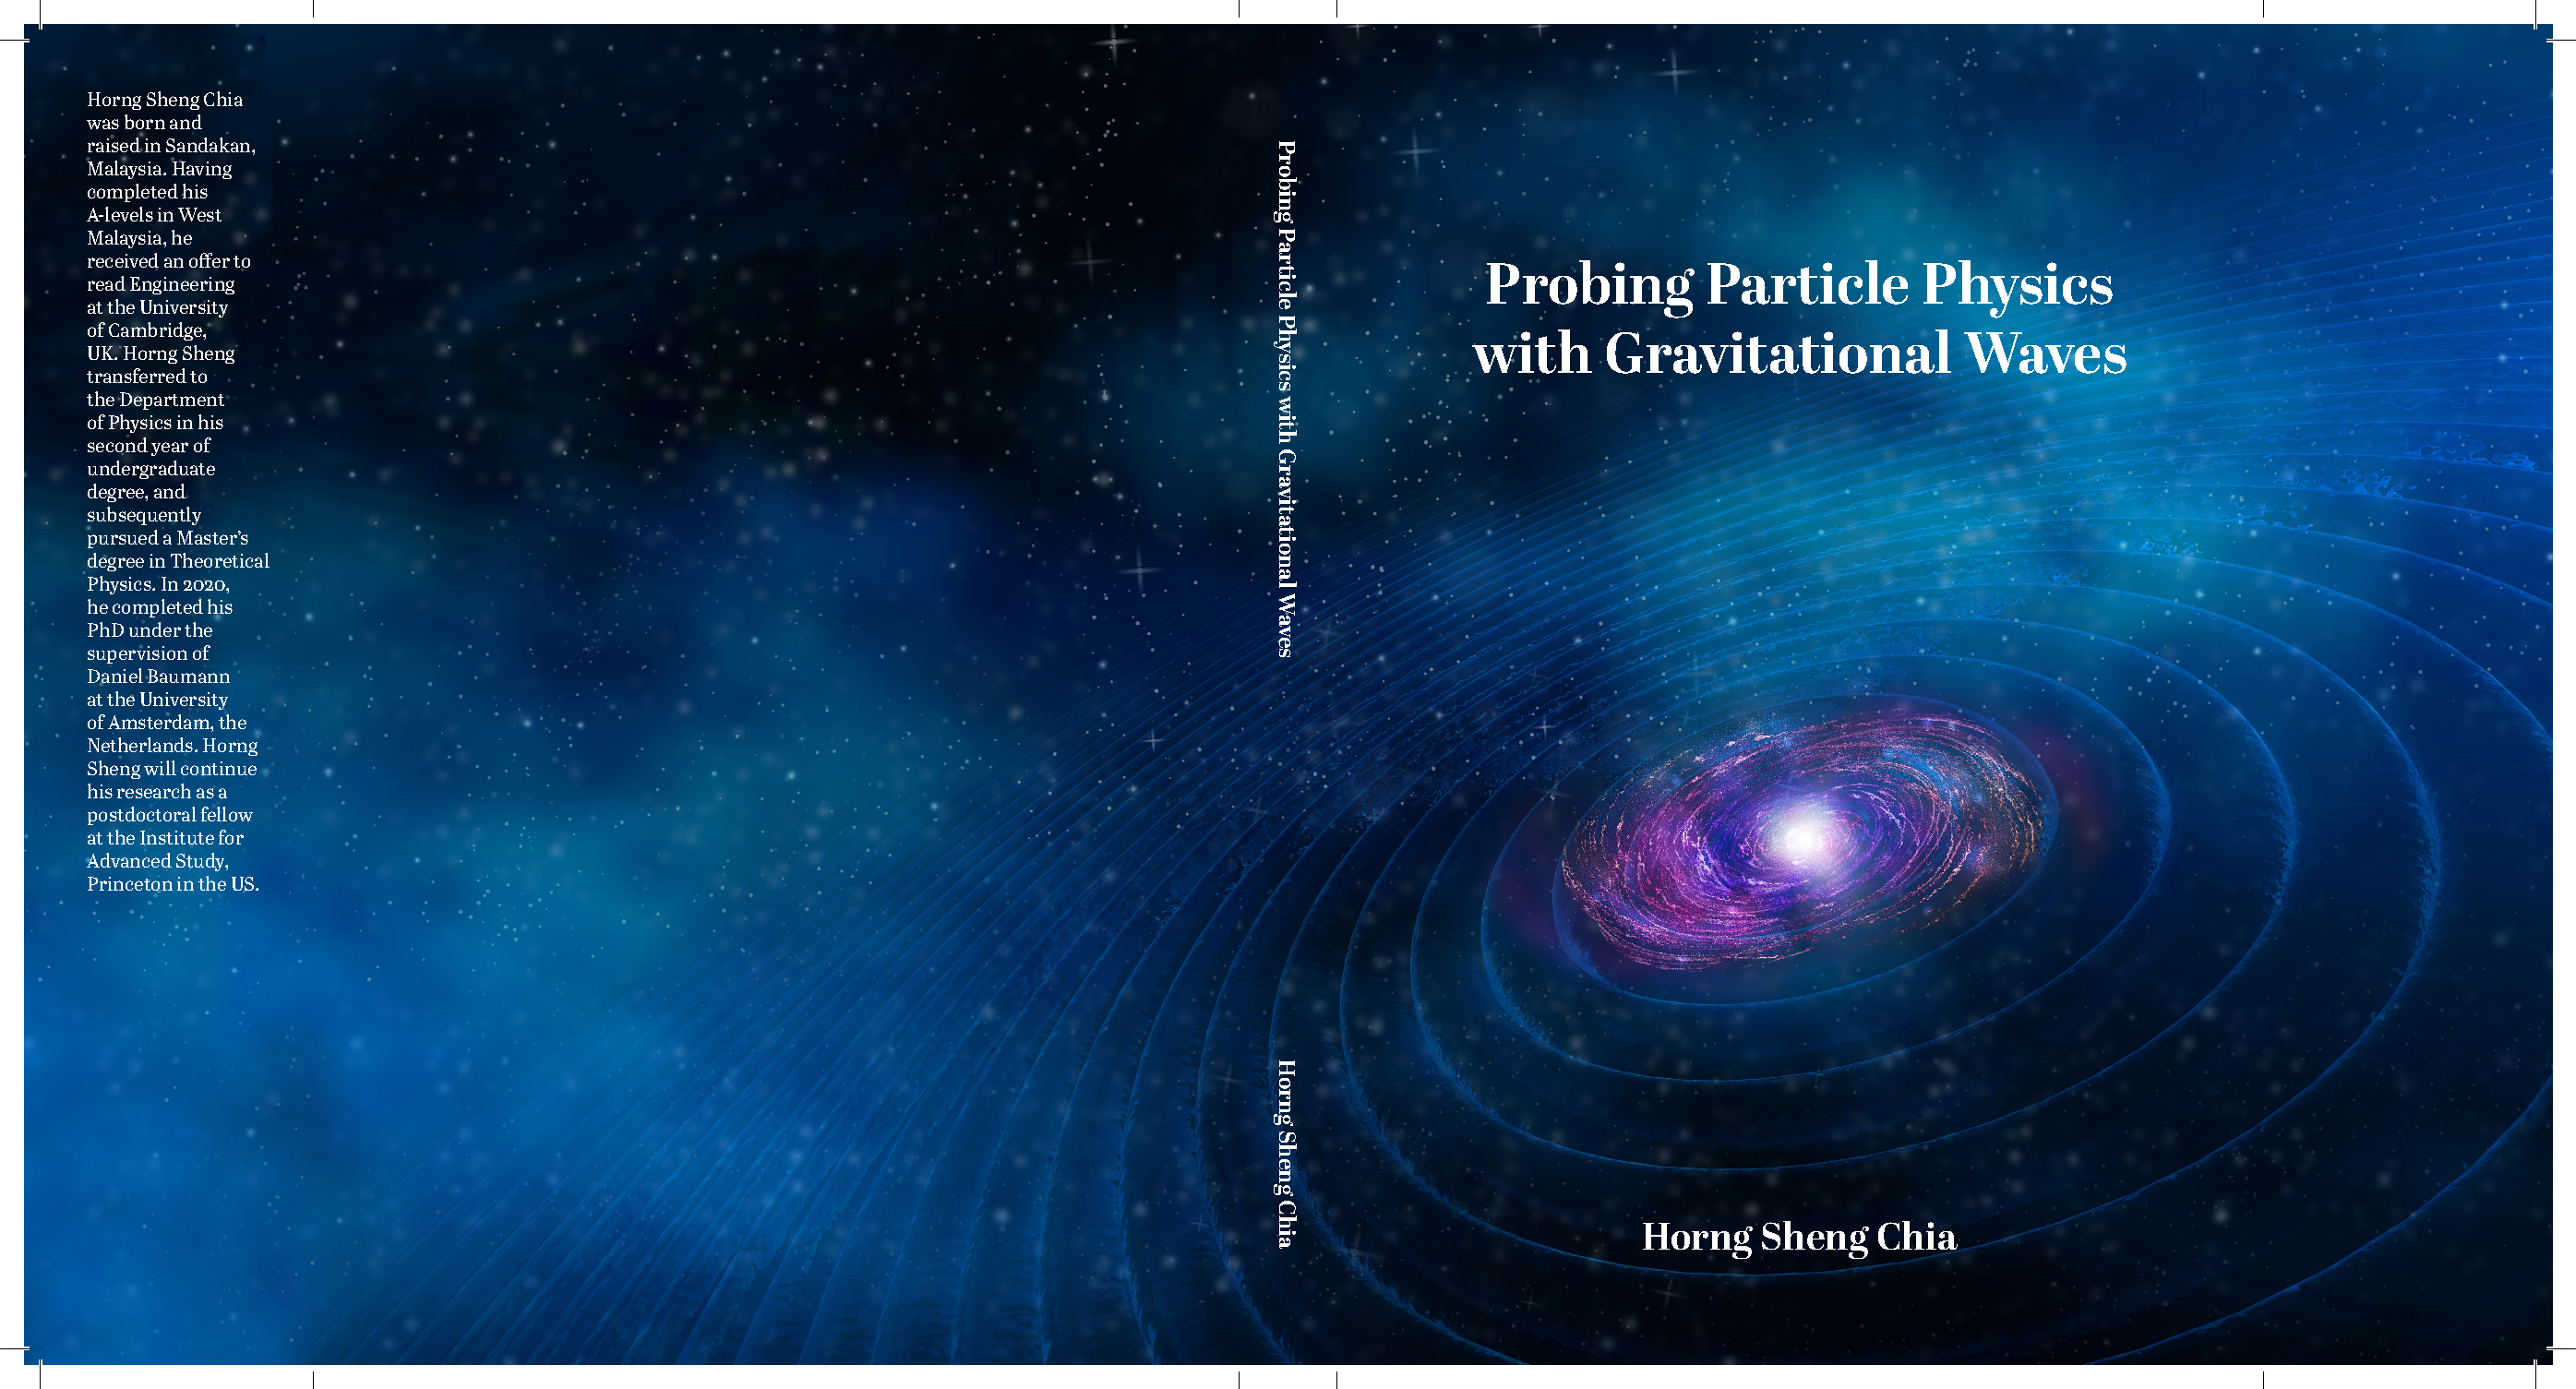
\includepdf[fitpaper]{Cover.pdf}
\let\cleardoublepage\clearpage
\frontmatter
	\maketitle
	}
	
% ======== Publication list ========
\basedon{Publications}{% Publication list ============================================================

{\scshape This thesis is based on the following publications:} \vskip 14pt


\begin{itemize}[]

{\fontfamily{cmr}\selectfont

\item [\cite{Montel:2022fhv}]

{N. Anau Montel}, A. Coogan, C. Correa, K. Karchev, C. Weniger, \textit{Estimating the warm dark matter mass from strong lensing images with truncated marginal neural ratio estimation}, 
\href{https://doi.org/10.1093/mnras/stad2925}{Mon. Not. Roy. Astron. Soc. 527 (2024) 66}, \href{https://arxiv.org/abs/2209.09918}{\ttfamily arXiv:2209.09918}. \vskip 4pt

{All authors participated in the planning of the project. The analysis code was primarily written by NAM with input from AC, KK, and CW. The paper was primarly written by NAM with inputs from all authors.}   \vskip 4pt

Presented in Chapter~\ref{cha:lensing}.\vskip 4pt
 

\item[\cite{AnauMontel:2023stj}] 
{N. Anau Montel}, J. Alvey, C. Weniger, \textit{Scalable inference with Autoregressive Neural Ratio Estimation}, \href{https://doi.org/10.1093/mnras/stae1130}{Mon. Not. Roy. Astron. Soc. 527 (2024) 66},  \href{https://arxiv.org/abs/2308.08597}{\ttfamily arXiv:2308.08597}.  \vskip 4pt

{All authors participated in the planning of the project. The analysis code was primarily written by NAM, except for the stellar stream example contributed by JA. The paper was written by NAM and JA, with input from CW.}   \vskip 4pt

Presented in Chapter~\ref{cha:anre}. \vskip 4pt


\item[\cite{List:2023aa}] 
F. List, {N. Anau Montel}, C. Weniger, \textit{Bayesian Simulation-based Inference for Cosmological Initial Conditions}, Machine Learning and the Physical Sciences Workshop at the 37th Conference on Neural Information Processing Systems (NeurIPS 2023) \href{https://ml4physicalsciences.github.io/2023/files/NeurIPS_ML4PS_2023_218.pdf}{[Paper]} \href{https://nips.cc/media/PosterPDFs/NeurIPS%202023/76248.png}{[Poster]} ,  \href{https://arxiv.org/abs/2310.19910}{\ttfamily arXiv:2310.19910}.  \vskip 4pt

{All authors participated in the planning of the project. FL provided the simulations, NAM and FL wrote the analysis code with input from CW. The paper was written by both NAM and FL, with input from CW.}   \vskip 4pt

Presented in Chapter~\ref{cha:cosmo}. \vskip 4pt


\item[\cite{AnauMontel:2022ppb}] 
{N. Anau Montel}, C. Weniger, \textit{Detection is truncation: studying source populations with truncated marginal neural ratio estimation}, Machine Learning and the Physical Sciences Workshop at the 36th Conference on Neural Information Processing Systems (NeurIPS 2022) \href{https://ml4physicalsciences.github.io/2022/files/NeurIPS_ML4PS_2022_50.pdf}{[Paper]} \href{https://neurips.cc/media/PosterPDFs/NeurIPS%202022/57017.png}{[Poster]} , \href{https://arxiv.org/abs/2211.04291}{\ttfamily arXiv:2211.04291}.  \vskip 4pt

{Both authors participated in the planning of the project. The analysis code was written by NAM with input from CW. The paper was primarly written by NAM with input from CW.}   \vskip 4pt

Presented in Chapter~\ref{cha:detection}. \vskip 4pt

}

\end{itemize}

% Others ============================================================

{\scshape Other publications by the author:} \vskip 14pt

\begin{itemize}[]

{\fontfamily{cmr}\selectfont

 \item[\cite{Coogan:2022cky}] 
A. Coogan, {N. Anau Montel}, K. Karchev,  M. W. Grootes, F. Nattino, C. Weniger, \textit{The effect of the perturber population on subhalo measurements in strong gravitational lenses}, \href{https://doi.org/10.1093/mnras/stac3215}{Mon. Not. Roy. Astron. Soc. 518 (2023) 2746}, \href{https://arxiv.org/abs/2205.09126}{\ttfamily arXiv:2205.09126}.  \vskip 4pt

\item[\cite{Karchev:2022aa}] 
K. Karchev, {N. Anau Montel}, A. Coogan, C. Weniger, \textit{Strong-Lensing Source Reconstruction with Denoising Diffusion Restoration Models}, Machine Learning and the Physical Sciences Workshop at the 36th Conference on Neural Information Processing Systems (NeurIPS 2022) \href{https://ml4physicalsciences.github.io/2022/files/NeurIPS_ML4PS_2022_169.pdf}{[Paper]} \href{https://neurips.cc/media/PosterPDFs/NeurIPS%202022/56913.png}{[Poster]}, \href{https://arxiv.org/abs/2211.04365}{\ttfamily arXiv:2211.04365}. \vskip 4pt

\item[\cite{Correa:2022aa}] 
C. Correa, M. Schaller, S. Ploeckinger, {N. Anau Montel}, C. Weniger, S. Ando, \textit{TangoSIDM: Tantalizing models of Self-Interacting Dark Matter}, \href{https://doi.org/10.1093/mnras/stac2830}{Mon. Not. Roy. Astron. Soc. 517 (2022) 3045}, \href{https://arxiv.org/abs/2206.11298}{\ttfamily arXiv:2206.11298}. \vskip 4pt

%\item[\cite{Correa:2022aa}] 
%{N. Anau Montel}, C. Correa, \textit{TangoSIDM: the effect of dark matter self-interactions on satellite galaxies.},  \vskip 4pt


}

\end{itemize}


\newpage

}

\setcounter{tocdepth}{2}
\tableofcontents

% ======== Body ========
\mainmatter
\chapter{Introduction} \label{sec:introduction}

The fundamental goal of the physical sciences is to understand the laws that govern physical phenomena.
This process inherently involves a continuous interplay between theoretical models and physical observations, forming a feedback loop that continuously refines both. By comparing observational data with model predictions, model validity can be tested, areas of improvements can be identified, and their faithfulness to reality can be improved. Conversely, theoretical models can guide observational strategies by predicting phenomena that have yet to be observed, hence focusing the attention to specific phenomena or conditions that may yield new insights.

%But transforming data into knowledge is still a largely unsolved problem; a problem, that must be tackled by cross-disciplinary efforts.
A key ingredient of this scientific process is \emph{statistics}. Statistics is a rigorous mathematical language that enables formal statements about what events are possible under physical laws, thus bridging the gap between physics models and observational data. Statistics is today at the very heart of the scientific process, and not just an optional nuisance.
Guided by statistical formulation, given some parameters that describe a physical system, implied \emph{predictions} or consequences of a physical model can be computed, allowing for the systematic exploration of the model's implications. Predictions can be either deterministic or intrinsically stochastic, \eg\ due to the randomness of the physical processes, the measurement processes, or incomplete information.
%This approach is known as forward modeling and the above-mentioned physical parameters are called the model parameters.
In order to refine theoretical models, it is essential to perform the inverse process: starting with the effects to discover the causes, inferring from a set of observations the causal factors that produced them. This task, known as solving an \emph{inverse problem} \cite{Groetsch:1993, Aster:2005}, involves mapping back observational data to infer the underlying model parameters that are not directly observable. %, directly answering the question ``which range of physical model parameters is the most probable given my data?". 

In astrophysics, this iterative cycle between prediction and inference is particularly challenging due to the complex nature of the systems under study. In this field, countless statistical methods have been developed over the years, and although rarely in the spotlight, they ultimately determine what is accepted as scientifically established truth. Since an inefficient or incorrect use of statistical data analysis may lead to weaker or entirely wrong conclusions, it is thus of the utmost importance to identify where and how progress is possible in order to advance the field. 


\section{Astrophysical data analysis challenges}\label{sec:astro}

We are at the dawn of a data-driven era in astrophysics and cosmology. As we can see from Figure~\ref{fig:intro-data}, that shows the minimum volume of data per year expected to be produced by a range of recent and upcoming surveys and experiments, the coming decade will see transformative science conducted by observatories, based both on the ground (\eg\ Rubin-LSST \cite{LSSTDarkEnergyScience:2012kar}, ELT \cite{Simon:2019aa}), and space-based missions (\eg\ JWST \citep{Gardner:2006ky}, Euclid \cite{Refregier:2010ss}). Crucially, this wealth of data promises unprecedented high-precision measurements of the growth of structure and geometry of the universe, opening new windows to dark matter \cite{Cirelli:2024ssz, drlicawagner2022reporttopicalgroupcosmic}, dark energy \cite{Mortonson:2013zfa, Huterer:2017buf}, neutrino physics \cite{Boyarsky:2012rt, SajjadAthar:2021prg}, and inflationary cosmology \cite{Baumann:2009ds, Achucarro:2022qrl}.

Given the unprecedented size and detail of these data, connecting theoretical models with this wealth of high-precision observations presents significant challenges, and the scientific return of many upcoming observations is expected to be limited by the efficiency of our statistical inference tools \cite{AlvesBatista:2021eeu, Green:2022hhj}. First, information must be optimally extracted from the data to avoid discarding valuable insights. Second, uncertainties must be correctly treated and thoroughly propagated to ensure accurate scientific statements. Moreover, fully exploiting this data for scientific purposes will require increasingly complex physical models, which bring along higher computational costs, as well as a larger number of uncertain parameters, including those characterizing signal and background systematics. Hence, the need for principled and scalable statistical analyses has never been more critical (for recent reviews on statistical analysis developments in cosmology and astrophysics see Refs.~\cite{Trotta:2017wnx, verde2010statistical, feigelson2021twenty}).

\begin{figure}
    \centering
	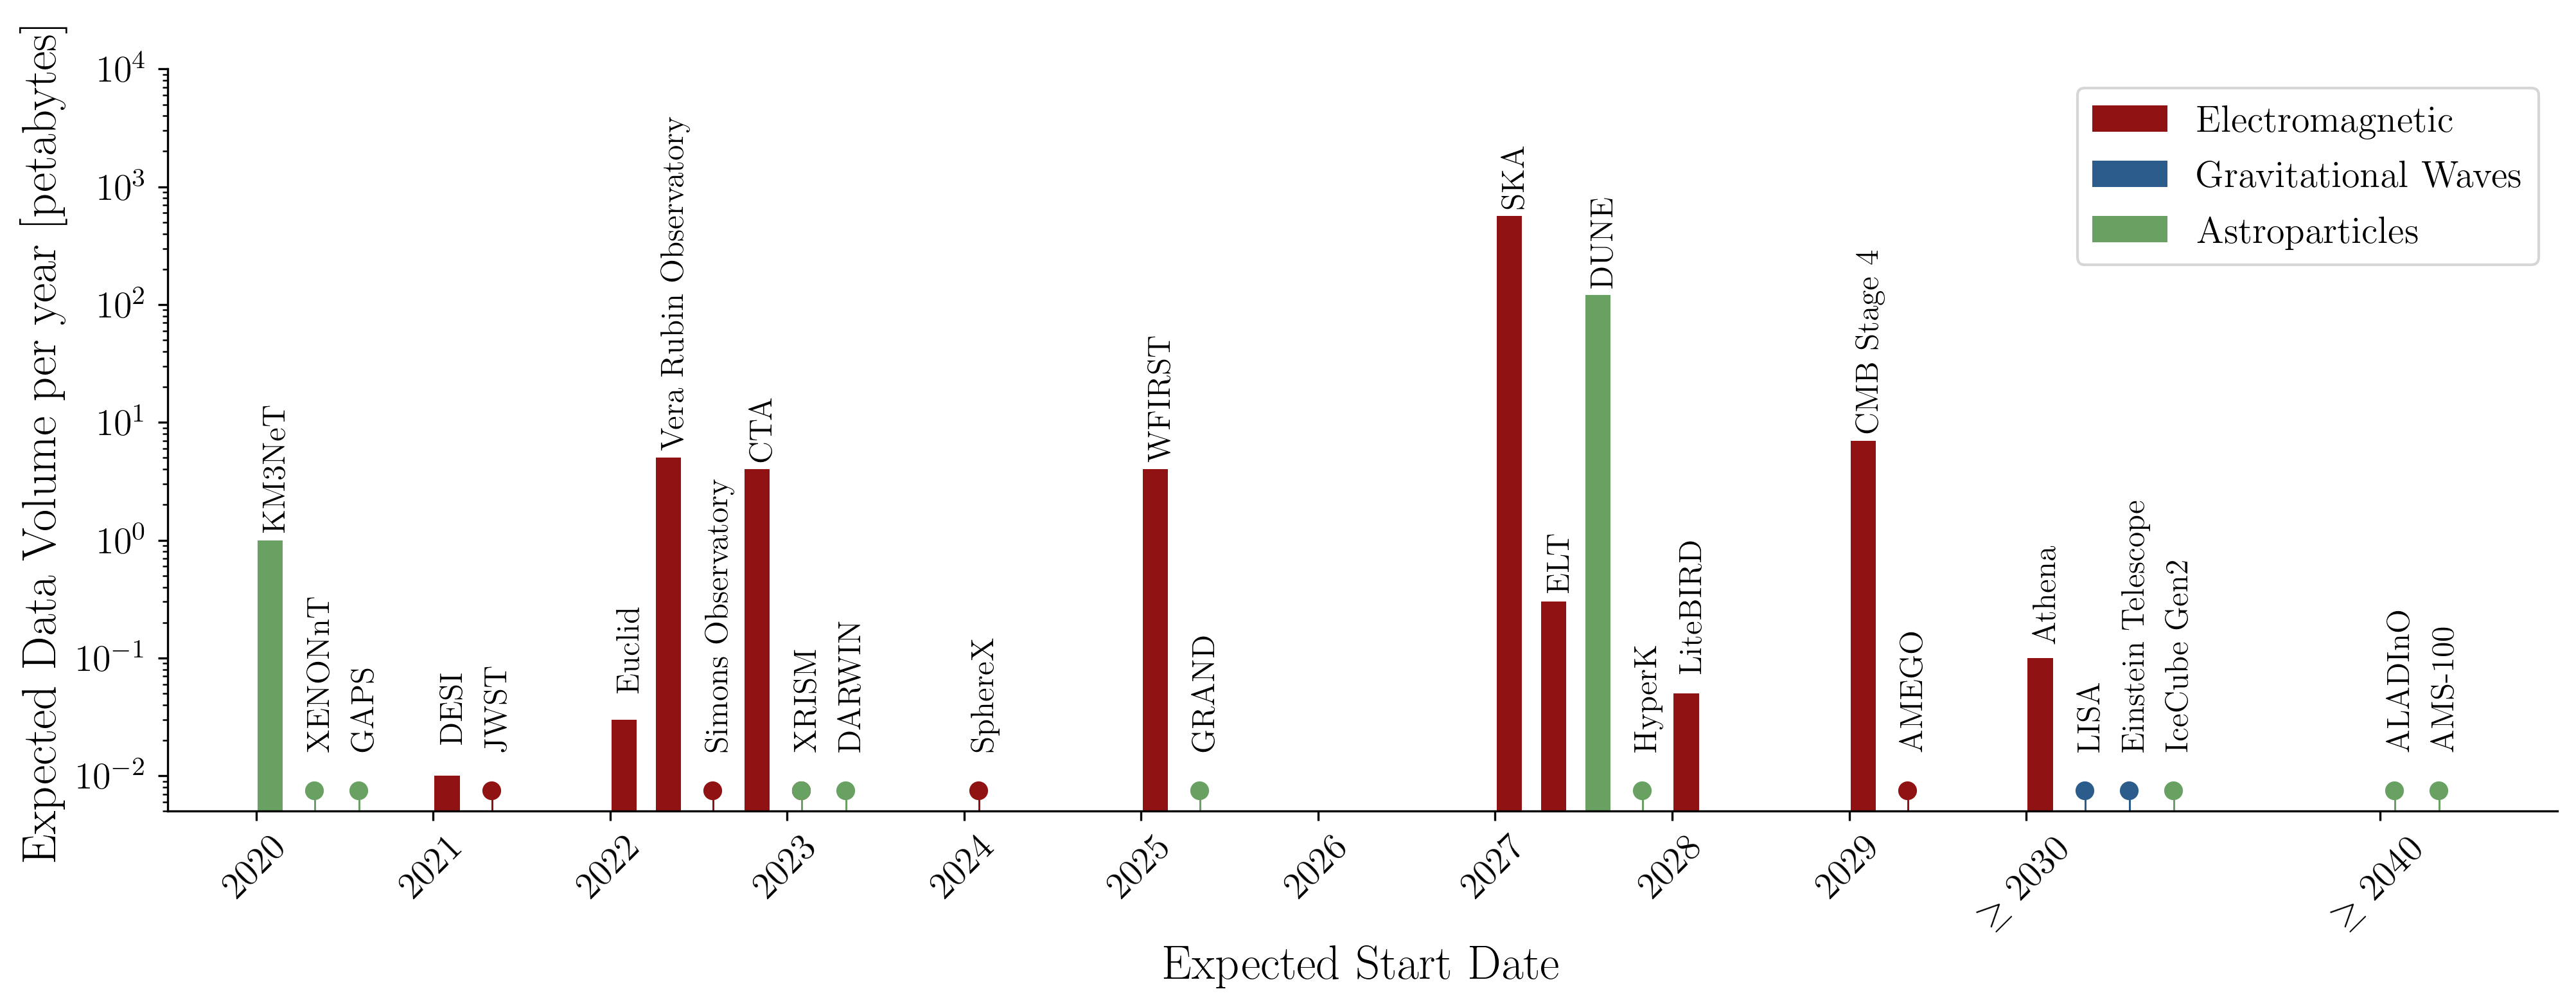
\includegraphics[width=\linewidth]{INTRO-data.png}
    \caption{The graphic shows rough estimates for the minimum expected volume of data per year in petabytes for a range of current and upcoming experiments and surveys in astrophysics and cosmology. Note that both the data volume and start dates are indicative; the plot is intended to give a general overview of the current and future data analysis challenges of the field. The figure and caption are a reproduction of Figure 12 in Ref.~\cite{AlvesBatista:2021eeu}}
    \label{fig:intro-data}
\end{figure}

To get a glimpse of the types of challenges astrophysical data analysis is currently facing, we will now discuss on a high-level some exemplary problems. The selected topics cover only a small part of the current astrophysical statistical analysis challenges, and reflect the works presented in this thesis. %This introductory discussion will serve as their initial motivation, but when relevant, a connection to other statistical problems in physics will be made. 


\paragraph{Strong gravitational lensing}
 - challenges: very large number of degenerate parameters, mixture of parameter inference, object detection, and image reconstruction problem.
        


\paragraph{Cosmology}
    - Field level inference
     non-linear transformations, mixing of spatial structure,
     
     nowledge of the primordial matter density field from which the present non-linear observations formed is of fundamental importance for cosmology, as it contains an immense wealth of information about the physics, evolution, and initial conditions of the universe. Reconstructing this density field from the galaxy survey data is a notoriously difficult task, requiring sophisticated statistical methods, advanced cosmological simulators, and exploration of a multi-million-dimensional parameter space.
     

\paragraph{Point-source in sky maps} 
A striking example of how having higher-resolution data calls for more complex models that needs to account for more objects, hence more parameters, hence harder inference, is given by the evolution of $\gamma$-ray observations in the galactic plane. Starting with SAS-2 satellites (1972-1073), 6 $\gamma$-ray sources and the diffuse emission were identified \cite{Sas26ps, sas2}. Two decades later, with EGRET (1991-2000), it was possible to identify up to 188 $\gamma$-ray sources, extended point sources, and resolve gas emission \cite{Casandjian:2008ky}. With Fermi-LAT \cite{Fermi-LAT:2022byn}, we have now more than 6600  $\gamma$-ray sources, highly resolved gas maps, many extended sources, the detection of the Fermi bubbles \cite{dobler2010fermi}, and an unidentified component, the so called GeV excess \cite{Goodenough:2009gk}. A physical model to describe this type of data can require, \eg, $\mathcal{O}(10^4)$ parameters for the point sources alone. Moreover, some of its components have an unclear uncertainty quantification (\eg\ the gas maps). For this type of data, the statistical analysis can be thought of as a mixture of source detection and image analysis, and requires self-consistent measurement of point-source population parameters based on both on detected and undetected objects.
          
The common thread behind these physical systems and their statistical challenges is that they are formally representable by large models, with the adjective ``large" describing three different properties at the same time: their complexity (in terms of number of components and potentially intricate interactions between them), their volume (in terms of observational data), and the computational resources (in terms of power, memory, and time) needed to solve them. In recent years, new classes of scalable, fast, and computational-efficient inference algorithms have been enabled by breakthroughs in machine learning \cite{Murphy:book}, which could play a major role in the successful analysis of these types of astrophysical data.


\clearpage
\section{The emergence of the simulation-based inference paradigm} \label{sec:paradigm}

Over the years, in order to draw scientific conclusions, an abundance of statistical tools and physics simulation codes have been developed within the community.\footnote{An extensive list of the tools used in astrophysics, cosmology, and high energy physics can be found here: \url{https://github.com/nikosarcevic/HEP-ASTRO-COSMO}.}
In particular, \emph{physics simulators} have always served as powerful predictive devices, mapping model parameters into realized data by reproducing numerically the underlying natural phenomenon of interest.
Recently, remarkable progress in computing technologies and programming languages have made it possible to express increasingly detailed and complex physical models through high-fidelity computer simulators. However, while simulators excel at predicting system behaviors, they are poorly suited for statistical inference and for solving inverse problems. 
Broadly speaking, to evaluate the likelihood of a data realization implicitly defined through a computer simulator one must solve an inverse problem that involves integrating all possible code paths, for all possible simulator configurations, that could have potentially led to the observed data realization. Clearly, as the fidelity and detail of modern computer simulations increase, computing this quantity becomes exceedingly difficult, if not entirely intractable or computationally infeasible  \cite{Cranmer:2019eaq}. 

Fortunately, recent advances in deep learning \cite{lecun2015deep} and differentiable programming \cite{baydin2018automatic} have led to the emergence and proliferation of a \emph{simulation-based inference paradigm} that can effectively tackle the above challenges. By leveraging the power of neural networks, these new methods can approximate the complex relationships within simulators, allowing for efficient solutions to inverse problems that were previously beyond reach \cite{Cranmer:2019eaq}. This paradigm shift in statistical analysis has led to the proliferation of tools for simulation-based inference \cite[\eg][]{Alsing:2019xrx, tejero-cantero2020sbi, Miller2022, lampe} and to their application to various problems in gravitational waves astronomy \cite[\eg][]{Dax:2021tsq, Crisostomi:2023tle, kolmus2024tuning, Dimitriou:2023knw, Vilchez:2024qnw, Bhardwaj:2023xph, Alvey:2023naa, Alvey:2023npw}, strong gravitational lensing analysis \cite[\eg][]{Montel:2022fhv, Wagner-Carena:2020yun, Wagner-Carena:2022mrn, wagnercarena2024strong, Coogan:2022cky, Brehmer:2019jyt, Zhang:2022djp}, cosmological probes \cite[\eg][]{List:2023aa, Tucci:2023bag, Alsing:2019xrx, Modi:2023drt, Makinen:2021nly, DES:2024xij, Jeffrey:2020aa, vonWietersheim-Kramsta:2024cks, Cole:2021gwr, FrancoAbellan:2024tbj, Saxena:2023tue, Karchev:2022xyn, Karchev:2024stw}, and many other astrophysical problems \cite[\eg][]{AnauMontel:2022ppb, Barret:2024kvc, vasist2023neural, Hahn:2022nda, khullar2022digs, Mishra-Sharma:2021oxe, Christy:2024hou, Hermans:2020skz, Alvey:2023pkx, Berteaud:2024zda, Mishra-Sharma:2021nhh}.

We will see more in depth in Chapter~\ref{cha:sbi} the technical details of the various simulation-based inference algorithms, showing how they can improve the quality of insight we can gain from simulations, maximizing information extraction from data, and providing robust uncertainty quantification for scientific statements. In the next introductory section, we will focus on providing the context and motivation for this paradigm shift, comparing it to the likelihood-based paradigm, and highlighting how it can help in tackling some of the challenges discussed previously in Section~\ref{sec:astro}.


\section{To likelihood-base or to simulation-base?}\label{sec:lbi-sbi}

Ultimately, we are interested in inferring the probability distribution of model parameters $\param$ for a given observation $\data_0$. 
%It is therefore important to begin this chapter by clearly clarifying the adopted definition of probability. Throughout this thesis, we will adopt a Bayesian view of probability. In the Bayesian paradigm, probability is a measure of plausibility and simply quantifies an observer belief about how well a quantity of interest can be measured.
In a Bayesian inference context, the posterior distribution for model parameters $\param$ follows from Bayes' theorem
\begin{equation} \label{eq:sbi-Bayes}
    p(\param\mid\data)=\cfrac{p(\data\mid\param)}{p(\data)} \, p(\param) \, ,
\end{equation}
where $p(\data\mid\param)$ is the likelihood of the data $\data$ for given parameters $\param \in \mathbb{R}^D$, $p(\param)$ is the prior probability distribution over the parameters, and $p(\data)$ is the evidence of the data.  
As evident from Equation \eqref{eq:sbi-Bayes}, the Bayesian framework needs both a formalization of the modeling assumptions, encoded by the likelihood, and a prior knowledge associated with each learnable parameter of the model, encoded by the prior. %It acknowledges that learning a model is a subjective task. Occam’s razor says we should always favour the simplest of potential explanations. The Bayesian approach may naturally handle this principle by attributing higher plausibility to simpler model instantiations.
 
Given this Bayesian setup, statistical inference is performed within the context of a probabilistic model $p(\data\mid\param)$, that can be in principle accessed by two different routes. On one hand, \gls*{lbi} algorithms rely on likelihood \underline{evaluations}, single scalars that quantify closeness to the observation $\data_0$. On the other hand, \gls*{sbi} algorithms do not explicitly calculate the likelihood function, but instead rely on \underline{samples} from a stochastic simulator that \emph{implicitly maps} model parameters $\param$ to data $\data$.

\subsubsection{Likelihood-based methods}

The main \gls*{lbi} tools to solve inverse problems for modern astrophysical and cosmological data analysis have been sampling-based inference methods, like \gls*{mcmc} \citep{Metropolis:1953am, Hastings:1970aa} and nested sampling \citep{Skilling:2006gxv, Feroz:2008xx, Ashton:2022grj} techniques. However, it is especially challenging to ensure these methods convergence in high dimensional parameter spaces (the time needed to reach convergence scales poorly with the dimensionality of the explored parameter space), for multi-modal posteriors, and curving degeneracies. More modern methods are taking up these challenges, including Gibbs samplers \cite{Smith:1993gibbs} (that rely on conditional distributions), and slice-sampling techniques \cite{Neal:aa, Handley:2015fda}. For example, the new generation nested sampler \texttt{PolyChord} \cite{Handley:2015fda}, based on slice-sampling, has at worst a $\mathcal{O}(D^3)$ scaling, whereas \texttt{Multinest} \cite{Feroz:2008xx} has an exponential scaling that emerges at high dimensions (see Figure 4 in Ref.~\cite{Handley:2015fda}).

As the dimensionality grows, sampling from the typical set of the posterior distribution becomes exponentially difficult \cite{betancourt2017conceptual}. Therefore, it is useful to resort to gradient-based algorithms, as they are able to concentrate the sampling in high posterior mass regions, despite the large number of model parameters, provided one has efficient access to accurate derivatives of the likelihood function with respect to the model parameters \cite{betancourt2017conceptual}. The most popular gradient-based method among physicist is \gls*{hmc} \cite{Duane:1987hmc, neal2012mcmc}, which is built on the formalism of Hamiltonian dynamics (as the name implies). Widely used in cosmology, it is of particular notice Ref.~\cite{Jasche:2012kq} application to perform dynamical large scale structure inference from galaxy redshift surveys, where the parameter space is the 3D initial matter density field, of order $\mathcal{O}(10^7)$ voxels. This impressive result has been achieved with significant computational resources and by carefully tuning the so called ``mass matrix" of the \gls*{hmc}, which is not always possible. 

Lastly, it is worth mentioning \gls*{vi}, which, differently from the previously mentioned \gls*{lbi} methods, allows for the approximation of extremely high-dimensional Bayesian posteriors with simple proposal distributions by solving an optimization problem \cite{hoffman2013stochastic, zhang2018advances}. As for \gls*{hmc}, \gls*{vi}'s efficient implementation requires gradients from an end-to-end differentiable physical simulator \cite[\eg][]{caustic, Morvan_2021, sstrax}. This can be achieved with little extra effort through auto-differentiation libraries that are standard in deep learning packages \cite[\eg][]{pytorch, jax2018github}. Notably, \gls*{vi} has already been successfully applied in various astrophysical contexts \cite{regier2019cataloging, liu2023variational, Mishra-Sharma:2020kjb, Karchev:2021fro, leike2020resolving}. Of particular notice is Ref.~\cite{regier2019cataloging}, where they jointly optimize parameters for $188\times 10^6$ stars and galaxies using tera-scale datasets. We will come back to \gls*{vi} in Section~\ref{subsec:nsbi}, in order to compare it in details with its direct \gls*{sbi} counterpart. 

\subsubsection{Simulation-based methods}

Differently from \gls*{lbi} methods, \gls*{sbi} entirely relies on samples from a stochastic simulator that maps model parameters $\param$ to data $\data$. This mapping is equivalent to sampling from the model distribution $\data \sim p(\data\mid\param)$, which is effectively an implicit representation of the likelihood. As a result, in this setting one just need a computational code that generates random samples from $p(\data\mid\param)$, that can be later used by a \gls*{sbi} algorithm. For the purpose of this thesis, a \emph{simulator/forward model} is a computer program that takes as input a vector of parameters $\param \in \mathbb{R}^D$, samples a series of internal states or latent variables, and finally produces a data vector  $\data$  as output (usually our observable). Programs that involve random samplings and are interpreted as statistical models are known as probabilistic programs, and simulators are an example \cite{Cranmer:2019eaq}. In principle, using simulators allows for the simultaneous inclusion of all relevant processes that can affect the data, regardless of whether a full probabilistic description is tractable or not, as long as they can be efficiently programmed. In this context, \emph{intractability} means one of two things: a closed-form expression of the likelihood distribution is not available, or even if available it is computationally too expensive, \eg, in the worst case, it scales exponentially with the number of parameters \cite{Leclercq:2018who, Mootoovaloo:2020ott}.

A more detailed exploration of the various \gls*{sbi} algorithms is presented in Chapter~\ref{cha:sbi}, we will now focus on the main high-level differences between \gls*{lbi} and \gls*{sbi}, drawing from the literature to highlight \gls*{sbi} advancements over \gls*{lbi} methods.


\subsubsection{Comparison: SBI vs. LBI}

\begin{figure}
	\centering
	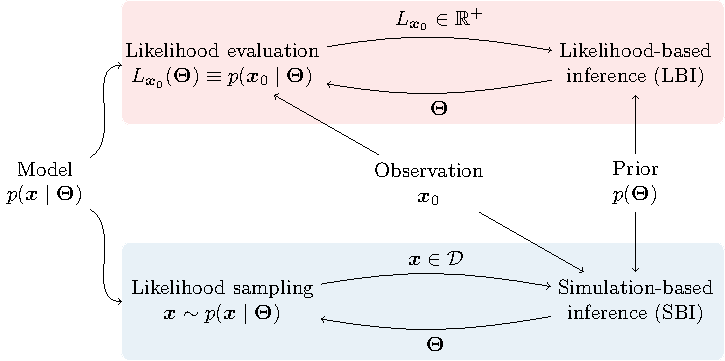
\includegraphics[width=\linewidth]{TikZ/lbi_vs_sbi.pdf}
	\caption{\emph{Likelihood-based} inference algorithms rely on the evaluated likelihood  $L_{\data_0}(\param) $, which is a single scalar that quantifies closeness to the observation $\data_0$. \emph{Simulation-based} inference algorithms learn a function that can be evaluated on many different observations $\data_0$, determining their optimal distance measures case by case. Diagram credits: Christoph Weniger.}
	\label{fig:SBIvsLBI}
\end{figure}

The main differences between \gls*{sbi} and \gls*{lbi} methods are summarized in Figure~\ref{fig:SBIvsLBI}. In both cases, we start with a data model, $p(\data\mid\param$), which describes the probability of data $\data$ given parameters $\param$. In the \gls*{lbi} case, the strategy is a detailed analysis of the likelihood function $L_{\data_0}(\param)$, given an observation $\data_0$. To this end, simplifying, the \gls*{lbi} algorithm will suggest points $\param$ where the likelihood will be evaluated, and try to focus on regions with high density. On the other hand, \gls*{sbi} techniques do \emph{not} require a tractable (see above) likelihood-density $p(\data_0\mid\param)$ at a specific observation $\data_0$. Instead, they rely on synthetic data samples from the likelihood function $\data \sim p(\data\mid\param)$, for a range of model parameters $\param$ that are in the simplest case drawn from the parameter priors, $\param \sim p(\param)$, or in more complex cases from generative models \cite[\eg][]{Karchev:2022aa}. % Essentially, simulation-based techniques are calibrated based on samples from the \emph{generative model} or \emph{joined distribution} $\data, \param \sim p(\data\mid\param)p(\param) \equiv p(\data, \param)$.  

%While \gls*{lbi} produces results with maximal precision and usually the failure mode is over-confidence, the standard failure mode for \gls*{sbi} algorithms is under-confidence (provided correlations between $\data$ and $\param$ are fully identified).

%Classical likelihood-based inference algorithms are problem-agnostic: their performance does not directly depend on the properties, dimensionality or shape of the data $\data \sim p(\data\mid\param)$ for different model parameters $\param$; instead it \textit{only} depends on the shape of the likelihood function as a function of $\param$ for a specific piece of observation $\data_0$, $p(\data_0\mid\param)$.  This is in stark difference to simulation-based, or likelihood-free, algorithms, where the performance of a given algorithm depends critically on how (simulated and real) data $\data$ is processed, interpreted and used.  On first sight, this suggests that simulation-based algorithms are in general more difficult to use, since there are more choices to make.  However, if properly used, simulation-based techniques offer a range of advantages over likelihood-based methods, which we group here into three dimensions, which are also illustrated in 

While in principle the two frameworks converge to the same answer, when applied several practical differences emerge. We will highlight now two of the most striking disparities, but others will surface in the next chapter when the discussion becomes more technical.

\noindent \textbf{Recyclable inference.} As highlighted in Figure~\ref{fig:SBIvsLBI}, the analyzed observation $\data_0$ enters the statistical framework of \gls*{lbi} and \gls*{sbi} at different stages. In particular, \gls*{lbi} algorithms perform inference for a fixed observation $\data_0$, and must rerun from scratch for any another observation. It is thus computationally costly to perform new analysis and statistical test on the obtained results. On the other hand, we will see that \gls*{sbi} algorithms effectively learn an estimate of the probability density function that can be used to perform ``online" inference on any new data (as long as they stem from the same prior support). In this case, there is no need to rerun the whole pipeline for different observations, but just to re-evaluate the learned function on new data.\footnote{This property is not fully preserved in case of sequential \gls*{sbi} algorithms, as they prioritize achieving other types of benefits (this will be illustrated in Chapter~\ref{cha:sbi}).} Furthermore, statistical consistency tests can be performed rather quickly and efficiently. This aspect will be explored in Section~\ref{sec:test}.

\noindent \textbf{Breaking the curse of dimensionality.} When using likelihood-based techniques, in order to solve \emph{one} inference problem, like obtaining samples for marginal posterior of interest, one has to solve \emph{all} of them (joint posterior estimate). The computational overhead of generating joint samples as an intermediate step of marginal inference can be enormous, and can quickly turn an apparently easy inference task, like the measurement of a single physical parameter, into a big challenge. These cases are not uncommon, and, when possible, require problem specific care. For instance, it is common in several scenarios to analytically perform parts of the marginal integrals to reduce the parameter space in clever ways: \eg, in cosmic microwave background analysis by analytically marginalizing over power spectra amplitudes \cite{Gerbino:2019okg}, or in procedure for characterizing the contribution of unresolved point sources by integrating over their positions \cite{Mishra-Sharma:2016gis}, or in strong gravitational lensing analysis by marginalizing over the background source galaxy \cite{Vegetti:2008eg}.
% https://arxiv.org/pdf/1701.06988 point source integration in cross/auto-correlation studies

On the other hand, one key aspect of \gls*{sbi} algorithms in general is their ability to \emph{directly estimate marginal posteriors}, instead of having to first estimate the joint posterior over all parameter space, and then marginalize out nuisance parameters. A clear example of this property can be found in Ref.~\cite{Miller:2020hua}, where both \gls*{sbi} and and a nested sampler are used to sample from an ``eggbox" posterior with $D=14$ dimensions with over $10^4$ modes: the nested sample requires at least $10^7$ samples, whereas \gls*{sbi} needs three order of magnitude less samples to directly estimate the 1-dimensional and 2-dimensional marginal posteriors for the 14 parameters \cite[Figure 2 in][]{Miller:2020hua}. 

A second illustrative example of this property can be found in Ref.~\cite{Cole:2021gwr}. Analyzing cosmic microwave background data, they used \gls*{sbi} to directly estimate marginal posteriors for the six cosmological parameters of interest, while directly marginalizing over the thirteen varying nuisance parameters present in the analysis. The \gls*{sbi} analysis required only $3\times10^3$ simulations, while to obtain the same results using \gls*{mcmc} with the Planck likelihood required $5\times10^6$ simulations (since the \gls*{mcmc} must sample all the nineteen parameters). 

This, and many other comparative analysis of \gls*{sbi} and \gls*{lbi} methods, can be found in Figure~\ref{fig:sbi-lbi-lit}. The figure is meant as a very simplified comparison of \gls*{lbi} and \gls*{sbi} algorithms in the space of number of required simulations (or computational time to run the analysis) versus number of model parameters. Each work addresses different physics applications, each with its own set of challenges and variations, employing diverse types of analysis to solve them. Therefore, each reported scatter point is unique and achieve the reported scaling thanks to different properties of the various \gls*{sbi} and \gls*{lbi} algorithms employed in the specific study. The main take-away message from the plot is that, in general, \gls*{sbi} techniques are extremely scalable and simulation efficient with respect to \gls*{lbi} as a function of model parameters. One of the main reason, except for the fast evaluation time of neural networks, is their possibility to directly estimate marginal probabilities. This effectively means that we can use \gls*{sbi} algorithms to break down large problems into smaller ones, while coherently accounting for the uncertainties coming from the rest of the parameter space (as further detailed in Section~\ref{subsec:tmnre-m}). In the next chapter, we will get deeper into the technical details of \gls*{sbi} and illustrate more reasons why these techniques are promising for pushing the boundaries of the curse of dimensionality compared to likelihood-based methods (Figure~\ref{fig:sbi-lbi-cost}).

\begin{figure}
\centering
\begin{tikzpicture}
	\begin{loglogaxis}[
		width=10cm, height=6cm,
        xmin=1, xmax=1e2,
        ymin=1, ymax=1e9,
        axis line style={black},
        xlabel={{Number of parameters}},
        ylabel={{Number of simulations}},
        tick align=inside,
        minor tick style={draw=none},
        legend style={draw=none}
	]
%	\fill [blue!30, opacity=0.3] 
%		(axis cs:1, 9000) --
%		(axis cs:1e8, 9000) --
%		(axis cs:1e8, 1e8) --
%		(axis cs:1, 1e8) --
%		cycle;
%	\node [blue, align=center] at (axis cs:5e5, 5e4) {Simulation-based inference};
%	\fill [red!30,, opacity=0.3]
%		(axis cs:1, 1e8) --
%		(axis cs:81e2, 1e8) --
%		(axis cs:1, 2e2) --
%		cycle;
%	\node [red, align=center, rotate=38] at (axis cs:4e1, 4e5) {Likelihood-based\\inference};
	% Legend entries
	\addlegendimage{mark=-,red,only marks,mark size=0}
	\addlegendentry{\color{red}LBI}
	\addlegendimage{mark=-,blue,only marks,mark size=0}
	\addlegendentry{\color{blue}SBI}
	\addlegendimage{mark=*,black,only marks,mark size=2}
	\addlegendentry{Ref.~\cite{Cole:2021gwr}}
	\addlegendimage{mark=square*,black,only marks,mark size=2}
	\addlegendentry{Ref.~\cite{Cole:2021gwr}}
	\addlegendimage{mark=triangle*,black,only marks,mark size=2}
	\addlegendentry{Ref.~\cite{Alsing:2019xrx}}
	\addlegendimage{mark=diamond*,black,only marks,mark size=2}
	\addlegendentry{Ref.~\cite{Bhardwaj:2023xph}}
	\addlegendimage{mark=pentagon*,black,only marks,mark size=2}
	\addlegendentry{Ref.~\cite{Vilchez:2024qnw}}
	\addlegendimage{mark=asterisk,black,only marks,mark size=2}
	\addlegendentry{Ref.~\cite{Saxena:2023tue}}
	% Cole
	\addplot[
	    only marks,mark=*, mark size=2pt,red,
	] coordinates {(6, 1e5)};
	\addplot[
	    only marks, mark=*, mark size=2pt,blue,
	] coordinates { (6, 5e3)};
	% Cole
	\addplot[
	    only marks,mark=square*, mark size=2pt,red,
	] coordinates {(19, 5e6)};
	\addplot[
	    only marks, mark=square*, mark size=2pt,blue,
	] coordinates { (19, 3e3)};
	% Alsing
	\addplot[
	    only marks,mark=triangle*, mark size=2pt,red,
	] coordinates {(6, 5e4)};
	\addplot[
	    only marks, mark=triangle*, mark size=2pt,blue,
	] coordinates { (6, 1e3)};
	% Peregrine
	\addplot[
	    only marks,mark=diamond*, mark size=2pt,red,
	] coordinates {(15, 44e6)};
	\addplot[
	    only marks, mark=diamond*, mark size=2pt,blue,
	] coordinates { (15, 72e4)};
	% LISA gw
	\addplot[
	    only marks,mark=pentagon*, mark size=2pt,red,
	] coordinates {(11, 6.41e7)};
	\addplot[
	    only marks, mark=pentagon*, mark size=2pt,blue,
	] coordinates {(11, 1e6)};
	% 21 cm
	\addplot[
	    only marks,mark=asterisk, mark size=2pt,red,
	] coordinates {(2, 1e5)};
	\addplot[
	    only marks, mark=asterisk, mark size=2pt,blue,
	] coordinates { (2, 1e4)};
	
%	- https://arxiv.org/pdf/2403.14750 17 param (lambdacdm + nuisance)
%    - swyft 1.5 h
%    - 3 days mcmc
%- https://arxiv.org/pdf/2404.15402 kids sbi
%    - 20 min
%    - 280 min    
    
	\end{loglogaxis}
\end{tikzpicture}
\caption{Simplified comparison of likelihood-based and simulation-based algorithms in the space of number of required simulations versus number of model parameters. Each work addresses different physics applications, each with its own set of challenges and variations, employing diverse types of analysis to solve them. Therefore, each reported scatter point is unique and achieve the reported scaling thanks to different properties of the various \gls*{sbi} and \gls*{lbi} algorithms employed in the specific study.}
\label{fig:sbi-lbi-lit}
\end{figure}

\begin{figure}
    \centering
    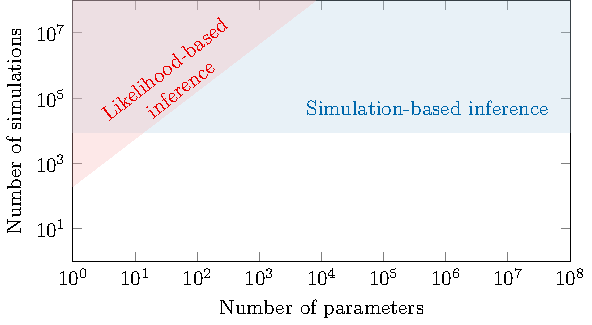
\includegraphics[width=0.8\linewidth]{TikZ/curse_of_dim.pdf}
	\caption{Simplified comparison of likelihood-based and simulation-based algorithms in the space of number of required simulations versus number of model parameters. In general, the simulation requirements of likelihood-based techniques grows significantly with the number of model parameters (curse of dimensionality). Instead, simulation-based inference techniques can, in principle, directly focus on estimating marginal posteriors for parameters of interest, independently of the total number of parameters. This reduces the need for parameter reduction techniques and enables the comparison of complex simulation results with complex data. The figure is adapted from Figure 4 in Ref.~\cite{Boddy:2022knd}.}
    \label{fig:sbi-lbi-cost}
\end{figure}



\section{Outline}

This thesis aims to contribute to the ongoing effort to transition towards simulation-based inference techniques in astrophysics and cosmology, emphasizing some of the tremendous opportunities that this transition brings. To this end, this thesis first proposes a general simulation-based ecosystem for astrophysical data analysis (Chapter~\ref{cha:sbi}). Then, it illustrate its capabilities through exemplary applications to three challenging astrophysical problems, as motivated in Section~\ref{sec:astro}: 
\begin{itemize}[align=left, leftmargin=1cm]
	\item[{\makebox[3.2cm]{Chapters~\ref{cha:lensing} and \ref{cha:anre}: \hfill}}] The analysis of strong gravitational lenses as a dark matter {\makebox[2.45cm]{}} probe.
	\item[{\makebox[3.2cm]{Chapter~\ref{cha:cosmo}: \hfill}}] The reconstruction of cosmological initial conditions from late-{\makebox[2.45cm]{}}time density fields.
	\item[{\makebox[3.2cm]{Chapter~\ref{cha:detection}: \hfill}}] The analysis of point-sources in sky-maps. 
\end{itemize}
Overall, it aims to highlight the potential for fast, flexible, and testable simulation-based algorithms to facilitate scientific discovery in astrophysics and cosmology, at the dawn of their data-driven era, and forward.





\chapter{Simulation-based inference} \label{cha:sbi}
	
The purpose of this chapter is to complement the introduction by laying the foundations of the simulation-based statistical inference framework employed throughout the rest of the thesis. First, we highlight the main differences between simulation-based and likelihood-based approaches, underlining the opportunities that the former brings. We then provide a brief overview of traditional and neural network-based \gls*{sbi} implementations. Lastly, we focus on the specific algorithm that will be employed in the following chapters of this thesis, truncated marginal neural ratio estimation.


\section{To likelihood-base or to simulation-base?}\label{sec:lbi-sbi}

%\section{Bayesian analysis}\label{sec:lbi-bayes}

In scientific analyses, inferring the probability distribution of model parameters $\param$ for a given observation $\data_0$ is a ubiquitous task. It is therefore important to begin this chapter by clearly clarifying the adopted definition of probability. Throughout this thesis, we will adopt a Bayesian view of probability. In the Bayesian paradigm, probability is a measure of plausibility and simply quantifies an observer belief about how well a quantity of interest can be measured.

In a Bayesian learning paradigm, the posterior distribution for model parameters $\param$ follows from Bayes' theorem
\begin{equation} \label{eq:sbi-Bayes}
    p(\param\mid\data)=\cfrac{p(\data\mid\param)}{p(\data)} \, p(\param) \, ,
\end{equation}
where $p(\data\mid\param)$ is the likelihood of the data $\data$ for given parameters $\param$, $p(\param)$ is the prior probability distribution over the parameters, and $p(\data)$ is the evidence of the data.  
As evident from Equation \eqref{eq:sbi-Bayes}, the Bayesian framework needs both an explicit formalization of the modeling assumptions, encoded by the likelihood, and an explicit prior knowledge associated with each learnable parameter of the model, encoded by the prior. %It acknowledges that learning a model is a subjective task. Occam’s razor says we should always favour the simplest of potential explanations. The Bayesian approach may naturally handle this principle by attributing higher plausibility to simpler model instantiations.

\begin{figure}
	\centering
	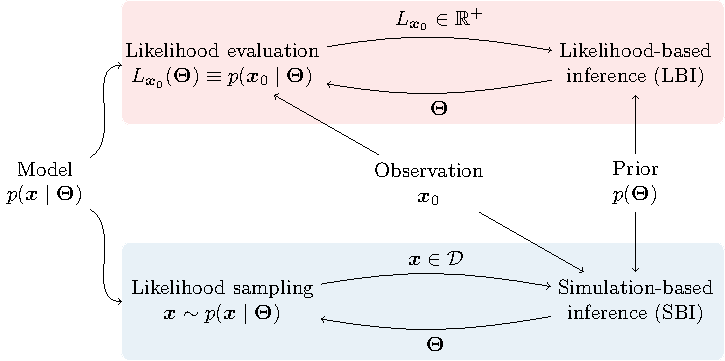
\includegraphics[width=\linewidth]{TikZ/lbi_vs_sbi.pdf}
	\caption{\emph{Likelihood-based} inference algorithms rely on the evaluated likelihood  $L_{\data_0}(\param) $, which is a single scalar that quantifies closeness to the observation $\data_0$. \emph{Simulation-based} inference algorithms learn a function that can be evaluated on many different observations $\data_0$, determining their optimal distance measures case by case. Diagram credits: Christoph Weniger.}
	\label{fig:SBIvsLBI}
\end{figure}

\begin{figure}
    \centering
    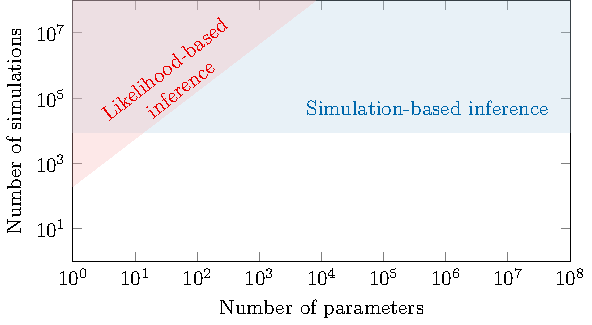
\includegraphics[width=0.9\linewidth]{TikZ/curse_of_dim.pdf}
	\caption{Simplified comparison of likelihood-based and simulation-based algorithms in the space of number of required simulations versus number of model parameters. In general, the simulation requirements of likelihood-based techniques grows significantly with the number of model parameters (curse of dimensionality). Instead, simulation-based inference techniques can, in principle, directly focus on estimating marginal posteriors for parameters of interest, independently of the total number of parameters. This reduces the need for parameter reduction techniques and enables the comparison of complex simulation results with complex data. The figure is adapted from Figure 4 in Ref.~\cite{Boddy:2022knd}.}
    \label{fig:sbi-lbi-cost}
\end{figure}
 
Given this Bayesian setup, statistical inference is performed within the context of a probabilistic model $p(\data\mid\param)$, that can be in principle accessed by two different routes. On one hand, \gls*{lbi} algorithms rely on likelihood \underline{evaluations}, single scalars that quantify closeness to the observation $\data_0$. The main \gls*{lbi} tools to solve inverse problems for modern astrophysical and cosmological data analysis have been sampling-based inference methods like \gls*{mcmc} \citep{Metropolis:1953am, Hastings:1970aa} and nested sampling \citep{Skilling:2006gxv, Feroz:2008xx, Handley:2015fda} techniques. However, these methods often rely on approximate likelihoods, and the time needed to reach convergence scales poorly with the dimensionality of the explored parameter space. More modern methods are taking up this latter challenge, including gradient-based algorithms such as Hamiltonian Monte-Carlo~\citep{Duane:1987de}, or slice-sampling techniques~\citep{Neal:aa, Handley:2015fda}.

On the other hand, \gls*{sbi} algorithms do not explicitly calculate the likelihood function, but instead rely on \underline{samples} from a stochastic simulator that  \emph{implicitly maps} model parameters $\param$ to data $\data$. This mapping is equivalent to sampling from the model distribution $\data \sim p(\data\mid\param)$, which is effectively an implicit representation of the likelihood. As a result, in this setting one just need a computational code that generates random samples from $p(\data\mid\param)$. For the purpose of this thesis, a \emph{simulator/forward model} is a computer program that takes as input a vector of parameters $\param \in \mathbb{R}^D$, samples a series of internal states or latent variables, and finally produces a data vector  $\data$  as output (usually our observable). Programs that involve random samplings and are interpreted as statistical models are known as probabilistic programs, and simulators are an example. In principle, using simulators allows for the simultaneous inclusion of all relevant processes that can affect the data, regardless of whether a full probabilistic description is tractable or not, as long as they can be efficiently programmed. In this context, \emph{intractability} means one of two things: a closed-form expression of the likelihood distribution is not available, or even if available it is computationally too expensive, \eg\ it scales exponentially with the number of parameters.

The main differences between \gls*{sbi} and  \gls*{lbi} methods are summarized in Figure~\ref{fig:SBIvsLBI}. In both cases, we start with a data model, $p(\data\mid\param$), which describes the probability of data $\data$ given parameters $\param$. In the \gls*{lbi} case, the strategy is a detailed analysis of the likelihood function $L_{\data_0}(\param)$, given an observation $\data_0$. To this end, simplifying, the \gls*{lbi} algorithm will suggest points $\param$ where the likelihood will be evaluated, and try to focus on regions with high density. On the other hand, \gls*{sbi} techniques do \emph{not} require a tractable (see above) likelihood-density $p(\data_0\mid\param)$ at a specific observation $\data_0$. Instead, they rely on synthetic data samples from the likelihood function $\data \sim p(\data\mid\param)$, for a range of model parameters $\param$ that are in the simplest case drawn from the parameter priors, $\param \sim p(\param)$. % Essentially, simulation-based techniques are calibrated based on samples from the \emph{generative model} or \emph{joined distribution} $\data, \param \sim p(\data\mid\param)p(\param) \equiv p(\data, \param)$.  

%While \gls*{lbi} produces results with maximal precision and usually the failure mode is over-confidence, the standard failure mode for \gls*{sbi} algorithms is under-confidence (provided correlations between $\data$ and $\param$ are fully identified).

%Classical likelihood-based inference algorithms are problem-agnostic: their performance does not directly depend on the properties, dimensionality or shape of the data $\data \sim p(\data\mid\param)$ for different model parameters $\param$; instead it \textit{only} depends on the shape of the likelihood function as a function of $\param$ for a specific piece of observation $\data_0$, $p(\data_0\mid\param)$.  This is in stark difference to simulation-based, or likelihood-free, algorithms, where the performance of a given algorithm depends critically on how (simulated and real) data $\data$ is processed, interpreted and used.  On first sight, this suggests that simulation-based algorithms are in general more difficult to use, since there are more choices to make.  However, if properly used, simulation-based techniques offer a range of advantages over likelihood-based methods, which we group here into three dimensions, which are also illustrated in 

While in principle the two frameworks converge to the same answer, when applied several practical differences emerge. We will highlight now two of the most striking disparities, but others will surface in the remaining sections of this chapter when the discussion becomes more technical.

\noindent \textbf{Recyclable inference.} As highlighted in Figure~\ref{fig:SBIvsLBI}, the analysed observation $\data_0$ enters the statistical framework of \gls*{lbi} and \gls*{sbi} at different stages. In particular, \gls*{lbi} algorithms perform inference for a fixed observation $\data_0$, and must rerun from scratch for any another observation. It is thus computationally costly to perform new analysis and statistical test on the obtained results. On the other hand, we will see that \gls*{sbi} algorithms effectively learn an estimate of the probability density function that can be used to perform ``online" inference on any new data (as long as they stem from the same prior support). In this case, there is no need to rerun the whole pipeline for different observations, but just to re-evaluate the learned function on new data. Furthermore, statistical consistency tests can be performed rather quickly and efficiently. This aspect will be explored in Section~\ref{subsec:tmnre-test}.

\noindent \textbf{Breaking the curse of dimensionality.} When using likelihood-based techniques, in order to solve \emph{one} inference problem, like obtaining samples for marginal posterior of interest, one has to solve \emph{all} of them (joint posterior estimate). The computational overhead of generating joint samples as an intermediate step of marginal inference can be enormous, and can quickly turn an apparently easy inference task, like the measurement of a single physical parameter, into an enormous challenge. These cases are not uncommon, and require problem specific care, like analytically performing parts of the marginal integrals.

On the other hand, one key aspect of \gls*{sbi} algorithms in general is their ability to \emph{directly estimate marginal posteriors} for parameters of interest, instead of having to first estimate the joint posterior over all parameter space, and then marginalise out nuisance parameters. The possibility to directly estimate marginal probabilities effectively means that we can use \gls*{sbi} algorithms to break down large problems into smaller ones, while coherently accounting for the uncertainties coming from the rest of the parameter space (as further detailed in Section~\ref{subsec:tmnre-m}). This specificity makes SBI techniques extremely scalable and simulation efficient with respect to likelihood-based ones as a function of model parameters, as exemplified in Figure~\ref{fig:sbi-lbi-cost}. 

\section{Background: the landscape of simulation-based inference} \label{sec:sbi}

In this section, we describe the developments and landscape of \gls*{sbi} algorithms. We begin by providing a brief overview of traditional implicit-likelihood methods for posterior inference, approximate bayesian computation and kernel density estimation (Section \ref{subsec:abc}). We then explain the different routes one can use to vastly accelerate and scale this process using neural networks. Lastly, we compare the various neural \gls*{sbi} algorithms by discussing their drawbacks and advantages (Section \ref{subsec:nsbi}). 

%Turning more towards the history and development of \gls*{sbi}, there are two common traditional approaches that use simulations to do statistical inference when the analytic form of the likelihood is intractable. 

\subsection{Traditional \gls*{sbi}}  \label{subsec:abc}

The first implicit-likelihood ideas date back to the 1980s. Particularly relevant for the initial development of this paradigm was statistician Donald Rubin's discussion about the use of frequency calculations for the interpretation of Bayesian statements \cite{rubin1984bayesianly}. Importantly, in these lectures he encouraged statisticians to not settle for analytically tractable models only, but to instead consider computational methods to estimate the posterior distribution of interest for a wider range of models. An outline of the most well-known traditional \gls*{sbi} algorithm, \emph{\gls*{abc}}, can be already found in Rubin's work \cite[Section 3.1]{rubin1984bayesianly}. 

It is worth exploring in more details the \gls*{abc} algorithm, since it will serve us as the classical analogue of the \gls*{sbi} technique mostly employed throughout this thesis (see Section~\ref{sec:tmnre}). For more detailed reviews see Refs.~\cite{marin2012approximate, Sisson:2018aa, Grazian:2019aa}. \Gls*{abc} is a rejection sampling algorithm where, given a prior $\param\sim p(\param)$ proposed samples $\data \sim p(\data\mid\param)$ from the forward model are compared to the target observed data $\data_0$ with a hand-crafted distance measure based on some low-dimensional summary statistics $s(\data)$, as for example
\begin{equation}
    d(\data, \data_0)  = \mid\mid s(\data) - s(\data_0)\mid\mid\;.
\end{equation}
Samples from the approximate posterior are drawn with rejection sampling using an acceptance tolerance $\epsilon$ such that samples satisfy $d(\data, \data_0) < \epsilon$.
Hence the posterior
\begin{equation}
    p_\text{ABC}(\param\mid\data) = \frac
    {\int_{d(\data_0, \data) < \epsilon} d\data\, p(\param\mid\data)p(\data)}
    {\int_{d(\data_0, \data) < \epsilon} d\data\, p(\data)} \;
\end{equation}
is guaranteed to converge to the true one for sufficient summary statistics and for $\epsilon \to 0$, $p_\text{ABC}(\param\mid\data) \xrightarrow{\epsilon \to 0} p(\param\mid\data)$. Whereas, when $\epsilon$ is non-zero, the approximate posterior is guaranteed to be broader than the true one, leading to conservative inference. 

Interestingly, a physical implementation of \gls*{abc}-rejection scheme for a single parameter and a single observation was already constructed by Francis Galton in the late 1800s \cite[Figure 5]{stigler2010darwin}. The device is known today as the Galton board, and often used to demonstrate the central limit theorem \cite{galton1889natural}. Since Rubin's work, \gls*{abc} has been widely adopted in astrophysics and cosmology, including applications to, \eg, galaxy demographics \cite{cameron2012approximate}, galaxy–halo connection \cite{hahn2017approximate}, cosmology \cite{Akeret:2015uha}, galaxy clustering \cite{Ishida:2015wla}, type Ia supernovae \cite{Weyant:2012xe}, and cosmic rays \cite{bourriche2024beyond}.

A second classical approach to \gls*{sbi} was also proposed in the 1980s by Diggle and Gratton \cite{diggle1984monte}. The approach was dubbed ``approximate frequentist computation" by the authors of Ref.~\cite{brehmer2018guide} because of its similarities to \gls*{abc}. Specifically, this method is based on creating a approximate model for the likelihood by estimating the distribution of low-dimensional summary statistics from samples drawn from the simulator with histograms or \emph{kernel density estimation}. The advantage over \gls*{abc} is that it is amortized, meaning that after the initial computational cost for the simulation and density estimation phase, evaluating new data points becomes efficient.
This property makes kernel density estimation-based inference particularly well suited for problems with many i.i.d. observations, a key reason for its widespread use in particle physics measurements \cite{Brehmer:2020cvb}. For example, this approach was used for the discovery of the Higgs boson in a frequentist paradigm \cite{brehmer2018guide}. 

Despite their success, there are some explicit disadvantages of these classical \gls*{sbi} methods that are evident from the above brief description. First, they both rely on low-dimensional summary statistics $s(\data)$ to compare simulations to the data, which may not retain all the information available in the data. Second, they suffer from the curse of dimensionality, with a required simulation budget that increases with the dimensionality of the parameter space. In particular, the acceptance rate of \gls*{abc}'s rejection algorithm vanishes exponentially as the dimensionality of the parameter space increases, thus significantly more simulation budget is needed to reach convergence in high dimensions for $\epsilon \to 0$.

These challenges are tackled in modern \gls*{sbi} algorithms thanks to advances in deep learning \cite{lecun2015deep} and automatic differentiation \cite{baydin2018automatic}. In particular, first, the development of neural network's architectures tailored to various data structures has been fundamental for the processing of significantly more complex data  \cite{lecun2015deep}. This allows for the optimization of learned data features w.r.t. some custom loss, instead of relying on hand-crafted summary statistics. Second, neural network-based algorithms are being actively developed to estimate probability density distributions in high dimensions, overcoming the curse of dimensionality \cite[\eg][]{papamakarios2019neural, papamakarios2021normalizing, Papamakarios:2016ctj}. In the next section, we will discuss the main neural network-based \gls*{sbi} algorithms. 


\subsection{Neural \gls*{sbi}} \label{subsec:nsbi}

Moving beyond the classical \gls*{sbi} approaches, in recent years, a number of new \emph{neural network-based \gls*{sbi}} techniques have been proposed. Bayes' theorem (Equation~\eqref{eq:sbi-Bayes}) hints at a few different approaches for the implementation of neural \gls*{sbi} algorithms, as reviewed in Refs.~\cite{Cranmer:2019eaq, Lueckmann:2021aa}. 

%Broadly, the taxonomy of neural \gls*{sbi} algorithms include neural posterior estimation (NPE) which employs density estimation techniques to directly estimate the posterior $p(\param\mid\data)$ \citep{Papamakarios:2016ctj, Greenberg:2019aa}; neural likelihood estimation (NLE) which instead uses density estimation to learn an approximation to the likelihood $p(\data\mid\param)$ \citep{Papamakarios:2018aa}; and neural ratio estimation (NRE) \citep{Hermans:2019ioj,Miller:2020hua} which uses classifiers to approximate the likelihood-to-evidence or posterior-to-prior ratio $\frac{p(\data\mid\param)}{p(\data)}=\frac{p(\param\mid\data)}{p(\param)}$. In this thesis we will focus on the latter and its extensions.

For example, one possible choice is \emph{\gls*{npe}} \citep{Papamakarios:2016ctj, Greenberg:2019aa}, where one introduces a density estimator $q_\Phi(\param\mid\data)$, parametrized through the weights $\Phi$, which is trained to approximate the posterior for parameters $\param$ given data $\data$,
\begin{equation}
    q^\text{NPE}_\Phi(\param \mid \data) \approx p(\param\mid\data)\;.
\end{equation}
A common loss function used in this context is the forward Kullback-Leibler divergence~\cite{Kullback:1951zyt},
\begin{equation} \label{eq:kld}
    D_{KL}(p \mid\mid q) = \sum_{x} p(x) \log\left(\frac{p(x)}{q(x)}\right) \;.
\end{equation}
Application of this loss function requires that the density estimator is normalized to one, $\int \dd\param\ q^\text{NPE}_\Phi(\param \mid \data)=1$, , which can be guaranteed by using specific network architectures like normalizing flows~\cite{papamakarios2021normalizing}.

Another choice is to perform \emph{\gls*{nle}} \citep{Papamakarios:2018aa}, where one trains an estimator for the likelihood probability density of the data $\data$ given some model parameters $\param$, 
\begin{equation}
    q^\text{NLE}_\Phi(\data \mid \param) \approx p(\data\mid\param)\;.
\end{equation}
Again, specialized network architectures are typically employed to guarantee that $q_\Phi(\data \mid \param)$ is a properly normalized density function.

In this broad taxonomy, Bayes' theorem hints at a last quantity that can be estimated, the likelihood-to-evidence or posterior-to-prior ratio 
\begin{equation}
	r(\param;\data)\approx\frac{p(\data\mid\param)}{p(\data)}=\frac{p(\param\mid\data)}{p(\param)}\; .
\end{equation}
This quantity is approximated using binary classification in \emph{\gls*{nre}}.
In this case, the ratio does not need to be normalized, hence one is free to use any neural network architecture. %, since there is no need to enforce normalization. 
In this thesis we will focus on this last algorithm and its extensions.

\paragraph*{Active learning} The taxonomy of \gls*{sbi} algorithms can be refined further based on whether they use some form of {active learning} to guide the simulator towards parts of the parameter space that are most relevant for a specific target observation $\data_0$. In particular, \emph{sequential} \gls*{sbi} approaches adaptively choose informative simulations by using sequentially refined proposal distributions for the model parameters. They have been reported to outperform and be more simulation-efficient with respect to non-sequential ones across a number of different benchmark tasks \citep{Lueckmann:2021aa} and, \eg, in cosmology \cite{Cole:2021gwr}, in gravitational waves astrophysics \cite{Bhardwaj:2023xph}, and in strong lensing analysis \cite{wagnercarena2024strong}. 

The core intuition behind sequential \gls*{sbi} algorithms is the following: given a single observation of interest, $\data_0$, sampling parameters from the entire prior space to generate training data may not be efficient, since it leads to training data $(\data, \param)$ that has significant variance compared to the target observation $\data_0$. Therefore, for a fixed simulation budget, the training samples contain only limited information about the posterior $p(\param\mid\data_0)$. The alternative proposed by sequential algorithms, in order to increase simulation efficiency, is to draw parameters from an adaptive proposal distribution $p^{(R)}(\param)$, resulting in training data that matches the observation of interest more closely in each sequential round $R$. More details regarding various possible implementations of sequential inference are given in Section~\ref{subsec:tmnre-t}.


\section{Truncated Marginal Neural Ratio Estimation} \label{sec:tmnre}

We will now focus our attention on the main \gls*{sbi} technique employed in this thesis, \gls*{tmnre}. We provide a pedagogical introduction, and show that it forms the core of a fast, accurate and precise approach to solve general parameter inference problems in high-dimensional settings. The approach builds on three key simple ingredients. First, neural ratio estimation (NRE). Second, focus on marginal inference (M).  Third, active learning through prior truncation (T).  We provide a technical description of them in the following sections, emphasizing how they compose well together.

\subsection{Neural Ratio Estimation: ``classification is all you need"} \label{subsec:tmnre-nre}

 Ratio estimation rephrases Bayesian posterior inference as a binary classification problem.
Given an implicitly defined model $\data, \param \sim p(\data, \param) = p(\data\mid\param)p(\param)$, the idea behind ratio estimation is to use a binary classifier to distinguish between data \data\ and parameter \param\ pairs  drawn from two classes labeled by the binary variable $C$:
\begin{align}
    p(\data, \param  \mid C = 1) &= p(\data, \param ) \\
    p(\data, \param  \mid C = 0) &= p(\data) p(\param ) \, .
\end{align}
Concretely, these two distributions correspond respectively to drawing data and parameters jointly from the simulator, $\data, \param \sim p(\data, \param)$, or to drawing data and parameters marginally, $\data, \param \sim p(\data) p(\param)$, by sampling an unrelated set of parameters from the prior versus data from the simulator (this can be simply obtained by scrambling the joint pairs).\footnote{Throughout this thesis we will refer to joint samples as \emph{positive} training examples, and to marginal samples as \emph{negative} training examples.} 

Sampling $C=0$ and $C=1$ with equal probability, the decision function for the Bayes-optimal classifier  \cite{Devroye:1996aa} (\ie~the one that minimizes the Bayesian risk of missclassification) is:
\begin{equation} \label{eq:sbi-classifier}
    p(C = 1 \mid \data, \param) = \frac{p(\data, \param)}{p(\data, \param) + p(\data) p(\param)} \equiv \sigma[ \log r(\param; \data)] \, ,
\end{equation}
where we introduced the sigmoid function $\sigma(y) \equiv 1 / (1 + e^{-y})$. Importantly, the equivalence in Equation~\eqref{eq:sbi-classifier} shows how the Bayes-optimal classifier is related to the  posterior-to-prior, likelihood-to-evidence, or joint-to-marginal distribution ratio:
\begin{equation} \label{eq:sbi-ratio}
    r(\param;\data) \equiv \frac{p(\param \mid \data)}{p(\param)} = \frac{p(\data \mid \param)}{p(\data)} =  \frac{p(\data, \param)}{p(\data) p(\param)} \, .
\end{equation}

Thus, one can gain access to the posterior-to-prior ratio by training a classifier of joint versus marginal pairs, which are easily obtainable with a forward simulator, and subsequently use it for inference. In practice, as the first equality in Equation~\eqref{eq:sbi-ratio} suggests, if the prior is tractable, $r(\param;\data)$ gives direct access to the posterior density:  $p(\param \mid \data)=r(\param;\data)p(\param)$.  Alternatively, one can use $r(\param;\data)$ to weight prior samples, enabling posterior sampling even when the prior cannot be expressed in closed-form.

Often, both the data and the parameters are typically high-dimensional objects, and therefore neural network-based classifiers that are able to process this complex data and be efficiently optimised are a necessary choice.
As proposed by Ref.~\cite{Hermans:2019ioj}, in \gls*{nre} the classifier in Equation~\eqref{eq:sbi-classifier} is a \gls*{nn},  $d_{\bm{\Phi}}(\data, \param)$, that takes as input a parameters-data pair and produces an estimate of the ratio $\hat{r}(\param;\data)$.\footnote{Throughout this chapter we will use the notation $\hat{\square}$ to indicate quantities estimated via \gls*{nn}.} 
The network parameters ${\bm{\Phi}}$ are optimized via stochastic gradient descent to minimize the \gls*{bce}:
\begin{equation}\label{eq:sbi-bce}
\begin{split}
    \mathcal{L}[d_{\bm{\Phi}}(\data, \param)] = &-\int \dd \data  \dd\param \left\{ p(\data, \param) \log d_{\bm{\Phi}}(\data, \param) ] \right. \\
    & \left. + p(\data) p(\param) \log\left[ 1 - d_{\bm{\Phi}}(\data, \param) \right] \right\}\; .
\end{split}
\end{equation}
Therefore, by training a neural network $d_{\bm{\Phi}}(\data, \param)$ to estimate $\hat{r}(\param; \data)$ via this supervised classification task, we obtain an estimate of the posterior through $\hat{p}(\param \mid \data) = \hat{r}(\param; \data) p(\param)$. 

%Critically, training only requires the ability to generate \emph{samples} from the simulator. This makes it straightforward to apply ratio estimation in scenarios where the explicit form of the likelihood cannot be written in closed-form. 


\subsection{Marginalization: focus on the essentials} \label{subsec:tmnre-m} % zero-in on what matters, 

Joined posteriors are commonly a key component of a scientific workflow when analysing real-world data, since access to joint posterior samples exhaustively solves a given Bayesian parameter inference. However, when the number of parameters becomes large (hundreds, thousands, millions), the computational overhead of generating joint samples can be enormous. Furthermore, the full joint posterior $p(\param \mid \data)$ is usually only an intermediate step, and not the goal by itself: in many cases, scientific insight is based on a low-dimensional marginalization of the overly informative joint posterior over nuisance parameters.

Let us consider a model with a full joint distribution
\begin{equation}
	p(\data,\interest, \nuisance) = p(\data\mid\interest, \nuisance)p(\interest, \nuisance) \;,
\end{equation} 
where we have split the set of all model parameters $\param = \{\interest,\nuisance\} \in \mathbb{R}^D$ into parameters of interest $\interest \in \mathbb{R}^d$ (which we want to infer) and nuisance parameters $\nuisance \in \mathbb{R}^{D-d}$ (which we want to marginalise over). 
Formally, the marginal posterior is obtained by integrating the joint posterior over all nuisance parameters
\begin{equation}
	p(\interest \mid \data) = \int \dd\nuisance\ p(\interest, \nuisance \mid \data) \;.
\end{equation}


\begin{figure}
    \centering
	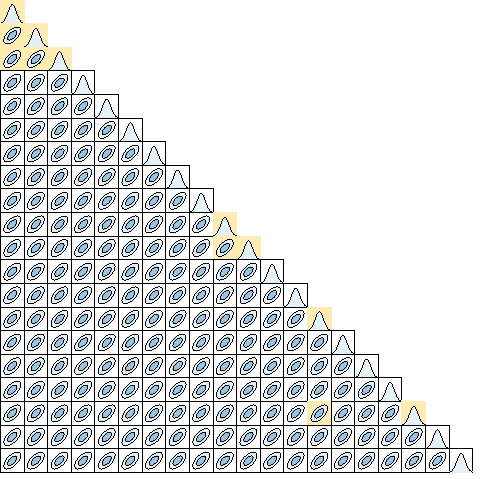
\includegraphics[width=\linewidth]{TikZ/corner.pdf}
    \caption{In simulation-based setting it is possible to directly estimate the marginal posterior of interest, instead of solving the problem for the full joint posterior at once, which can be computationally infeasible for complex models. Here we highlight some of the possible types of marginals that can be directly inferred in \gls*{sbi} for this mock high-dimensional parameter space.}
    \label{fig:sbi-marginals}
\end{figure}


Given the general \gls*{nre} setup, the extension to estimating marginal posteriors is straightforward: parameters to be marginalized over must be \emph{sampled}, but \emph{not presented} to the ratio estimator  \cite{Miller:2020hua}. Hence, marginalization over nuisance variables is done implicitly, since the data will incorporate the variance from the nuisance parameters, but the inference procedure estimates only the marginal likelihood-to-evidence ratio.

In more detail, if $\nuisance$ is not passed to the ratio estimator, the loss function becomes
\begin{align} 
   \mathcal{L}[d_{\bm{\Phi}}(\data, \interest)]&= -\int \dd\data \dd\interest \dd\nuisance\left\{ p(\data,\interest, \nuisance) \log d_{\bm{\Phi}}(\data, \interest,\nuisance) \right. \notag \\
    &\hspace{1.8cm} \left. + p(\data) p(\interest, \nuisance) \log\left[ 1 - d_{\bm{\Phi}}(\data, \interest,\nuisance) \right] \right\} \\
    &= -\int \dd{\data} \dd{\interest} \left\{ p(\data, \interest) \log d_{\bm{\Phi}}(\data, \interest) \right. \notag \\
    &\hspace{1.8cm} \left. + p(\data) p(\interest) \log\left[ 1 - d_{\bm{\Phi}}(\data, \interest) \right] \right\} \;, \label{eq:sbi-bce-m}
\end{align}
where we have integrated over $\nuisance$ to obtain the second equality, proving our statement. 
As a result, the binary classifier trained on $(\data, \interest)$ pairs effectively learns an estimate of the marginal likelihood-to-evidence ratios 
\begin{equation}\label{eq:sbi-ratio_marginal}
    \hat{r}(\data;\interest) \equiv \frac{p(\interest \mid \data)}{p(\interest)} =  \int \mathrm{d}\nuisance \, \frac{p(\boldsymbol{\theta, \eta} \mid \data)}{p(\interest)} p(\nuisance)  \, .
\end{equation}
We can then use the marginal ratio $\hat{r}(\data,\interest)$ to evaluate the marginal posterior for the parameters of interest directly or obtain samples otherwise, with significantly less computational cost. The possibility to directly access marginal posteriors can be easily obtained for  NLE and NPE density estimators as well \cite{Alsing:2019xrx, Jeffrey:2020itg}.

As touched upon in Section~\ref{sec:lbi-sbi}, this way of approaching the problem determines the scalability of \gls*{sbi} algorithms with parameter space dimensionality.
One can then focus on improving the model realism (\ie~complexifying the simulator) without fundamentally altering the inference process (\ie~same ratio estimator training), since there is no need to estimate a full-joint posterior. Effectively this means that we can use \gls*{sbi} algorithms to break down large problems into smaller ones, while coherently accounting for the uncertainties coming from the rest of the parameter space. An exemplification of this process is illustrated in Figure~\ref{fig:sbi-marginals}, where instead of solving the inference problem for the whole parameter space, one can focus on lower-dimensional projections of the correlations. 

It is important to note that, when making the simulator more complex by adding parameters, if all of them contribute equally to the data variance, the implicit data distribution will become noise-dominated. Thus, when referring to scaling to arbitrary number of variables, the data variance is implicitly kept fixed. This limit remains a challenge for likelihood-based methods, but is tractable in the simulation-based frameworks.


\subsection{Truncation: zoom-in for high precision} \label{subsec:tmnre-t}

 The ratio estimators discussed so far are fully \emph{amortized}: that is, they attempt to learn $r(\interest; \data)$ over the whole range of the prior $p(\interest)$. In principle, it is useful to be able to analyze any possible observation with the same network. In practice, when the posterior $p(\interest \mid \data_0)$ for a particular observation $\data_0$ is much narrower than the prior, training an accurate ratio estimator, and general density estimators, requires a massive amount of training data. Hence, for a given limited simulation budget and network bandwidth, amortized inference typically comes at the expense of reduced posterior precision. In order to fully exploit available information in the data with limited computational resources, we instead focus on the problem of \emph{targeted learning} of the posterior for a specific observation of interest $\data_0$ through \emph{sequential inference}. In a nutshell, sequential inference approaches adaptively choose informative simulations by using sequentially refined proposal distributions for the model parameters, as briefly mentioned in Section~\ref{sec:sbi}. In this way, the relevant parameter space is sampled more densely and the network can learn better in that region.

The classification of sequential \gls*{sbi} algorithms can be sifted based on how they acquire new, informative simulations. In particular, the sequential techniques adopted in Refs.~\cite{Papamakarios:2016ctj, Lueckmann:2017aa, Greenberg:2019aa, Papamakarios:2018aa, Hermans:2019ioj, Durkan:2020aa} draw new simulations for the next round from the \emph{approximate posteriors} learned in each round. However, this approach suffers from two limitations. First, several frequently used diagnostic tools for \gls*{sbi} depend on performing inference across multiple observations (\eg~expected coverage tests, see Section~\ref{subsec:tmnre-test}). In this setting, to perform these tests, one would have to generate new simulations and network retraining for each observation, which is often prohibitively expensive. Second, marginal posterior estimation is in general affected by the proposal distribution, since one implicitly integrates over it. As a result, this approach is unsuitable for learning multiple marginal posteriors simultaneously over a number of sequential rounds, since sampling from the marginal for a particular parameter may hinder learning the marginals for other parameters (for a possible workaround see Ref.~\cite{Alsing:2019xrx}).

To overcome the limitations of this sequential scheme, Ref.~\cite{Miller:2021aa} proposed a hard-likelihood \emph{prior truncation} scheme, applicable to \gls*{nre}, that composes well with marginalisation and is locally amortised.\footnote{With \emph{locally amortised} inference we refer to an inference that can be repeated several times, without retraining, with distinct observations that live in the support of the truncated prior.}
This prior truncation scheme iteratively discards in rounds $R$ low likelihood(-to-evidence) regions, where the current approximate likelihood-to-evidence ratio evaluated for the target observation is below a user defined threshold $\epsilon$. Concretely, this means keeping the region of parameter space defined by
\begin{equation}\label{eq:gamma_r}
    \Gamma^{(R)}_{\interest} = \{ \interest \in \mathbb R^d : \hat{r}^{(R)}(\interest ; \data) > \epsilon\} \;,
\end{equation}
and discarding its complement.\footnote{Similar truncated proposals have also been introduced in \cite{Deistler:2022aa} in the context of NPE, where the condition is instead on the current estimated posterior, \eg~$\hat{p}^{(R)}(\interest \mid\data) > \epsilon$.
}
Such truncated priors constrained to the parameter region $\Gamma^{(R)}_{\interest}$ can be defined as:
\begin{equation}
    \label{eqn:truncated_prior}
    p_\Gamma(\interest) \equiv  \frac1V \mathbb{I}_{\Gamma}(\interest) p(\interest)\;.
\end{equation}
Here, $\mathbb{I}_{\Gamma}(\interest)$ is an indicator function, which is one for $\interest \in \Gamma$ and zero otherwise,
\begin{equation}
\mathbb{I}_\Gamma(\interest) \equiv \left\{
\begin{matrix}
1 \quad \text{for} \quad \interest \in \Gamma\\
0 \quad \text{otherwise}
\end{matrix}
\right.
\end{equation}
Furthermore,  $V \equiv \int d\interest\, \mathbb{I}_\Gamma(\interest)\, p(\interest)$ is a normalizing constant that can be interpreted as the mass of the truncated prior.

The prior truncation scheme thus defines a series of nested indicator functions $\mathbb{I}_{\Gamma^{(R)}}$ whose regions have the property $\Gamma^{(0)}  \supset \Gamma^{(1)}  \supset \Gamma^{(2)} \supset \dots \supset \Gamma^{(S)}$, where $\Gamma^{(0)}$ defines the support of the full initial prior, and $\Gamma^{(S)}$ is the final stable truncated prior. We illustrate this truncation procedure for a simple 1-dimensional scenario in Figure~\ref{fig:sbi-truncation}.

\begin{figure}
	\centering
	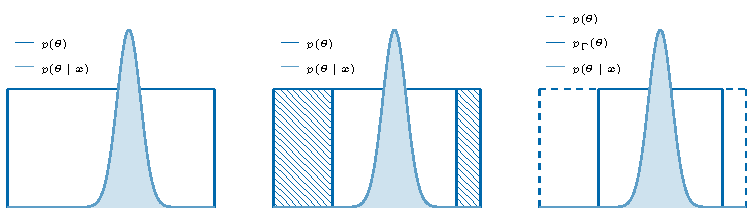
\includegraphics[width=\linewidth]{TikZ/truncation.pdf}
	\caption{Illustration of sequential inference for a 1-dimensional posterior. First, we learn an approximation to the posterior $p(\interest\mid\data)$ from the full initial prior $p(\interest)$. Then, we restrict the prior in the region where the parameter $\interest$ is likely to have generated $\data$. In the next inference round, the truncated prior $p_\Gamma(\interest)$ will be used to generate targeted simulations, sampling the parameter space more densely in the region of interest, so that the network can learn better in that region.}
	\label{fig:sbi-truncation}
\end{figure}

Importantly, since this sequential scheme does not modify the shape of the prior proposal distribution, but only restricts its support, the inference is still locally amortised in the constrained proposal distribution region, thus allowing for the possibility of tests that rely on performing inference across multiple observations (in the $\Gamma$ support). Moreover, it is also possible to use the same training data generated for a round to efficiently train arbitrary marginal posteriors for any set of model parameters. 

Training targeted ratio estimators is achieved by replacing the full prior with a \emph{truncated prior} $p^{(R)}_{\Gamma}(\interest)$, where the parameters are restricted to a region $\Gamma$ where they are likely to have generated $\data_0$. Since parameters from the complement of $\Gamma$ are unlikely to have generated $\data_0$, training a ratio estimator with data generated from the truncated prior as opposed to the full prior has little impact on the posterior learned by our ratio estimators. Indeed, only those regions where $p(\data_0 \mid\interest)$ is sufficiently negligible are removed, such that $p(\data_0\mid\interest) \to \mathbb{I}_\Gamma(\interest) \cdot p(\data_0\mid\interest)$ remains an accurate approximation for a given target observation $\data_0$. For generous enough $\Gamma$, the posterior remains essentially unchanged far into its tails,
\begin{equation}
\begin{split}
    p_\Gamma(\interest\mid\data) 
    &= \frac{p(\data\mid\interest)\,p_\Gamma(\interest)}{\int d\interest\, p(\data\mid\interest)\, p_\Gamma(\interest)}
    = \frac{p(\data\mid\interest)\,p(\interest)\cdot\mathbb{I}_\Gamma(\interest)\, V^{-1}}
    {\int d\interest\, p(\data\mid\interest)\,p(\interest)\cdot \mathbb{I}_\Gamma(\interest)\, V^{-1}} \\
    &\simeq \frac{p(\data\mid\interest)p(\interest)}{p(\interest)}
    = p(\interest\mid\data) \;. 
\end{split}
\end{equation}

%In practice, since the highest probability density region of the true posterior $\Gamma$ is unknown, we compute an estimate $\hat{\Gamma}$ over a sequence of inference rounds. At the beginning of each round, we sample from $p_{\hat{\Gamma}}(\interest)$ (or the full initial prior in the first round) and train a ratio estimator. We re-estimate $\hat{\Gamma}$ by keeping only the parts of the previous truncated prior for which $\hat{r}(\interest; \data)$ exceeds a certain threshold \cite{Miller:2021aa}. This determines the truncated prior for the next round. The final ratio estimator is obtained when $\hat{\Gamma}$ stops changing substantially between rounds, even when using more training data. 

This whole scheme relies on the assumption that posterior estimate $\hat p_{\Gamma}(\interest \mid \data_0)$ is a good approximation of $p(\interest \mid \data_0)$. An over-confident estimate would remove parameter ranges that are part of $\Gamma^{(R)}(\interest)$. In practice, this effect is not observed for a conservative choice of $\epsilon$. Moreover, one can test the convergence of the sequential scheme by checking whether high probability regions of the estimated posteriors intersect with the boundaries of the indicator function.


\subsection{Information maximizing neural network} \label{subsec:tmnre-nn}

From a practical perspective, a given inference involves training several classifiers (corresponding to the various marginal ratio estimators) in parallel. For complex and high-dimensional data, it is generally useful to compress it before it is input into the inference network through a so-called compression/summary/embedding network. Hence, the inference neural network usually employed to perform \gls*{tmnre} are generally split into two distinct components: an embedding network $C_\Phi(\data)$ and binary classification networks $d_\Phi(\data, \interest)$. 

The embedding network learns to compresses the potentially high-dimensional data into a low-dimensional feature vector, estimating the best possible summary statistics from the full input data, $\boldsymbol{s}= C_\Phi(\data)$. In principle, the compression network can be any sufficiently expressive network, no specialized network architectures are required. In practice, for faster convergence and better results specific inductive biases of different network architectures should be exploited, \eg~for image data, convolutional neural networks are often appropriate. Throughout this thesis, we will see various example of this (\eg~see Chapter~\ref{cha:lensing}). Furthermore, the compression network output can be shared as input to all of the classification networks, or subdivided between the classifiers, in order for each compressed summary to be optimized for the specific marginal estimator. 

While the purpose of the embedding network is to efficiently summarize data, the purpose of classifiers $d_\Phi(\boldsymbol{s}, \interest)$ is to learn the correlation between the data summary $\boldsymbol{s}$ and the parameters of interest $\interest$ in order to perform the actual ratio estimation. Their inputs are the learned summaries of the observational data concatenated with the parameters of interest for the targeted marginal. Usually, the classifiers are parameterized with fully connected layers and unless otherwise specified in this thesis we will be using the ResNet \cite{he2016deep} architecture as implemented in \swyft \cite{Miller2022}.

The compression network and ratio inference are \emph{optimized simultaneously}, in contrast to other algorithms in the literature, minimizing the \gls*{bce} loss function (Equation~\eqref{eq:sbi-bce-m}). The structure of a general network architecture can be expressed as:
\begin{equation}\label{eq:nn-c}
    d_\Phi(\boldsymbol{s}= C_\Phi(\data), \interest) \simeq  d_\Phi(\data, \interest)  = \sigma[ \log \hat{r}(\interest; \data)] \;,
\end{equation}
and is illustrated in Figure~\ref{fig:sbi-nn}.

\begin{figure}
    \centering
	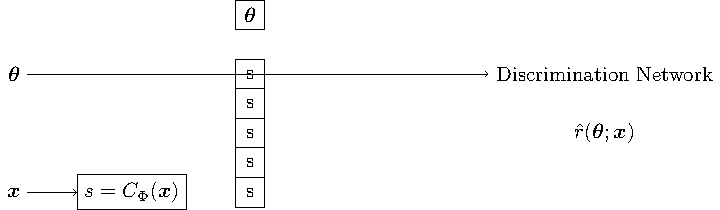
\includegraphics[width=\linewidth]{TikZ/sbi_nn.pdf}
    \caption{\todo{Finish} Illustration of the network architecture, including the embedding network $C_\Phi(\data)$ and the discrimination network $d_\Phi(\boldsymbol{s}, \interest)$. Input data $\data$ and parameters $\interest$ are internally mapped to the marginal parameter combinations of interest, for which individual ratio estimators with a shared compression network are trained. The outputs are estimated ratios for the marginal posteriors of interest... \todo{Finish}}
    \label{fig:sbi-nn}
\end{figure}

\medskip

It is interesting to understand why the approximately equal sign in Equation~\eqref{eq:nn-c} holds and which features $\boldsymbol{s}$ are learned by the embedding network during training, \eg~in comparison to the hand-crafted ones employed in \gls*{abc} (Section~\ref{sec:sbi}). Following Ref.~\cite{Cole:2021gwr}, the \gls*{bce} loss in Equation~\eqref{eq:sbi-bce-m} can be written in terms of the Jensen-Shannon divergence (JSD) as
\begin{equation}
   \mathcal{L}[d_{\bm{\Phi}}(\data, \interest)] = 2 \log2 - 2\mathbb{E}_{p(\data)}\left[D_{JS}(p(\interest\mid\data)\mid\mid p(\interest)\right] \;,
\end{equation}
which follows\footnote{
   In fact,
   \begin{multline}
   -2\mathbb{E}_{p(\data)}\left[D_{JS}\left(p\left(\interest\mid\data\right) \parallel  p(\interest)\right)\right] \\
   =-\mathbb{E}_{p(\data)}\left[
      D_{KL}\left(p\left(\interest\mid\data\right) \parallel \frac12\left(p\left(\interest\mid\data\right) + p(\interest)\right)\right)
      +D_{KL}\left(p\left(\interest\right) \parallel \frac12\left(p\left(\interest\mid\data\right) + p(\interest)\right)\right)\right]\\
   = -\int d\data\, d\interest\,
   \underbrace{p(\data)p(\interest\mid\data)}_{\to p(\data, \interest)} \ln \frac{p\left(\interest\mid\data\right) }{ \frac12\left(p\left(\interest\mid\data\right) + p(\interest)\right)}
   +p(\data)p(\interest) \ln \frac{p\left(\interest\right) }{ \frac12\left(p\left(\interest\mid\data\right) + p(\interest)\right)}\\
   = -\int \dd{\data} \dd{\interest} \left\{ p(\data, \interest) \log d_{\bm{\Phi}}(\data, \interest) \notag + p(\data) p(\interest) \log\left[ 1 - d_{\bm{\Phi}}(\data, \interest) \right] \right\} \\
   = \mathcal{L}[d_{\bm{\Phi}}(\data, \interest)] - 2\ln 2 \;,
\end{multline}
where the third equation follows from Equation~\eqref{eq:sbi-classifier}.
}
directly from the definition of the JSD
\begin{equation}
    D_{JS}(p\mid\mid q) = \frac{1}{2}D_{KL}(p \parallel m)+\frac{1}{2}D_{KL}(q \parallel m)\;,
\end{equation}
where $m=(p+q)/2$ and $D_{KL}$ denotes the Kullback-Leibler divergence, previously defined in Equation~\eqref{eq:kld}.

We can now apply the same logic to our network with a compression step, an information bottleneck, in Equation~\eqref{eq:nn-c}. The posterior is then conditioned on the summary statistics $\boldsymbol{s}$, and the loss function can be written as
\begin{equation} \label{eq:loss-jsd}
   \mathcal{L}[d_{\bm{\Phi}}(\boldsymbol{s} = C_\phi(\data), \interest)] = 2 \log2 - 2\mathbb{E}_{p(\data)}\left[D_{JS}(p(\interest\mid\boldsymbol{s} = C_\phi(\data))\mid\mid p(\interest)\right] \;.
\end{equation}
%thus, data summaries $\boldsymbol{s}$ are learned such that they maximize the JSD between posteriors and priors.  

Looking at Equation~\eqref{eq:loss-jsd}, assuming a fully converged classifier and the loss as a function of the summary $\boldsymbol{s}$, it becomes now evident that a data summary $\boldsymbol{s}$ that minimizes the \gls*{bce} loss has to \emph{maximize} the expected JSD between the data-summary-based posterior and the prior for the parameters of interest $\interest$. Therefore, data summaries $\boldsymbol{s}$ that sufficiently describe data $\data$ for a parameter $\interest$ lead to posteriors $p(\interest\mid\data)$. On the other hand, inefficient data summaries will lead to wider posteriors which are more similar to the prior, reducing the JSD, and increasing the value of the loss function.  Hence, it makes sense to expect that the data summaries that are learned are the most informative to discriminate between samples from the posterior and the prior, or, equivalently, to discriminate whether the likelihood-to-evidence ratio is larger or smaller than one,
\begin{equation}
    \frac{p(\boldsymbol{s} \mid \interest)}{p(\boldsymbol{s})}  = 
    \frac{p(\interest\mid \boldsymbol{s})}{p(\interest)} 
    \lessgtr 1\;.
\end{equation}


%What does a large JS-divergence signify? To see this, we consider the average Bayesian probability of error of wrongly classifying a parameter-data pair as drawn from the prior or the posterior, which is given by
%%
%\begin{equation}
%    \hat P_e = \mathbb{E}_{\data \sim p(\data)} \left[\frac12 \min(p(\interest\mid\data), p(\interest))\right]
%\end{equation}
%%
%In Ref.~\cite{XYZ} it was shown that the minimum of the NRE loss provides an upper bound on the error rate,
%%
%\begin{equation}
%    \hat P_e
%    \leq
%    2\log 2 -  
%    2 \mathbb{E}_{\data\sim p(\data)}\left[D_{JS} ( p(\interest\mid\data) \;\mid\mid\; p(\interest))\right]
%    \leq \ell_{NRE}[F_\phi]\;.
%\end{equation}
%
%When using NRE as described above, the summary is optimized such that it minimizes (an upper bound on) the error rate when classifying points as drawn from the prior vs. drawn from the posterior, or (equivalently) whether the likelihood-to-evidence ratio is larger or smaller than one,
%%
%\begin{equation}
%    \frac{p(\boldsymbol{s} \mid \interest)}{p(\boldsymbol{s})}  = 
%    \frac{p(\interest\mid \boldsymbol{s})}{p(\interest)} 
%    \lessgtr 1\;.
%\end{equation}

%\subsection{Hierarchical inference} \label{subsec:tmnre-hierarchical}
%\todo{Add brief paragraph about hierarchical inference in SBI to setup the problem for populations of subhalos in lensing and point sources in maps?} 
%
%When analyzing real-world data it is common to work with event ensembles, which comprise sets of observations that collectively constrain the parameters of an underlying model of interest. Such models often have a hierarchical structure, where “local” parameters impact individual events and “global” parameters influence the entire dataset. 
%Datasets composed of multiple samples are ubiquitous in scientific and more broadly real-world data analysis tasks. These datasets are typically governed by underlying models that exhibit a rich hierarchical structure, with local parameters shaping individual events while global parameters exert influence across the entire dataset. This layered structure, if appropriately utilized, can greatly augment the efficiency and effectiveness of the inference process.
%We substantiate theoretically as well as empirically the fact that hierarchy-aware inference in many implicit models with a hierarchical structure requires a dataset-wide approach, contrasted with the more common paradigm of combining implicit likelihood or posterior estimators associated with individual observations.
%
%The joint probability distribution of a set of events with cardinality N, with global parameters of interest θ, global nuisance parameters θν as well as local parameters zi can be written as:
%N
%p({x} | {z},θ,θν) = Yp(xi | zi,θ,θν), (1)
%i=1
%
%come from different stellar populations have different intrinsic prop
%Hierarchical Bayesian modelling, however, comes at the cost of having to infer individual parameters for each observed SN Ia, and so the computational burden scales with the data set size
% population variability 
%perform simulation-based inference over event ensembles and can deal with datasets of varying cardinality\cite{Heinrich:2023bmt}

\subsection{Testing SBI: getting it right} \label{subsec:tmnre-test}

\gls*{tmnre} is a \emph{locally amortized} technique, meaning that the ratio estimator are trained to learn a function, that can then be evaluated to perform inference very quickly on \emph{any} number of data, thanks to the great evaluation speed of neural networks. This opens up the possibility to perform consistency checks of the statistical properties of the trained networks, within the constrained region over which they have been trained, in each stage of truncation. These type of tests are generally infeasible for likelihood-based methods, where the algorithms perform inference on a single fixed observation and must rerun from scratch for another observation. In this likelihood-based settings, it is hence computationally very costly to test coverage on simulated data, and usually the statistical properties of the inference results are instead inferred based on convergence criteria of the sampling chains \cite[\eg][]{vivekan2019convergence}. This difference is illustrated in Figure~\ref{fig:sbi-test}.


\begin{figure}
	\centering
	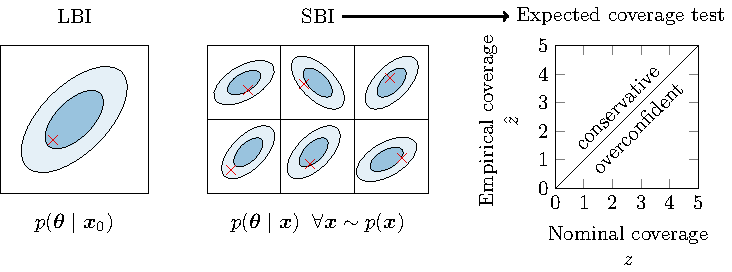
\includegraphics[width=\linewidth]{TikZ/sbi_test.pdf}
	\caption{Testability: Contrary to \gls*{lbi} algorithms, many \gls*{sbi} methods, including \gls*{tmnre}, do not estimate just a single posterior, but all of them simultaneously. This property is called ``amortization" in the machine learning field. Amortization enables the user to efficiently test the reliability of the inference results, for example with expected Bayesian coverage tests ({rightmost panel}). The left part of the figure is inspired and adapted from Figure 4 in Ref.~\cite{Cole:2021gwr}.
}
\label{fig:sbi-test}
\end{figure}


Using local amortization, one can cheaply validate the Bayesian coverage properties of the approximate posteriors \cite{Hermans:2021rqv, Cole:2021gwr, Karchev:2022xyn}, and construct confidence regions with exact frequentist coverage \cite{Karchev:2022xyn, dalmasso2020confidence, dalmasso2021likelihood}. Here we focus on the former types of tests, and use the \emph{expected coverage test} that probes the empirical (\ie~determined from analyses of simulated data $\data$) Bayesian coverage properties of the estimated posteriors $\hat{p}(\interest \mid \data)$.

An \emph{expected coverage test}  measures whether Bayesian credible regions of different widths have achieved their nominal coverage \cite{Hermans:2021rqv, Cole:2021gwr}. In simple words, it checks whether the true parameters $\interest$ fall within the $x\%$ credible region ($1-\alpha$) of the estimated posterior for $x\%$ of the randomly drawn observations $\data \sim p(\data\mid\interest)$. Agreement between the nominal and empirically-measured expected coverage is a necessary (but not sufficient) condition for the density/ratio estimator to be a correct estimate of the posterior. In case of a conservative estimator, the nominal credibility $1-\alpha$ is lower than the empirical one $1-\hat\alpha$, and vice versa for an overconfident estimator. In combination with visually checking the posteriors, this test supports the accuracy of the posterior estimator and is also particularly useful when one does not have access to the ground truth against which to compare the results.

Since we are mostly interested in small values of $\alpha$, corresponding to posterior regions with high mass, it is convenient to reparameterize $\alpha$ in terms of a new variable $z$, defined as $1-\frac12 \alpha$ quantile of the standard normal distribution \cite{Cole:2021gwr}. As a results,  $z = 1, 2, 3$ have $1-\alpha = 0.6827, 0.9545, 0.9997$, and correspond to the common $1\sigma$, $2\sigma$, $3\sigma$ regions. We show a mock example of such test in the right panel of in Figure~\ref{fig:sbi-test} to illustrate its general behaviour.

In Chapter~\ref{cha:lensing}, we will use empirical coverage plots in order to double-check and confirm the convergence of our posterior estimators for strong lensing image analysis. Closely related versions of this test and plots have appeared in the literature, \eg~in Refs.~\cite{Dax:2021tsq,Karchev:2022xyn, Bhardwaj:2023xph}. Developing more tests in order to trust results generated by \gls*{sbi} algorithms is very active and ongoing work. For example, it is worth mentioning an alternative method of defining Bayesian credible regions using distances to random points, which can, in certain circumstances, detect a systematic bias \cite{lemos2023sampling}.




\bigskip

\begin{figure}
	\centering
	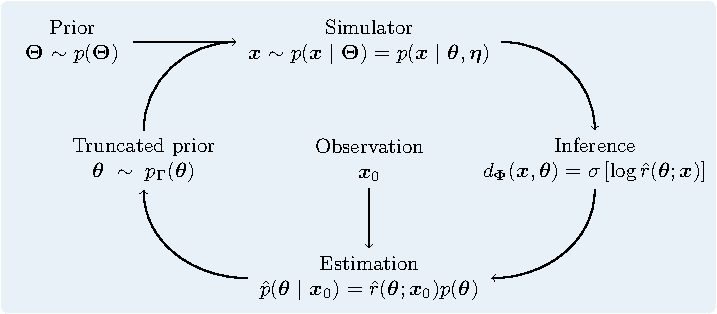
\includegraphics[width=\linewidth]{TikZ/tmnre.pdf}
	\caption{\textbf{Truncated marginal neural ratio estimation.} Parameters, both of interest $\interest$ and nuisance $\nuisance$, are sampled from the initial prior $p(\param)$, and mapped into data $\data$ through a programmed simulator that effectively acts as in implicit likelihood. Inference is performed by training binary classifiers $d_\Phi(\data, \interest)$ with marginal \gls*{nre} to learn the estimates of the ratios of interest $\hat{r}(\interest;\data)$ (Sections~\ref{subsec:tmnre-nre} and \ref{subsec:tmnre-m}). The ratios are used to weight prior samples, enabling posterior sampling for any observation $\data$. Focusing on a target observation $\data_0$, we can perform sequential inference (Section~\ref{subsec:tmnre-t}) via prior truncation, by constraining the initial parameter space for the inferred parameters to regions $\Gamma^{(R)}(\interest)$ that are most relevant for a specific target observation $\data_0$. The procedure is repeated until convergence.
}
	\label{fig:sbi-tmnre}
\end{figure}

In this section we have introduced the technical details of the \gls*{tmnre} algorithm, and its key building blocks: \gls*{nre} (Section~\ref{subsec:tmnre-nre}), marginalization  (Section~\ref{subsec:tmnre-m}), and prior truncation  (Section~\ref{subsec:tmnre-t}). We have also seen the general network architecture that is usually employed within this algorithm (Section~\ref{subsec:tmnre-nn}) and how to test its results (Section~\ref{subsec:tmnre-test}). A complete sketch of the workflow of a \gls*{tmnre} algorithm is illustrated in Figure~\ref{fig:sbi-tmnre}.


\section{SBI applications in this thesis} \label{sec:applications}

In this first chapter, we have learned about the benefits of simulation-based analysis for data inference, and particularly about the \gls*{tmnre} algorithm. In the next chapters, we will see its applications to various astrophysical problems: the analysis of strong gravitational lenses as a dark matter probe (Chapter~\ref{cha:lensing}), how to scale it to higher dimensional problems with more correlated parameter spaces (Chapter~\ref{cha:anre}), the reconstruction of cosmological initial conditions Chapter~\ref{cha:cosmo}), and the analysis of a population of point-sources in sky-maps (Chapter~\ref{cha:detection}). The common thread between all these applications is being formally representable by \emph{large and complex forward models}, with many moving parts, on a subpart of which we would like to perform precise scientific inference while correctly propagating uncertainties from the others. This is possible in a \gls*{sbi} framework.

In particular, we will see many of the several types of marginal posteriors that can be directly inferred in simulation-based settings, and which answer specific inference questions relevant for the application at hand. Some of the marginal quantities we will encounter in the different chapters of this thesis are:
\begin{itemize}[leftmargin=1cm]
	\item posterior of a single parameter (Chapters~\ref{cha:lensing}, \ref{cha:anre}, and \ref{cha:detection});
	\item 2-dimensional posteriors of parameter pairs (Chapters~\ref{cha:lensing}, \ref{cha:anre}, and \ref{cha:detection});
	\item n-dimensional posteriors of parameters (Chapter~\ref{cha:anre});
%	\item posterior for discrete (categorical) variables that label model choices
	\item posterior probability of a pixel value for field reconstruction (Chapter~\ref{cha:cosmo});
    \item posterior probability of an object being present in a specific image region (Chapter~\ref{cha:detection});
	\item posterior for the number of objects in an image  (Chapter~\ref{cha:lensing} and \ref{cha:detection}).
\end{itemize}


Moreover, prior truncation will be achieved by means of different strategies of increasing complexity throughout all of these applications, depending on the their specificities. The main strategies we will see are:
\begin{itemize}[leftmargin=1cm]
	\item 1-dimensional box truncation (Chapters~\ref{cha:lensing}, \ref{cha:anre}, and \ref{cha:detection});
	\item n-dimensional hard-likelihood truncation with nested sampling  (Chapter~\ref{cha:anre});
	\item truncation with tempered likelihood  (Chapter~\ref{cha:cosmo});
	\item object detection as prior truncation  (Chapter~\ref{cha:detection}).
\end{itemize}

A detailed contextualization and explanation of the technicalities of each strategy will be given in the respective chapters. 








%\chapter{Simulation-based inference for strong gravitational lensing} \label{cha:lensing}


Precision analysis of galaxy-galaxy strong gravitational lensing images provides a unique way of characterizing small-scale dark matter halos, and could allow us to uncover the fundamental properties of dark matter's constituents. Recently, gravitational imaging techniques made it possible to detect a few heavy subhalos. However, gravitational lenses contain numerous subhalos and line-of-sight halos, whose subtle imprint is extremely difficult to detect individually. Existing methods for marginalizing over this large population of sub-threshold perturbers to infer population-level parameters are typically computationally expensive, or require compressing observations into hand-crafted summary statistics, such as a power spectrum of residuals.

In this chapter, we present the first analysis pipeline to combine parametric lensing models and a recently-developed neural simulation-based inference technique called truncated marginal neural ratio estimation (\gls*{tmnre}) to constrain the warm dark matter halo mass function cutoff scale directly from multiple lensing images. Through a proof-of-concept application to simulated data, we show that our approach enables empirically testable inference of the dark matter cutoff mass through marginalization over a large population of realistic perturbers that would be undetectable on their own, and over lens and source parameters uncertainties. To obtain our results, we combine the signal contained in a set of images with Hubble Space Telescope resolution. Our results suggest that \gls*{tmnre} can be a powerful approach to put tight constraints on the mass of warm dark matter in the multi-keV regime, which will be relevant both for existing lensing data and in the large sample of lenses that will be delivered by near-future telescopes.



\section{Introduction} \label{sec:sl-intro}


\paragraph*{Dark matter puzzle.} Over the past several decades, numerous astrophysical probes including rotational curves of spiral galaxies \cite{Rubin:1980zd}, galaxy-cluster dynamics \cite{Zwicky:1933gu}, cosmic microwave background \cite{Planck:2015fie}, gravitational lensing observations \cite{Taylor:1998uk}, have established \gls*{dm} as one of the major components of the universe, comprising about $85\%$ of the its mass. However, up to the present time, the fundamental nature of \gls*{dm} is still one of the key unresolved puzzle in physics. For many years, the \gls*{cdm} paradigm has been able to accurately reproduce vastly disparate large-scale observations across all epochs. In this model, \gls*{dm} is massive, neutral, non-relativistic, and collisionless \cite{Peebles:1982ff}. %The main prediction of the \gls*{cdm} paradigm is that structure formation is due to a hierarchical clustering process, guided by gravitational instability of \gls*{dm} density perturbations, originated from quantum fluctuations during inflation. 

Despite providing a stunning description of the observed distribution of matter on large scales ($>\order{\si{\Mpc}}$), the agreement between \gls*{cdm} predictions and observations at galactic and sub-galactic scales has been less clear. At present, there is continued debate over whether the known abundance of dwarf galaxies and the density profiles of low-mass galaxies are in tension with the predictions of $\Lambda$CDM (respectively dubbed the missing satellites problem \cite{Moore:1999nt,Klypin:1999uc} and the cusp-core problem \cite{deBlok:1997zlw}, reviewed in Ref.~\cite{Bullock:2017xww}).
Solutions to these tensions include the impact of baryonic processes, such as supernovae feedback and reionization processes \cite{Bullock:2010uy}, or alternative \gls*{dm} physics. %Baryonic processes from supernovae feedback and reionization processes suppress star formation in low-mass galaxies \cite{Bullock:2010uy}, resulting in most \gls*{dm} subhalos not containing sufficiently bright galaxies and thus being more difficult to detect. Furthermore, baryonic feedback can "flatten out" the core of a dark matter profile, since feedback-driven gas outflows produce a time-varying gravitational potential that transfers energy to the orbits of the collisionless dark matter particles

The latter approach requires an alteration of \gls*{dm} particle physics, such that large-scale predictions remain unaffected, but the number of small-scale substructures is suppressed. \Gls*{dm} models which are warm instead of cold \cite{Colin:2000dn,Hogan:2000bv, Lovell:2013ola}, collisional instead of collisionless \cite{Spergel:1999mh}, or quantum on macroscopic scales rather than classical \cite{Hu:2000ke} predict a diverse array of possible configurations of low-mass halos and could potentially resolve these tensions \cite{Buckley:2017ijx}. Unfortunately, light \gls*{dm} halos are difficult to probe as they are not expected to accumulate enough baryonic matter to form stars and hence are truly \emph{dark} \cite{Efstathiou:1992zz,Fitts:2016usl}. If \gls*{dm} has significant self-interactions, such halos might be detectable by searching for the self-annihilation or decay products of \gls*{dm} \cite{Adhikari:2022sbh}. However, even if such interactions are not present, light halos can potentially be probed through their irreducible gravitational effects. In this chapter we study one such probe: galaxy-galaxy strong gravitational lensing.

\paragraph*{Strong gravitational lensing as a dark matter probe.} In strong gravitational lensing, the gravitational field of a mass distribution acts as a \emph{lens} by magnifying and distorting the light flux coming from a background \emph{source} \cite{Kochanek:aa}. This leads to multiple magnified and distorted images of the source, as explained by general relativity. The effect is sensitive only to how matter is distributed, regardless of its physical nature (baryonic/DM), and thus provides a direct way of probing the distribution of \gls*{dm} at small scales (see Ref.~\cite{Vegetti:2023mgp} for a recent review). 

% Hence, it provides a direct way of probing the distribution of \gls*{dm} at small scales, by means of the distortions to the images due to substructures on top of the main lens mass distribution. Therefore, gravitational lensing provides a pristine probe of small-scale structures and can in principle distinguish between \gls*{cdm} and \gls*{wdm} scenarios.


Indeed, a \emph{perturber} (\ie, a subhalo or \gls*{los} halo lying somewhere between the observer and source) positioned near one of these images contributes additional, much more localized distortions, on top of the main lens mass distribution. By carefully analyzing the relationship between the multiple images of the source, the distortions from dark perturbers can be disentangled from possible variations in the source light. Thus, a population of dark perturbers can collectively cause perturbations to images that can be detected statistically in order to constrain population-level parameters, such as the suppression scale in the the low-mass end of the \gls*{hmf}, which are dictated by the fundamental properties of \gls*{dm}. Therefore, gravitational lensing provides a pristine probe of small-scale structures and can in principle distinguish between \gls*{dm} scenarios.

\paragraph*{Strong lensing image analysis.} Various different methods have been suggested to analyse the effects of small-scale structures on lensing images \cite{Drlica-Wagner:2019aa}. These methods usually target two different types of lensing systems that differ in the lensed source: quadruply-lensed quasars, and extended background galaxies that get lensed into extended arcs or complete Einstein rings.

In the former case, the source is a nearly point-like quasar that is lensed into four compact images  (\emph{``quads''}). These images' positions and flux ratios comprise the summary statistics for these systems. The presence of a perturber near one of these images would cause anomalies in the ratios of their fluxes relative to what would be predicted assuming a smooth lens mass distribution. Evidence for flux ratio anomalies due to perturber was first found in Ref.~\cite{Mao:1997ek}. Later, Ref.~\cite{Dalal:2001fq} derived a statistical constraint on the substructure fraction in the lensing galaxies using a small sample of seven lensed quasars. Ref.~\cite{Nierenberg:2014cga} showed that flux-ratio anomalies can also be used to detect individual low-mass subhalos. Several studies derived upper limits on the subhalo mass function %half-mode mass $\mhm$
\cite{Nierenberg:2017vlg}, also including perturbations due to \gls*{los} halos \cite{Gilman:2017voy, Gilman:2019nap}. Further investigations pointed out the importance of correctly modeling baryonic structure in the main lens, in order to avoid systematic errors while constraining \gls*{dm} substructure abundance with flux-ratio anomalies \cite{Hsueh:2016aih, Hsueh:2017zfs, Hsueh:2019ynk}. 

Here we focus on \emph{gravitational imaging}, which refers to the analysis of lenses with extended arcs \cite{Koopmans:2005ig,Vegetti:2008eg,Vegetti:2009gw}. The observation in this case consists of a whole image. On one hand, such images cover a larger area of the sky than the four point-like images in quads, potentially providing more sensitivity to detect perturbations due to perturbers, in the form of percent-level variations in the shape of the predicted lensed light based on a smooth lens model. On the other hand, extracting this information requires modeling the source galaxy's light, which generally has a complex morphology. The gravitational imaging technique was first introduced in Ref.~\cite{Koopmans:2005nr} and further developed in Refs.~\cite{Vegetti:2008eg, Vegetti:2009gw}. Its application to real data has so far yielded to several detections of individual heavy ($>10^8 \si{\solmass}$) perturbers using deep, high-resolution observations in the optical from the \gls*{hst} and Keck as well as in radio data from Atacama Large Millimeter/sub-millimeter Array \cite{Vegetti:2010wa, Vegetti:2009cz, Vegetti:2012mc, Hezaveh:2016ltk,Diego:2022mii}. Moreover, measurements and non-detections of individual perturbers in samples of gravitational lens systems can be converted to constraints on the (sub)halo mass function and thus dark matter's properties \cite{Vegetti:2014lqa, Vegetti:2018dly,Ritondale:2018cvp}. 
% Moreover, samples of gravitational lens systems have been analyzed in \cite{Vegetti_2014, Vegetti_2018}, and, including \gls*{los} halos modeling, in \cite{Ritondale_2019}, in order to derive constraints on the \gls*{hmf} using detections and non-detections of individual substructures.

Established gravitational imaging analyses, such as the method in Refs.~\cite{Vegetti:2008eg,Hezaveh:2016ltk}, use \emph{likelihood-based} inference to infer the properties of perturbers. The central mathematical object in such approaches is the likelihood, a probabilistic model $p(\data \mid \param)$ for the data $\data$ given some parameters $\param$ for the lens, source, perturbers and possibly other (hyper)parameters.\footnote{For example, the hyperparameters could include the pixel size for pixelated sources or strength of source regularization.}   
Likelihood-based tools, such as \gls*{mcmc} or nested sampling~\cite{Skilling:2004pqw}, do not directly produce marginal posteriors but instead compute the \emph{joint posterior} $p(\param \mid \data_0)$, which must then be marginalized over. 

The computational expense of sampling from the high-dimensional joint posterior imposes restrictions on the realism of lensing models that can be analyzed. One such restriction common to most analyses is to  assume a particular form of the noise and source model so that the source uncertainties can be excluded from the sampling and marginalized over analytically \cite{Hezaveh:2016ltk,Vegetti:2008eg,Vegetti:2009cz,Vegetti:2010wa,Vegetti:2012mc}. This makes it difficult to explore more complex source models described by \eg~generative machine learning methods or noise artifacts like cosmic ray streaks that cannot be described by an analytic likelihood.

An additional difficulty with likelihood-based analyses is that each run of \gls*{mcmc} or nested sampling produces posterior samples for just a single observation. Directly exploring the systematics, biases and other statistical properties of a particular lensing model is thus extremely time-consuming, necessitating rerunning posterior sampling many times for different input observations. This also makes analyses such as mapping perturber measurement sensitivity costly. It is noteworthy that recently Ref.~\cite{Nightingale:2022bhh} pushed to the limits how far one can feasibly go using likelihood-based analyses, fitting 54 images with 5 different mass models.

Likelihood-based analyses also typically assume no more than two perturbers are present in each image. Allowing for $n$ perturbers would cause the joint posterior to become highly multimodal, with approximately $n!$ modes due exact invariance of the observation under relabeling of perturbers. In these frameworks, it is then challenging to perform statistical inference of quantities such as the posterior for substructure population-level parameter of interest, marginalizing over all source, lens, and substructures parameters to get the marginal of interest.

%In reality, constraining collective substructure properties from gravitational lensing images is an extremely difficult problem. In fact, inferring marginal posteriors for the \gls*{hmf} cutoff requires marginalizing over all source, lens, and substructures parameters to get the marginal likelihood for the population-level parameter of interest, thus involving a time-consuming exploration of a very high-dimensional parameter space for complex realistic models. Therefore, \gls*{mcmc} or nested sampling methods would imply an intractable sampling from the high-dimensional joint posterior. 


\emph{Transdimensional Bayesian inference} partially overcomes this traditional likelihood-based methods' challenge, by using transdimensional \gls*{mcmc} to infer the probabilities of different possible populations of perturbers, albeit at substantial computational cost \cite{Brewer:2015yya,Daylan:2017kfh}. 

An alternative strategy involves linearizing the gravitational potential via a \emph{Taylor expansion} of the lens equation. By employing a Taylor expansion, it becomes feasible to capture all small-scales \gls*{dm} substructures without the need to parameterize them directly in the likelihood function \cite{Vegetti:2008eg, Koopmans:2005nr, Galan:2022ifd}. This technique is therefore able to account for the full \gls*{dm} subhalo population (a part from the effects due to the curl-component induced by multi-plane lensing effects).

Another viable approach to reduce the dimensionality of the problem and enable inference of the collective effects of a large number of low-mass substructures at the statistical level requires engineering \emph{summary statistics} from first principles, such as the convergence \gls*{ps} for different subhalo populations \cite{DiazRivero:2017xkd, DiazRivero:2018aa, Brennan:2018jhq}, and also for \gls*{los} populations \cite{CaganSengul:2020nat}. However, this approach is not directly applicable to observations, because we do not have access to the true displacement field from the data. Building upon this, it is possible to relate the \gls*{ps} of the surface brightness fluctuations in strong lens images to the lens potential fluctuations arising from \gls*{dm} distribution that contribute to the convergence \gls*{ps} \cite{Chatterjee:2017orx, Cyr-Racine:2019aa, Bayer:2018vhy}. Another summary statistic that has been employed is the residuals between the image and best-fit reconstruction excluding substructure, that is related to the (sub)halo mass function parameters. In particular, this summary statistic has been successfully employed to constrain the \gls*{hmf} suppression scale using \gls*{abc} \cite{Birrer:2017rpp, He:2020rkj}, a likelihood-free inference method based on a rejection algorithm, as seen in Section~\ref{sec:sbi}. This approach reduces the dimensionality of the problem and enable inference of the collective effects of a large number of low-mass substructures at the statistical level. However, it is unknown how much information such approach discards. 

Another class of methods that has developed in recent years uses \emph{neural networks} to measure lens parameters \cite{Hezaveh:2017sht, PerreaultLevasseur:2017ltk,  Morningstar:2019szx}, quantifying the structure of gravitational lens potential \cite{Vernardos:2020aa}, detect individual subhalos \cite{Rivero:2020aa}, distinguish different types of \gls*{dm} substructure based on their lensing signatures \cite{Alexander:2019puy}, and classify whether each pixel in an image contained a subhalo in a given mass bin \cite{Ostdiek:2020cqz,Ostdiek:2020mvo}. Still, these methods need lots of data to amortize over all possible variations in lensing systems. In fact, amortized methods learn the posterior for any data, generated by any parameter over the whole range of the prior. But learning an amortized posterior is unnecessary if only a small range of parameters are consistent with a target observation.
 

\paragraph*{This work.} In this work, we demonstrate that a \gls*{sbi} \cite{Cranmer:2019eaq} method called truncated marginal neural ratio estimation \cite{Miller:2020hua,Miller:2021aa}, from here on \gls*{tmnre}, can circumvent the inference challenges discussed in the above paragraphs. 
In particular, we use strong gravitational lensing to constrain \gls*{wdm} models \cite{Colin:2000dn, Lovell:2013ola}, which are well-motivated from a particle physics perspective (see \eg~sterile neutrinos \cite{Boyarsky:2018tvu} and gravitinos \cite{Bond:1982uy}). In \gls*{wdm} models \gls*{dm} particles have non-negligible thermal velocities that allow them to free-stream out of density perturbations, effectively preventing small-scale structure formation. The scale at which this happens depends on model parameters and is parametrised by the half-mode mass, $\mhm$, in the \gls*{hmf}. Therefore, one of the viable way to discriminate between \gls*{cdm} and alternative \gls*{wdm} models is to constrain the low-mass end of the \gls*{hmf} by probing small-scale \gls*{dm} halos which are completely devoid of stars and truly \emph{dark}, whose only signature is then gravitational. 

Here, we present the first analysis pipeline that combines parametric lensing models with recent \gls*{tmnre} developments to infer the half-mode mass $\mhm$ of the subhalo \gls*{hmf} directly from images by combining a set of realistic simulated galaxy-galaxy strong lenses, 
%to \emph{measure the suppression scale of the subhalo \gls*{hmf} directly from images by combining multiple observations}.  
In fact, there are currently around a hundred strong lensing observations suitable for substructure inference, most of which come from the SLACS \cite{Bolton:2005nf} and BELLS \cite{BOSS:2011bef} surveys. In the near future, new and future telescopes like JWST \cite{Gardner:2006ky}, ELT \cite{Simon:2019aa}, Euclid \cite{Refregier:2010ss, EUCLID:2011zbd}, SKA \cite{Koopmans:2004gf}, and LSST \cite{LSSTDarkEnergyScience:2020oya} will greatly increase the quality of data suitable for gravitational imaging analyses as well as its quantity, from $\order{100}$ to $\order{10^5}$ images \cite{Collett:2015roa, McKean:2015aa}. It is then extremely important to be able to combine the information coming from different observations in the statistical analysis.

%For the statistical analysis we employ \gls*{tmnre}. Developed by Ref.~\cite{Hermans:2019ioj} and Ref.~\cite{Miller:2020hua}, \gls*{mnre} is a neural \gls*{sbi} method that makes it possible to learn the marginal posterior approximation for a specified subset of model parameters of interest directly from the full input data that, in our case, corresponds to the observed lensed images, without the need for hand-crafted summary statistics. This method improves the simulator efficiency and the quality of inference. Moreover, \gls*{mnre} is amortized, which  enables important statistical consistency tests, which would have been extremely expensive with likelihood-based inference, like the expected coverage test we employ in Section~\ref{subsec:test}. 
As discussed in Chapter~\ref{cha:sbi}, \gls*{sbi} refers to a class of statistical inference methods that use the output of a stochastic simulator that need not have a known likelihood. In particular, \gls*{nre}, first presented in \cite{Hermans:2019ioj}, trains a neural network to map from observations directly to \emph{marginal posteriors} for a specified subset of model parameters (\eg~the Einstein radius of a lens). This bypasses the requirement of likelihood-based inference to sample the joint posterior. In contrast to methods like \gls*{abc}, this also removes the need to engineer summary statistics \cite{He:2020rkj} as they are in effect learned directly from the training data. Since \gls*{nre} learns a marginal posterior \emph{function}, it is straightforward to check the statistical properties of the inference results for different observations. \gls*{tmnre} further extends \gls*{nre} by focusing training data generation in the regions of parameter space most relevant for analyzing a particular observation over a sequence of inference rounds. This substantially reduces the number of simulations required to train the inference network as well as the required network complexity. This truncation method applied to strong-lensing images was proposed in Ref.~\cite{Karchev:2021fro} and used in Ref.~\cite{Coogan:2020yux} to learn marginal posterior approximations for individual subhalo parameters, marginalizing over lens and source uncertainties given an observation.

Several other works have applied \gls*{sbi} to substructure lensing. In Ref.~\cite{Zhang:2022djp} a likelihood-ratio estimation technique similar to \gls*{tmnre} was employed to measure density profile parameters of subhalos from images. Ref.~\cite{Wagner-Carena:2022mrn} recently applied neural posterior estimation to measure the subhalo \gls*{hmf} normalization in mock lensing images using real galaxy images as sources. Ref.~\cite{Brehmer:2019jyt} utilized a ``likelihood-based'' \gls*{sbi} method requiring the simulator's score\footnote{
    The score is the derivative of the log-likelihood for a given observation with respect to the model's parameters.
} to measure the slope and normalization of a subhalo \gls*{hmf} in simple mock images.
%Up to now, this approach has been applied in simplified modeling frameworks: Ref.~\cite{Hermans:2019ioj} focuses on recovering the Einstein radius of a gravitational lens marginalizing over 15 source and lens mass distribution parameters, whereas Ref.~\cite{Brehmer:2019jyt} estimates the slope and normalization of a \gls*{cdm} subhalo mass function. \gls*{sbi} using neural posterior density estimator and hierarchical inference have also been employed in Ref.~\cite{Wagner-Carena:2022mrn} to infer the \gls*{cdm} subhalo mass function normalization from a set of strong-lensing images, generated using real galaxy images as a source model, including realistic observational noise effects from \gls*{hst} and accounting for the mean expected convergence from \gls*{los} halos. 

The present work complements these efforts in several ways. First, it demonstrates that our \emph{hierarchical} \gls*{tmnre} approach is able to efficiently and accurately infer the statistic of the \gls*{hmf} suppression scale given a set of \gls*{hst} resolution observation. Then, it illustrates the importance of combining the information coming from different observations in the statistical analysis, especially in light of near-future data delivery. Lastly, it shows that \gls*{tmnre} enables statistical checks that would be extremely expensive with likelihood-based inference since they would require rerunning the sampling machinery on numerous mock observations.

This chapter is organized as follows. In Section~\ref{sec:sl-model} we describe our strong lensing model, which uses an analytic source and main lens in conjunction with a well-motivated perturber model that accounts for both subhalos and \gls*{los} halos. In Section~\ref{sec:sl-analysis} we briefly discuss the inference methodology based on \gls*{tmnre} employed in the statistical analysis. Then, we show our results for hierarchical inference of the halo mass function suppression scale from an ensemble of lenses in Section~\ref{sec:sl-results}. Finally, we conclude in Section~\ref{sec:sl-conclusions}. 
This work will help form the basis for \gls*{sbi}-based analysis of strong lensing images as a dark matter probe in existing and future lensing data.




\section{Modeling strong lensing observations}  \label{sec:sl-model}

Here we review how we model strong lensing images. We implement our lensing model in \texttt{PyTorch} \cite{pytorch} so that we can leverage GPUs to rapidly generate large numbers of observational data (a single-channel telescope image).

\subsection{The physics of strong lensing}
Before delving into modeling details, we briefly summarize the key points of the physics of gravitational lensing, referring the reader to \eg~Ref.~\cite{Meneghetti:2016aa} for a more detailed overview. In strong-lensing systems the mass distribution of a foreground galaxy gravitationally lenses the light rays coming from a background source, resulting in an arc-like image in the case of an extended galaxy source. We assume that mass densities are low enough to treat the gravitational field of the matter in the image plane in the Newtonian approximation of \gls*{gr}. In this case the metric is fully characterized by the lens' gravitational potential $\psi$. We also adopt the thin lens approximation, which assumes all the lens mass lies in a single \emph{image plane} and all the source light is emitted from a \emph{source plane}. 

We will be using $\vec{\xi}\equiv(\xi_x, \xi_y)$ and $\vec{x}\equiv(x, y)$ as two-dimensional angular coordinates in the image and source planes respectively, and use $z$ to indicate distances along the orthogonal dimension. Since the image plane covers a small angular patch of the sky and the lensing deflections are small in the Newtonian limit, the coordinate system can be treated as Cartesian.

The configuration, then, is determined by two fields: the distribution of surface brightness in the source plane, $\beta(\vec{x})$, and the distribution of mass in the image plane, described by the projected potential:
\begin{equation}
	\Psi(\vec{\xi})\equiv \int_{-\infty}^{\infty} \psi(\xi_x, \xi_y, z) \mathrm{d}z
\end{equation}

Under these assumptions, the source-plane coordinate to which a light ray through the image plane traces back is given by the simple \emph{lens equation}
\begin{equation} \label{eq:gl-lensing}
    \vec{x} = \vec{\xi} - \vec{\alpha}(\vec{\xi}) \, .
\end{equation}
The displacement field $\vec\alpha$ is determined by the projected potential:
\begin{equation} \label{eq:disp_grad}
    \vec{\alpha}(\vec{\xi}) = \frac{D_{LS}}{D_S} \frac{2}{c^2} \frac{\vec{\nabla}_{\vec{\xi}} \Psi(\vec\xi)}{D_L} \, ,
\end{equation}
where the gradient is taken in the image plane and should have dimensions of inverse length, whence the introduction of the observer-lens angular diameter distance $D_L$. The expression also involves the angular diameter distances $D_{LS}$ (from the lens to the source), and $D_S$ (from the observer to the source).\footnote{
    We compute angular diameter distances with \texttt{astropy}~\cite{Astropy:2013muo,Astropy:2018wqo} using the flat cosmology from Planck \cite{Planck:2018vyg}.
} 
We illustrate in Figure~\ref{fig:gl-lensing} the geometry of the system.

\begin{figure*}
    \centering
    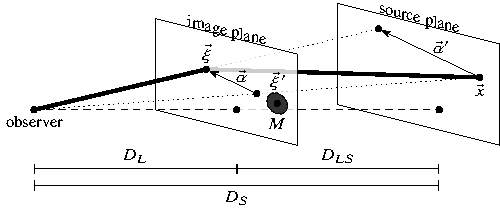
\includegraphics[width=0.8\linewidth]{Figures/GL-lensing.pdf}
    \caption{Thin lens geometry. The lensing mass $M$ located at $\vec\xi'$ bends the light ray (thick line) emanating from the point $\vec x$, so that to the observer it looks like it is coming from the direction of $\vec\xi$ . General relativity predicts the deflection angle $\vec\alpha'$  \emph{as viewed from the image plane} based on the mass $M$ and the impact parameter $\vec b = \vec \xi - \vec \xi '$. It then has to be rescaled by $\frac{D_{LS}}{D_S}$ to obtain the displacement field $\vec\alpha$ (as viewed by the observer) for use in Equation~\eqref{eq:gl-lensing}. Angles are all assumed to be small enough that they can be used for Euclidean calculations. The dashed line is the optical axis perpendicular to the planes and connects the origins of the coordinate systems for each plane. The figure is a reproduction of Figure 2 in Ref.~\cite{Karchev:2021fro}.}
    \label{fig:gl-lensing}
\end{figure*}

From a computational standpoint it is more convenient to represent Equation~\eqref{eq:disp_grad} as an integral. Using the Poisson equation $\nabla_2 \Psi= 4\pi G\rho$ and setting appropriate boundary conditions:
\begin{equation} \label{eq:disp_int}
    \vec{\alpha}(\vec{\xi}) = \frac{4 G}{c^2} \frac{D_{LS}}{D_L \, D_S} \int \Sigma(\vec{\xi}') \frac{\vec{\xi} - \vec{\xi}'}{\mid\vec{\xi} - \vec{\xi}'\mid^2}   \mathrm{d}{(D_L \vec{\xi}')} \, ,
\end{equation}
where the integral is performed over the image plane, and where $c$ is the speed of light and $G$ is the gravitational constant.

Here $\Sigma$ is the projected (surface) mass density related to the 3D mass density $\rho$ by an integration along the coordinate perpendicular to the lens plane $z$:
\begin{equation}
	\Sigma(\vec\xi) \equiv \int_{-\infty}^{\infty} \rho({\xi}_x, {\xi}_y, z) \mathrm{d}{z},
\end{equation}
similarly to the expression for the projected potential.

The expression in Equation~\eqref{eq:disp_int} can be simplified by introducing the convergence $\kappa$ in terms of the critical surface density $\Sigma_{\mathrm{cr}}$:
\begin{equation}
    \kappa(\vec{\xi})=\cfrac{\Sigma(\vec{\xi})}{\Sigma_{\mathrm{cr}}},
    \quad \Sigma_{\mathrm{cr}}\equiv\cfrac{c^2}{4\pi G}\cfrac{D_S}{D_L D_{LS}} \, .
\end{equation}
If  $\kappa > 1$, a lens can form multiple images \cite[Section 2.6]{Meneghetti:2016aa}. The threshold for this to happen is set by the critical surface density, and it is evident from its expression that for a fixed distance to the lens ($D_L $) further away sources  ($D_S$) are lensed more easily, since they require smaller deflections.

Furthermore, it can be shown that the convergence $\kappa$ is related to the isotropic part of the trace of the Jacobian of the lensing transformation through
\begin{equation}\label{eq:lens-jacobian}
	\frac{\dd{\vec{x}}}{\dd{\vec{\xi}}} = \mqty(\dmat[0]{1-\kappa, 1-\kappa}) - \mqty(\gamma_1 & \gamma_2 \\ \gamma_2 & -\gamma_1),
\end{equation}
where the second part is the shear (discussed more in details in Section~\ref{subsec:sl-model-lens}).
Another important quantity is the inverse of the Jacobian's determinant, the magnification
\begin{equation}
	\mathcal{M} \equiv \mid\frac{\dd{\vec{\xi}}}{\dd{\vec{x}}}\mid  = \qty[(1-\kappa)^2 - \qty(\gamma_1^2 + \gamma_2^2)]^{-1},
\end{equation}
which is a measure of how much the solid angle spanned by the source is enlarged, or equivalently, of how gravitational focusing directs a larger fraction of the energy radiated by the source to the observer \cite{Bartelmann:1999yn}. Thus, when the convergence $\kappa$ and the shear $\gamma$ are equal or greater than unity, sources are \emph{strongly} magnified, and we can use the magnitude of the magnification to differentiate between \emph{strong} from \emph{weak} lensing regimes.

While lensing does change the apparent solid angle of a source, it is worth noting that it conserves energy, since it merely alters the trajectories of photons rather than creating or destroying them. As a result, the surface brightness $\beta(\vec{\xi})$ in the image plane is equal to the surface brightness at the point to which it traces back in the source plane (assuming one isolated source):
\begin{equation}
    \beta(\vec{\xi}) = \beta(\vec{x}(\vec{\xi})) \, .
\end{equation}

%It is important to note, however, that lensing does not create or destroy photons (and thus, conserves energy.}). Thus, the amount of light arriving at the observer is proportional to the area \emph{in the image plane} that the source subtends, which effectively acts as a collecting area for light that is then simply rerouted just as with conventional lenses. This means that \emph{lensing conserves surface brightness} around infinitesimal points, and thus the surface brightness registered by the observer (in the absence of other sources) is
%\begin{eq}
%	\sbr(\ximg) = \sbr(\x\qty(\ximg)).
%\end{eq}
%
%It is obvious from this expression that the lens and the source are entirely degenerate: for any observation there is for every deflection field (that does not form multiple images!) a surface brightness configuration that can reproduce the observation. The reverse (that one can find deflection fields that map distinct sources to the same image) is also sometimes true, giving rise to the mass-sheet \cite{masssheetdegeneracy} and source-position degeneracies \cite{sourcepositiontransformation} (the latter being more general but approximate). As a consequence, the spatial scale of the source cannot be conclusively determined (in the absence of time-delay data \ered{or additional constrants on the lens mass profile}) since a sheet of constant mass density could be magnifying it uniformly by an arbitrary amount \cite{lensing-short}.


\bigskip

Given the physics of strong lensing, in order to fully specify a strong-lensing model we then need two main ingredients: the lens model, which describes the total mass distribution of the lens, and the source model, which describes the surface brightness profile of the background source. It is common to split the lens model into a macroscopic smooth component (main lens and external shear) and a substructure\footnote{Throughout this thesis, we use the terms `small-scale structures', `substructures', and `low-mass halos' when considering both subhalos of the main lens and line-of-sight halos.} component, due to subhalos and line-of-sight halos. Each lensing ingredient can be directly superimposed by summing their respective displacement fields in the lens plane:
\begin{equation}
    \vec{\alpha} = \vec{\alpha}_\mathrm{lens} + \vec{\alpha}_\mathrm{ext} + \sum_{i=1}^{N_{\mathrm{sub}}} \vec{\alpha}_\mathrm{sub,i} + \sum_{i=1}^{N_{\mathrm{los}}} \vec{\alpha}_\mathrm{los,i}.
\end{equation}
In the following sections, we will describe each component of the model we use to simulate mock images of gravitational lenses: the source, the main lens, the dark matter perturbers, and instrumental noise. The model and its priors are summarized in Table~\ref{tab:pop-model}.

\begin{table}
\begin{center}
\resizebox{0.9\columnwidth}{!}{%
    \begin{tabular}{l l l c }
        \toprule
        Parameter & {True value} & Prior & Description \\
        \midrule
        \textbf{Main lens} &  &  &  SPLE \\
        $\theta_E$ [\si{\arcsecond}] &  & $\Uniform(1.,2.)$  & Einstein radius \\
        $\xi_{0,x}$ [\si{\arcsecond}] &  & $\Uniform(-0.2,0.2)$  & lens center x axis \\
        $\xi_{0,y}$ [\si{\arcsecond}] &  & $\Uniform(-0.2,0.2)$  & lens center y axis \\
        $q_l$ &  & $\Uniform(0.1,1.)$ & axis ratio \\
        $\phi_l$ [\si{\radian}]&  & $\Uniform(0,2\pi)$  & rotation angle \\
        $\gamma$ & 2.1 & -  & slope \\
        $z_\mathrm{lens}$ & 0.5 & -  & lens redshift \\
        \midrule
        \textbf{External shear}  &  &  &   \\
        $\gamma_1$ &  & $\Uniform(-0.05,0.05)$  & $1^{\mathrm{st}}$ component\\
        $\gamma_2$ &  & $\Uniform(-0.05,0.05)$   & $2^{\mathrm{nd}}$ component\\
        \midrule
        \textbf{Source} &  &  &  Sérsic \\
        $I_e$ &  & $\Uniform(0.,4.)$  & surface intensity \\
        $r_e$ [\si{\arcsecond}] &  &  $\Uniform(0.1,2.5)$ & effective radius \\
        $x_0$ [\si{\arcsecond}] &  & $\Uniform(-0.1,0.1)$ & source center x axis\\
        $y_0$ [\si{\arcsecond}] &  & $\Uniform(-0.1,0.1)$ & source center y axis\\
        $q_s$ &  & $\Uniform(0.1,1.)$ & axis ratio\\
        $\phi_s$ [\si{\radian}] &  &  $\Uniform(0,2\pi)$  & position angle\\
        $n$&  &  $\Uniform(0.1,4.)$  & index\\
        $z_\mathrm{src}$ & 2 & -  & source redshift\\
        \midrule
        \textbf{Subhalos} & & &  tNFW \\
        $\vec{p}$ [\si{\arcsecond}] & {$\in[-2.5, 2.5]$} & $\Uniform_{2\mathrm{D}}(-2.5, 2.5)$ & position\\
        $m_{200}$ [\si{\solmass}] & {$\in[10^7, 10^{10}]$} & \cite{Giocoli:2009ie} & virial mass\\
        $c_{200}$ & 15. & - & concentration \\
        $\tau$ & 6. & - & truncation\\
        \midrule
        \textbf{\gls*{los} halos} &  &  &  projected tNFW \\
        $\vec{p}$ [\si{\arcsecond}] & {$\in[-2.5, 2.5]$} & $\Uniform_{2\mathrm{D}}(-2.5, 2.5)$ & position\\
        $m_{200}$ [\si{\solmass}] & {$\in[10^7, 10^{10}]$} & \cite{Tinker:2008ff} & virial mass\\
        $z_{\mathrm{LOS}}$ & {$\in[0, z_\mathrm{src}]$} &  \cite{Tinker:2008ff} & LOS redshift\\
        $c_{200}$ & 15. & - & concentration \\
        $\tau$ & 6. & - & truncation\\
        \midrule
        \textbf{\gls*{wdm}} &  & &  \\
        $\mhm$ [\si{\solmass}] & & $\log\Uniform(10^7, 10^{10})$ & half-mode mass\\
        \bottomrule
    \end{tabular}
}
\end{center}
\caption{Summary of model parameters used for the simulated images in this work. When a prior distribution is not specified, the parameter is fixed to the true value.}
\label{tab:pop-model}
\end{table}



\subsection{Source model} \label{subsec:source}
To model the surface brightness of the source galaxy, we adopt the widely-used Sérsic profile \cite{Sersic:1963aa}. The surface brightness distribution is parameterized by 
\begin{equation}\label{eq:sersic}
    \beta(\vec{x})=I_e \exp{-k_n\left[\left(\cfrac{R(\vec{x})}{r_e}\right)^{1/n}-1\right]},
\end{equation}
where $I_e$ is the surface intensity at the half-light radius $r_e$. The radial parameter $r(\vec{x})=\sqrt{r_x^2+r_y^2}$ is the length of the elliptical radial coordinate vector
\begin{equation}
    \begin{pmatrix} 
        r_x \\ r_y 
    \end{pmatrix} = 
    \begin{pmatrix} 
      \sqrt{q_s} & 0 \\ 0 & 1/\sqrt{q_s} 
    \end{pmatrix} 
    \begin{pmatrix} 
        \cos\phi_s & \sin\phi_s \\ -\sin\phi_s & \cos\phi_s 
    \end{pmatrix} 
    \begin{pmatrix} 
        x - x_{0,s} \\ y - y_{0,s} 
    \end{pmatrix},
\end{equation}
which depends on the source's position angle $\phi_s$, axis ratio $q_s$, and center of light position $(x_{0,s}, y_{0,s})$. 

The normalization $k_n$ is related to the index $n$ by an implicit transcendental equation in terms of the complete and lower incomplete gamma functions $2\gamma(2n, k_n)=\Gamma(2n)$. We use the expansion in series from Ref.~\cite{Ciotti:1999zs}, 
\begin{equation}
    k_n \approx 2 n - \frac{1}{3} + \frac{4}{405 n} + \frac{46}{25515 n^2} + \frac{131}{1148175 n^3} - \frac{2194697}{30690717750 n^4} \, .
\end{equation}
valid over a wide range of indices, $n>0.36$. For typical galaxies $1/2 < n < 10$.

Therefore, our source model is parametrised by seven variables that we collect in the vector $\psrc \equiv\{I_e, r_e, x_{0,s}, y_{0,s}, q_s, \phi_s, n\}$. We fix the source's redshift to $z_\mathrm{source} = 2$.

\subsection{Main lens model}\label{subsec:sl-model-lens}

%\footnote{
%    Throughout our work,  we use the terms “simulated data” for data used during inference and “mock observations” for the simulated data that we analyze.
%    }     
    
We adopt the \gls*{sple} model for the main lens galaxy, which is capable of modeling the gravitational potentials of strong lenses to near the percent level~\cite{Suyu:2008zp}. Furthermore, the \gls*{sple} model has been shown to be a more adequate representation of the combined \gls*{dm} and baryon mass distribution in the inner regions of galaxies, to which strong lensing is most sensitive \cite{Suyu:2008zp}. The \gls*{sple} deflection field can be expressed in closed-form as a complex field $\alpha = \alpha_x + i \alpha_y$ \cite{Tessore:2015baa,ORiordan:2020aa}:
\begin{equation}
\begin{split}
    \vec{\alpha}^\mathrm{SPLE}(\vec{\xi}) = \theta_E & \frac{2 q_\mathrm{l}^{1/2}}{1 + q_\mathrm{l}} \left( \frac{\theta_E}{r} \right)^{\gamma - 2} e^{i \varphi} \\
    & \cdot \hypgeom\left( 1, \frac{\gamma - 1}{2}, \frac{5 - \gamma}{2}, -\frac{1-q_\mathrm{l}}{1+q_\mathrm{l}} e^{2 i \varphi} \right) \, .
\end{split}
\end{equation}
Here $(r, \varphi)$ are elliptical coordinates, related to the Cartesian coordinates $\vec{\xi}$ through a transformation parametrized by the lens' orientation $\phi_\mathrm{l}$, axis ratio $q_\mathrm{l}$ and position $(\xi_\mathrm{x, 0}, \xi_\mathrm{y, 0})$:
\begin{align}
    \begin{pmatrix} r_x \\ r_y \end{pmatrix} &= \begin{pmatrix} q_\mathrm{l}^{1/2} & 0 \\ 0 & q_\mathrm{l}^{-1/2} \end{pmatrix} \begin{pmatrix} \cos\phi_\mathrm{l} & \sin\phi_\mathrm{l} \\ -\sin\phi_\mathrm{l} & \cos\phi_\mathrm{l} \end{pmatrix} \begin{pmatrix} \xi_x - \xi_{x, 0} \\ \xi_y - \xi_{y, 0} \end{pmatrix} \, ,\\
    \tan \varphi &= \frac{r_y}{r_x}.
\end{align}

In the circular ($q=1$) isothermal ($\gamma=2$) case this reduces to $\alpha=\theta_E e^{i\varphi}$, \ie~is an isotropic constant, as is well-known. Since the hypergeometric function $\hypgeom$, however, is not implemented in \texttt{PyTorch}, we instead pretabulate its value as a function of $\phi_\mathrm{l}$, $q_\mathrm{l}$ and $\gamma$ and interpolate at runtime, as described in Ref.~\cite{Chianese:2019ifk}. This results in very fast code with negligible output degradation.

The slope $\gamma$ has a complicated degeneracy with the size of the source \cite{Schneider:2013sxa,Schneider:2013wga}. Roughly, larger $\gamma$ values cause the spatial scale of the source to increase \cite[Section 3.3]{Nightingale:2014aa}. For simplicity we fix $\gamma = 2.1$. In principle, inferring the slope is possible, but it requires more training data and leads to increased uncertainties in both lens and source parameters.

We also assume the lens galaxy's light has been perfectly subtracted, and fix its redshift to $z_\mathrm{lens} = 0.5$.

To account for the weak lensing due to large-scale structure located along the line of sight to the source, we also include an external shear component, which is constant across the image plane:
\begin{equation}
    \vec{\alpha}^\mathrm{shear}(\vec{\xi}) = \begin{pmatrix} \gamma_1 & \gamma_2 \\ \gamma_2 & -\gamma_1 \end{pmatrix} \vec{\xi} \, .
\end{equation}

Our main lens model thus has seven parameters: the \gls*{sple} parameters $(\xi_{x, 0}, \xi_{y, 0}, \phi_\mathrm{l}, q_\mathrm{l}, \theta_E)$ and the external shear parameters $(\gamma_1, \gamma_2)$, which we denote collectively with $\plens$.

\subsection{Small-scale structures model} \label{subsec:substructure}

\begin{figure}
	\centering
	\begin{subfigure}[b]{0.5\linewidth}  
	\centering
	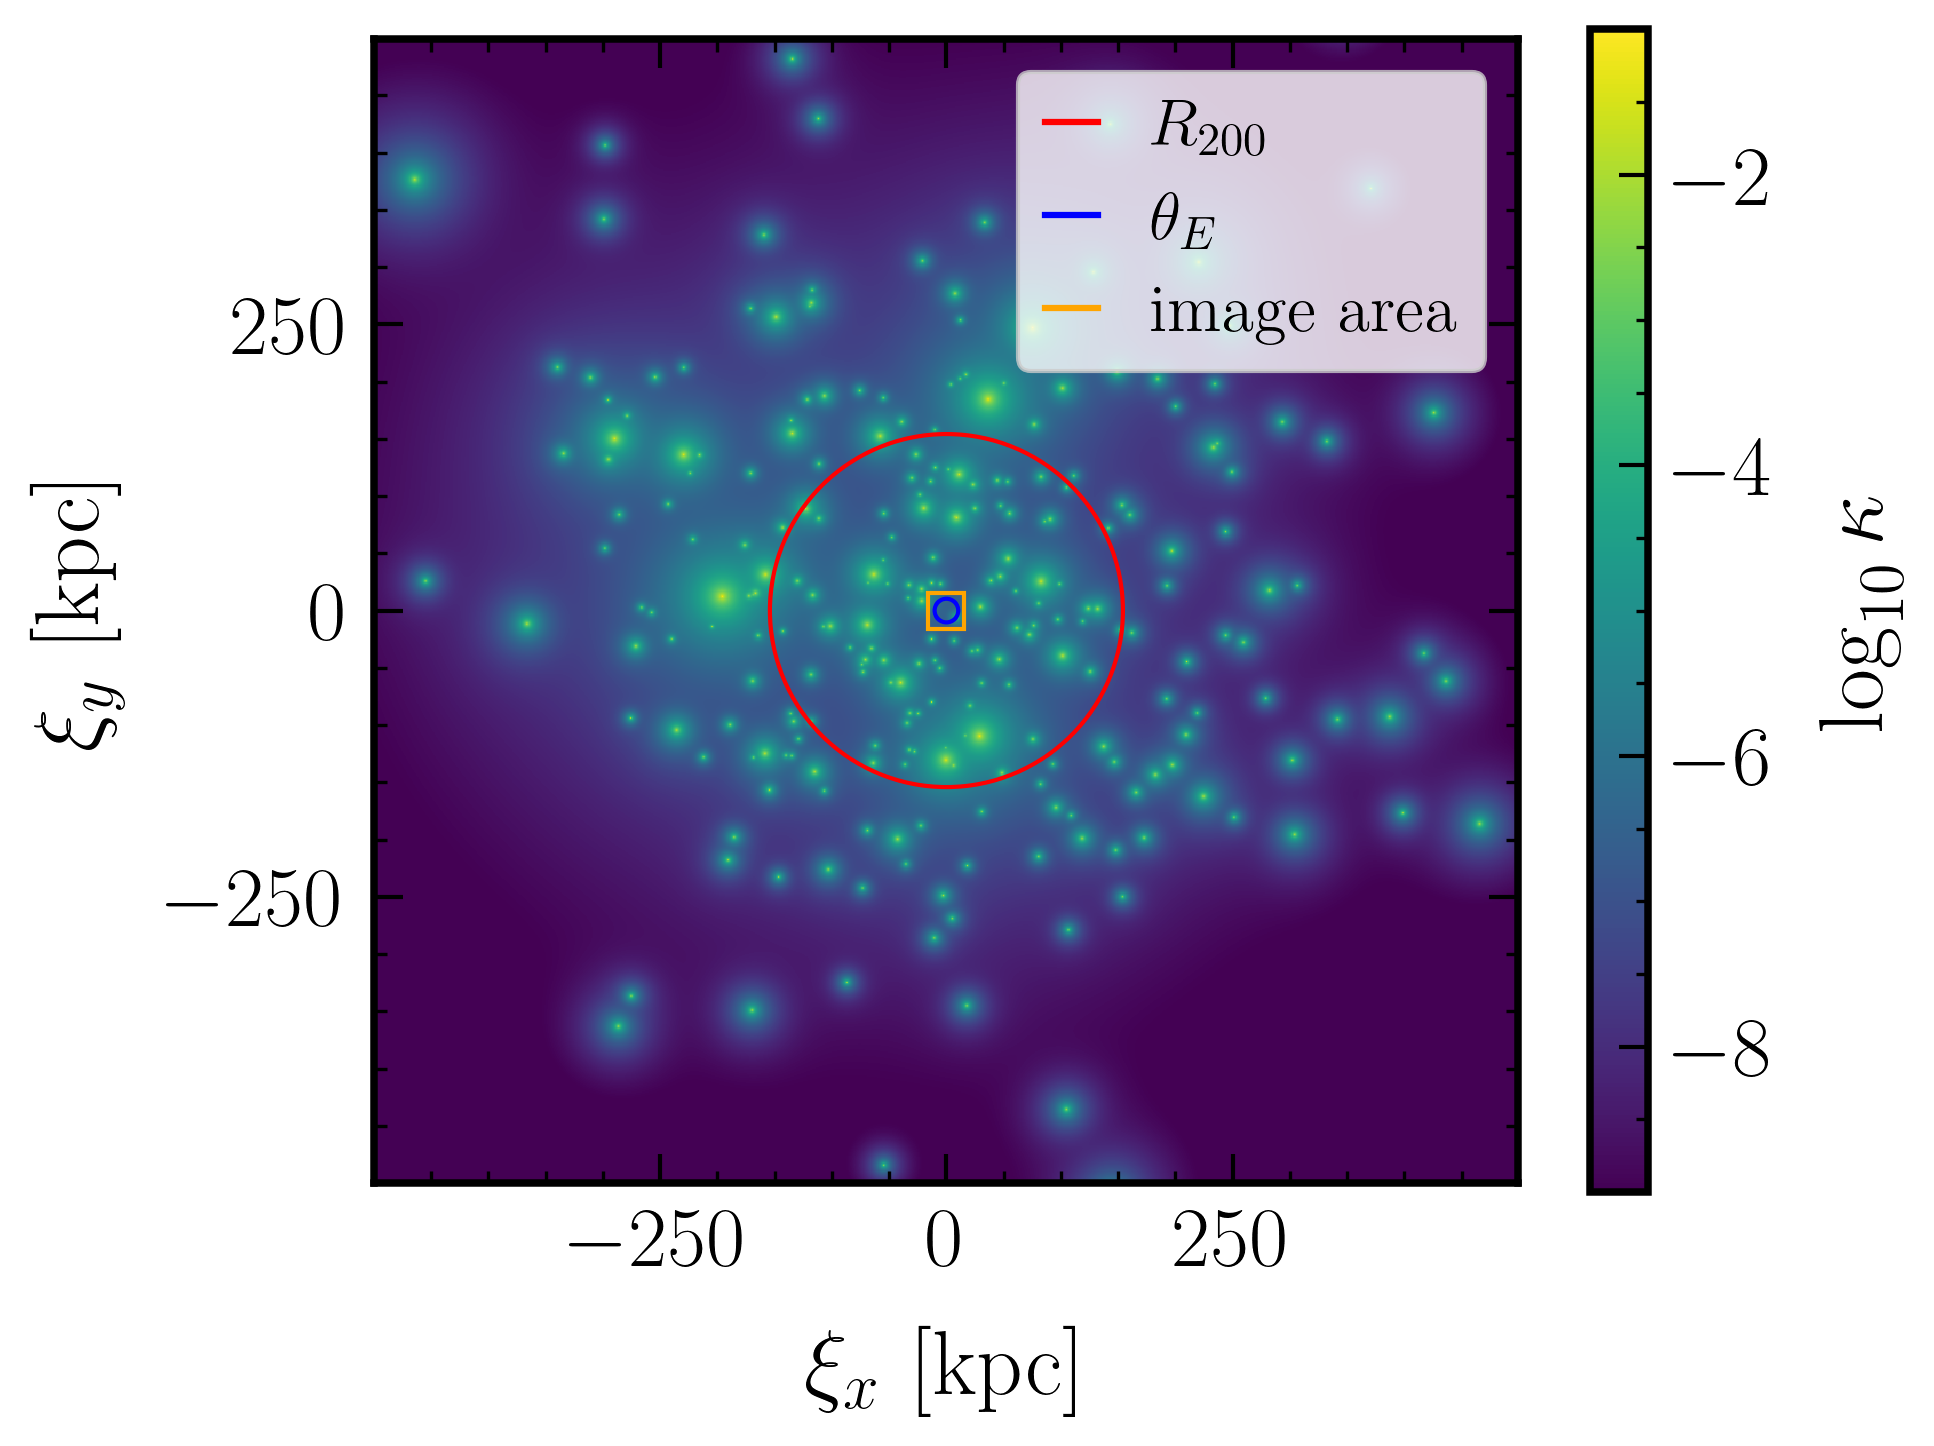
\includegraphics[width=\linewidth]{GL-sub-convergence.png}
	\end{subfigure}
	\hfill
	\begin{subfigure}[b]{0.46\linewidth}
	\centering
	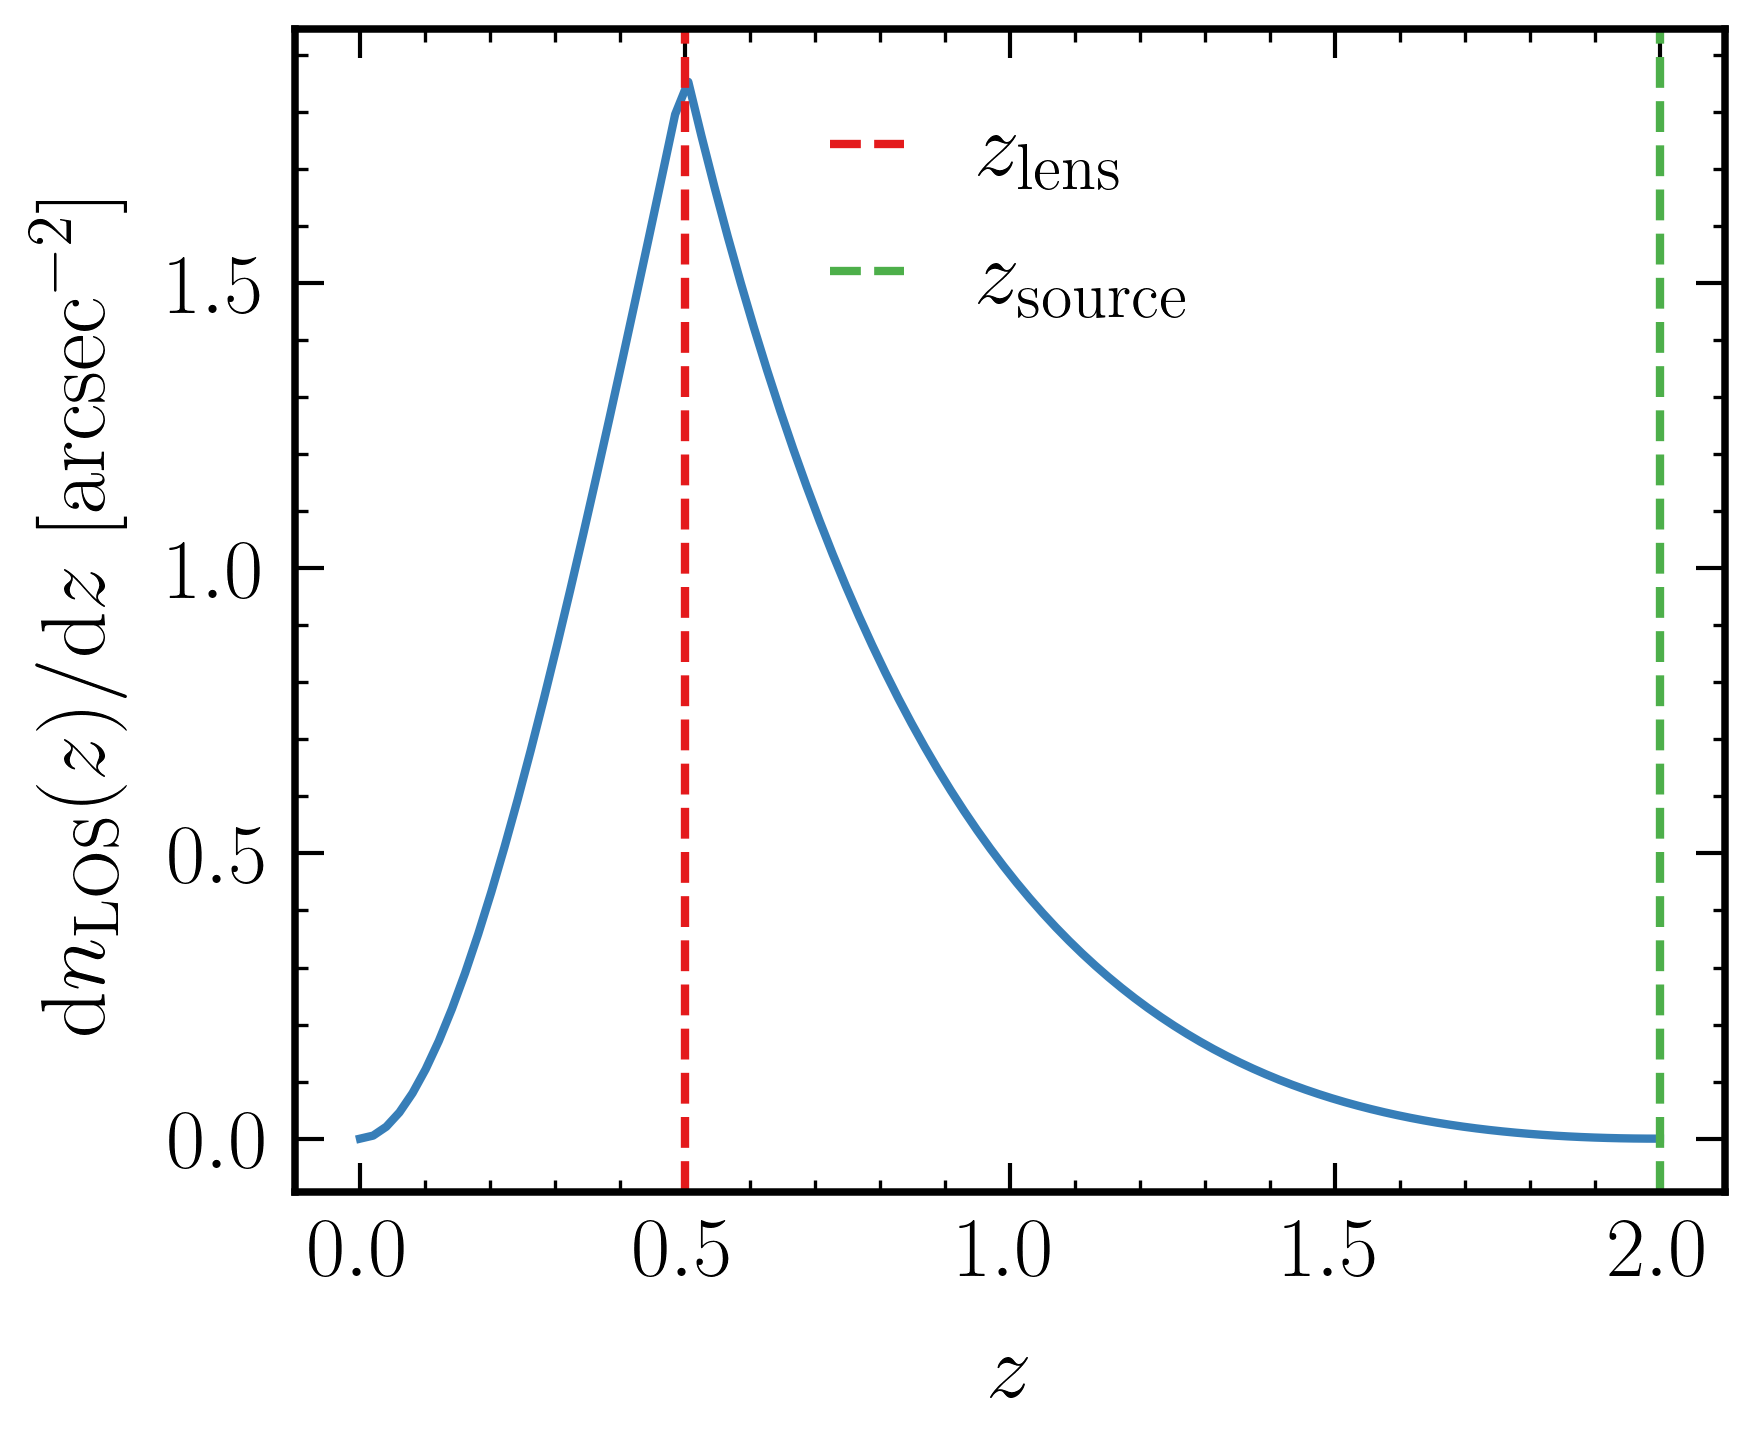
\includegraphics[width=\linewidth]{GL-los-z-dist.png}
	\end{subfigure} 
	\caption{\textit{Left panel:} Convergence map for a \gls*{cdm} subhalo population in the adopted mass range. The convergence map shows how the deflecting mass from all the subhalo lenses is distributed. The full map size is $1 \times 1\ \si{\Mpc}$. We mark in red the virial radius of the main lens halo, in blue its Einstein radius, and in orange the $5 \times 5\ \si{\arcsec}$ lensing image area. \textit{Right panel: }\gls*{los} halos distribution in redshift for our source and lens redshifts configuration, $z_\mathrm{lens}=0.5$ and $z_\mathrm{source}=2$.}
	\label{fig:sl-substructure}
\end{figure}

\Gls*{dm} substructures can be divided into two categories: subhalos that orbit around the main halo at the lens redshift, and \gls*{los} halos distributed between the source and the observer. \Gls*{los} halos are a more direct probe of free-streaming-induced small-scale structure suppression, because they are less affected by baryonic processes and environmental effects, such tidal stripping interactions with the main halo \cite{Despali:2017ksx}. For this reason and the fact that they are expected to be more abundant than subhalos in a lensing system \cite{Despali:2017ksx, He:2021rjd}, it is very important to model them as well, in order to correctly estimate the collective effects of all substructures on the lensing image. 

\subsubsection{Density profile}
To model the density profiles of small-scale \gls*{dm} halos we adopt the smoothly truncated universal 3D mass density profile from Ref.~\cite{Baltz:2007vq}:
\begin{equation}
    \rho_{\mathrm{tNFW}}(r)= \cfrac{\rho_s}{r/r_s (1+r/r_s)^2}  \cfrac{1}{1+(r/r_t)^2}.
\end{equation}
Here $r$ is the three-dimensional distance from the center of the halo, $\rho_s$ and $r_s$ are respectively the scale density and scale radius that specify a \gls*{nfw} profile \cite{Navarro:1996gj}, and $r_t\equiv\tau r_s$ is the tidal truncation radius that depends on the history of the subhalo. Typical values of the truncation scale $\tau$ range from $4-10$ for spherically symmetric lenses \cite{Gilman:2019nap, Cyr-Racine:2019aa}; we fix $\tau=6$ for simplicity. 
Compared to the standard \gls*{nfw} form, which has an infinite total mass, the truncated \gls*{nfw} contains an additional truncation term that makes the profile decay as $r^{-5}$ for large radii, resulting in a finite total mass given by:
\begin{equation}
    m_\tau=4\pi \rho_s r_s^3 \frac{\tau^2}{(\tau^2+1)^2}[(\tau^2-1)\ln\tau+\tau\pi-(\tau^2 +1)].
\end{equation}
With a fixed truncation scale, the truncated \gls*{nfw} profile is fully determined by the same parameters that determine the \gls*{nfw} profile: the virial mass $m_\mathrm{200, sub}$\footnote{We parameterize subhalos by what would be their mass up to the virial radius $r_{200}$ using the untruncated profile, with the same central density $\rho_s$ and scale radius $r_s$ as the truncated one. This is defined as the mass of the halo enclosed in a sphere where the untruncated halo's average density is 200 times the critical density.} and the concentration $c=r_{200}/r_s$ of the halo. The latter measures how concentrated the mass of a halo is and fixes the density normalization; in principle, it varies from one subhalo to the next and shows dependencies on mass and redshift of the main halo. Here, instead of adopting a concentration-mass relation, we fix $c_{200}=15$ , which is roughly the average value for perturbers in the mass range $10^7-10^{10}\si{\solmass}$ \cite[Figure 7]{Richings:2020auv}. We anticipate that accounting for scatter in the mass-concentration relation might actually improve our ability to measure subhalos’ parameters as higher concentrations lead to substantially stronger lensing signals \cite{Amorisco:2021iim}.
The equations for calculating the displacement field of a truncated \gls*{nfw} halo, given its mass and position, are fully elaborated in Appendix A of Ref.~\cite{Baltz:2007vq}.

To generate perturber populations, we must choose values for their density normalizations and scale radii. Since simulation studies typically measure the halo mass $m_\mathrm{200, sub}$ and the concentration $c$, it is more convenient to sample populations from distributions over these parameters. These variables can then be mapped to the parametrization above via
% The mass in this mapping actually corresponds to $m_{200}$ for an \emph{untruncated} NFW halo!
\begin{align}
    r_s &= \frac{1}{c} \left[ \frac{3 m_\mathrm{200, sub}}{4 \pi \, 200 \rho_\mathrm{cr}(z_\mathrm{lens})} \right]^{1/3} \, ,\\
    \rho_s &= \rho_\mathrm{cr}(z_\mathrm{lens}) \, \frac{1}{3} \frac{c^3}{\log(1+c) - c / (1 + c)} \, . 
\end{align}
For simplicity, we model \gls*{los} halos using exactly the same profile even though they typically have not undergone tidal stripping. 

The parameters of an individual subhalo which are not fixed are thus $\psubb \equiv (x_\mathrm{sub}, y_\mathrm{sub}, m_\mathrm{200, sub})$, where the second and third components are the projected position of the subhalo. In the case of \gls*{los} halos, the parameter set also includes the redshift $z_\mathrm{los}$. In the following sections, we will use arrows to denote vectors, \eg~$\vec{m}_\mathrm{200, sub}$ is an ordered set of masses, one for each simulated subhalo, and bold letters with an arrow to indicate arrays of vectors, \eg~ $\psub \equiv (\bm x_\mathrm{sub}, \bm y_\mathrm{sub}, \bm m_\mathrm{200, sub})$ is an ordered set of mass and positions in the lens plane, one for each simulated subhalo, and equivalently for \gls*{los} halos $\plos \equiv (\bm x_\mathrm{los}, \bm y_\mathrm{{los}}, \bm z_\mathrm{{los}}, \bm m_\mathrm{200, {los}})$. We collectively define the parameters of the full population of perturbers, subhalos and \gls*{los} halos, as $\pp$. In the next two subsections, we describe how we sample these parameters.

\subsubsection{Generating subhalos} \label{subsubsec:sl-model-sub}

We sample subhalo masses from the \gls*{cdm} mass function of Ref.~\cite{Giocoli:2009ie}:
\begin{equation} \label{eq:shmf}
    \frac{1}{m_\mathrm{200}}\frac{\dd n_\mathrm{sub}( m_\mathrm{200}, z)}{\dd\log m_\mathrm{200}} = A_M (1+z)^{1/2}m_{200}^{\alpha} \exp\left[-\beta\left(\frac{m_\mathrm{200}}{M}\right)^3 \right],
\end{equation}
where $M$ \footnote{
    The total mass of the lens galaxy is described by the Einstein radius of the system, a very well-constrained parameter in lensing inference analyses. For the purpose of describing subhalos, we need to be able to map the measured properties of the lens (the Einstein radius $\theta_\mathrm{E}$) onto the properties of the host halo (the mass $M$). For simplicity, we compute the mass of the host halo transforming the Einstein radius distance measure into a mass measure. We would like to point out a similar approach from \cite{Brehmer:2019jyt}, where they relate the central velocity dispersion of a singular isothermal ellipsoid lens mass distribution profile to the virial mass of the host halo.
}  is the mass of the main lensing halo and $m_\mathrm{200}$ the subhalo mass. The free parameters in this function were fit to hydrodynamical cosmological simulations that included baryons in Ref.~\cite{Despali:2016meh}. In particular, we use the fits to EAGLE, which give $\alpha = 0.85$ (given in the text) and $(A_M, \beta) = (2.4\times10^{-4}\, \si{\solmass}^{\alpha - 1}, 300)$ (extracted from their figures). The expected number of subhalos in a given mass interval for the lens halo system can be computed by integrating the mass function over that interval.

The spatial distribution of subhalos has been shown to follow an Einasto profile \cite{Springel:2008cc}. However, since the virial radius of a typical main lens halo is much larger than its Einstein radius, and hence, than the image plane, we approximate the distribution to be uniform in the lensing image area. Still, we derive the total number of expected subhalos within the image,  $\bar{n}_\mathrm{sub}$,  via the Einasto fit of Ref.~\cite{Despali:2016meh}. We find that on average $\bar{n}_\mathrm{sub}=4$ subhalos fall within the lensing image area in our adopted lensing configuration and mass range. %With the lens redshift we have chosen, over a $\SI{5}{\arcsecond} \times \SI{5}{\arcsecond}$ image and integrating over the mass range \SIrange{e7}{e8}{\solmass}, we find $\bar{n}_\mathrm{sub} = 3.1$. 
Thereafter we generate the subhalo population by sampling the number of subhalos from $\operatorname{Poisson}(\bar{n}_\mathrm{sub})$, drawing their masses from the subhalo mass function in Equation~\eqref{eq:shmf} and sampling their projected positions uniformly over the lens plane. Since the vast majority of subhalos fall outside the lens plane, we expect their lensing effect to be mostly degenerate with external shear, and thus do not simulate them. In the left panel of Figure~\ref{fig:sl-substructure} we show the convergence map for one realization of our subhalo population.

\subsubsection{Generating line-of-sight halos}

As described in Ref.~\cite{CaganSengul:2020nat}, we first compute the average number of \gls*{los} halos in the double-pyramid geometry connecting the observer, lens-plane and source. For each simulation we sample the number of \gls*{los} halos from $\operatorname{Poisson}(\bar{n}_\mathrm{los})$. We then sample their redshifts and projected positions uniformly over the double-pyramid region and draw their masses from the mass function in Ref.~\cite{Tinker:2008ff}, assuming an overdensity with respect to the critical density of the universe at the epoch of analysis of $\Delta=200$. 

More in details, we infer the number of detectable \gls*{los} halos by integrating their mass function in the mass range adopted for the analysis and within the double-cone volume
\begin{equation}
    \bar{n}_{\mathrm{los}}=\int_0^{z_\mathrm{src}}\int_{m_\mathrm{200,min}}^{m_\mathrm{200, max}} n_\mathrm{los}(m_\mathrm{200}, z)\dd{m_\mathrm{200}} \frac{\dd{V}}{\dd{z}}\dd z.
\end{equation}
On average we get $\bar{n}_{\mathrm{los}}=260$ \gls*{los} halos projected in our lens plane. Similarly to what we do with the subhalo population, when generating simulated images, we draw the number of LOS halos from $\operatorname{Poisson}(\bar{n}_\mathrm{los})$, we then sample their masses and redshift from the halo mass function and sample their projected positions uniformly over the lensing image area. As with subhalos, we ignore any \gls*{los} halos lying outside the double pyramid volume. In right panel of Figure~\ref{fig:sl-substructure} we show the distribution of \gls*{los} halos in redshift for our lens and source redshifts configuration.

To avoid expensive iterative ray-tracing through the lens planes of each \gls*{los} halo, we project them as effective subhalos into the lens plane, using the relations derived in Ref.~\cite{CaganSengul:2020nat} to rescale their scale radii and masses. Following Ref.~\cite{CaganSengul:2020nat}, \gls*{los} halos at comoving distance $\chi$ can be treated as subhalos on the main-lens plane with an effective projected mass density given by:
\begin{equation}
    \Sigma_{\chi, \mathrm{eff}}(D_L\vec{x};m_{200},r_s,\tau)= \Sigma(D_L\vec{x};m_{200,\mathrm{eff}},r_{s,\mathrm{eff}},\tau).
\end{equation}
The effective scale radius $r_{s,\mathrm{eff}}$ and mass $m_{200,\mathrm{eff}}$ are respectively
\begin{equation}
    r_{s,\mathrm{eff}}=\cfrac{D_L}{g(\chi)D_\chi}r_s,
\end{equation}
and
\begin{equation}
    m_{200,\mathrm{eff}}=f(\chi)\cfrac{\Sigma_{\mathrm{cr}, l}}{\Sigma_{\mathrm{cr}, \chi}}\left(\cfrac{D_l}{g(\chi)D_\chi}\right)^2m_{200}.
\end{equation}
The piecewise functions $f(\chi)$ and $g(\chi)$ are:
\begin{equation}
    f(\chi)= \begin{cases}
            1-\beta_{\chi l} & \chi \leq \chi_L \\
            1-\beta_{l\chi}  & \chi > \chi_L \\
            \end{cases},
\end{equation}
and
\begin{equation}
    g(\chi)= \begin{cases}
            1 & \chi \leq \chi_L \\
            1-\beta_{l\chi}  & \chi > \chi_L \\
            \end{cases},
\end{equation}
with $\beta_{ij}=\cfrac{D_{ij}D_s}{D_jD_{is}}$, where $D_i$ is the angular diameter distance from the observer to plane i, and $D_{ij}$ is the angular diameter distance from lens plane i to lens plane j, and $\chi_L$ is the comoving distance to the main-lens plane.
We have also introduced the critical surface density at plane i
\begin{equation}
    \Sigma_{\mathrm{cr}, i}\equiv \cfrac{c^2D_s}{4\pi G D_i D_{is}}.
\end{equation}

It should be noted that effective convergence methods, like the one we adopt \cite{CaganSengul:2020nat}, do not fully capture the subtleties and degeneracies of multi-plane lens analysis, by disregarding how, when a \gls*{dm} small-scale halo is not in the lens plane, the lens mass model can absorb its lensing signal \cite{Fleury:2021tke, Amorisco:2021iim, He:2021rjd}. The omission of this effect may lead to an overestimate of the \gls*{los} halos contribution and needs to be addressed before this technique can be safely used for the analysis of real data.

For \gls*{los} halos we adopt the same concentration and truncation scale values used for subhalos.


\subsection{Modeling free-streaming effects in WDM}
\label{subsec:free-streaming}

\begin{figure}
    \centering
    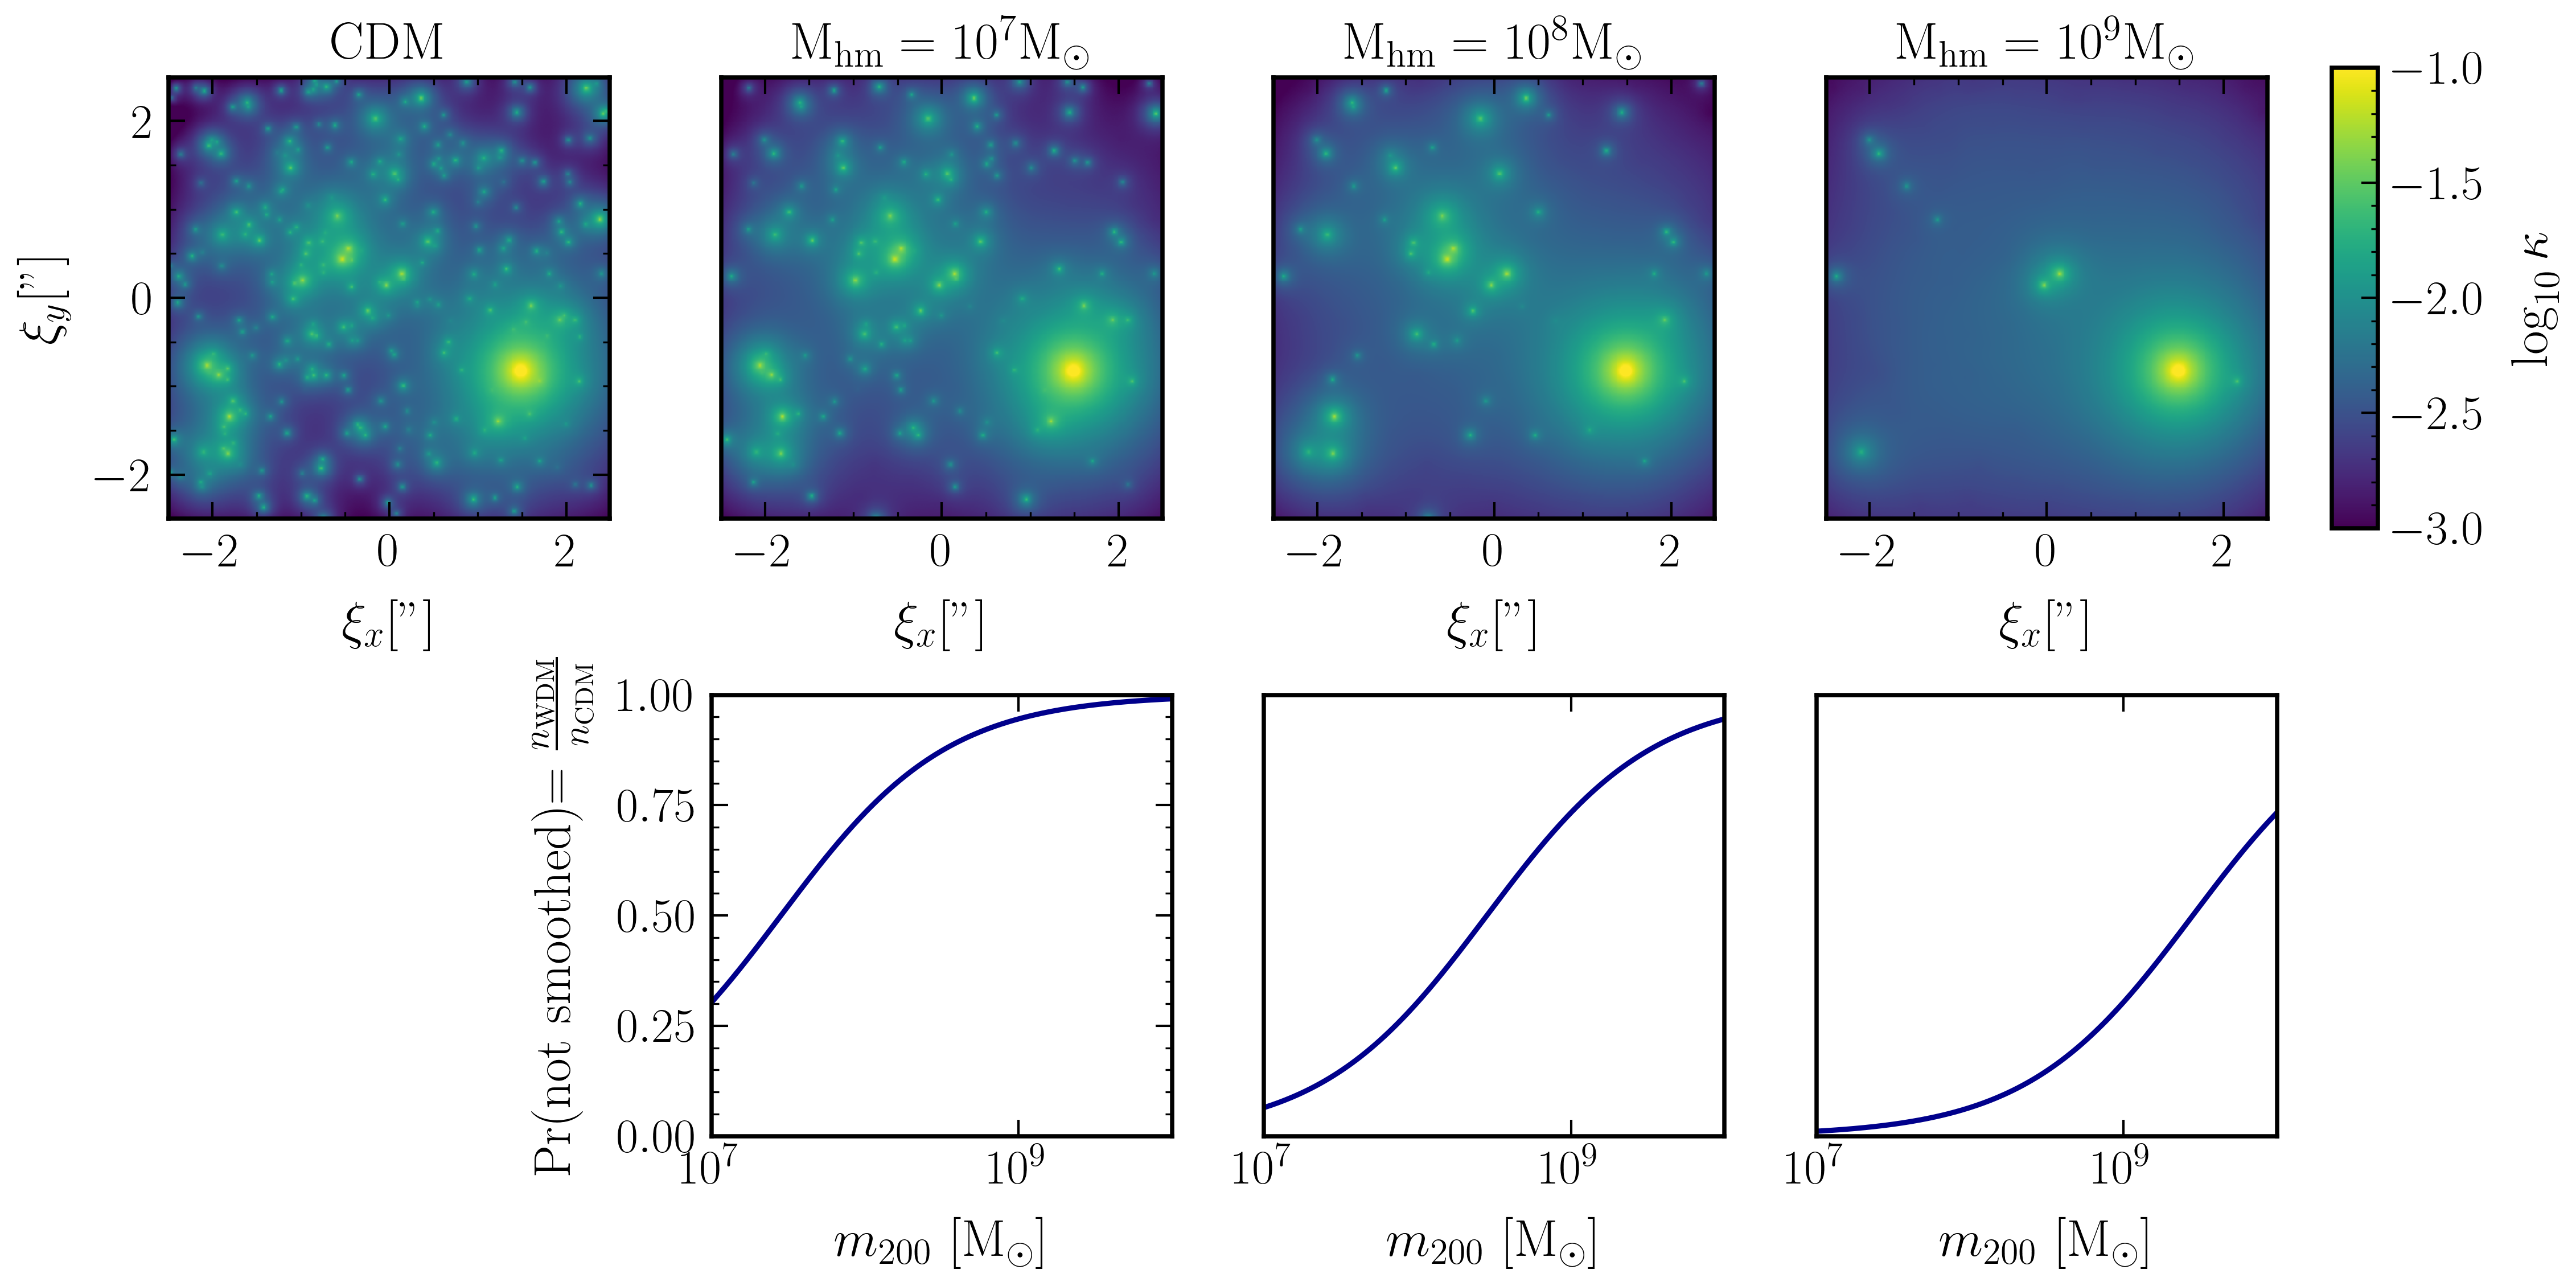
\includegraphics[width=\linewidth]{GL-smoothing.png}
    \caption{
    \textit{Top}: Convergence maps for a population of \gls*{los} halos with masses sampled from the \gls*{cdm} \gls*{hmf} in the adopted mass range (Table~\ref{tab:pop-model}) and projected in the lens plane following the prescription from Ref.~\cite{CaganSengul:2020nat}.
    In the second to fourth columns, we imitate the effect of \gls*{wdm} with different cutoff masses (as labeled in the titles) via our smoothing scheme. \textit{Bottom}: We show the probability with which \gls*{los} halos do not get smoothed, equal to the ratio between the \gls*{wdm} and the \gls*{cdm} \gls*{hmf} (see Equation~\eqref{eq:cutoff}). The smoothing is stochastic, so for each realization of the smoothing different halos are smoothed.
    }
    \label{fig:smoothing}
\end{figure}

In \gls*{wdm} models \gls*{dm} particles have non-negligible thermal velocities that allow them to free-stream out of density perturbations, effectively preventing small-scale structure formation. The free-streaming effects of \gls*{wdm} are well described in terms of the half-mode wavelength $\lambda_{\mathrm{hm}}$, which corresponds to the scale at which the \gls*{dm} transfer function falls to half the \gls*{cdm} transfer function. We can define the half-mode mass as the mass contained within a radius of the half-mode wavelength:
\begin{equation}
\mhm=\frac{4\pi\Omega_{\mathrm{M}}\rho_{\mathrm{crit}}}{3}\left(\frac{\lambda_{\mathrm{hm}}}{2}\right)^3,
\end{equation}
where $\Omega_{\mathrm{M}}$ is the matter density parameter and $\rho_{\mathrm{crit}}$ is the critical density of the universe.
Following \cite{Schneider:2011yu}, the half-mode wavelength,
\begin{equation}
    \lambda_{\mathrm{hm}}=2\pi\alpha_{\mathrm{hm}}\left(2^{\nu/5}-1\right)^{-1/(2\nu)},
\end{equation}    
is the scale below which the initial density perturbations are completely erased, with $\nu= 1.12$ and, assuming that all \gls*{dm} is warm,
\begin{equation}
\alpha_{\mathrm{hm}}=0.049\left(\frac{m_\mathrm{WDM}}{\si{\keV}}\right)^{-1.11}\left(\frac{\Omega_\mathrm{DM}}{0.025}\right)^{0.11}\left(\frac{h}{0.7}\right)^{1.22}h^{-1}\si{\Mpc}.
\end{equation}

We then have a one-to-one mapping between the mass of the \gls*{wdm} particle and the half-mode mass.
For strong lensing, the half-mode mass can be thought of as an effective cutoff mass below which the \gls*{dm} mass function is strongly suppressed. To model this suppression in the \gls*{wdm} mass function we adopt for both subhalos and \gls*{los} halos the functional form from Ref.~\cite{Lovell:2020bcy}:
\begin{equation}\label{eq:cutoff}
    \frac{n_{\mathrm{WDM}}}{n_{\mathrm{CDM}}}=\left(1+\left(\alpha\frac{\mhm}{m_{200}}\right)^\beta\right)^\gamma,
\end{equation}
with best fit parameters $\alpha=4.2$, $\beta=2.5$, and $\gamma=0.2$ for subhalos, $\alpha=2.3$, $\beta=0.8$, and $\gamma=1$ for central halos.

\subsubsection{Smoothing substructures}
\label{subsubsec:smoothing}

The observational signature of \gls*{wdm} is, thus, the absence of small-scale structures. However, in the current parameterization, this is accompanied by the removal of the corresponding mass enclosed in them, whereas in reality the mass will still be present but will be diffused throughout the smooth main halo. This effect is manifested in a correlation between the half-mode mass and the main-halo Einstein radius: suppressing more substructure leads to an increase in the inferred Einstein radius since the total mass of the system (within the image) is tightly constrained by the size of the observed ring (or arcs).

We introduce a prescription for dealing with this degeneracy, which well captures the physical reality of structure suppression due to free streaming. 
Halos that should be suppressed are not present because the \gls*{dm} particles that should make them up are freely streaming, and their mass is therefore more diluted throughout the main halo.
Therefore, rather than removing or adding substructures as a response to a changing cutoff, we still sample substructures from the \gls*{cdm} mass function, but we smooth the displacement field generated by halos that should be suppressed based on the aforementioned prescription by \cite{Lovell:2020bcy} to hide their lensing signature. In other words, each sampled small-scale halo has a probability equal to the ratio between the \gls*{wdm} and the \gls*{cdm} \gls*{hmf} (Equation~\eqref{eq:cutoff}) of not being smoothed. 

We then effect the smoothing by convolving the deflection field of each individual sub-/\gls*{los} halo with a radially-symmetric filter
\begin{equation}
f \propto 1 - \exp\left(-\left(\frac{r}{r_{\mathrm{smooth}}}\right)^{n_{\mathrm{smooth}}}\right).
\end{equation}
This filtering preserves the far-field lensing signature of the halo, which is only determined by its total mass.
By default, we choose the smoothing scale to be equal to the halo virial radius: $r_\mathrm{smooth}=r_{200}$, and the smoothing exponent $n_\mathrm{smooth}=2$.

In the top row of Figure~\ref{fig:smoothing} we visualize the convergence maps in the lens plane for the same realization of \gls*{los} halos drawn from \gls*{cdm} distributions (panel 1), and with different cutoff masses implemented with our smoothing scheme (panels 2-4). In the bottom row, we show how we decide to smooth the lensing signature of certain halos based on the ratio between the \gls*{wdm} and the \gls*{cdm} \gls*{hmf} (Equation~\eqref{eq:cutoff}). 


\subsection{Instrumental effects}

We generate mock data with comparable quality to \gls*{hst} observations. All images are $\SI{5}{\arcsecond} \times \SI{5}{\arcsecond}$ with $\SI{0.05}{\arcsecond}$ resolution ($100 \times 100$ pixels). In our simulations, we do not include a \gls*{psf} for simplicity, but this component cannot be disregarded in real data analysis. To account for the fact that each pixel in the image corresponds to a finite collecting region in the sky, we generate our images at a resolution eight times higher than the target resolution and downsample. In experiments we found that neglecting this effect can have a significant impact on inference results. Lastly, we add Gaussian and uncorrelated pixel noise to our observations such that the brightest pixels are approximately 30 times the noise level (after downsampling), representative of \gls*{hst} data.




\section{Methodology} \label{sec:sl-analysis}

Constraining the fundamental properties of \gls*{dm} by characterizing the population of \gls*{dm} halos in a strong lensing image is an extremely difficult problem since the signal we are interested in has a sub-percent level influence on images dominated by statistical noise. The problem is further complicated by the large differences between images of different lensing systems.

Our ultimate goal is to compute the marginal posterior $p(\mhm|\data)$ for a single parameter of interest $\mhm$, the half mode mass, given an observation $\data$, for which we have the generative model
\begin{equation}
\label{eq:model}
\begin{split}
    p(\data, &\psrc, \plens, \pp, \mhm) \\
    &= p(\data|\psrc, \plens, \pp, \mhm) p(\psrc)p(\pp|\plens, \mhm) p(\plens) p(\mhm)\; ,
\end{split}
\end{equation}
The first factor on the right-hand side is the simulator, while the other factors denote the priors on the various source, lens, and \gls*{dm} substructures parameters as listed in Table~\ref{tab:pop-model}. 

Therefore, in order to derive $p(\mhm|\data)$ we need to marginalize over all the nuisance parameters $\interest\equiv\{\plens, \psrc, \pp\}$:
\begin{equation}\label{eq:post}
     p(\mhm|\data) = 
     \frac{p(\data|\mhm)}{p(\data)} p(\mhm) =
     \frac{\int \dd{\nuisance} p(\nuisance) p(\data|\mhm, \nuisance)}{p(\data)} p(\mhm).
\end{equation}
This is a very high-dimensional and multi-modal integral, even for simple analytical lens and source models, due to the large population of interchangeable substructures. Therefore, it is intractable, which renders likelihood-based inference infeasible in this case.

Instead, we approximate $p(\mhm|\data)$ using \gls*{sbi} with the \gls*{tmnre} algorithm, presented in Section~\ref{sec:tmnre}.


Formally, inferring the marginal posterior for the substructure population parameter of interest would require marginalizing over all the source, lens, and substructure realizations compatible with all possible strong lensing images. However, sampling lens and source parameters from their priors would require a very large amount of training data and a more complex network architecture when using neural ratio estimation. This has been attempted only in Ref.~\cite{Brehmer:2019jyt} to infer the slope and normalization of the \gls*{hmf}. In order to reduce the complexity of the problem and fully exploit available information in the data with limited computational resources, we propose to target one image at a time, focusing simulations and the network training on a specific observation of interest. Thanks to \gls*{tmnre}, we implement this with a truncation scheme.

\gls*{tmnre} generates a sequence of likelihood-to-evidence ratio estimators on both nuisance and parameters of interest for a specific observation $\data$. In multiple inference rounds, the proposal distribution for nuisance parameters is updated and constrained, based on these ratio estimators, in order for the training data to match each round more closely the observation of interest $\data$ (this can be visually appreciated in Figure~\ref{fig:targeted_data}, which will be discussed in more details in Section~\ref{subsec:constrain}). 

The procedure for the truncation scheme is the following. In the first inference round, we generate training data sampling the nuisance parameters from the initial prior $p(\nuisance)$. Then, in each round, we constrain the proposal distribution $p_\Gamma(\nuisance)$ for the parameters we want to marginalize over to a region $\Gamma$ where the nuisance parameters are more likely to have generated $\data$ based on the ratio estimator trained in that round. In particular, we estimate the new region $\Gamma$ by very conservatively truncating the previous proposal distribution $p_\Gamma(\nuisance)$ in the region where the ratio estimator exceeds a predetermined threshold. We set the threshold hyperparameter to $\epsilon = 10^{-5}$, which, in case of a Gaussian posterior, corresponds to truncating at $\sim 4.78\ \sigma$ \cite{Miller:2022shs}. We obtain the final proposal distribution for our nuisance parameters when the region $\Gamma$ does not change significantly anymore between rounds. 


\medskip
In this work we target with \gls*{tmnre} a restricted set of the nuisance parameters $\nuisance$: namely, those of the analytic smooth lens and source models, $\plens$ and $\psrc$, while leaving halo parameters, $\pp$ unconstrained.

\medskip
To summarize, thanks to \gls*{tmnre}, the overall analysis strategy splits into the following steps:
\begin{enumerate}[leftmargin=1cm]
    \item[{1.}] Train an inference network to constrain the source and lens parameters, $\psrc$ and $\plens$, within ranges consistent with the observation. We then generate targeted training data based on this constrained model.
    \item[{2.}] Train an inference network to learn the marginal likelihood-to-evidence ratio for our parameter of interest, the half mode mass $\mhm$, on the targeted training data.
\end{enumerate}

Similarly to the reasoning behind the \gls*{abc} rejection algorithm, which discards sampled parameters values if the generated data is too different from the observed data, we justify this approach by noting that parameters that do not produce observations similar to $\data$ will not contribute to the integral in Equation~\eqref{eq:post}. Restricting the input parameters in this way immensely reduces the variability of simulated data, which allows us to use simpler network architectures and fewer training examples in the next step. As a result, the inference is now \emph{targeted} to the specific observation at hand rather than amortized over all the possible lens/source combinations from the full prior. We would like to point out that the inference is still locally amortized in the constrained proposal distribution region, and this enables empirical test of the inference result (see Section~\ref{subsec:test}).



\section{Experiment} 
\label{sec:sl-results}

%A population of low-mass halos can collectively cause perturbations to images that can be detected statistically in order to constrain the \gls*{hmf}. 
%In reality, constraining collective substructure properties from gravitational lensing images is an extremely difficult problem. 
%From measuring the distributions of perturbers' masses and other parameters, it is possible to infer population-level properties like the (sub)halo mass function parameters, which are dictated by the fundamental properties of dark matter.

In this section, we show our results for hierarchical population parameters inference. First, we describe the simulated data in Section~\ref{subsec:pop-data} and the inference network architecture in Section~\ref{subsec:pop-nn}. We then show how we constrain the lens and source parameters in Section~\ref{subsec:constrain}. Next, we show our results for the \gls*{hmf} cutoff mass and describe how we can combine the information from different strong lensing images in Section~\ref{subsec:dm}. In the same section, we show our results on the \gls*{dm} mass inference. Finally, we directly assess the statistical behavior of the trained neural networks in Section~\ref{subsec:test}.

\subsection{Mock data generation} 
\label{subsec:pop-data}

\begin{figure}
    \centering
    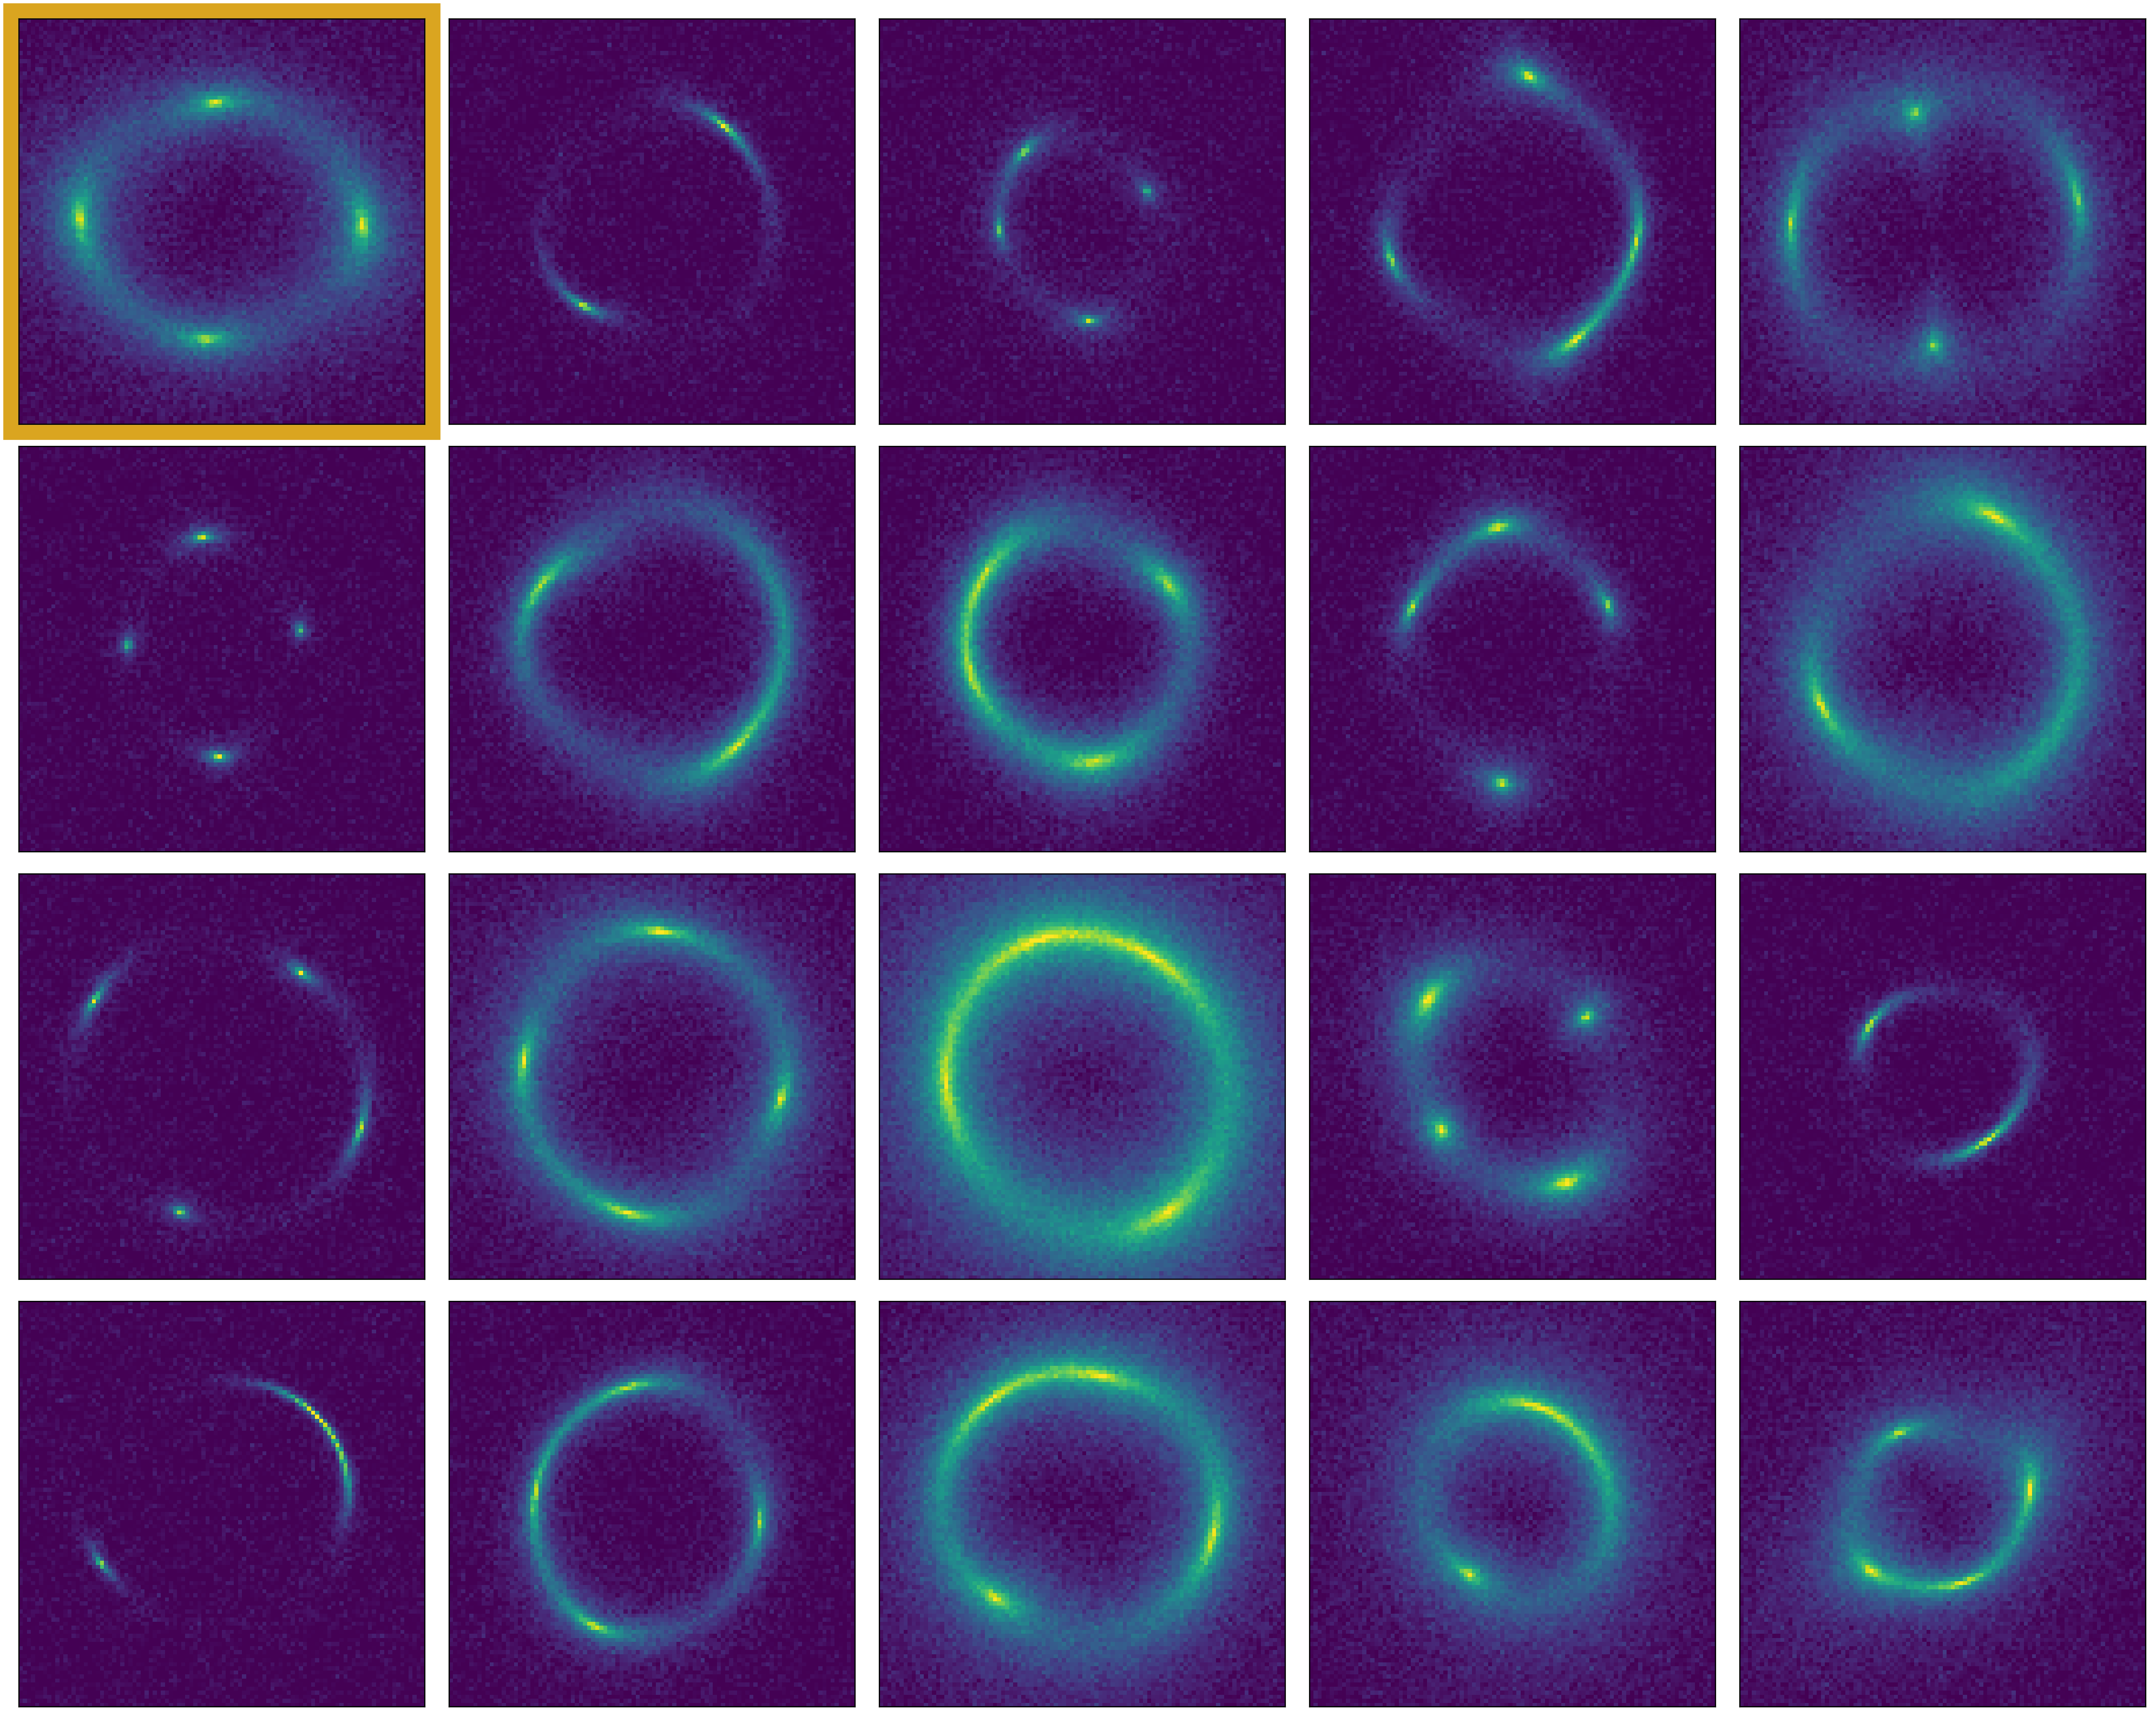
\includegraphics[width=\linewidth]{GL-mock.png}
    \caption{We present a gallery of twenty mock strong-lensing images we use as target observations. These mock observations have been generated with arbitrary lens and source parameters drawn from the initial prior in Table~\ref{tab:pop-model}. Their peak \gls*{snr} is $\num{\sim 30}$, representative of \gls*{hst} data. We analyze these images by first constraining their lens and source parameters proposal distribution in Section~\ref{subsec:constrain}. Then, we combine them in order to infer the cutoff mass scale in Section~\ref{subsec:dm}. For the first one (upper left corner, framed in orange) of these images we show our results of the first part of the pipeline (Section~\ref{subsec:constrain}) in Figure~\ref{fig:bounds}, Figure~\ref{fig:targeted_data}, and Figure~\ref{fig:lens_source_post}.
}
\label{fig:mock}
\end{figure}

For this inference task we use our lensing simulator at its full capacity, by including lens, source, substructures and different \gls*{dm} models that depend on the half-mode-mass \mhm:
\begin{equation}
    p(\data\mid\psrc, \plens,\pp, \mhm)
    = \mathcal{N}(\data\mid\mathrm{obs}(\psrc, \plens, \pp, \mhm), \sigma^2).
\end{equation}

In Figure~\ref{fig:mock} we show a gallery of twenty mock strong-lensing images we use as target observations. These mock observations have been generated with arbitrary lens and source parameters drawn from the initial prior in Table~\ref{tab:pop-model}. Their peak \gls*{snr} is $\num{\sim 30}$, representative of \gls*{hst} data.


\subsection{Neural network}
\label{subsec:pop-nn}

For all tasks we use the same general ratio estimator architecture, as seen in Section~\ref{subsec:tmnre-nn}. It consists of an initial compression network $C_\Phi(\data)$ that maps the $100 \times 100$ pixel images into a feature vector. This feature vector is concatenated to the parameters we want to infer (\eg~to $\psrc$ and $\plens$ for tasks where they are constrained, and $\mhm$). The vector is then passed to a binary classification network $d_\Phi(\data, \interest)$ which outputs an estimate of the 1D marginal likelihood-to-evidence ratios for the parameter of interest (with separate \gls*{mlp}s used to estimate the 1D ratios for $\psrc$ and $\plens$). For the embedding network, in both steps of the pipeline, we adopt a simple \gls*{cnn}. In Figure~\ref{fig:cnn} we show the \gls*{cnn} architecture used to constrain lens and source parameters. The one used to estimate the cutoff mass has a similar structure.

While we did not perform a full hyperparameter exploration, we found the batchnorm layers to be crucial for stable training of the \gls*{cnn} used for the macromodel ratio estimator.

\begin{figure}
	\centering
	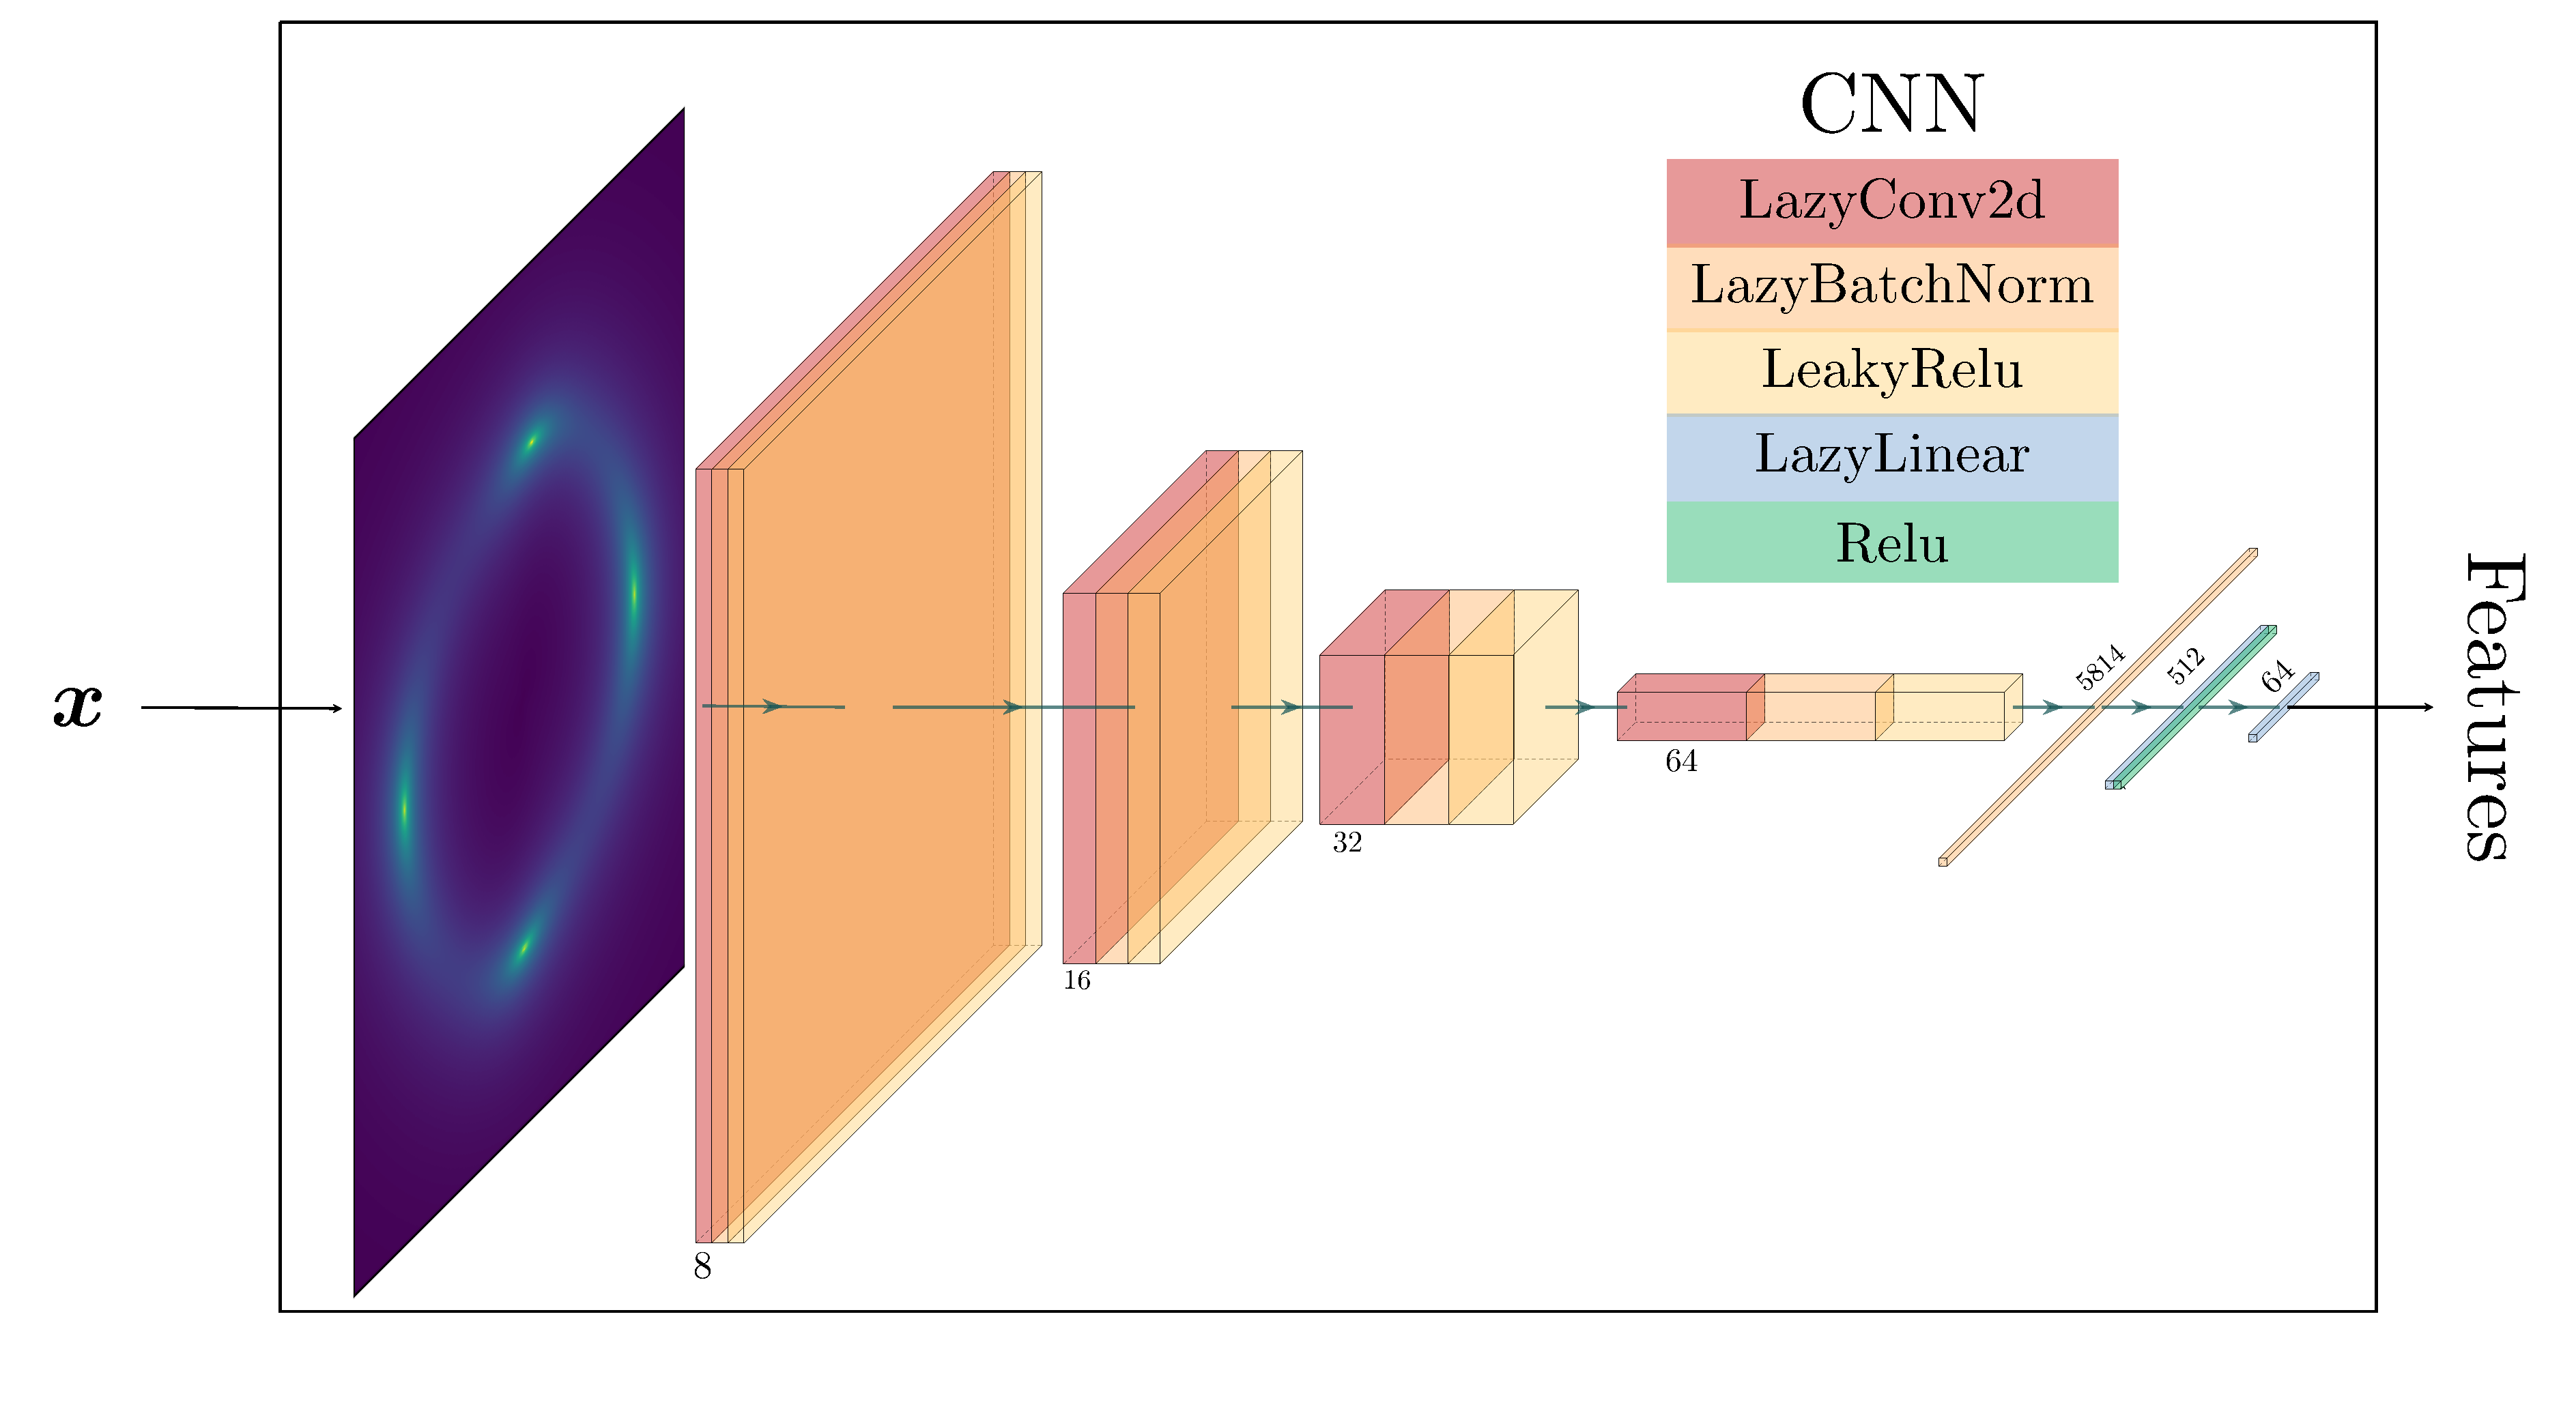
\includegraphics[width=\linewidth]{GL-cnn.pdf}
	\caption{Illustration of the embedding \gls*{cnn} architecture used in the first part of the pipeline to constrain lens and source parameters. The observation $\data$ gets compressed into features: estimates of the best possible data summary statistic, by the \gls*{cnn}. In describing the \gls*{cnn} layers we follow \texttt{PyTorch} \cite{pytorch} convention. To create the illustration we have used \cite{PlotNeuralNet}.}
\label{fig:cnn}
\end{figure}


\subsection{Constraining lens and source parameters}
\label{subsec:constrain}

\begin{figure*}
	\centering
	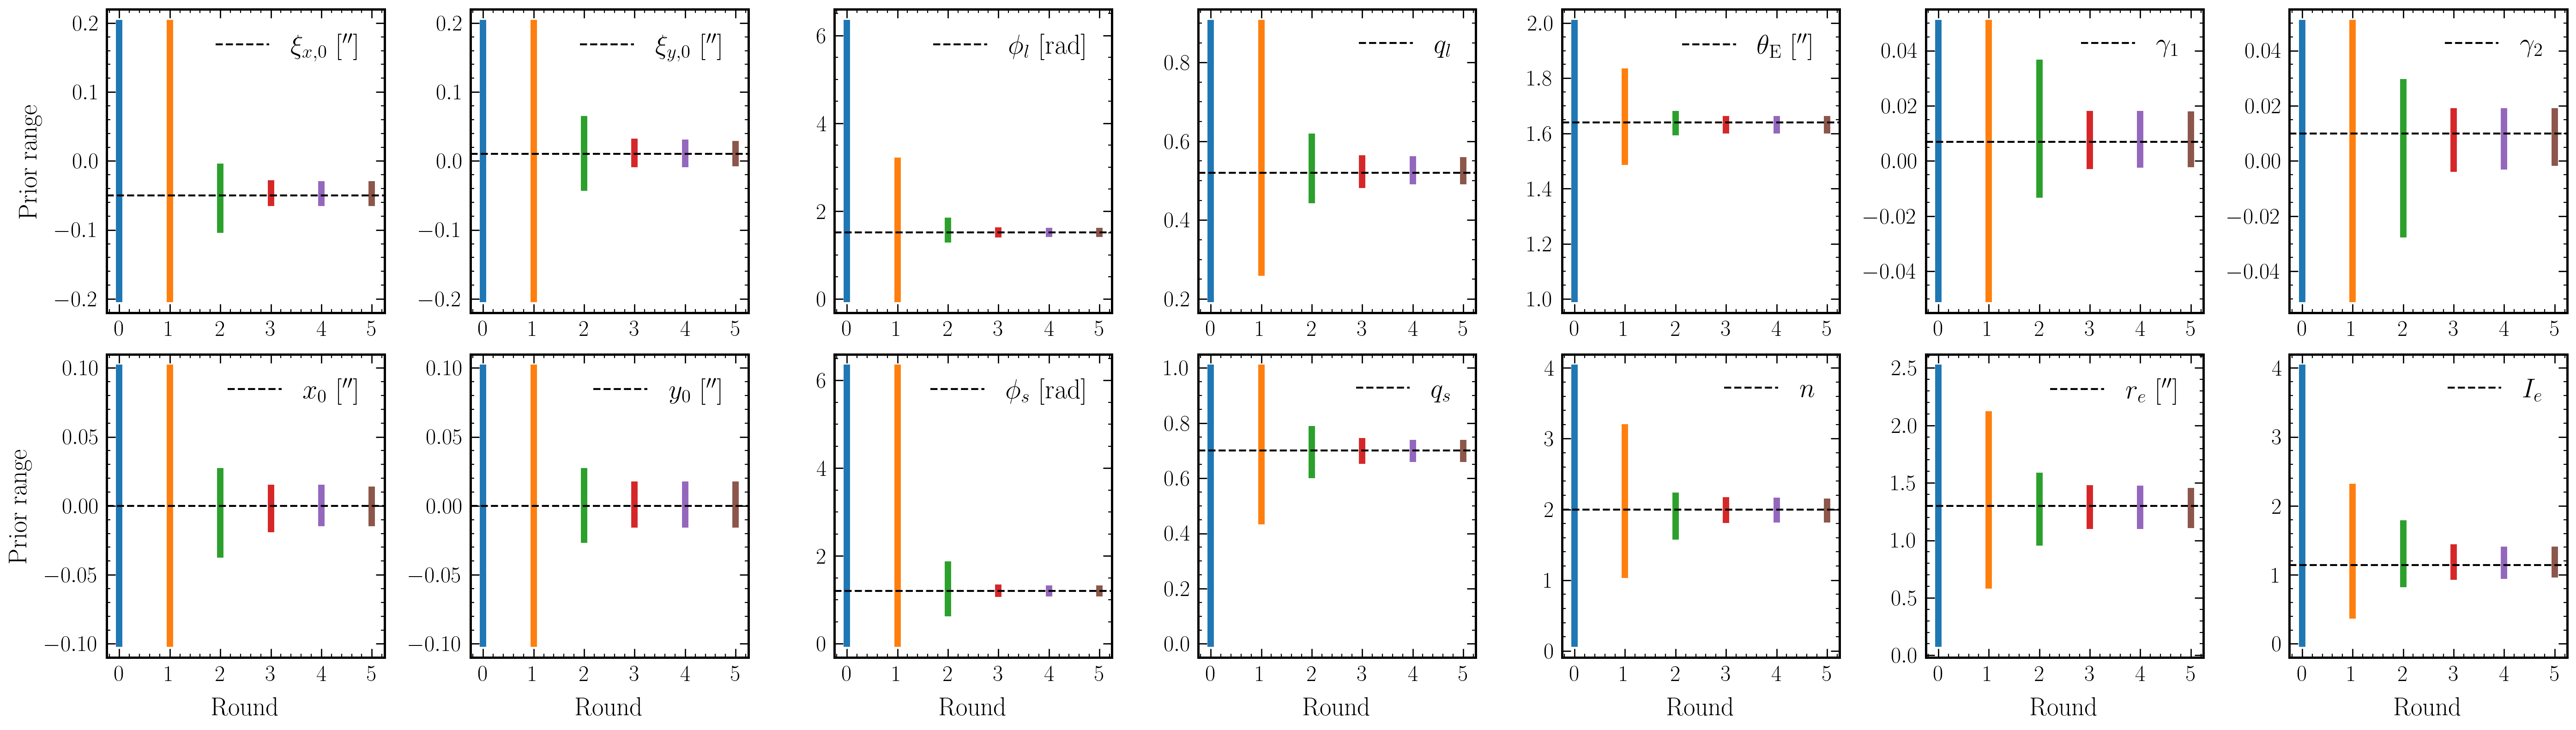
\includegraphics[width=\linewidth]{GL-bounds.png}
	\caption{Constrained proposal distribution. Visualization of the sequential truncation of the lens and source proposal distributions over the six rounds of training. The particular target is the first mock image (framed in orange in Figure~\ref{fig:mock}), whose parameters are depicted as black dashed horizontal lines.}
\label{fig:bounds}
\end{figure*}

\begin{figure}
	\centering
	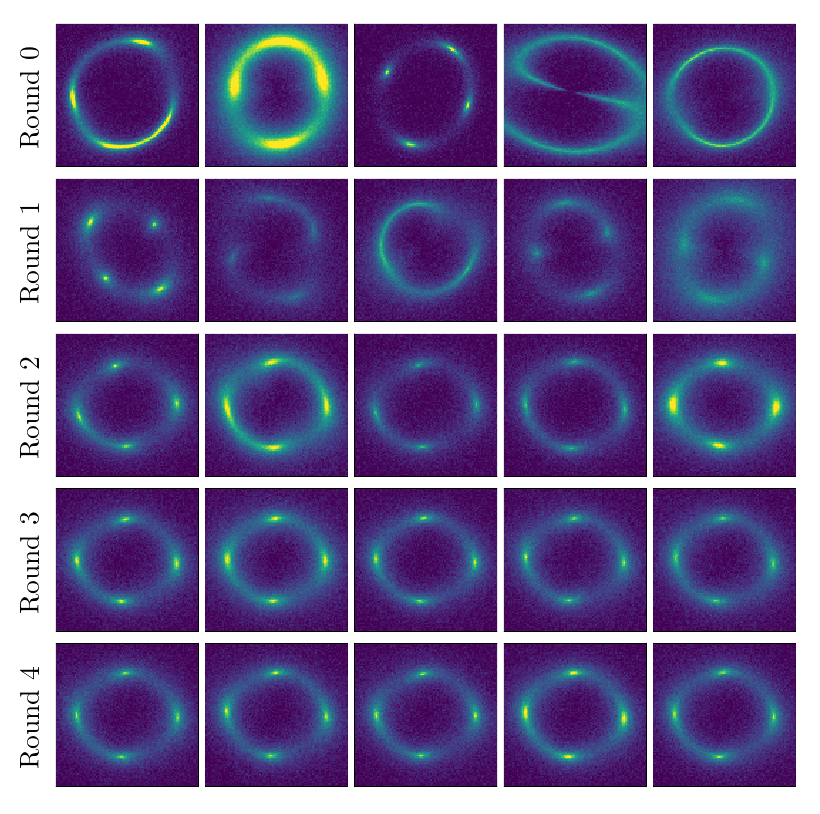
\includegraphics[width=\linewidth]{GL-targeted_data.png}
	\caption{Training data targeting the first mock observation (framed in orange in Figure~\ref{fig:mock}). In each row, we show five examples of training data for the first five rounds. In the first round, we sample our data from the initial prior shown in Table~\ref{tab:pop-model}. For the following rounds, the lens and source parameters are sampled from the constrained proposal distributions, obtained by evaluating the network trained with the previous round dataset on our target observation (see Section~\ref{subsec:constrain}). It is evident that with each round the training data more closely resembles the target image $\data_0$.}
\label{fig:targeted_data}
\end{figure}

\begin{figure*}
	\centering
	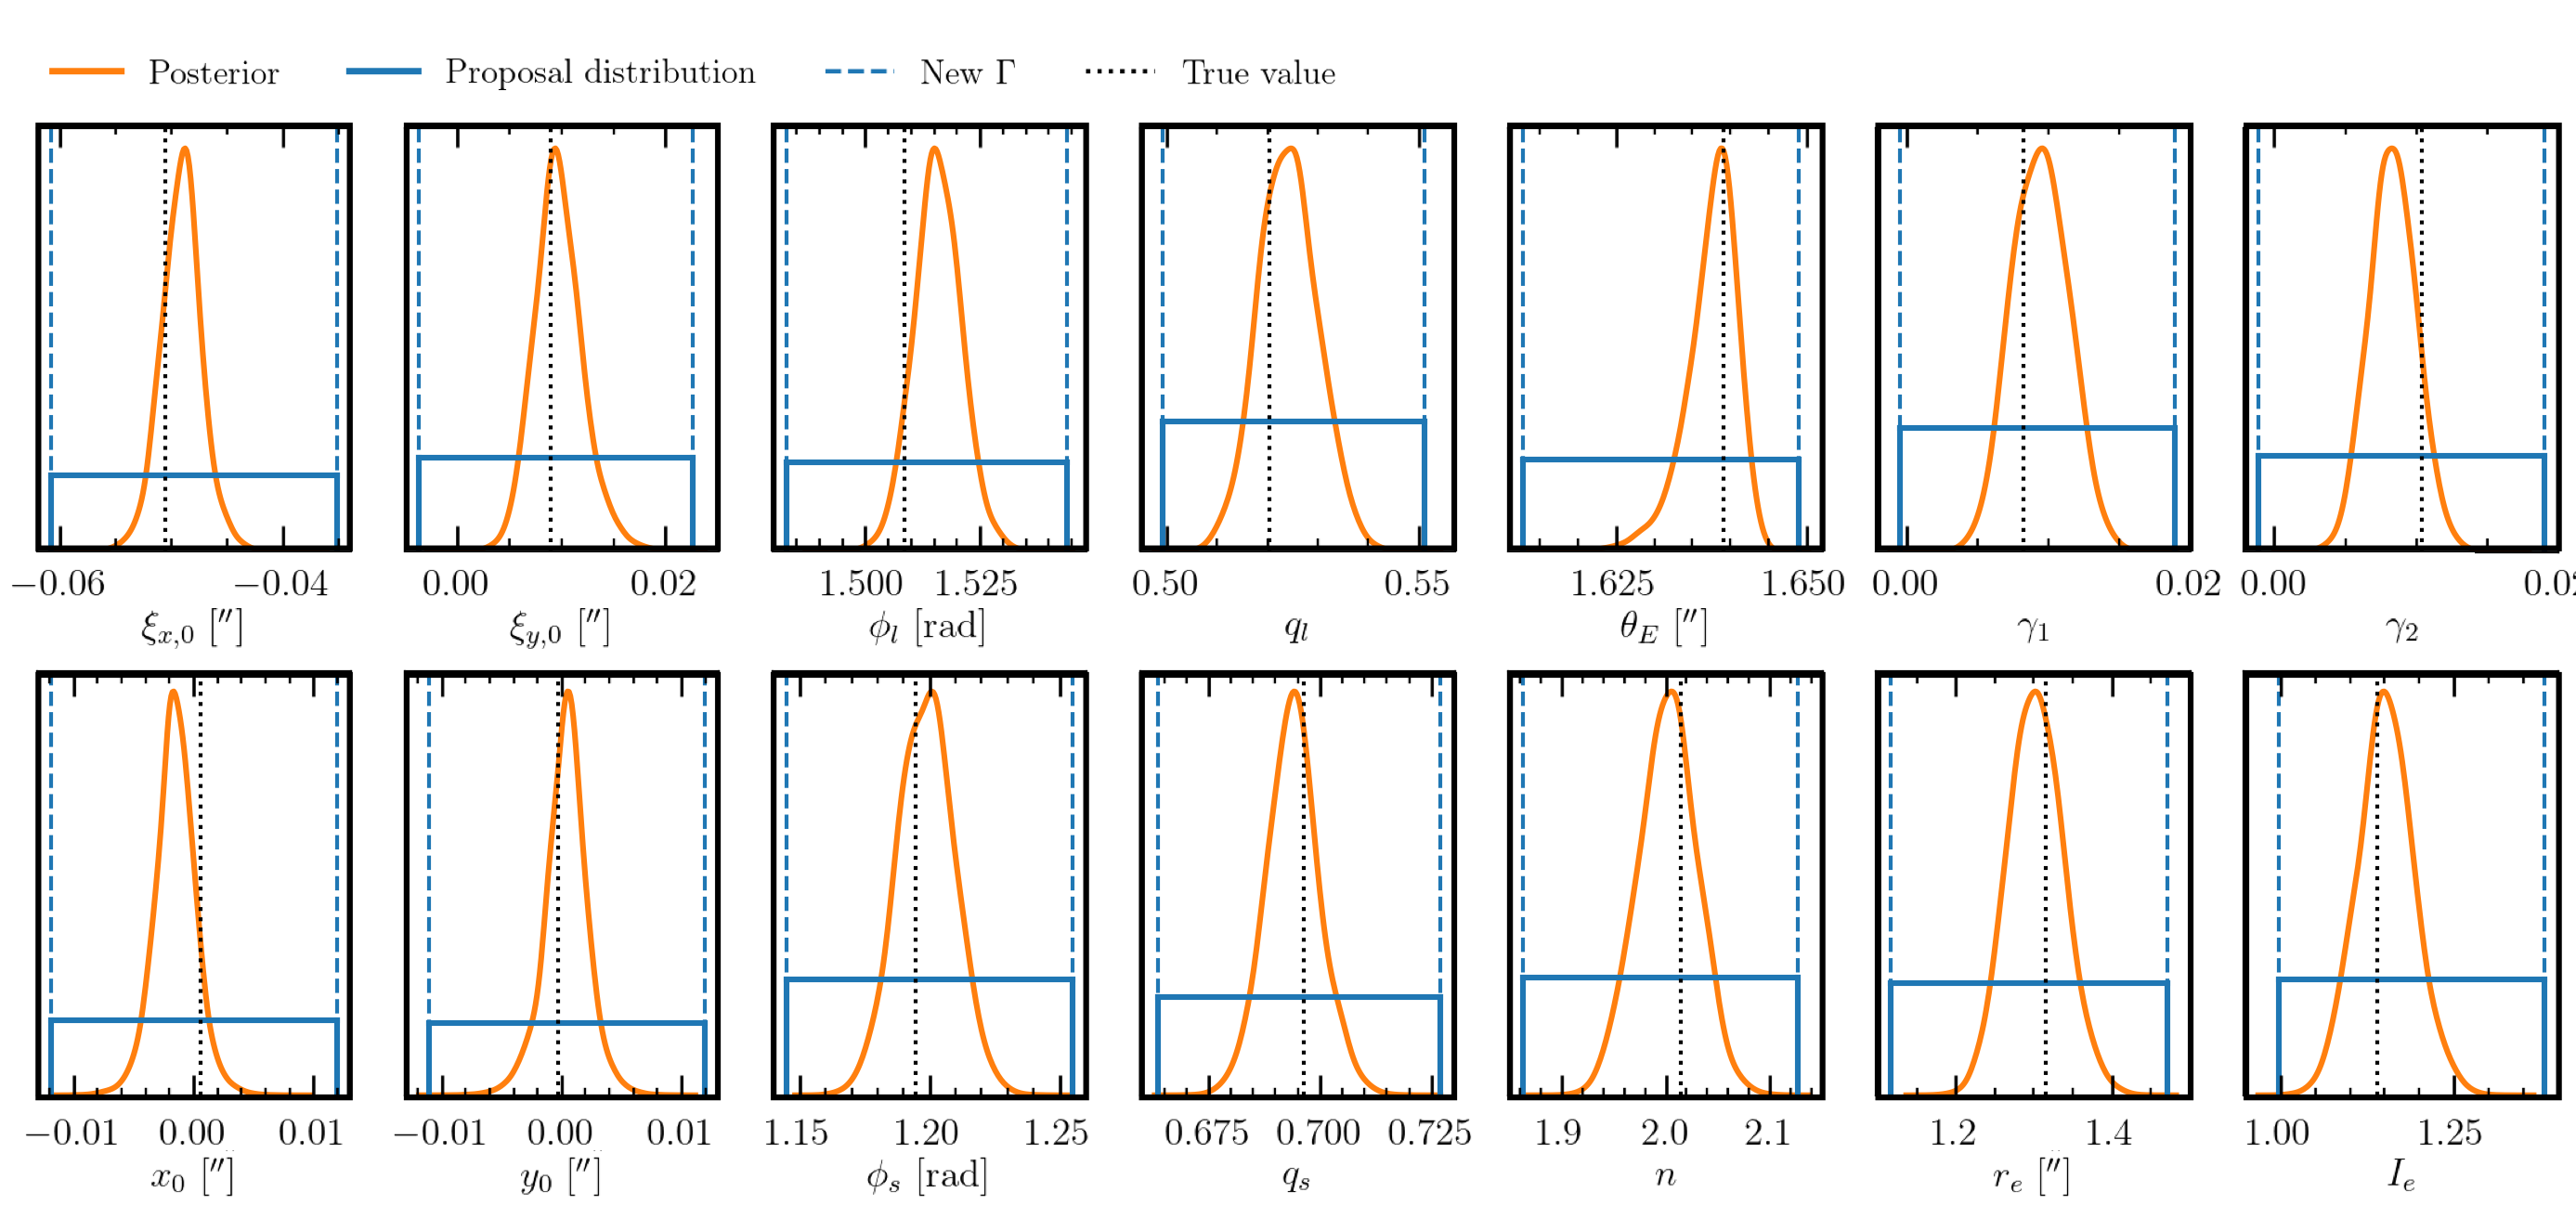
\includegraphics[width=\linewidth]{GL-lens_source_post.png}
	\caption{Lens and source parameters posteriors. In solid blue we show the last round of constrained proposal distributions for the first (upper left corner, framed in orange) target image in Figure~\ref{fig:mock}. The dotted black lines correspond to the true lens and source parameters values with which we have generated the target image. In orange, we show the estimated posteriors for lens and source parameters in the last training round. Based on the predetermined threshold, the new bounding limits $\Gamma$ (dashed blue) do not change significantly from the previous constrained proposal distribution region, so it is not possible to constrain the proposal distribution more and we stop the truncation procedure.}
\label{fig:lens_source_post}
\end{figure*}

We constrain lens and source parameters regions with \gls*{tmnre} (Section~\ref{sec:tmnre}) with multiple sampling and training rounds.

In total, we perform six sampling and training rounds. In each round, we simulate $10^5$ observations, of which $90\%$ are used as the training dataset, and the remaining $10\%$ as the validation dataset. Evaluations of the network on the mock target image are used to truncate the training data proposal distribution after each round, so that the region for lens and source parameters is targeted. The first training round is performed on the dataset generated from the initial source and lens parameters priors, shown in Table~\ref{tab:pop-model}. In Figure~\ref{fig:bounds} we show the initial prior and the following constrained proposal distributions. It can be seen that after the first round just a few of the parameters proposal distributions get truncated, \eg~the Einstein radius. By having truncated these initial parameters, in the following rounds the other parameters can be better learned by the network and so constrained. In Figure~\ref{fig:targeted_data}, we show samples from the first five training datasets, which demonstrate that the constrained regions are indeed the ones that are likely to produce data similar to the targeted image $\data$. After the sixth round of training, it is not possible anymore to truncate the proposal distribution region based on the predetermined threshold, as seen in Figure~\ref{fig:lens_source_post}. The truncation scheme has then efficiently identified the constrained region for lens and source parameters consistent with the targeted observation. Using the last constrained dataset, it is then easier in the second step of the pipeline to train a marginal neural ratio estimator to perform the final inference on the cutoff mass.

We would like to stress that these constrained proposal distributions correctly account for lens and source parameters uncertainties. In all our simulated data, the substructure parameters $\pp$ are randomly sampled from their prior, in order to account for the presence of substructure. This has the desirable outcome of approximately accounting for the average effect that an additional mass component has on the main lens parameters (\eg\ inferring an unbiased Einstein radius) and contributes to the source and lens uncertainties.

\subsection{Dark matter inference}
\label{subsec:dm}

For the second step of the pipeline, we train an inference network to learn the cutoff mass on the last constrained dataset. 

From initial tests, we have found that features from a single image are very hard to learn for the classifier, resulting in a very noisy ratio estimator.
In order to reduce the estimator uncertainty, we then train the cutoff mass classifier on a dataset $X^N=\{\data_1, ..., \data_N\}$ of $N$ different observations. For each observation, first, we constrain its lens and source parameters as explained in Section~\ref{subsec:constrain}. Then, we train the cutoff classifier on the concatenation of the features coming from their embedding networks, effectively learning $r(\mhm; X^N)$. 
Note that the images in one dataset are sampled with the same cutoff mass $\mhm$, but different lens, source, and substructures realizations. In fact, our final goal is to apply the full pipeline to real data, which will all have different source, lens, and substructures configurations, but will have encoded the same \gls*{dm} properties. 

\begin{figure*}
	\centering
	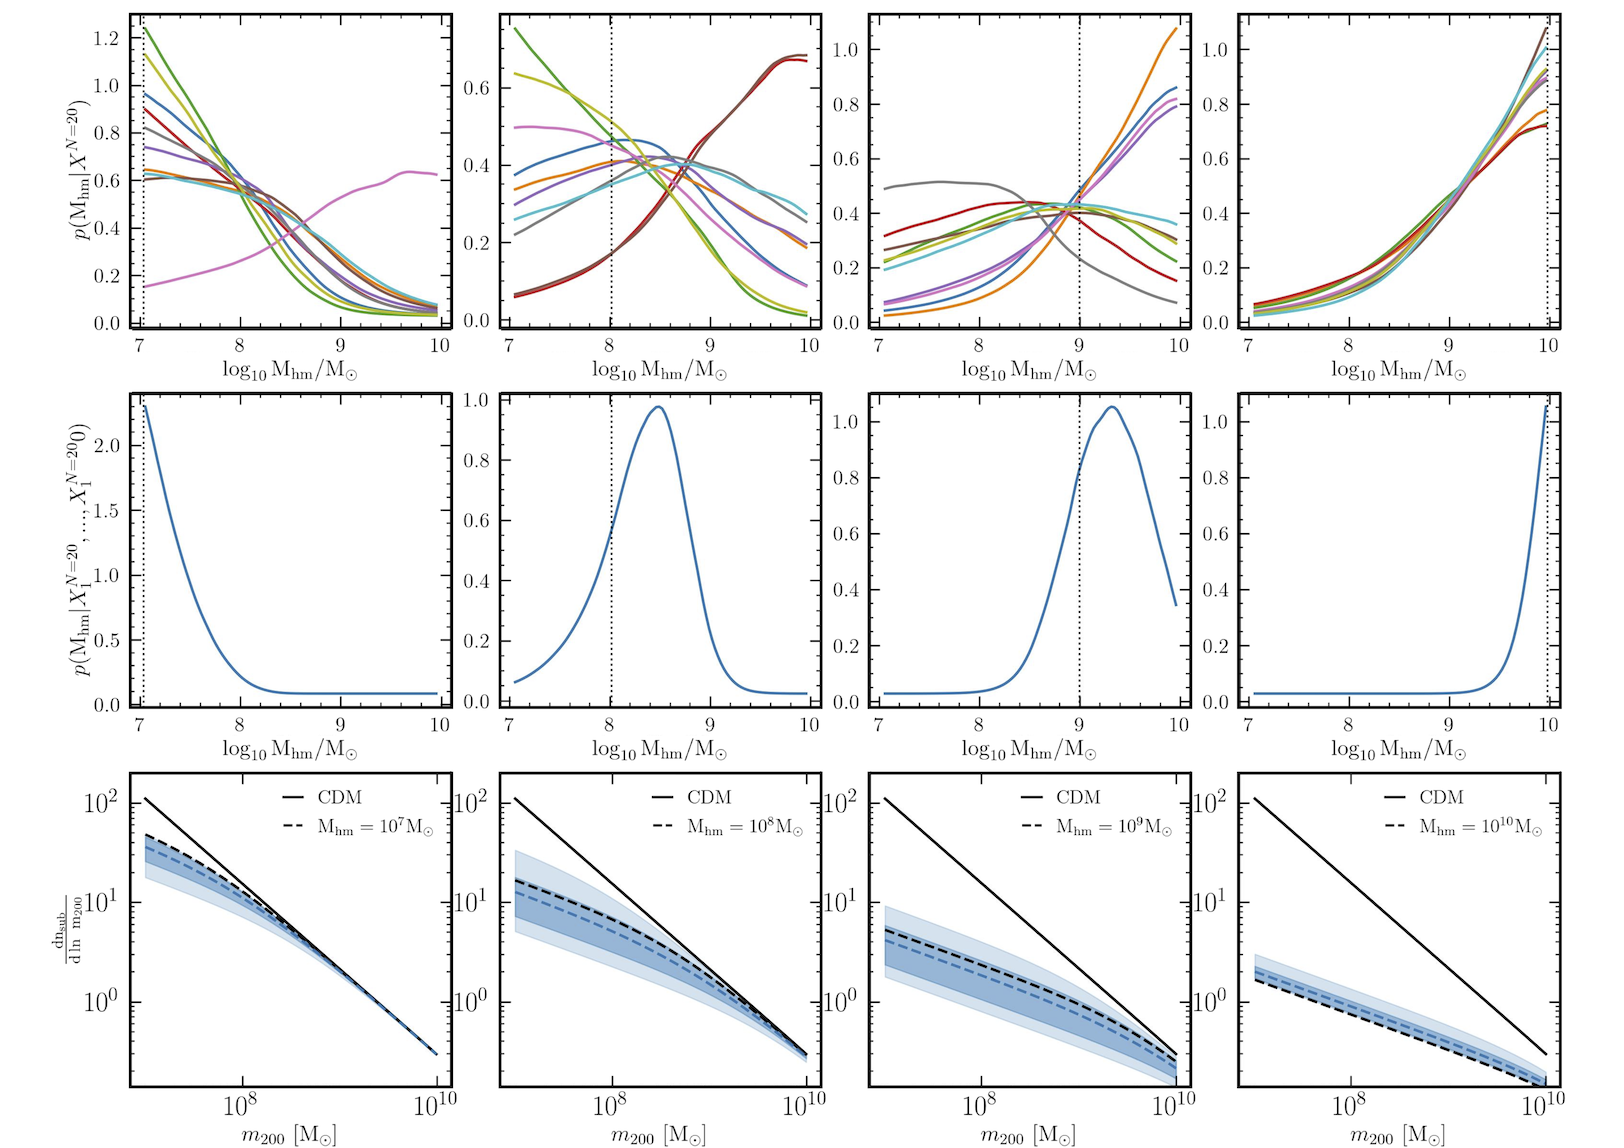
\includegraphics[width=\linewidth]{GL-mhm_results.png}
	\caption{\textit{Top:} Approximate posteriors for the half-mode mass derived from 10 different sets of 20 images. The dotted black line represents the true value of the half mode mass with which we have generated the images ($10^7, 10^8, 	10^9,  10^{10} \ \si{\solmass}$). \textit{Middle:} We show the approximate posterior resulting from the combination of the $M=10$ different posteriors shown in the first column, as explained in the text (Section~\ref{subsec:dm}). \textit{Bottom:} Subhalo mass function constraints derived from the cutoff mass posterior shown in the second column. The black solid line shows the \gls*{cdm} subhalo mass function according to Equation~\eqref{eq:shmf}, whereas the black dashed one shows the \gls*{wdm} subhalo mass function according to Equation~\eqref{eq:cutoff}, given the true cutoff mass shown in the label. The blue dashed line shows the mean of the \gls*{wdm} subhalo mass function obtained by sampling $1000$ samples from the cutoff mass posterior shown in the second panel and using this value in Equation~\eqref{eq:cutoff}. We also show the central \num{68} and \num{95} percentiles as shaded bands. These plots show how uncertain the subhalo mass function is under the assumption that it has the functional form in Equation~\eqref{eq:cutoff} with parameters from Ref.~\cite{Lovell:2020bcy}.}
\label{fig:mhm_results}
\end{figure*}

In the first row of Figure~\ref{fig:mhm_results} we show the results from the inference network on ten test sets of lenses generated with a $\mhm$ value of $10^7, 10^8, 10^9$ and, $10^{10} \ \si{\solmass}$. Each curve is the posterior obtained for a set of $N=20$ lenses. Each of the mock observations has lens and source parameters sampled from their own final constrained proposal distribution, and different substructure population.  

Now that we have reduced the estimator noise, it is straightforward to perform inference on a group of sets of images by combining their ratios. Given a dataset $X^N=\{\data_1, ..., \data_N\}$ of images, the combined ratio for multiple $M$ datasets is simply given by $r(\mhm;X^N_M,) \propto \prod_{i=1}^M r(\mhm; X^N_i)$, where the proportionality is a ratio of evidences, independent of the parameter value, so it only accounts for a proper normalisation Ref.~\cite{Brehmer:2019jyt, Hermans:2019ioj}.
In the second row of Figure~\ref{fig:mhm_results} we show the results for the combination of the $M=10$ different posteriors shown in the first column.

In the third row we show a combined posterior for the \gls*{wdm} mass function from 200 images ($M=10$ sets of $N=20$ images). These plots show the uncertainty in the subhalo mass function under the assumption that it has the functional form in Equation~\eqref{eq:cutoff} with parameters from Ref.~\cite{Lovell:2020bcy}.

These first results show that our method is sensitive to the low-mass end of the \gls*{hmf}, and that we have unbiased results from combining just 10 sets of 20 observations, given that in the second panel of Figure~\ref{fig:mhm_results} the true input value for the half-mode mass $\mhm$ is consistently contained within the estimated posterior. In Section~\ref{subsec:test} we will show a more sophisticated method to assess the statistical behavior of
our inference results.

\begin{figure*}
	\centering
	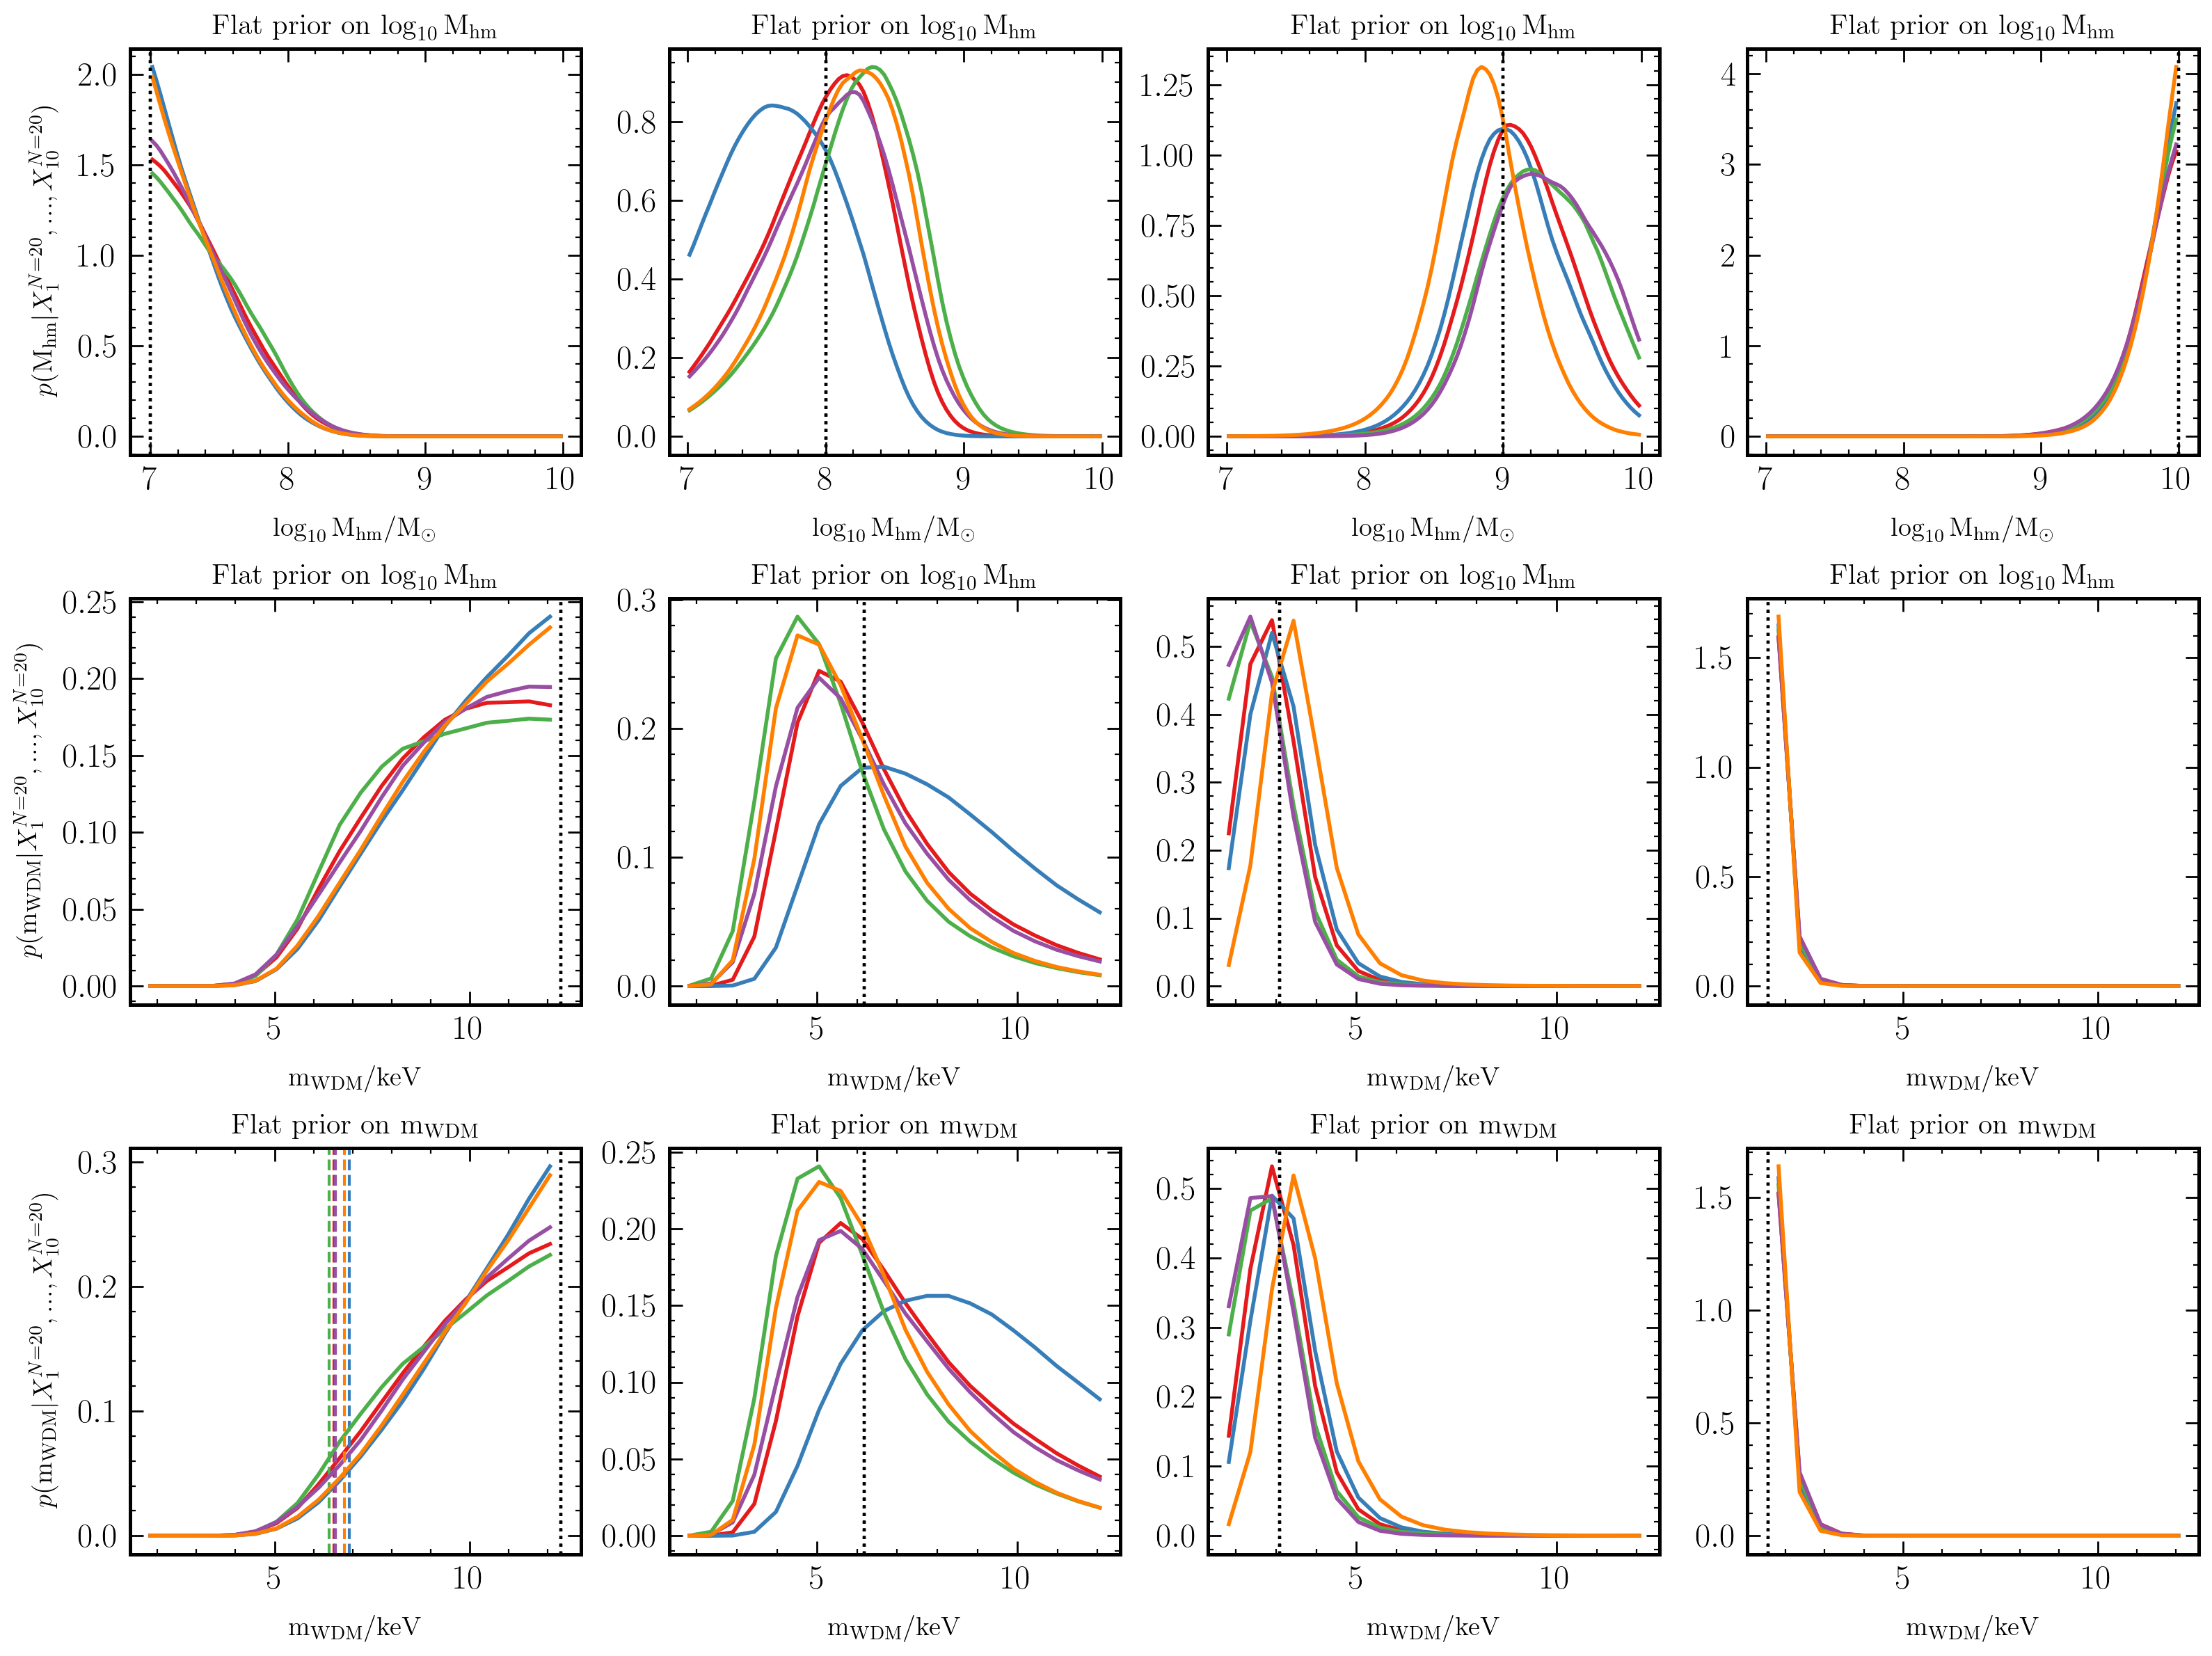
\includegraphics[width=\linewidth]{GL-wdm_results.png}
	\caption{\textit{Top:} We show five examples of combined posterior of $M=10$ sets of $N=20$ observations in terms of the cutoff mass (as the second row in Figure~\ref{fig:mhm_results}). The dotted black line represents the true input value of the half mode mass with which we have generated the analyzed mock observations ($10^7, 10^8, 10^9,  10^{10} \ \si{\solmass}$). \textit{Middle:} Same results as shown in the first column but for the \gls*{wdm} mass. The dotted black line represents the true value of the WDM mass with which we have generated the analyzed mock observations, given the mapping between \gls*{dm} cutoff and \gls*{dm} mass in Section~\ref{subsec:free-streaming}. The WDM mass posteriors assume a flat prior on the cutoff mass. \textit{Bottom:} Same results as shown in the first column but for the \gls*{wdm} mass and assuming a flat prior on the latter. In the first plot of the row, we show for the five examples the expected 95\% credible lower limit on the WDM mass for the highest value of our prior distribution.}
\label{fig:wdm_results}
\end{figure*}

Furthermore, we can translate the constraints we obtain on the cutoff mass to constraints on the WDM mass given the mapping between those two quantities defined in Section~\ref{subsec:free-streaming}. In Figure~\ref{fig:wdm_results} we show  our results for the \gls*{wdm} mass. Each column corresponds to a different cutoff mass input value, so a different WDM mass. In the first row, we plot five examples of the combined posterior density for $\log_{10}\mhm$ of $M=10$ sets of $N=20$ observations. In the second row, we show the corresponding color-coded five examples for $m_{\mathrm{WDM}}$. In this case, we just transform the posterior from the first row using the parameterization shown in Section~\ref{subsec:free-streaming}, so we assume a flat prior on $\log_{10}\mhm$. Finally, in the last row, we show the WDM mass posterior densities assuming a flat prior on the latter. The posteriors in the second and third row are not actually the same because a flat prior $\log_{10}\mhm$ is different from a flat prior on $m_{\mathrm{WDM}}$.

\subsection{Credible interval testing}
\label{subsec:test}

\begin{figure}
    \centering
    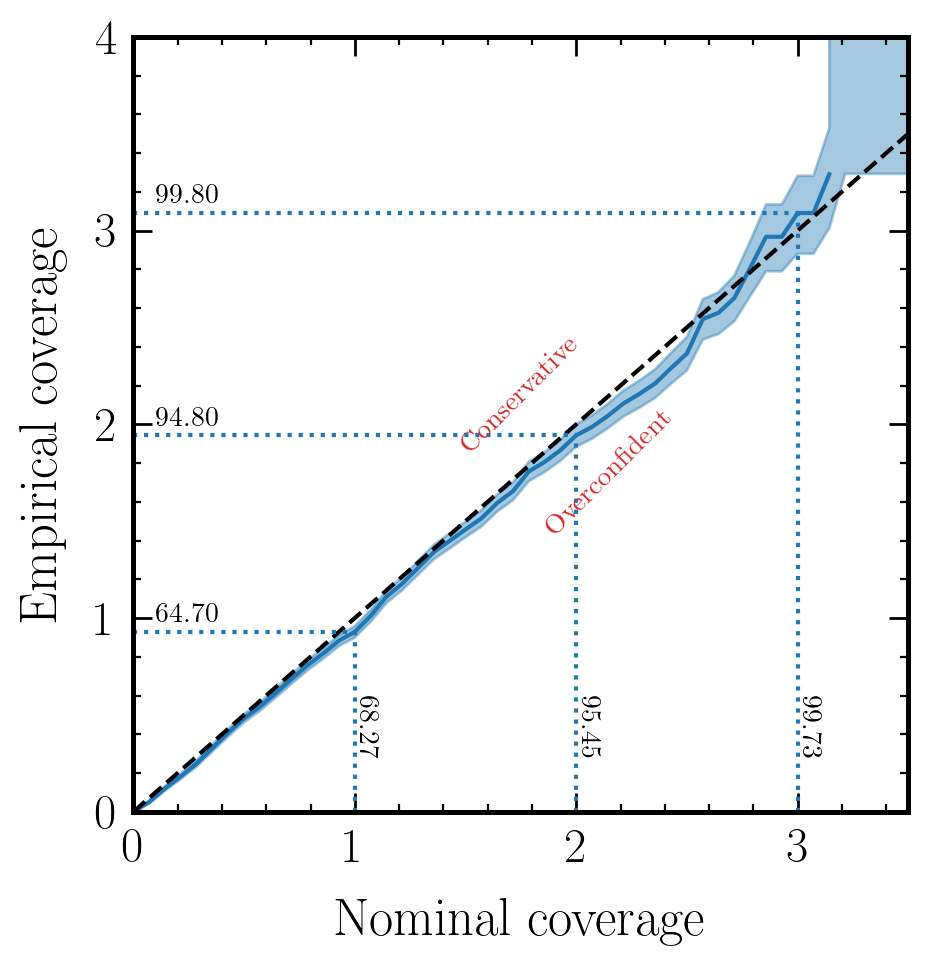
\includegraphics[width=0.5\linewidth]{GL-coverage.png}
    \caption{Empirical versus nominal expected coverage probabilities for the cutoff mass inference network. In case the line lies above (below) the black dashed diagonal line, the credible intervals are conservative (overconfident) and contain the true value with a frequency higher (lower) than nominally expected. We show the empirical (nominal) probabilities as horizontal (vertical) text.
}
\label{fig:coverage}
\end{figure}

We would like to directly test and validate the statistical behavior of our inference results by determining the expected coverage of the ratio estimator produced by the network, as described in Section~\ref{subsec:tmnre-test}. The goal is to compare the nominal and empirical expected coverage probabilities of estimated Bayesian credible intervals, which should coincide for a well-calibrated estimator. For the statistical formalism and definition of credible region and expected coverage probability, we refer the reader to Ref.~\cite{Hermans:2021rqv}. In brief, an ideal estimator has matching empirical and nominal expected coverage, a conservative one predicts lower credibility than empirically obtained, and an overconfident one has higher nominal than empirical credibility. In plots like Figure~\ref{fig:coverage}, the line for an ideal ratio estimator should perfectly align with the diagonal, whereas for a conservative (overconfident) estimator, it will lie above (below) the diagonal.
In combination with visually checking the posteriors, this test supports the accuracy of the posterior estimator and is also particularly useful when one does not have access to the ground truth against which to compare the results.
In Figure~\ref{fig:coverage} we show the empirical versus nominal expected coverage probabilities for the cutoff mass inference network. We can see that the inference network for the half-mode mass has converged with good expected coverage. 


\section{Discussion}\label{sec:sl-discussion}

In this section, we discuss the improvements to the model and inference question which need to be addressed before we can safely apply our pipeline to the analysis of real data. 

First, we have neglected effects such as inadequate \emph{lens light} subtraction and assumed the lens light to be known (this will be accounted for in Chapter~\ref{cha:anre}). Regarding the \emph{noise} model, we did not account for correlated pixel noise due to instrumental effects including the telescope's \gls*{psf}, multi-band observations, drizzling  (\eg~see Ref.~\cite{Wagner-Carena:2022mrn}), and even complex noise with an unknown likelihood function.

In this work, we have employed an analytic parameterization (the Sérsic profile) as a lensed source light distribution model, which is adequate to analyze low-resolution images. However, to accurately model higher-fidelity lensing observations, such as those from on-going (\eg~HST) and future (\eg~JWST, ELT, SKA) telescopes, more \emph{complex source models} need to be employed. Existing models, in order of complexity, are regularized pixellation of the source plane (see, \eg, \cite{Suyu:2006fd, Karchev:2021fro, Vegetti:2008eg}), source modeling through basis functions (\eg~shapelets \cite{Birrer:2018xgm} or wavelets \cite{Galan:2020mnn}) attached to the source plane, and deep learning approaches (see, \eg, Refs.~\cite{Adam:2022esz, Morningstar:2019szx}).
The ability to accurately and precisely reconstruct the complex morphology of strong-lensing sources is of the utmost importance, as to disentangle the source surface brightness inhomogeneities from the percent-level fluctuations introduced by substructures in the lens. We anticipate that using sources with more complex morphologies will result in higher sensitivity to the DM cutoff mass, provided that it is possible to model these sources. In fact, the residuals between the image of an extended source lensed by the total lens potential (accounting for substructures), and that of the same source lensed only by the main lens component are proportional to the gradient of that source evaluated in the image plane \cite[Equation 16]{Cyr-Racine:2019aa}. 

Regarding \gls*{wdm} modeling, validation of our smoothing scheme (\autoref{subsubsec:smoothing}) is required to accurately account for \gls*{dm} free-streaming effects. Moreover, we should account for uncertainties due to the assumed halo density profile by considering different \gls*{dm} distributions around galaxies (see, \eg, Ref.~\cite{Salucci:2018aa} for a review). We note that, thanks to its flexibility, our pipeline can incorporate any arbitrary \gls*{dm} model, as long as it specifies the form of the \gls*{hmf} and the density profiles of individual substructures. 
 
Finally, we would like to draw the reader's attention on the fact that in our modeling we assume that the halo mass of the lens is known exactly from its Einstein radius (see \autoref{subsubsec:sl-model-sub}). 
This is a strong assumption that has as a consequence the separation of substructure parameters $\pp$ and lens parameter $\plens$ once we marginalize the posterior probability over the halo mass in Equation~\eqref{eq:model}.
In particular, the second inference question we have addressed in this work in Section~\ref{sec:results-pop}, constraining the cutoff mass of the subhalo mass distribution, is then a simplified version of the real one, which is to simultaneously determine the halo mass and subhalo mass distribution of the lenses from real data (see, \eg, Ref.~\cite{Birrer:2017rpp}). 

While this work used simple mock lenses, \gls*{tmnre} makes it possible to add realism and parameters to a simulator without significantly altering the inference procedure, or necessarily increasing the simulation budget \cite{Cole:2021gwr}. It should therefore be straightforward to incorporate these various complexities we ignored in this work without fundamentally modifying the inference pipeline. 

%Throughout this study, we have made a number of simplifying assumptions for the, halo mass of the lens, source light profile, and substructure models. We have also neglected effects such as inadequate lens light subtraction, realistic \gls*{psf} modeling, and correlated pixel noise due to effects including the telescope's \gls*{psf}. Before this analysis pipeline can be safely extended to real observations, these assumptions need to be correctly addressed, as discussed in Section~\ref{sec:discussion}. 


\section{Conclusions}\label{sec:sl-conclusions}

Measuring the collective properties of \gls*{dm} halos on sub-galactic scales by means of their gravitational effect is an important probe of the fundamental nature of \gls*{dm}. One of such probes, strong gravitational lensing, has sparked much interest over the last few years. Moreover, the development of fast and accurate techniques to extract information from strong lensing images is well motivated by the wealth of new high-resolution strong lensing observations that will become available in the near future.

In this work, we have presented the first step towards a new neural simulation based inference pipeline (Chapter~\ref{cha:sbi}) to analyze present and future strong gravitational lensing systems in order to constrain the cutoff in the \gls*{dm} \gls*{hmf}, and so the \gls*{dm} mass (Section~\ref{sec:sl-results}). To this end, we have used a recent machine learning development, \gls*{tmnre}, that makes it possible to \textit{target} the analysis to a specific observation rather than amortize over all possible variations in lensing systems, making inference more efficient and precise. Thanks to \gls*{tmnre}, we overcome the computational challenges of traditional \gls*{mcmc}, nested sampling and trans-dimensional \gls*{mcmc} methods, by directly learning the marginal posterior for the parameter of scientific-interest from the observation. Moreover, \gls*{tmnre} leverages neural networks to directly learn the best summary statistic possible from the full input data, without having to compress the observation into hand-crafted summary statistics, like for \gls*{abc} frameworks. The method is applicable to simulators with unknown likelihood functions and large or even variable numbers of input parameters. Lastly, the resulting inference networks can be poked and prodded to confirm they are statistically well-behaved.
This work is then a step forward towards making the analysis of strong lensing images for \gls*{dm} science faster, more efficient, and more accurate. 

\mbox{}

Our key results can be summarized as follows:

\noindent\textbf{\gls*{tmnre} enables direct marginal inference.} Thanks to marginalized inference, the \gls*{tmnre} based analysis is able to correctly propagate the lens and source parameters uncertainties, and  account for the presence of a population of substructures, when estimating the marginal posterior of interest.

\noindent\textbf{\gls*{tmnre} enables direct targeted inference.} Thanks to our targeted approach, we are able to correctly estimate the lens and source parameters uncertainties, and use the final lens and source parameters truncated proposal distributions (see Section~\ref{subsec:constrain}) to generate a targeted training dataset in order to infer the \gls*{dm} cutoff. 

\noindent\textbf{\gls*{tmnre} enables statistical checks.} Since the inference networks learned by \gls*{tmnre} are locally amortized over a range of potential observations, we were able to test their statistical consistency. Our checks confirm that \gls*{tmnre} on average produces posteriors with the correct width (see \eg~Figure~\ref{fig:coverage}). Such tests would be extremely expensive with likelihood-based inference since they would require rerunning the sampling machinery on numerous mock observations.
  
\noindent\textbf{\gls*{tmnre} enables hierarchical inference.} We demonstrated that our framework is able to statistically extract the \gls*{dm} cutoff mass signal from a population of small-scale dark matter halos in the $[10^7,\ 10^{10}]\ \si{\solmass}$ mass range, by performing hierarchical inference on up to 200 observations (Section~\ref{subsec:dm} and Figure~\ref{fig:mhm_results}). A cutoff mass posterior translates into a posterior on the \gls*{wdm} mass, given the mapping in Section~\ref{subsec:free-streaming}. What we find is an expected 95\% credible lower limits around 6.5 $\si{\keV}$ in the case of the scenario closest to \gls*{cdm} (see the bottom left panel in Figure~\ref{fig:wdm_results}), given the adopted prior and the various assumptions discussed in Section~\ref{sec:sl-discussion}. 

%Measuring the properties of both individual \gls*{dm} halos and of a population of dark substructures on sub-galactic scales is an important probe of the fundamental nature of \gls*{dm}. However, extracting their parameters from observations is difficult for a myriad of reasons, including the fact that lenses contain multiple perturbers (sub-/\gls*{los} halos). In this work we demonstrated that \gls*{tmnre} enables analyses of individual perturbers' properties in scenarios where the application of likelihood-based methods is difficult or infeasible. The key strength of \gls*{tmnre} is its ability to directly learn marginal posterior functions for a set of scientifically-interesting parameters from simulated data. By truncating the range of parameters used to generate the simulations, \gls*{tmnre} enables precision inference of individual observations using a targeted set of training data. This enables the previously-intractable marginalization over large perturber populations. Furthermore, the method is applicable to simulators with unknown likelihood functions and large or even variable numbers of input parameters. The resulting inference networks can be poked and prodded to confirm they are statistically well-behaved.

\mbox{}

In this work, we have demonstrated that, in principle, the \gls*{dm} cutoff mass signal can be statistically extracted from a population of small-scale dark matter halos by a neural network using \gls*{tmnre}.
A part from the possible framework improvements discussed in Section~\ref{sec:sl-discussion}, an interesting direction for further work is the use of \gls*{tmnre} for model comparison. While here our ratio estimators were trained to compute the likelihood-to-evidence ratio, as pointed out in Ref.~\cite{Hermans:2019ioj} it is possible to learn other ratios of densities. In particular ratio estimators can be used to learn the Bayes factor for assessing the strength of the evidence for different models. This could be used to determine whether an image contains a perturber or not, and to map the minimum-detectable perturber mass as a function of its position.

Overall, we believe using \gls*{tmnre} to measure dark perturbers' population parameters as described in this work provides a promising path towards uncovering the identity of dark matter.




%%%

%\section*{Acknowledgements}
%We thank Benjamin Kurt Miller and Elias Dubbeldam for helpful discussions. We thank the anonymous referee for a careful reading and helpful comments.
%
%This work is part of a project that has received funding from the European Research Council (ERC) under the European Union’s Horizon 2020 research and innovation program (Grant agreement No. 864035 -- UnDark).
%
%A.C. received funding from the Netherlands eScience Center (grant number ETEC.2019.018) and the Schmidt Futures Foundation.
%C.C. acknowledges the support of the Dutch Research Council (NWO Veni 192.020).
%
%This work was carried out on the Lisa Compute Cluster at SURFsara. We acknowledge the use of the \texttt{python} \cite{python} modules, \texttt{matplotlib} \cite{Hunter:2007ouj}, \texttt{seaborn} \cite{Waskom:2021psk}, \texttt{numpy} \cite{Harris:2020xlr},  \texttt{scipy} \cite{Virtanen:2019joe}, \texttt{AstroPy} \cite{Astropy:2013muo}, \texttt{PyTorch} \cite{pytorch}, \texttt{Pyro} \cite{pyro}, \texttt{tqdm} \cite{tqdm}, and \texttt{jupyter} \cite{jupyter}.
%
%\section*{Data Availability}
%The data underlying this article will be shared on reasonable request to the corresponding author.

%%%%%%%%%%%%%%%%% APPENDICES %%%%%%%%%%%%%%%%%%%%%

%
\chapter{Scalable inference with autoregressive neural ratio estimation} \label{cha:anre}

In recent years, there has been a remarkable development of \gls*{sbi} algorithms, and they have now been applied across a wide range of astrophysical and cosmological analyses. There are a number of key advantages to these methods, centered around the ability to perform scalable statistical inference without an explicit likelihood. In this chapter, we propose two technical building blocks to a specific sequential \gls*{sbi} algorithm, \gls*{tmnre}. In particular, first we develop autoregressive ratio estimation with the aim to robustly estimate correlated high-dimensional posteriors. Secondly, we propose a slice-based nested sampling algorithm to efficiently draw both posterior samples and constrained prior samples from ratio estimators, the latter being instrumental for sequential inference. To validate our implementation, we carry out inference tasks on three concrete examples: a toy model of a multi-dimensional Gaussian, the analysis of a stellar stream mock observation, and finally, a proof-of-concept application to substructure searches in strong gravitational lensing. 

\textit{This chapter is based on work from \cite{AnauMontel:2023stj}.}


\section{Introduction} \label{sec:anre-intro}

 Our understanding of the universe has the potential to be revolutionized by the exponentially growing influx of high quality data from current and upcoming astrophysical or cosmological surveys~\cite{DiValentino:2020vhf}. Data from current and near-future facilities (\eg~Euclid~\cite{EUCLID:2011zbd}, JWST \cite{Gardner:2006ky}, Rubin-LSST \cite{LSSTDarkEnergyScience:2012kar}, ELT \cite{Neichel:2018aa}, Gaia \cite{Prusti:2016aa}, SKA \cite{Lazio:2009aa}, CTA \cite{Knodlseder:2020onx}) will exceed the peta- and exabyte threshold. Given this status, it is crucial for the community to develop innovative data analysis pipelines, statistical algorithms, data compression techniques, and search pipelines. These will need to handle not only the escalating amount of data, but also its increasing resolution, which directly translates into growing model complexity.

In general, to obtain information about physical models from the data, one has to solve the ``inverse problem", \ie~given an observation, the goal is to infer the parameters of a specific model (or set of models) that are most likely to have generated it. The main tools to solve inverse problems for modern astrophysical and cosmological data analysis have been sampling-based inference methods like \gls*{mcmc} \cite{Metropolis:1953am, Hastings:1970aa} and nested sampling \cite{Skilling:2006gxv, Feroz:2008xx, Handley:2015fda} techniques. However, these methods often rely on approximate likelihoods, and the time needed to reach convergence scales poorly with the dimensionality of the explored parameter space. More modern methods are taking up this latter challenge, including gradient-based algorithms such as Hamiltonian Monte-Carlo~\cite{Duane:1987de}, or slice-sampling techniques~\cite{Neal:aa, Handley:2015fda}.

Novel techniques in the field of \gls*{sbi} are starting to overcome these challenges (for a recent review see Ref.~\cite{Cranmer:2019eaq}), and have recently gained significant popularity due to a number of appealing features (see \eg~Refs.~\cite{Alsing:2018eau, Alsing:2019xrx, Lemos:2022kua, Dax:2021tsq, Wagner-Carena:2020yun, Coogan:2022cky, Legin:2022ovl, Alvey:2023pkx, Bhardwaj:2023xph, Karchev:2022xyn, Brehmer:2019jyt, Zhao:2022ren,Cole:2021gwr} for examples of method development and applications across cosmology and astroparticle physics). First of all, \gls*{sbi} methods do not require an explicit model of the data likelihood, but instead access its information implicitly via a stochastic simulator, which maps input parameters to data. Secondly, \gls*{sbi} techniques are able to directly target marginal posteriors for the parameters of interest \cite{Alsing:2019xrx, Jeffrey:2020itg}, which typically improves scalability with the dimensionality of the parameter space. This is because an arbitrarily large number of nuisance parameters can be included whilst targeting the same set of parameters of interest.\footnote{It is important to note that if all parameters contribute equally to the data variance, the implicit data distribution will become noise-dominated. Thus, when referring to scaling to arbitrary number of variables, the data variance is implicitly kept fixed. This limit remains a challenge for sampling-based methods, but is tractable in the \gls*{sbi} framework.} Lastly, sequential \gls*{sbi} approaches that continuously use the acquired inference knowledge to guide the simulator into the relevant part of the parameter space through active learning, have been shown to be particularly simulation efficient \cite{Lueckmann:2021aa}.

Whilst there are a wide range of \gls*{sbi} algorithms (we refer the reader to Section~\ref{subsec:sbi} for a broad overview), the main focus of this work will be \gls*{tmnre} \cite{Miller:2020hua, Miller:2021aa}. This is a sequential implementation of the general neural ratio estimation technique \cite{Hermans:2019ioj} that composes well with marginalisation. In essence, neural ratio estimation trains a neural network to approximate the posterior-to-prior ratio by solving a binary classification problem (for more details see Section~\ref{subsec:tmnre-nre}).
\Gls*{tmnre} has been shown to be successful in a number of different physics applications, such as cosmic microwave background analyses \cite{Cole:2021gwr}, strong lensing image analysis \cite{Montel:2022fhv, Coogan:2022cky}, supernovae Ia cosmology \cite{Karchev:2022xyn}, gravitational wave parameter inference \cite{Bhardwaj:2023xph, Alvey:2023naa}, along with other applications \cite{Gagnon-Hartman:2023soa, Saxena:2023tue, AnauMontel:2022ppb, Alvey:2023pkx}.

So far, \gls*{tmnre} applications have focused on estimating low-dimensional ($d \lesssim 2$) marginal posteriors for the parameters of interest. This choice was motivated by the fact that directly targeting these low-dimensional marginal posteriors alleviates sampling problems associated with high dimensionality, whilst still maintaining much of the information relevant for scientific conclusions. 
Nevertheless, there are situations when focusing on low-dimensional marginal posterior estimates makes \gls*{tmnre} inherently inefficient, for example when the marginals of interest are highly correlated (or multi-modal). In these cases it is therefore necessary to produce accurate high-dimensional joint estimates to account for these correlations, since higher-dimensional structure can be obscured by low-dimensional projections. This limitation becomes especially relevant for the sequential aspect of the algorithm, which cannot leverage the information regarding the correlations while guiding the simulations. However, the necessity for high-dimensional joint estimates clashes with one know failure mode of density ratio estimators, the so called ``density-chasm problem", described in Ref.~\cite{Rhodes:2020aa}. In essence, density ratio estimators can fail whenever the gap (in the sense of Ref.~\cite{Rhodes:2020aa}) between the two densities is large, since the binary classifier can obtain almost perfect accuracy with a relatively poor estimate of the density ratio. This problem is exacerbated in high-dimensions. 

The present work is a step forward towards addressing these competing limitations. Here, we propose two new building blocks of the \gls*{tmnre} framework: an \emph{autoregressive} implementation of neural ratio estimation for scalable, high-dimensional (marginal) posterior inference, and a \emph{slice-based nested sampling algorithm} to efficiently draw not only posterior samples, but also constrained prior samples. The latter set of samples, as was discussed in Section~\ref{subsec:tmnre-t}, are necessary for \gls*{tmnre}'s implementation of active learning. 

In recent years, autoregressive models have shown great potential in scaling to high-dimensional distribution estimation problems, see \eg~Refs.~\cite{Germain:2015yft, Uria:2016aa, Papamakarios:2017tec}. The term ``autoregressive" originates from the time-series modeling literature, where it refers to the practice of using previous time-step observations to predict the value at the current time step. Autoregressive models function in a similar fashion by decomposing a $d$-dimensional joint density into a product of $d$ 1-dimensional conditional distributions, as in Equation~\eqref{eq:anre-autoregressive}. An autoregressive model is then defined by the parameterization of all $d$ conditionals.

We introduce the slice sampling component because neural ratio estimators do not come with sampling functionalities. In general, to sample from the estimated (marginal) posterior, we require Monte Carlo sampling algorithms, especially in high dimensions. Moreover, we are interested in obtaining constrained prior samples for the purposes of active learning. In this context, whilst nested sampling was primarily born as a general purpose integration algorithm in high-dimensions, it has primarily been applied to perform Bayesian inference, in particular to estimate the Bayesian evidence and the posterior. Interestingly, at the heart of nested sampling algorithms resides also the problem of constrained prior sampling \cite{Ashton:2022grj}. Motivated by the success of slice-based nested samplers \cite{Neal:aa, Handley:2015fda}, we implement a custom slice sampler to draw \emph{both} posterior and constrained prior samples.  

\vspace{10pt}
 The structure of this chapter is as follows. We introduce this work's main contribution: autoregressive neural ratio estimation and prior truncation through slice-based nested sampling, in Section~\ref{sec:anre-method}. In Section~\ref{sec:anre-experiments}, we present results on a toy example, and applications to stellar streams and substructure parameter inference in strong gravitational lensing images, which initially motivated the development of the presented tools. Finally, we provide some discussion regarding possible limitations and outlook, concluding in Section~\ref{sec:anre-conclusion}. 

\vspace{10pt}
 \textbf{Code.} We release a publicly available implementation of the autoregressive ratio estimator model in the \gls*{tmnre} package \texttt{swyft}\footnote{\url{https://github.com/undark-lab/swyft}}, and an implementation of the slice-based nested sampler in \texttt{torchns}\footnote{\url{https://github.com/undark-lab/torchns}}.


\section{Methodology} \label{sec:anre-method}

 Up to now, applications of \gls*{tmnre} have typically focused on estimating low-dimensional ($d \lesssim 2$) marginal posteriors. On the other hand, whilst correlations between two parameters can always be estimated by training an appropriate ratio estimator, doing this for all pairwise combinations of a large number of parameters becomes quickly infeasible. Furthermore, even if it were done, two-dimensional correlations do not provide any information about higher order correlations since they are just projections. In certain scenarios, this might be crucial for calibrating the quality and accuracy of the inference methods and strongly motivates the development of techniques able to robustly estimate higher-dimensional posterior distributions.

As discussed in Section~\ref{sec:anre-intro}, however, there are challenges related to both the estimation of high-dimensional ratios and subsequently sampling from them. Here, we propose two new building blocks of the \gls*{tmnre} framework to address these issues: \emph{autoregressive \gls*{nre}} for scalable, multi-dimensional (marginal) posterior estimation, and \emph{slice sampling} to efficiently sample from a multi-dimensional posterior and truncated prior.\footnote{This work has been informed by private communications surrounding a complementary paper in preparation \cite{PolySwyft}.}

\subsection{Autoregressive Neural Ratio Estimation} \label{subsec:anre-anre}

 Across the various \gls*{sbi} techniques, autoregressive models have been developed in the context of density estimation algorithms, NPE~\cite{Uria:2016aa, Papamakarios:2017tec} and NLE~\cite{Papamakarios:2018aa}, and have been shown to be among the best performing density estimators~\cite{Lueckmann:2021aa}. They have been successfully applied to the Dark Energy Survey and global 21cm signal experiments~\cite{Bevins:2022qsc}, and for deep generative models for galaxy image simulations~\cite{Lanusse:2020aa}.

In a nutshell, autoregressive models turn the estimation of a $d$-dimensional joint density into the estimation of $d$ 1-dimensional conditional densities using the chain rule of probability
\begin{equation}\label{eq:anre-autoregressive}
    p(\interest \mid\data) =  p(\theta_1\mid\data) \prod_{i=2}^d p(\theta_i\mid\data, \interest_{1:i-1})\;,
\end{equation}
where we have introduced the compact notation $\interest_{1:i-1} \equiv \{\theta_1, ..., \theta_{i-1}\}$. One can thus define an autoregressive model simply by specifying a parameterization of all $d$ conditionals.

Within the NRE framework, it is also possible to perform \emph{conditional inference}. In this case, the binary classifier must be informed about the value of the parameters we want to condition over. More specifically, in order to learn the conditional posterior for parameter $\theta_i$ given parameter $\theta_j$ (with $j \neq i$), the binary classifier will be shown as positive training example $\data, \theta_j, \theta_i \sim p(\data, \theta_j, \theta_i)$ and as negative training examples $\data, \theta_j, \theta_i \sim p(\data, \theta_j)p(\theta_i)$. We can then express the conditional ratio trained on $(\data, \theta_j\}, \theta_i)$ pairs as
\begin{equation}
    \label{eq:ratio_conditional}
    r(\theta_i;\data \theta_j) \equiv
    \frac{p(\theta_i \mid \data, \theta_j)}{ p(\theta_i)} \, .
\end{equation}
It is possible to condition more than one parameter $\theta_i$ on more than one variable $\theta_j$ just by correctly passing to the classifier positive and negative training examples as defined above. 

We can then use 1-dimensional versions of these ratio estimators, conditioned on multiple variables, to implement autoregressive \gls*{nre}. More in details, one way to estimate our ratio of interest $r(\interest; \data)$, as defined in Equation~\eqref{eq:sbi-ratio}, auto-regressively is by considering the following components. The first quantity, $A$, estimates the ratio between the joint posterior distribution and the independent marginal priors,
\begin{equation} \label{eq:anre-A}
\begin{split}
    A &= 
    \frac{p(\interest\mid \data)}{\prod_{i=1}^d p(\theta_i)} \\
    & = \frac{p(\theta_1\mid \data)}{p(\theta_1)} \prod_{i=2}^d \frac{p(\theta_i\mid \data, \interest_{1:i-1})}{ p(\theta_i)} \\
    & = 
    r(\theta_1;\data)  \prod_{i=2}^d  r(\theta_i;\data, \interest_{1:i-1}) \;.
\end{split}
\end{equation}
The second component, $B$, models the dependencies between the model parameters,
\begin{equation} \label{eq:anre-B}
\begin{split}
    B &= 
    \frac{p(\interest)}{\prod_{i=1}^d p(\theta_i)} \\
    & = \prod_{i=2}^d \frac{p(\theta_i \mid \interest_{1:i-1})}{p(\theta_i)} \\
    & = \prod_{i=2}^d r(\theta_i;\interest_{1:i-1}) \;.
\end{split}
\end{equation}
Our key quantity of interest is then obtained as 
\begin{equation} \label{eq:anre-AB}
    r(\interest;\data) = \frac{p(\interest \mid \data)}{p(\interest)} = A/B \;.
\end{equation}
It is important to highlight the role of the $B$ component in this algorithm. In the case of sequential inference, even if the initial prior distributions from which parameters are drawn are independent, the sequential proposal distribution will account for non-trivial correlations between parameters in the constrained prior region (via the condition in Equation~\eqref{eq:gamma_r}). It is therefore crucial to properly account for these correlations between parameters through $B$ since they will implicitly be present in the training data. 

Also note that in both the definitions of $A$ and $B$, we have used the notation introduced in Equation~\eqref{eq:ratio_conditional} for conditional ratios. An alternative formulation of an autoregressive model for ratio estimation that uses a single network to model both components is presented in Appendix~\ref{apx:anre-anre}.

The key advantage of autoregressive NRE lies in its ability to handle intricate dependencies among variables by focusing on one parameter at a time. In ``vanilla" NRE, for high-dimensional parameter spaces, the discriminating power of the binary classifier can be quickly saturated leading to a poor estimate of the joint density ratio. Here, the full joint distribution is modeled through 1-dimensional conditional ratios, leading to a more stable and accurate estimation of the full joint ratio. However, the presented autoregressive NRE method does inherit the generic drawbacks of autoregressive models. Perhaps the most relevant is their sensitivity to the order of the conditional probabilities, since in practice it is difficult to know which of the factorially many orders is the most efficient in each case \cite{Papamakarios:2017tec}. A possible solution was presented in \cite{Uria:2013aa}, that introduced an efficient procedure to simultaneously train an autoregressive model for all possible orderings of the variables. We will study this effect explicitly in the stellar streams example given in Section~\ref{subsec:anre-stream}. 


\subsection{Prior truncation strategies}\label{subsec:anre-truncation}

 The original prior truncation scheme proposed in the \gls*{tmnre} formalism \cite{Miller:2021aa} is a parameter-wise truncation based on 1-dimensional marginal ratio estimators. As a result, the prior gets restricted to a truncation region that has the shape of a hyper-rectangular box (``box" truncation), 
\begin{equation} \label{eq:anre-box}
     p^{(R)}_{\Gamma}(\interest) = \frac1Z \mathbb{I}(\theta_1 \in \Gamma_{\theta_1}^{(R-1)}) \times \cdots \times\mathbb{I}(\theta_d \in \Gamma_{\theta_d}^{(R-1)}) p(\interest) \,,
\end{equation}
where we have introduced the indicator function $\mathbb{I}$ which is unity on the truncated prior support $\Gamma_{\theta_i}^R$ and zero otherwise, and the normalizing constant $Z$ which can be interpreted as the fractional volume of the truncated prior.

One of the drawbacks of using this box truncation scheme is that it neglects parameter correlations. For higher ($d \gtrsim 2$) dimensional marginal posteriors, this results in the new constrained region usually containing significantly more probability mass than is actually required (see \eg~\cite{Karchev:2022xyn}).

In this section, we propose a parameter block-wise truncation scheme (``correlated" truncation) based on high-dimensional ratio estimators that accounts for correlations between parameters. This correlated truncation region is defined through a hard likelihood-to-evidence ratio constraint,
\begin{equation} \label{eq:anre-block}
    \tilde p^{(R)}_{\Gamma}(\interest) = \frac1Z \mathbb{I}(\interest \in \Gamma_{\interest}^{(R-1)}) p(\interest) \,,
\end{equation}
where $\Gamma_{\boldsymbol{\theta}}^{(R - 1)}$ is as defined in Equation~\eqref{eq:gamma_r}. In Figure~\ref{fig:anre-ns}, we show a visual comparison of the two prior truncation strategies in a simple 2-dimensional parameter space. However, following this approach brings about a new challenge that will be addressed in the next section: how does one efficiently define the boundaries of $\Gamma_{\interest}^{(R)}$ and sample from within it?

\begin{figure}[h]
	\centering
	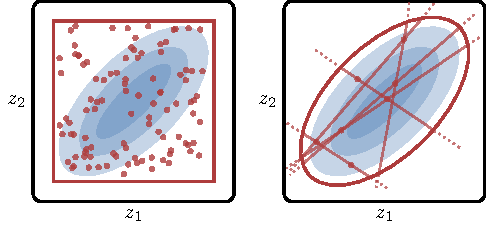
\includegraphics[width=0.8\linewidth]{TikZ/truncation_ns.pdf}
	\caption{Prior truncation strategies. We visualize in a 2-dimensional parameter space a constrained prior region using hyper-rectangular boxes as defined in Equation~\eqref{eq:anre-box} (red rectangle on the left), and a constrained prior region using hard iso-likelihood-to-evidence ratio contours as defined in Equation~\eqref{eq:anre-block} (red ellipse on the right). Sampling from hyper-rectangular boxes is equivalent to uniform sampling, whereas sampling from iso-likelihood-to-evidence ratio contours requires more sophisticated sampling algorithms. In particular, we use a slice-based nested sampler as explained in Section~\ref{subsec:anre-ns}. 
}
\label{fig:anre-ns}
\end{figure}


\subsection{Sampling from ratio estimators: posterior and constrained prior samples} \label{subsec:anre-ns}

 As discussed in Section~\ref{sec:anre-intro}, NRE does not have sampling functionalities and Monte Carlo-based sampling algorithms are used to obtain samples from the approximate posterior.\footnote{It is worth noting that this is somewhat contrary to NPE, where one can directly draw posterior samples from the normalising flow.} Moreover, we are not only interested in posterior samples, but also in how we can efficiently draw constrained prior samples from a region defined through a hard likelihood-to-evidence ratio constraint. Here, we propose utilizing a \emph{slice-based nested sampling algorithm}, as an efficient method to sample both posterior samples and constrained prior samples from the ratio estimator. Importantly, constrained prior samples can be obtained through the same nested sampling techniques. Our sampler choice is strongly inspired by the success of slice-based nested samplers in efficiently and reliably exploring high dimensional parameter spaces \cite{Handley:2015fda, Handley:2015fda}. Additionally, slice sampling was proposed in Ref.~\cite{Papamakarios:2018aa} as a sampler for NLE. 

First proposed in Ref.~\cite{Skilling:2006gxv}, nested sampling allows one to sample from high-dimensional probability densities by evolving an ensemble of live points through a high-dimensional parameter space. At the core of nested sampling algorithms is the problem of constrained prior sampling within iso-likelihood contours \cite{Ashton:2022grj}. This opens up the possibility to re-use technology developed for nested sampling for the purpose of sampling not only from the posterior, but also from the constrained prior region, as defined in Equation~\eqref{eq:gamma_r} within iso-likelihood-to-evidence ratio contours.\footnote{In traditional implementations the contours are defined by iso-likelihood levels, not iso-likelihood-to-evidence ratio levels.}

Typically, nested sampling algorithms start by drawing a collection of live points from the prior. In the current context, one evolves them by discarding the point with the lowest ratio, denoted with $r_\mathrm{min}$, and replacing it with a new point subject to the constrain $r > r_\mathrm{min}$. The remaining live points are now uniformly distributed over a compressed volume (as they are drawn from a constrained prior as in Equation~\eqref{eq:gamma_r} with $\epsilon = r_\mathrm{min}$).

The most challenging aspect of the nested sampling algorithm is drawing new live points under the hard likelihood-to-evidence ratio condition $r > r_\mathrm{min}$. One possible reliable and efficient way to do so is through slice sampling, first introduced in \cite{Neal:aa}. Starting from one randomly chosen live point, slice sampling builds a chain of proposed live points by taking sequential 1-dimensional steps in a random direction. The length of this chain controls the amount of correlation between the new live point and the initial one (for further information see Ref.~\cite{Buchner:2021kpm}).

In our slice sampling implementation, we use a number of different ploys to make our sampling scheme more efficient for the purposes at hand. Firstly, instead of a single chain, the user can define the number of slice sampling chains to draw new live points that will be run in parallel. Secondly, the sampler is implemented such that it allows vectorized evaluations of the natively GPU-based ratio estimator, which provides considerable computational speed-up. We also provide useful functionality to compute the threshold $\epsilon$ that defines the constrained prior region in Equation~\eqref{eq:gamma_r}, based on how much probability mass from the current approximate likelihood-to-evidence ratio one wants the region to include. This is relevant for setting the convergence criterion related to posterior mass that defines the iso-likelihood-to-ratio contour, as in Equation~\eqref{eq:gamma_r}. Importantly, inference errors caused by truncation arise when not enough posterior mass is included in the truncated regions, resulting in wrongly excluded parts of the parameter space of interest (for a detailed discussion and test of the impact that overly tight complex truncation induces on inference, we refer the reader to Appendix 6.10 of Ref.~\cite{Deistler:2022aa}). 
For sequential \gls*{sbi} applications, we advise the user to conservatively choose the threshold $\epsilon$ such that the truncated prior encloses the highest probability density (HPD) region that contains at minimum $99.9 \%$ (\ie~$1 - 10^{-3}$) of the probability mass. 

\paragraph*{Network stability during sampling.}
During the sampling step, numerical issues can arise because the slice sampler may evaluate the network outside of the current truncation region $\Gamma^{(R)}_{\boldsymbol{\theta}}$ when searching for new points.
In order to detail the issue, we recall our definition of $B={p(\boldsymbol \theta)}/{\prod_{i=1}^d p(\theta_i)}$, which is zero outside of the support of the joined distribution $p(\boldsymbol \theta)$. Formally, this is not a problem for the ratio $A/B$ (see Equation~\eqref{eq:anre-AB}), because that region coincides with the prior region that we truncated away in our truncation procedure (\ie~regions of very low posterior mass). In practice, during sampling, since the network in a given round $R$ has not seen training samples outside of the constrained prior $\tilde p^{(R)}(\interest)$ (see Equation~\eqref{eq:anre-block}), this can lead to estimated values of our neural likelihood-to-evidence ratio $A/B$ which are much larger than the formal expectation (indeed $B = 0$ exactly outside this region).

We solve this stability issue with the following strategy, that has no impact within the truncation bounds $\Gamma^{(R)}_{\boldsymbol{\theta}}$, and therefore on the results.
During the sampling step, the following substitution is performed in the network
\begin{equation}
    B \rightarrow \text{max}(B, \min_{\Gamma^{(R)}_{\boldsymbol{\theta}}}B). 
    % \qquad \text{in sampling round (R+1)}.   
\end{equation}
Hence, $B$ can be at minimum as small as the smallest value it can take inside the truncation bound $\Gamma^{(R)}_{\boldsymbol{\theta}}$. As a result, the substitution will never happen inside the constrained region $\Gamma^{(R)}_{\boldsymbol{\theta}}$ where the network was trained, and consequently will not have any impact on the new truncation set $\Gamma^{(R+1)}_{\boldsymbol{\theta}} \in \Gamma^{(R)}_{\boldsymbol{\theta}}$. We further emphasize that by construction, the truncation region should never expand throughout a round, so this new substitution only plays the role of fixing the stability issues outside the constrained prior.


\vspace{10pt}
 To summarise, in this section we have presented the main contributions of this work in the form of two new building blocks of the \gls*{tmnre} framework: autoregressive \gls*{nre} and a slice-based nested sampler to sample posterior and constrained prior samples from a ratio estimator. In the next section, we will apply these newly developed tools to a toy Gaussian example, as well as two astrophysical applications -- stellar streams and strong lensing.


\section{Experiments} \label{sec:anre-experiments}

 We first apply our newly developed tools to a toy multivariate Gaussian example. For more realistic settings, we consider two astrophysics problems: stellar streams parameter inference and substructure parameter inference in strong gravitational lensing observations.

\subsection{Multivariate Gaussian: scalability} \label{toy}

\begin{figure}
\centering
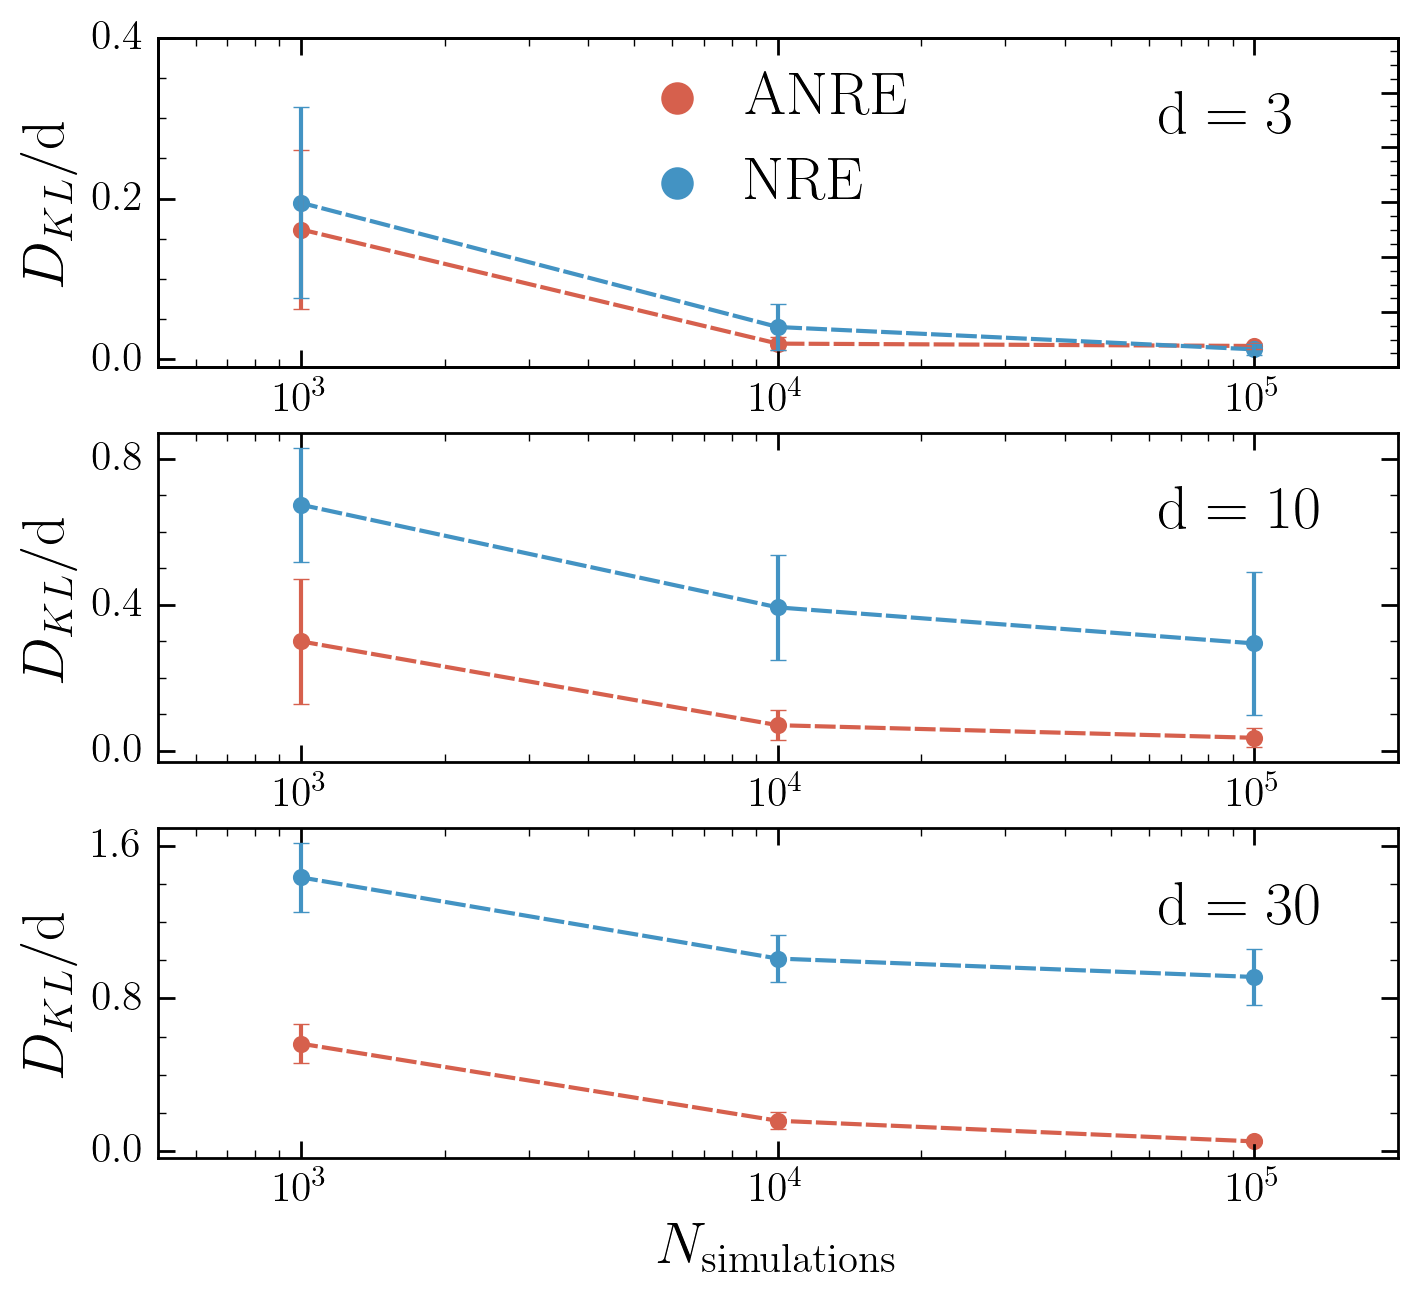
\includegraphics[width=0.7\linewidth]{ANRE-toy.png}
\caption{
 Multivariate Gaussian toy example results. In the three panels we show the KL divergence value between the analytical posterior distribution and the estimated ones from the autoregressive (ANRE, in red) a non-autoregressive (\gls*{nre}, in blue) models. The metric is shown as a function of simulation budget in three different dimensionalities ($d=3, 10, 30$). For our fixed network capacity, \gls*{nre} is able to perform as well as ANRE for high simulation budget in low-dimensional scenarios. For higher-dimensionality, the quality of posterior samples obtained from the autoregressive model matches significantly more closely the one from the analytic solution based on the KL divergence value.}
\label{fig:toy}
\end{figure}

 In this first application, we are interested in testing how the performance of ``vanilla" \gls*{nre} and autoregressive \gls*{nre} models scale with dimensionality and simulation budget. To do so, we consider a $d$-dimensional Gaussian toy model with strong correlations. The parameters $\interest \in \mathbb{R}^d$ are drawn from a multivariate normal prior $p(\interest)=\mathcal{N}(\mathbf 0, \mathbf{\Sigma_0})$, with diagonal covariance matrix $\mathbf{\Sigma_0}= 0.1 \odot \mathbf I$. The observations $\data \in \mathbb{R}^d$ are drawn from a multivariate normal likelihood $p(\data \mid \interest)= \mathcal{N}(\interest, \mathbf{\Sigma})$, with fixed covariance $\mathbf{\Sigma}$, which has correlation scales of $0.1$ for the off-diagonal entries, and $0.11$ for the diagonal ones. As a reference, we use the analytic solution for the true posterior given by Bayes' theorem.

We test \gls*{nre} and autoregressive \gls*{nre} for dimensions $d = 3, 10, 30$ and for different simulation budgets of $N_\mathrm{simulations} =10^3, 10^4, 10^5$ training data examples. Each conditional ratio in the autoregressive network is modeled with $4$ ResNet \cite{He:2015wrn} blocks with $64$ hidden features (implemented in \texttt{swyft}). The ``vanilla" \gls*{nre} network is instead modeled with a single network whose number of ResNet blocks and parameters is adjusted accordingly to match the total number of parameters in the autoregressive model. 

To compare the performance of the two models we consider the Kullback-Leibler (KL) divergence $D_\mathrm{KL}$ between the posterior estimated by each model and the analytical solution. The KL divergence is a statistical distance that measure the difference between two probability distributions; the closer it is to zero, the better agreement there is. The mean and the covariance of the estimated posterior are computed from the posterior samples of the two models, obtained with our slice-based nested sampler. 
Our results are shown in Figure~\ref{fig:toy}, where each point is the mean KL divergence of 10 different observations. The error bar represents the standard deviation of these values. In low-dimensional scenarios ($d=3$), \gls*{nre} is able to perform as well as autoregressive \gls*{nre} for high simulation budget. For higher-dimensionality, the quality of posterior samples obtained from the autoregressive model matches significantly more closely the one from the analytic solution for lower simulation budgets. In Appendix~\ref{apx:anre-toy}, we show the comparison between the analytical posterior and the estimated posterior with simulation budget $N_\mathrm{simulations} = 10^{5}$ from the two models for one observation with $d=10$.

\subsection{Stellar streams: autoregressive variable ordering} \label{subsec:anre-stream}

\begin{figure*}
    \centering
     \begin{tikzpicture}[every node/.style={anchor=center}]
        \node(a) at (8,4){ 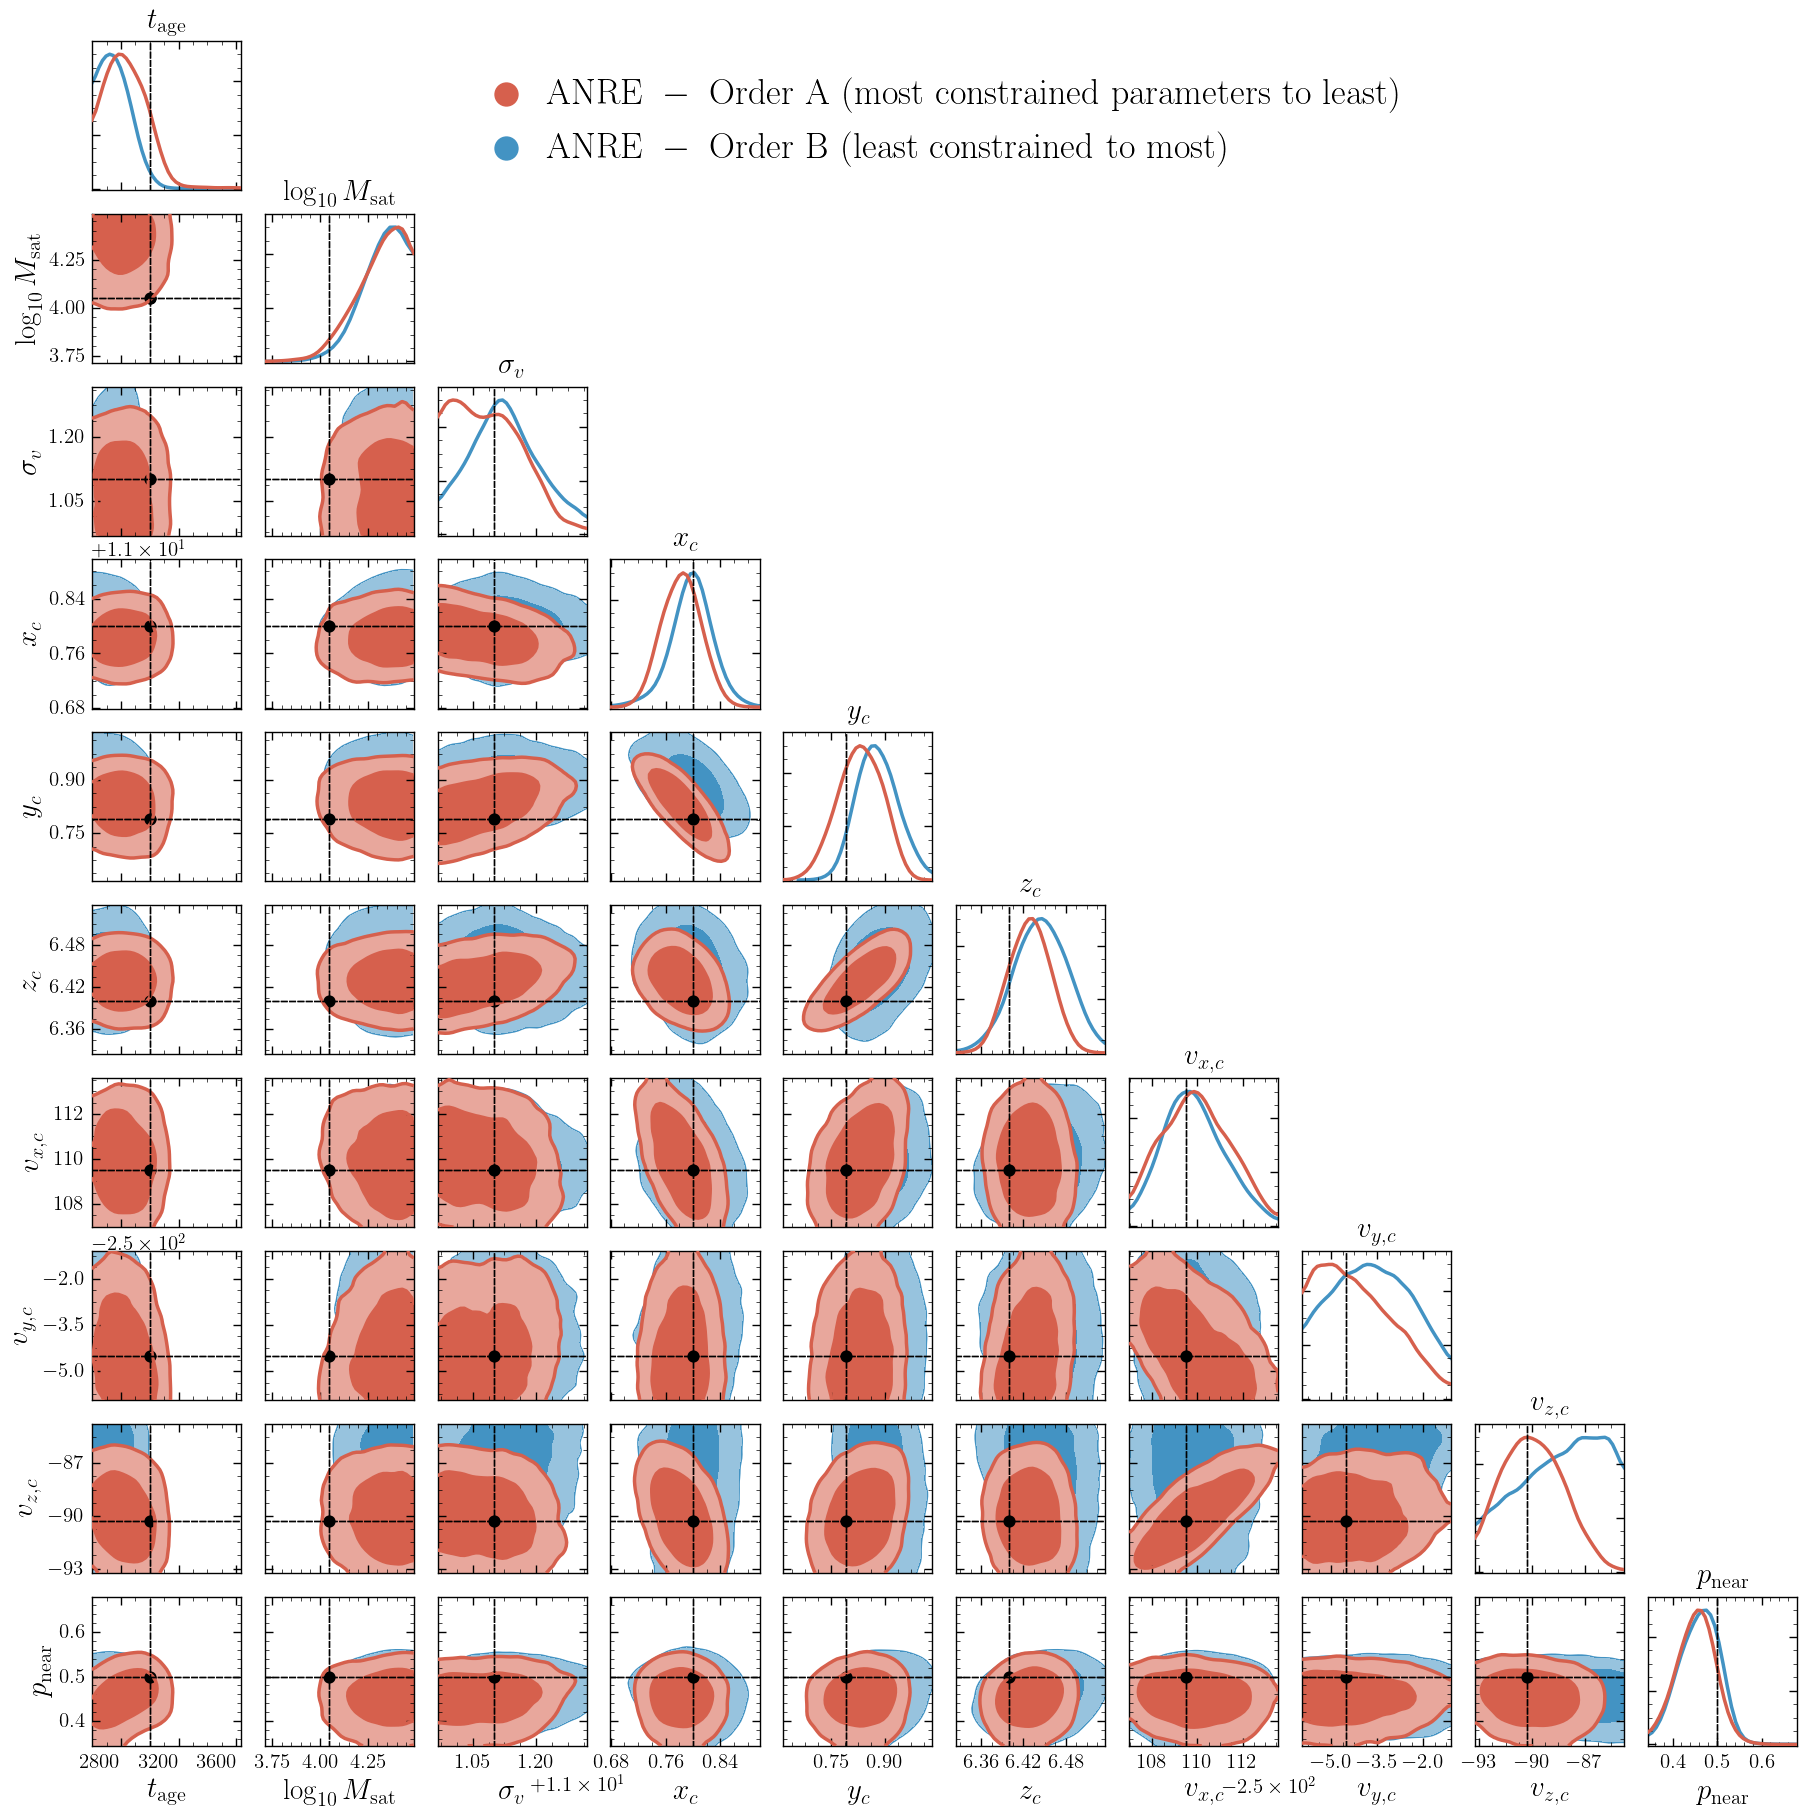
\includegraphics[width=\linewidth]{ANRE-corner_streams.png}};
        \node(b) at (12,6){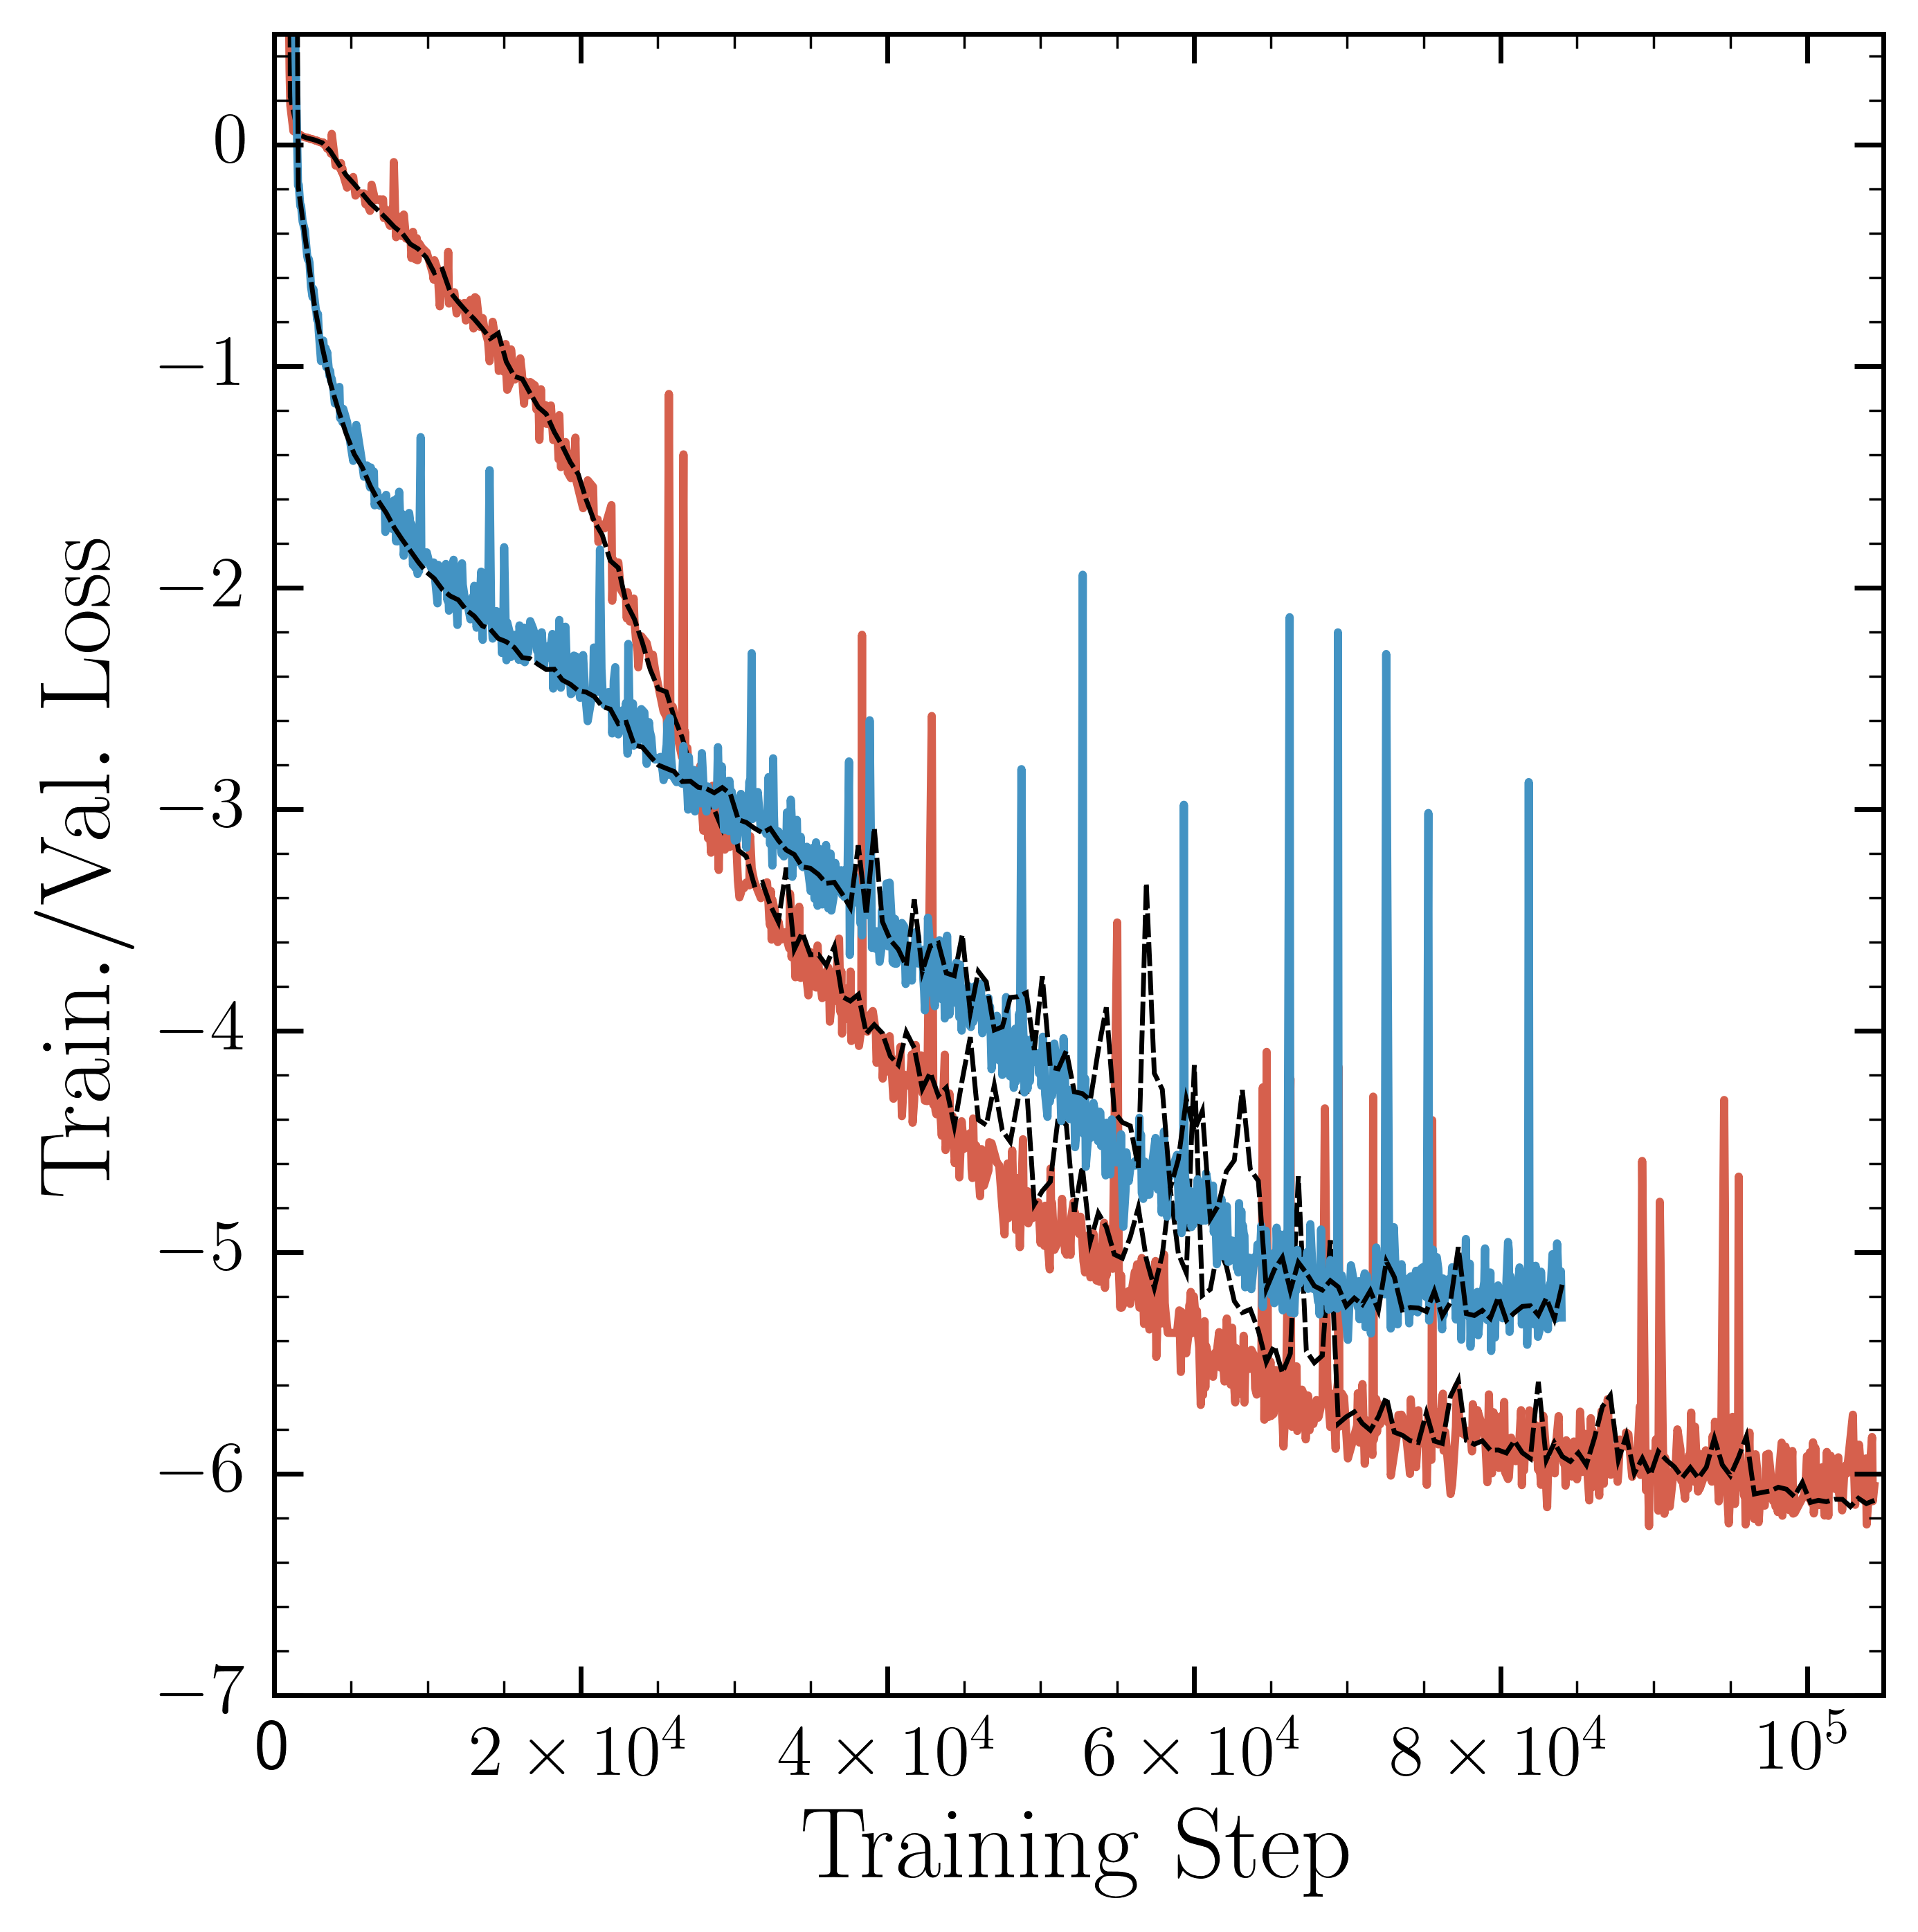
\includegraphics[height=6cm]{ANRE-loss.png}};
    \end{tikzpicture}
    \caption{Stellar streams experiment results. \emph{Corner plot:} The corner plot shows the comparison between the inference results using different parameter ordering schemes across those parameters that are constrained in the analysis (for the full set, see Appendix~\ref{apx:anre-streams}). Order A (most constrained parameters to least constrained) is shown with red contours, whilst Order B (least constrained to most) is shown in blue. We see that Order A performs marginally better in terms of precision, although the improvement is somewhat marginal. The true injected values are shown with black dashed lines and dots. \emph{Upper right inset:} This inset shows the training loss (see Equation~\eqref{eq:sbi-bce}) as a function of the number of training steps for the two orderings. We see that Order A achieves a lower value of the loss, in line with the conclusions from the corner plot. The validation loss for each case is shown with black dashed lines.}
    \label{fig:streams_loss}
\end{figure*}

 Stellar streams are very old, dynamical objects in the Milky Way that form as the result of the tidal disruption of objects such as globular clusters or small dwarf galaxies as they orbit the host. In principle, they can act as detailed tracers of the galactic potential, the disruption history and physics of the star clusters, and even possible dark substructures in the Milky Way (see \eg~Refs.~\cite{Erkal:2015kqa,Banik:2018pjp,Banik:2018pal,Koposov:2009hn,Bonaca:2014qia,Amorisco:2016evb,Bovy:2016chl,Malhan:2022nfe} for examples of the existing analyses). On the other hand, robust analysis of these objects is challenging for a number of reasons. Firstly, simulating the stream in full generality is computationally challenging, so delicate modeling choices need to be made. Secondly, the statistical properties of the resulting stream are difficult to write down explicitly in the form of a likelihood, mainly due to complicated observational effects such as membership probabilities in \eg~Gaia data \cite{Gaia:2018ydn,Gaia:2021aa}. Combined with the general simulation efficiency that has been observed with neural ratio estimation, this strongly motivates the application of \gls*{sbi} techniques to such a problem, something that has been studied in detail in Ref.~\cite{Alvey:2023pkx} (see also Ref.~\cite{Hermans:2020skz}).

In the current context, we will use the inference of stream model parameters in an identical set up to Ref.~\cite{Alvey:2023pkx} to highlight a relevant aspect of the autoregressive algorithm presented in this work. Specifically, we use the case study to highlight the implications that varying the ordering of parameters in the conditional distributions product found in Equation~\eqref{eq:anre-A} has on inference performance. The intuition that we wish to test is the following: we expect that the distribution $p(\theta_i | \data)$ is most useful to learn if $\theta_i$ is well constrained. Similarly, if $\theta_j$ is not well constrained, then adding conditional information \eg~in $p(\theta_j | \data, \interest_{1:j-1})$ can add relevant information. With this said, the expectation is that an approximately optimal ordering runs from $\theta_1$ as the most constrained parameter (relative to the prior), and $\theta_d$ as the least constrained parameter.

Given the analysis in Ref.~\cite{Alvey:2023pkx}, we have good expectations about the relative constraining power of the streams analysis on various parameters. As such, we choose two orderings: Order A which runs from most to least constrained, and Order B which runs vice versa (see Appendix~\ref{apx:anre-streams} for details). We train an autoregressive estimator in both cases to perform inference on all parameters of the model. The results of this experiment are shown in Figure~\ref{fig:streams_loss} in terms of the resulting posterior distributions, as well as the training and validation loss curves for the neural network training process. 

There are two things to note from Figure~\ref{fig:streams_loss}: firstly, the ordering of parameters does have an effect on the training procedure, with the expectation laid out above clearly realised. In other words, we see a plateauing of the optimal training and validation loss for Order B at a value that is clearly larger than the asymptotic value in the case of Order A. In addition, broadly the overall quality of posterior inference on parts of the model that are well measured is of higher quality with Order A. Together, this suggests that the general intuition regarding parameter ordering in autoregressive models holds here also. With that being said, however, we do observe that the `penalty' for choosing a non-optimal ordering is not severe, at least in this case, and high fidelity inference could be achieved by \eg~increasing the simulation budget (see Appendix~\ref{apx:anre-streams} for an example), or following the prior truncation scheme described above and iterating the simulation generation, training, and inference steps. To be clear on this last point, this example is designed to demonstrate for fixed simulation budget and fixed network architecture the impact of variable ordering. We expect in this particular case that if the prior truncation scheme is followed, the posteriors will continue to shrink and converge to the same answer. For high precision inference, we advise that on convergence, an explicit test varying the ordering is carried out to confirm that the posteriors do not shift by more than the desired sensitivity. For full technical details regarding this example, see Ref.~\cite{Alvey:2023pkx} or Appendix~\ref{apx:anre-streams}.  Also in Appendix~\ref{apx:anre-streams}, we show two other random orderings to highlight the relative insensitivity to this choice and build on the example in \autoref{toy}.

\begin{figure*}
 \begin{tikzpicture}[every node/.style={anchor=center}]
    \node(b) at (11,8){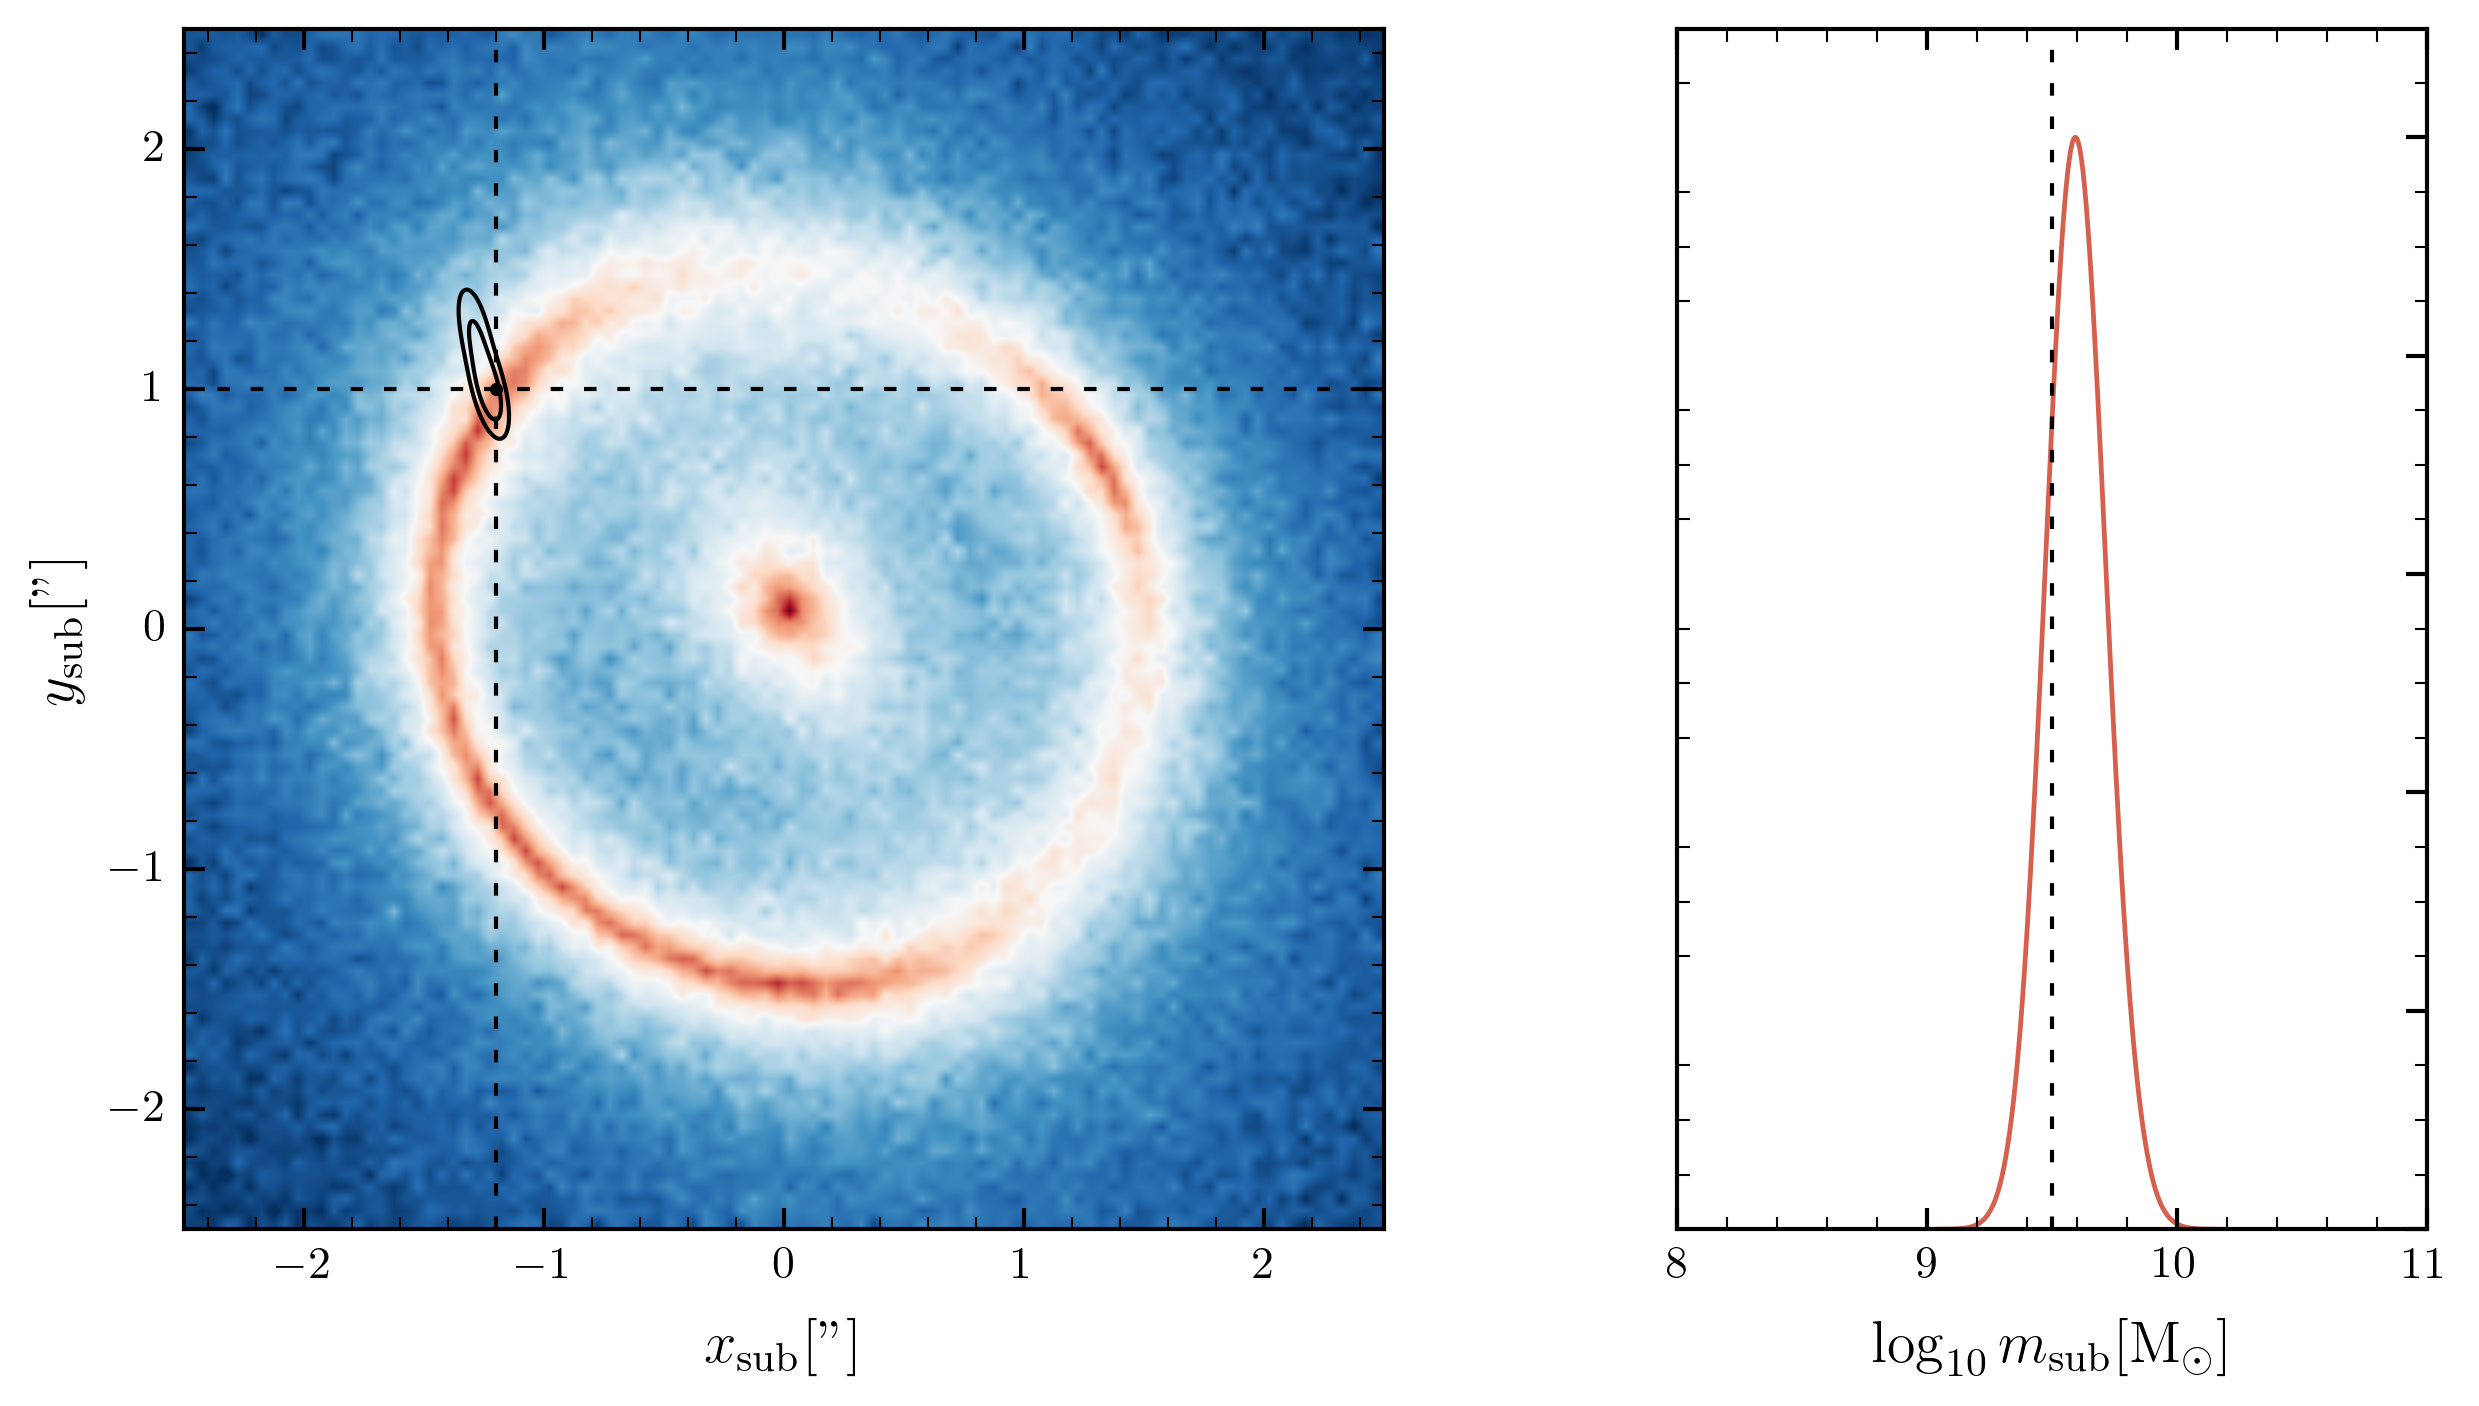
\includegraphics[height=4.5cm]{ANRE-sub_new.png}};
    \node(a) at (8,4){\includegraphics[width=\textwidth]{ANRE-corner.png}};
\end{tikzpicture}
\caption{Strong gravitational lensing experiment results. \emph{Corner plot:} The corner plot shows the comparison between the macro-model parameter inference results using the autoregressive \gls*{nre} model (ANRE, red contours) and the non-autoregressive one (\gls*{nre}, blue contours). The true values are shown with black dashed lines and dots and are shown in Table~\ref{tab:anre-lensing-params}. \emph{Upper right inset:} The inset shows the results for subhalo parameter inference for our target mock observation.
}
\label{fig:corner}
\end{figure*}


\subsection{Strong gravitational lensing: correlated truncation} \label{subsec:lensing}

 As described in Chapter~\ref{cha:lensing}, galaxy-galaxy strong gravitational lensing occurs when the paths of light rays from a background galaxy are distorted by the mass of an intervening lens galaxy before entering a telescope \cite{Meneghetti:2016aa}. This leads to extremely distorted ring-shaped images with multiple copies of the source. If a small-scale dark matter halo is present in such a system, its distortions will be localized, mostly impacting the image of the source along the nearest line of sight. As first proposed in \cite{Mao:1997ek}, by carefully analyzing the relationship between the multiple images of the source, the distortions due to a dark matter perturber can be disentangled from possible variations in the source light and its properties can be measured.

In reality, substructure parameter inference in strong gravitational lensing systems is a very challenging task for a number of reasons. In particular, the desired signal manifests as percent level variations, lensing systems are remarkably complicated, and the variance between images is high (\ie~observations are very diverse). A targeted \gls*{sbi} approach to this ``needle in a haystack" type of analysis is therefore well-motivated and has been proven successful, see \eg~Refs.~\cite{Coogan:2020yux, Coogan:2022cky}. 

For this application, we consider a lensing system with the following components: source light, lens light, lens mass distribution, and external shear (which we collectively call the macro-model); and one single subhalo. More details on the system and noise model can be found in Appendix~\ref{apx:anre-lensing}. The blending effect due to the overlap of the light emitted by the lensed source and by the lens itself complicates the interpretation and analysis of observed lensed systems, and makes it challenging to isolate and study the properties of the lensed source. This blending effect can be mitigated if multi-wavelength observations are available. Usually the lens light gets subtracted assuming the best-fit value (see \eg~Ref.~\cite{Vegetti:2012mc}). In this \gls*{sbi} application, we leave it free to vary and infer its parameters at the same time as all other components, accounting in the analysis for its uncertainties and the correlations it has with the rest of the system components.

We perform inference on the simulated target observation shown in Figure~\ref{fig:corner}, generated with the parameters in Table~\ref{tab:anre-lensing-params}. The first step in the analysis is to reduce training data variance by constraining the macro-model parameters prior. Starting from the full macro-model prior shown in Table~\ref{tab:anre-lensing-params}, we use the procedure described in Refs.~\cite{Coogan:2022cky, Montel:2022fhv} to constrain it sequentially via \gls*{tmnre} rounds using box truncation. When convergence\footnote{We define the ratio estimator to be converged when, after two consecutive rounds in which we double up the simulation budget, the constrained hyper-rectangular box prior has shrunk by less than 10\%.} is reached, we are not able to reduce any further the data variance displayed by the simulations via 1-dimensional marginal posterior estimation and box truncation.

As previously discussed in Section~\ref{subsec:anre-truncation}, a disadvantage of using hyper-rectangular boxes lies in the fact that for high-dimensional and correlated parameter spaces the constrained region contains more probability mass than required. We will now employ a parameter block-wise correlated prior truncation strategy instead of box truncation, as presented in Section~\ref{subsec:anre-truncation}. In Figure~\ref{fig:block}, we show a simple visualization of the two prior truncation strategies for this specific application.

In order to learn the macro-model parameter correlations, especially the ones between lens light and source light, we model the joint posterior of the  macro-model parameters. We train two models to estimate the macro-model joint ratio: a ``vanilla" \gls*{nre} model and the autoregressive \gls*{nre} model presented in Section~\ref{subsec:anre-anre}. We used the same simulation budget and amount of network weights (for more details regarding training and the employed neural network architecture, see Appendix~\ref{apx:anre-lensing}). In Figure~\ref{fig:corner}, we compare the posterior samples obtained from the two models using our slice-based nested sampler presented in Section~\ref{subsec:anre-ns}. It is clear that, for this application and simulation budget, autoregressive \gls*{nre} performs significantly better than \gls*{nre}, which is not able to properly model the joint macro-model parameter distribution.

\begin{figure}
	\centering
	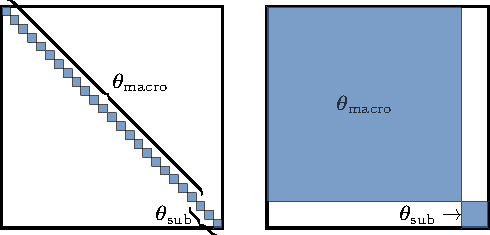
\includegraphics[width=0.8\linewidth]{TikZ/truncation_blocks.pdf}
	\caption{Prior truncation strategies. \emph{Left:} With a parameter-wise truncation strategy, each parameter gets individually constrained with boxes. \emph{Right:} Using a parameter block-wise truncation strategy, we divide the parameter space in blocks (lensing macro-model parameters $\interest_\mathrm{macro}$ and subhalo parameters $\interest_\mathrm{sub}$), depending on what dominates the data variance, and which parameters are most correlated. During sequential inference, we account for correlations between parameters in the same block through correlated truncation.}
	\label{fig:block}
\end{figure}

We then sample correlated constrained prior samples with our slice-based nested sampler. By modeling and exploiting the intricate correlations between lens light, source light, and lens parameters, instead of using a parameter-wise truncation strategy, we are able to achieve a much lower data variance. In Figure~\ref{fig:targeted_data}, we display examples of training data. The simulations in the first row are drawn from the full initial prior. In the intermediate row, we used macro-model parameters drawn using the box truncation scheme. Finally, the simulations presented in the last row use the slice-based nested sampler to sample the macro-model parameters from the high-dimensional constrained prior, using the autoregressive model.

\begin{figure}
\centering
\begin{tikzpicture}
  \node (img)  {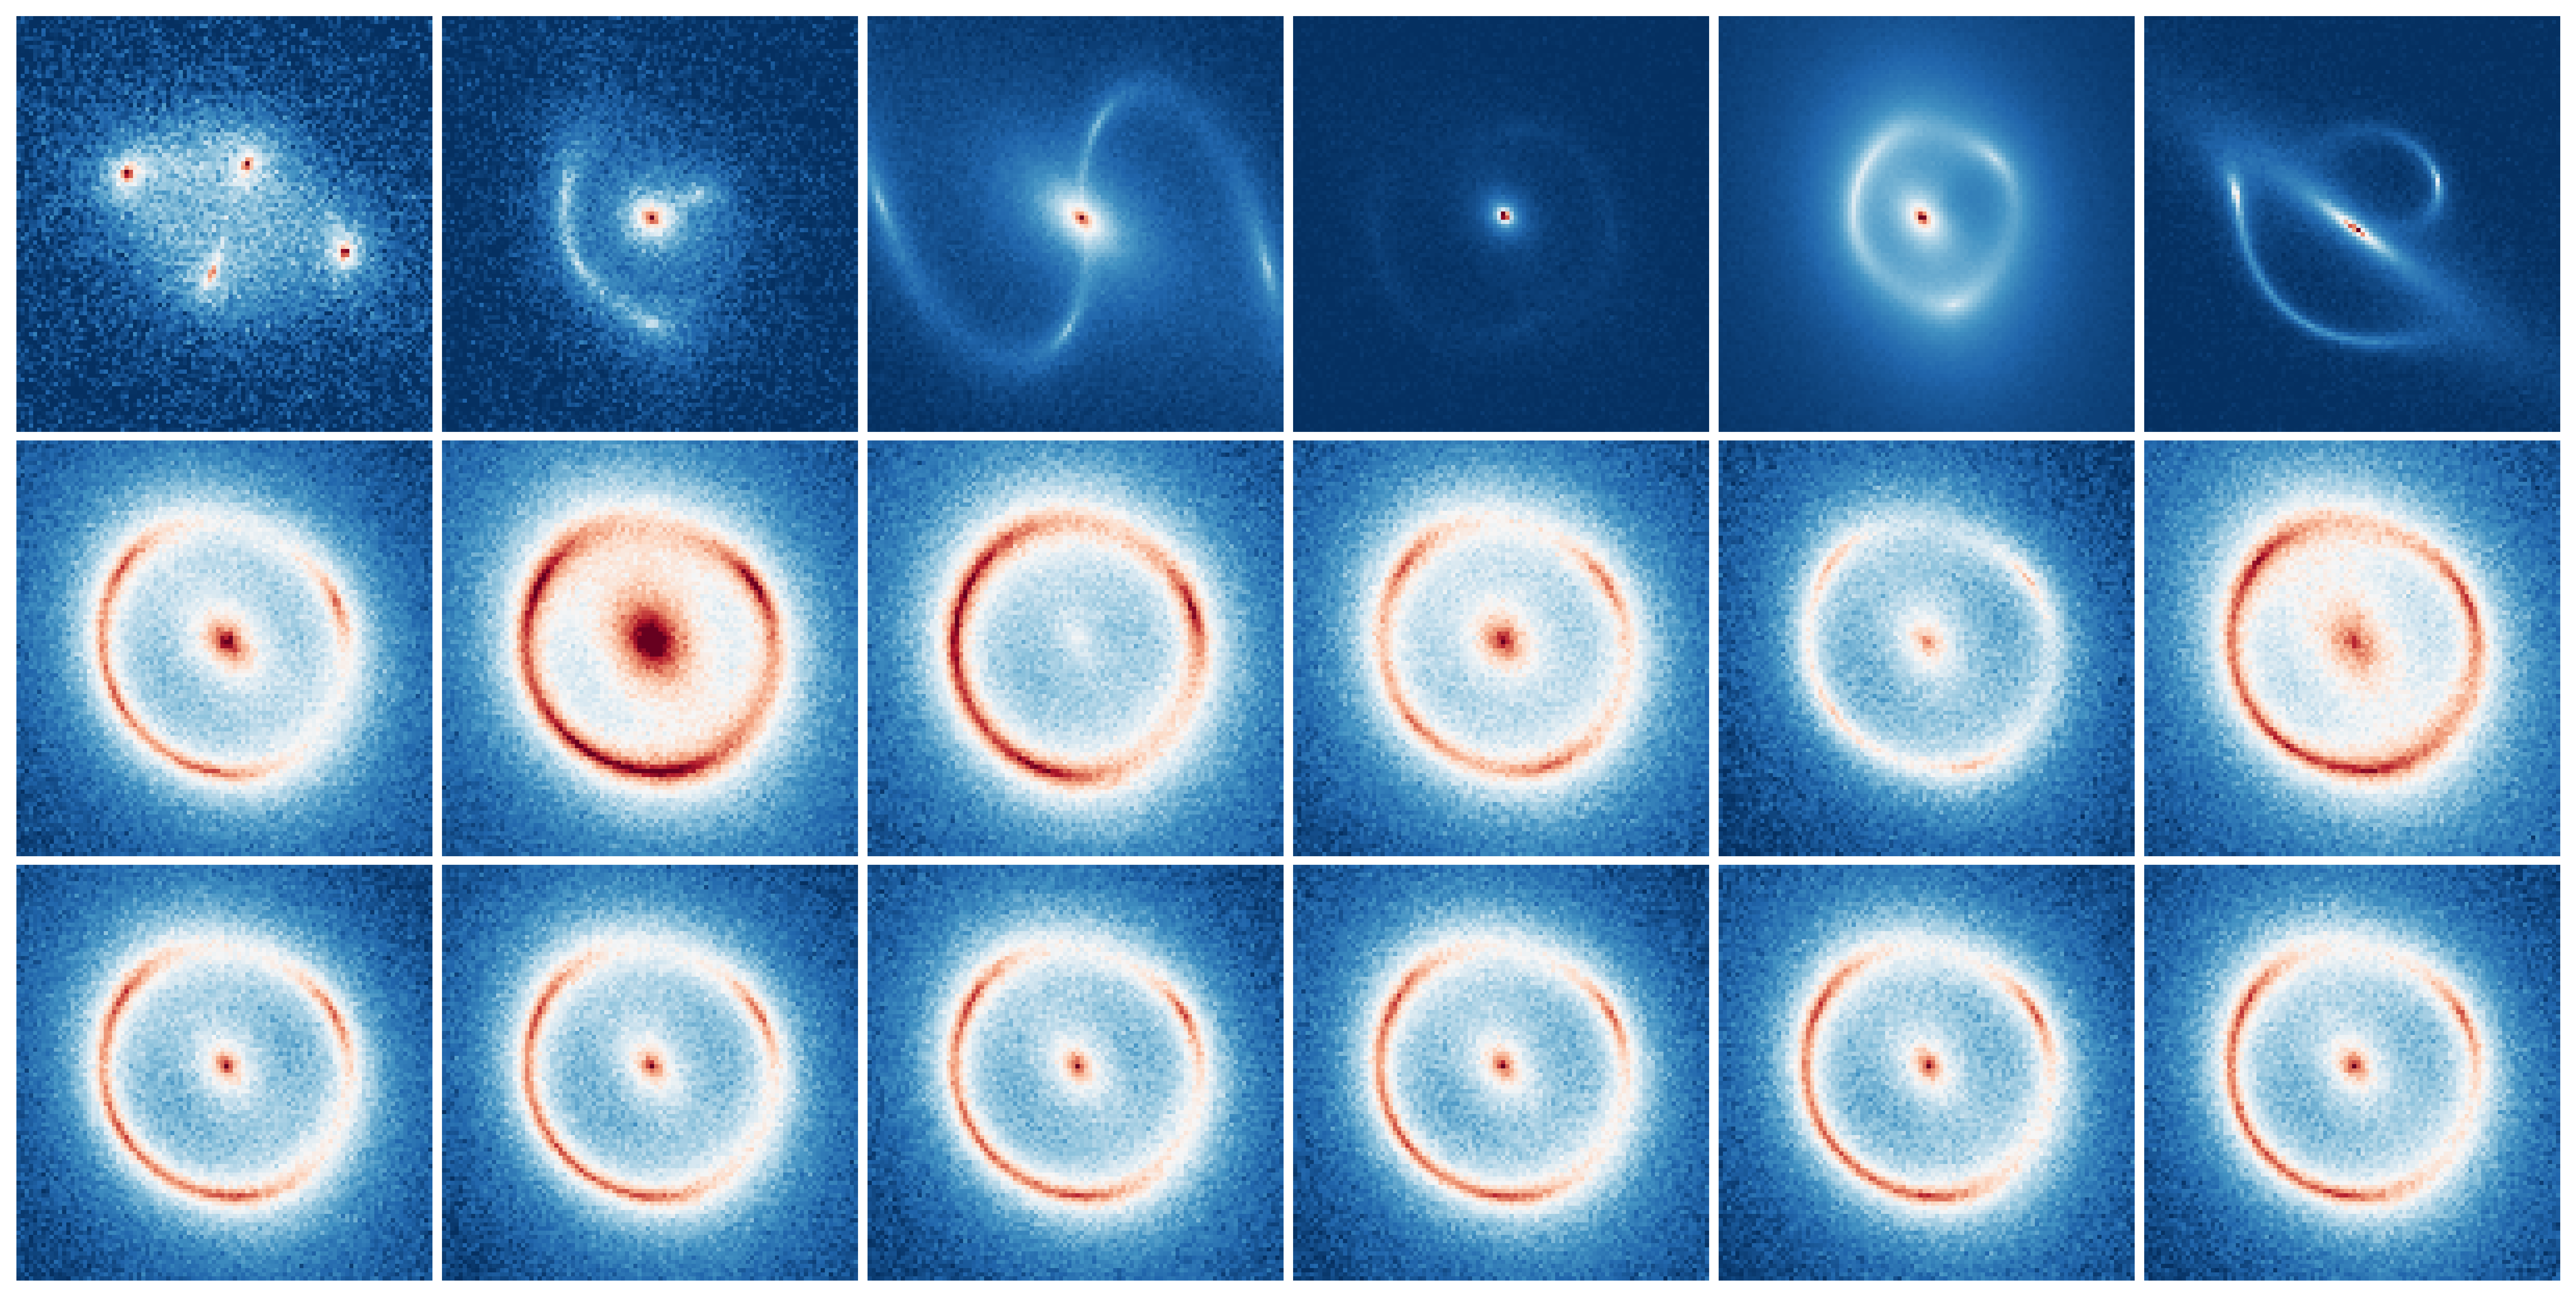
\includegraphics[width=0.7\linewidth]{ANRE-targeted.png}};
  \node[left=of img, node distance=0.5cm, text width=1cm, yshift=+1.5cm, anchor=center] {Full prior};
  \node[left=of img, node distance=0.5cm, text width=1cm, anchor=center] {Box\\ truncation};
  \node[left=of img, node distance=0.5cm, text width=1cm, yshift=-1.5cm, anchor=center] {Correlated\\ truncation};
 \end{tikzpicture}
\caption{Targeted training data. The simulations in the first row are drawn from the full initial prior, described in Table~\ref{tab:anre-lensing-params}. In the intermediate row, we show simulations used for the last round of training of the 1-dimensional marginal ratio estimators, where the macro-model parameters were drawn from the most constrained hyper-rectangular box prior. In the last row, the macro-model parameters were sampled from the high-dimensional constrained prior with the slice-based nested sampler. The images in the second and last row are plotted in the same color scale, whereas the ones in the first row are allowed to vary for visualization purposes since they exhibit a larger variance.
}
\label{fig:targeted_data}
\end{figure}

Having reduced the macro-model parameters training data variance, we are then able to focus on substructure parameter inference, for which the results are shown in Figure~\ref{fig:corner}. These results were obtained with two sequential rounds of inference using a correlated truncation scheme, as first explained in Section~\ref{subsec:tmnre-t}. In contrast, given the initial fixed simulation budget, we were not able to constrain the subhalo parameter in our target observation with the data variance displayed by simulations using only box truncation. 


\section{Discussion and conclusions} \label{sec:anre-conclusion}

 The motivation for the \gls*{sbi} method development presented in this work comes from the data analysis and statistics challenges facing the fields of astrophysics and cosmology in light of high quality data from current and future experiments \cite{EUCLID:2011zbd, Gardner:2006ky,LSSTDarkEnergyScience:2012kar, Neichel:2018aa, Prusti:2016aa, Lazio:2009aa, Knodlseder:2020onx}. In this work, we have focused on one specific \gls*{sbi} algorithm, \gls*{tmnre}, and advanced its potential with the introduction of two new components:
\begin{enumerate}[a)]
    \item \emph{Autoregressive \gls*{nre}}, presented in Section~\ref{subsec:anre-anre}, estimates multi-dimensional (marginal) posteriors by effectively computing $d$ 1-dimensional conditional ratios instead of a $d$-dimensional joint one (see Equation~\eqref{eq:anre-autoregressive}). This way of approaching high-dimensional distribution estimation through an autoregressive scheme has been motivated by its proven scaling potential in other \gls*{sbi} techniques \cite{Germain:2015yft, Uria:2016aa, Papamakarios:2017tec}. We release a publicly available implementation of the autoregressive model in the \gls*{tmnre} package \texttt{swyft}\footnote{\url{https://github.com/undark-lab/swyft}}.
    \item Our \emph{slice-based nested sampling} implementation, presented in Section~\ref{subsec:anre-ns}, offers vectorized evaluations of the natively GPU-based ratio estimator and introduces a convergence criterion related to posterior mass. The latter is essential for sequential inference applications since it allows one to define the truncation region in Equation~\eqref{eq:gamma_r}. The sampler choice naturally comes from the realisation that nested sampling techniques provide a tool to efficiently sample not only from a multi-dimensional posterior, but also natively from a constrained prior. Our slice sampler implementation is available in the package \texttt{torchns}\footnote{\url{https://github.com/undark-lab/torchns}}.
\end{enumerate}
We have demonstrated their application in three case studies presented in Section~\ref{sec:anre-experiments}. Firstly, we tested the performance of the autoregressive ratio model against the non-autoregressive one in a toy example. The main results, for different simulation budgets and dimensionality, are presented in Figure~\ref{fig:toy}. Secondly, we explored how variable ordering impacts the autoregressive model in a stellar streams analysis. We have found that a non-optimal variable ordering does have an impact, but does not severely penalise the overall inference result in our specific application, as shown in Figure~\ref{fig:streams_loss}. Lastly, we investigated the potential of a correlated truncation scheme in a proof-of-concept application to substructure searches in a strong gravitational lensing image. The main outcomes are exhibited in Figs.~\ref{fig:corner} and~\ref{fig:targeted_data}: in particular, given our fixed simulation budget, the non-autoregressive model is not able to estimate the macro-model parameter joint distribution, and only through correlated prior truncation are we able to constrain the subhalo parameters.

\vspace{10pt}
 \emph{Outlook.} There are two aspects to consider as far as outlook is concerned for our method development. The first concerns the known limitations of the autoregressive modeling and the nested sampling techniques. The second is more general, and considers the analysis settings in which this approach may be useful.

As discussed above, one of the potential limitations of autoregressive modeling is its sensitivity to parameter orderings. Although we investigated this in the context of stellar streams in Section~\ref{subsec:anre-stream}, and found that the effect was minimal, it is possible that this is model dependent. As such, to extend the method, it would be interesting to develop techniques to derive an (approximately) optimal ordering of the parameters, \eg~by estimating the strength of correlations between various parameter sets. 

On the nested sampling side, known limitations include the fact that it becomes very costly in terms of the required number of network evaluations for high dimensional parameter spaces, say $d \gtrsim 30$ (for a discussion see, \eg, Ref.~\cite{Buchner:2021kpm}). As such, it will be interesting to further investigate methods that exploit gradient information and scale better to high dimensions, such as the proximal nested sampling technique proposed in Ref.~\cite{Cai:2002aa}. Moreover, our current implementation of the slice sampler does not include clustering detectors (see \eg~Ref.~\cite{Feroz:2007kg}), which makes it inefficient for multi-modal posteriors.

More generally, we believe the method we have developed could be useful in the following type of scenario: suppose that a part of the parameter space dominates the data variance, but is not the one that we are ultimately most interested in performing inference on. Using traditional methods, there are typically two approaches: a) solve the full joint analysis problem for all parameters, but face significant computational challenges, or b) analyse the nuisance parameters separately, and then fix them to some form of best-fit value to use in the rest of the analysis, at the cost of neglecting their uncertainties. For example, as briefly mentioned in Section~\ref{subsec:lensing}, this is exactly the scenario in standard strong gravitational lensing analyses where the lens light gets subtracted assuming the best-fit value, before analysing the lensed emission.

With the method developed in this work, however, there is an alternative approach available. In particular, as explained in Section~\ref{subsec:tmnre-t}, the fact that prior truncation composes well with marginalisation allows us to consistently combine different analysis strategies that target distinct parts, or ``blocks", of the model into a coherent ``inference assembly". This exact procedure was exemplified in Section~\ref{subsec:lensing}, where we first reduced training data variance by truncating the lens and lensed source parameters, and then performed sequential inference on our parameters of interest, the ones pertaining the substructure.

In conclusion, this approach can be relevant for many different cosmological and astrophysical applications, where the analysis would be carried out simultaneously on different components of the systems, \eg~parameters of interest, foregrounds, backgrounds, nuisance parameters, instrumentation parameters \textit{etc}. Ultimately, this will allow us to flexibly combine different inference strategies in order to draw coherent and consistent conclusions based on the full model and all the data.

%\section*{Acknowledgements}
%
%We thank Will Handley and Kilian Scheutwinkel for useful discussions. This work is part of a project that has received funding from the European Research Council (ERC) under the European Union’s Horizon 2020 research and innovation program (Grant agreement No. 864035 -- UnDark). JA is supported through the research program ``The Hidden Universe of Weakly Interacting Particles" with project number 680.92.18.03 (NWO Vrije Programma), which is partly financed by the Nederlandse Organisatie voor Wetenschappelijk Onderzoek (Dutch Research Council). 
%This work was carried out on the Snellius Compute Cluster at SURFsara. We acknowledge the use of the \texttt{python} \cite{python} modules, \texttt{matplotlib} \cite{Hunter:2007ouj}, \texttt{numpy} \cite{Harris:2020xlr},  \texttt{scipy} \cite{Virtanen:2019joe}, \texttt{AstroPy} \cite{Astropy:2013muo}, \texttt{PyTorch} \cite{pytorch}, \texttt{tqdm} \cite{tqdm}, and \texttt{jupyter} \cite{jupyter}.


%%%%%%%%%%%%%%%%% APPENDICES %%%%%%%%%%%%%%%%%%%%%

\begin{subappendices}

\section{Another formulation} \label{apx:anre-anre}

 The autoregressive model presented in Section~\ref{subsec:anre-anre} can be also written with a single network that can estimate both components. In order to do this, we introduce an auxiliary variable $c = -1, 1$.  We then consider the ratio
\begin{equation}
    r(\theta_i; \data, c, \interest_{1:i-1})
    =\frac
    {
    p'(\theta_i \mid \data, c, \interest_{1:i-1})
    }{
    p(\theta_i)
    %\mid \data, c, \interest_{1:i-1})
    }
\end{equation}
The distribution of our auxiliary model is now given by
\begin{equation}
	\theta_i, \data, c, \interest_{1:i-1} \sim p'(\data , c, \theta_i, \interest_{1:i-1})\equiv p'(\data \mid c, \theta_i, \interest_{1:i-1})p(c) p(\interest_{1:i})\;,
\end{equation}
where we make use of the definitions
$p'(\data \mid c = -1, \theta_i, \interest_{1:i-1}) \equiv p(\data)$  and
$p'(\data \mid c = 1, \theta_i, \interest_{1:i-1}) \equiv
p(\data \mid \theta_i, \interest_{1:i-1})$.

Once the above ratio estimator is trained, we can obtain the desired conditional posterior-to-conditional prior ratio by using
\begin{equation}
\frac{
p(\theta_i \mid \data, \interest_{1:i-1})
}{
p(\theta_i \mid \interest_{1:i-1})
}
\approx
\frac{
r(\theta_i ; \data, c = +1, \interest_{1:i-1})
}{
r(\theta_i ; \data, c = -1, \interest_{1:i-1})
}\;.
\end{equation}

The advantage of this formulation is that it reduces the number of networks to train by a factor of two, which should correspondingly reduce GPU memory requirements and training time. A potential downside of this approach is that the network capacity has to be high enough in order to efficiently learn both posterior and prior approximations at the same time. We will leave a quantitative comparison between different methods and network architectures to future work.


\section{Multivariate Gaussian experiment}
\label{apx:anre-toy}
 In Figure~\ref{fig:toy_corner}, we show the agreement between the analytical and estimated posteriors for the \gls*{nre} and ANRE methods applied to the toy problem described in \autoref{toy}. We see that across all $10$ parameters the autoregressive model achieves almost perfect agreement with the analytic result.

In order to check the impact of the autoregressive ordering in this Multivariate Gaussian toy example we have conducted an additional test for $10$ dimensions. For this test, we use a likelihood with fixed covariance $\mathbf{\Sigma}$, which has correlation scales of $0.1$ for the off-diagonal entries, and varying diagonal correlation scales, ranging from $0.1$ to $0.55$ in $0.05$ steps. We have run our autoregressive model for four different variable orderings: from most constrained to least, from least constrained to most, and two random orderings. The results shown in Figure~\ref{fig:toy_ordering} demonstrate that the autoregressive ordering does not have an impact in this case.

\begin{table}
    \centering
    \renewcommand{\arraystretch}{1.2}
    \begin{tabular}{l c c c c r}
        \hline
        Parameter & True value & Initial prior  \\
        \hline
        $t_\mathrm{age}\,\mathrm{[Myr]}$ & 3000 & $\mathcal{U}(2583, 3647)$ \\
        $\lambda_\mathrm{rel}$ & 1.405 & $\mathcal{U}(0.13, 2.00)$ \\
        $\lambda_\mathrm{match}$ & 1.846 & $\mathcal{U}(0.31, 2.00)$ \\
        $\xi_0$ & 0.001 & $\mathcal{U}(0.0001,0.01)$ \\
        $\alpha$ & 20.9 & $\mathcal{U}(10.0, 30.0)$ \\
        $r_h \, \mathrm{[pc]}$ & 0.001 & $\mathcal{U}(0.0001, 0.01)$ \\
        $\bar{m}\,\mathrm{[M}_\odot\mathrm{]}$ & 3 & $\mathcal{U}(1.0, 20.0)$ \\
        $\log(M_\mathrm{sat}/\mathrm{M}_\odot)$ & 4.05 & $\mathcal{U}(3.3, 4.5)$ \\
        $\sigma_v \,\mathrm{[km/s]}$ & 1.1 & $\mathcal{U}(0.96, 1.32)$ \\
        $x_c\,\mathrm{[kpc]}$ & 11.8 & $\mathcal{U}(117, 119)$ \\
        $y_c\,\mathrm{[kpc]}$ & 0.79 & $\mathcal{U}(0.6, 1.1)$ \\
        $z_c\,\mathrm{[kpc]}$ & 6.4 & $\mathcal{U}(6.32, 6.54)$ \\
        $v_{x,c}\,\mathrm{[km/s]}$ & 109.5 & $\mathcal{U}(106.8, 113.7)$ \\
        $v_{y,c}\,\mathrm{[km/s]}$ & -254.5 & $\mathcal{U}(-256, -251)$ \\
        $v_{z,c}\,\mathrm{[km/s]}$ & -90.3 & $\mathcal{U}(-93.3,-84.6)$ \\
        $p_\mathrm{near}$ & 0.5 & $\mathcal{U}(0.34, 0.72)$ \\
        \hline
    \end{tabular}
    \caption{True parameter values and priors used in the \gls*{tmnre} inference round for the stellar streams example. Note that our prior choices are taken from the final round of inference of Ref.~\protect\cite{Alvey:2023pkx} so as to test the autoregressive model in a final round of precision inference through active learning.}
    \label{tab:anre-streams-params}
\end{table}

\begin{figure*}
\centering
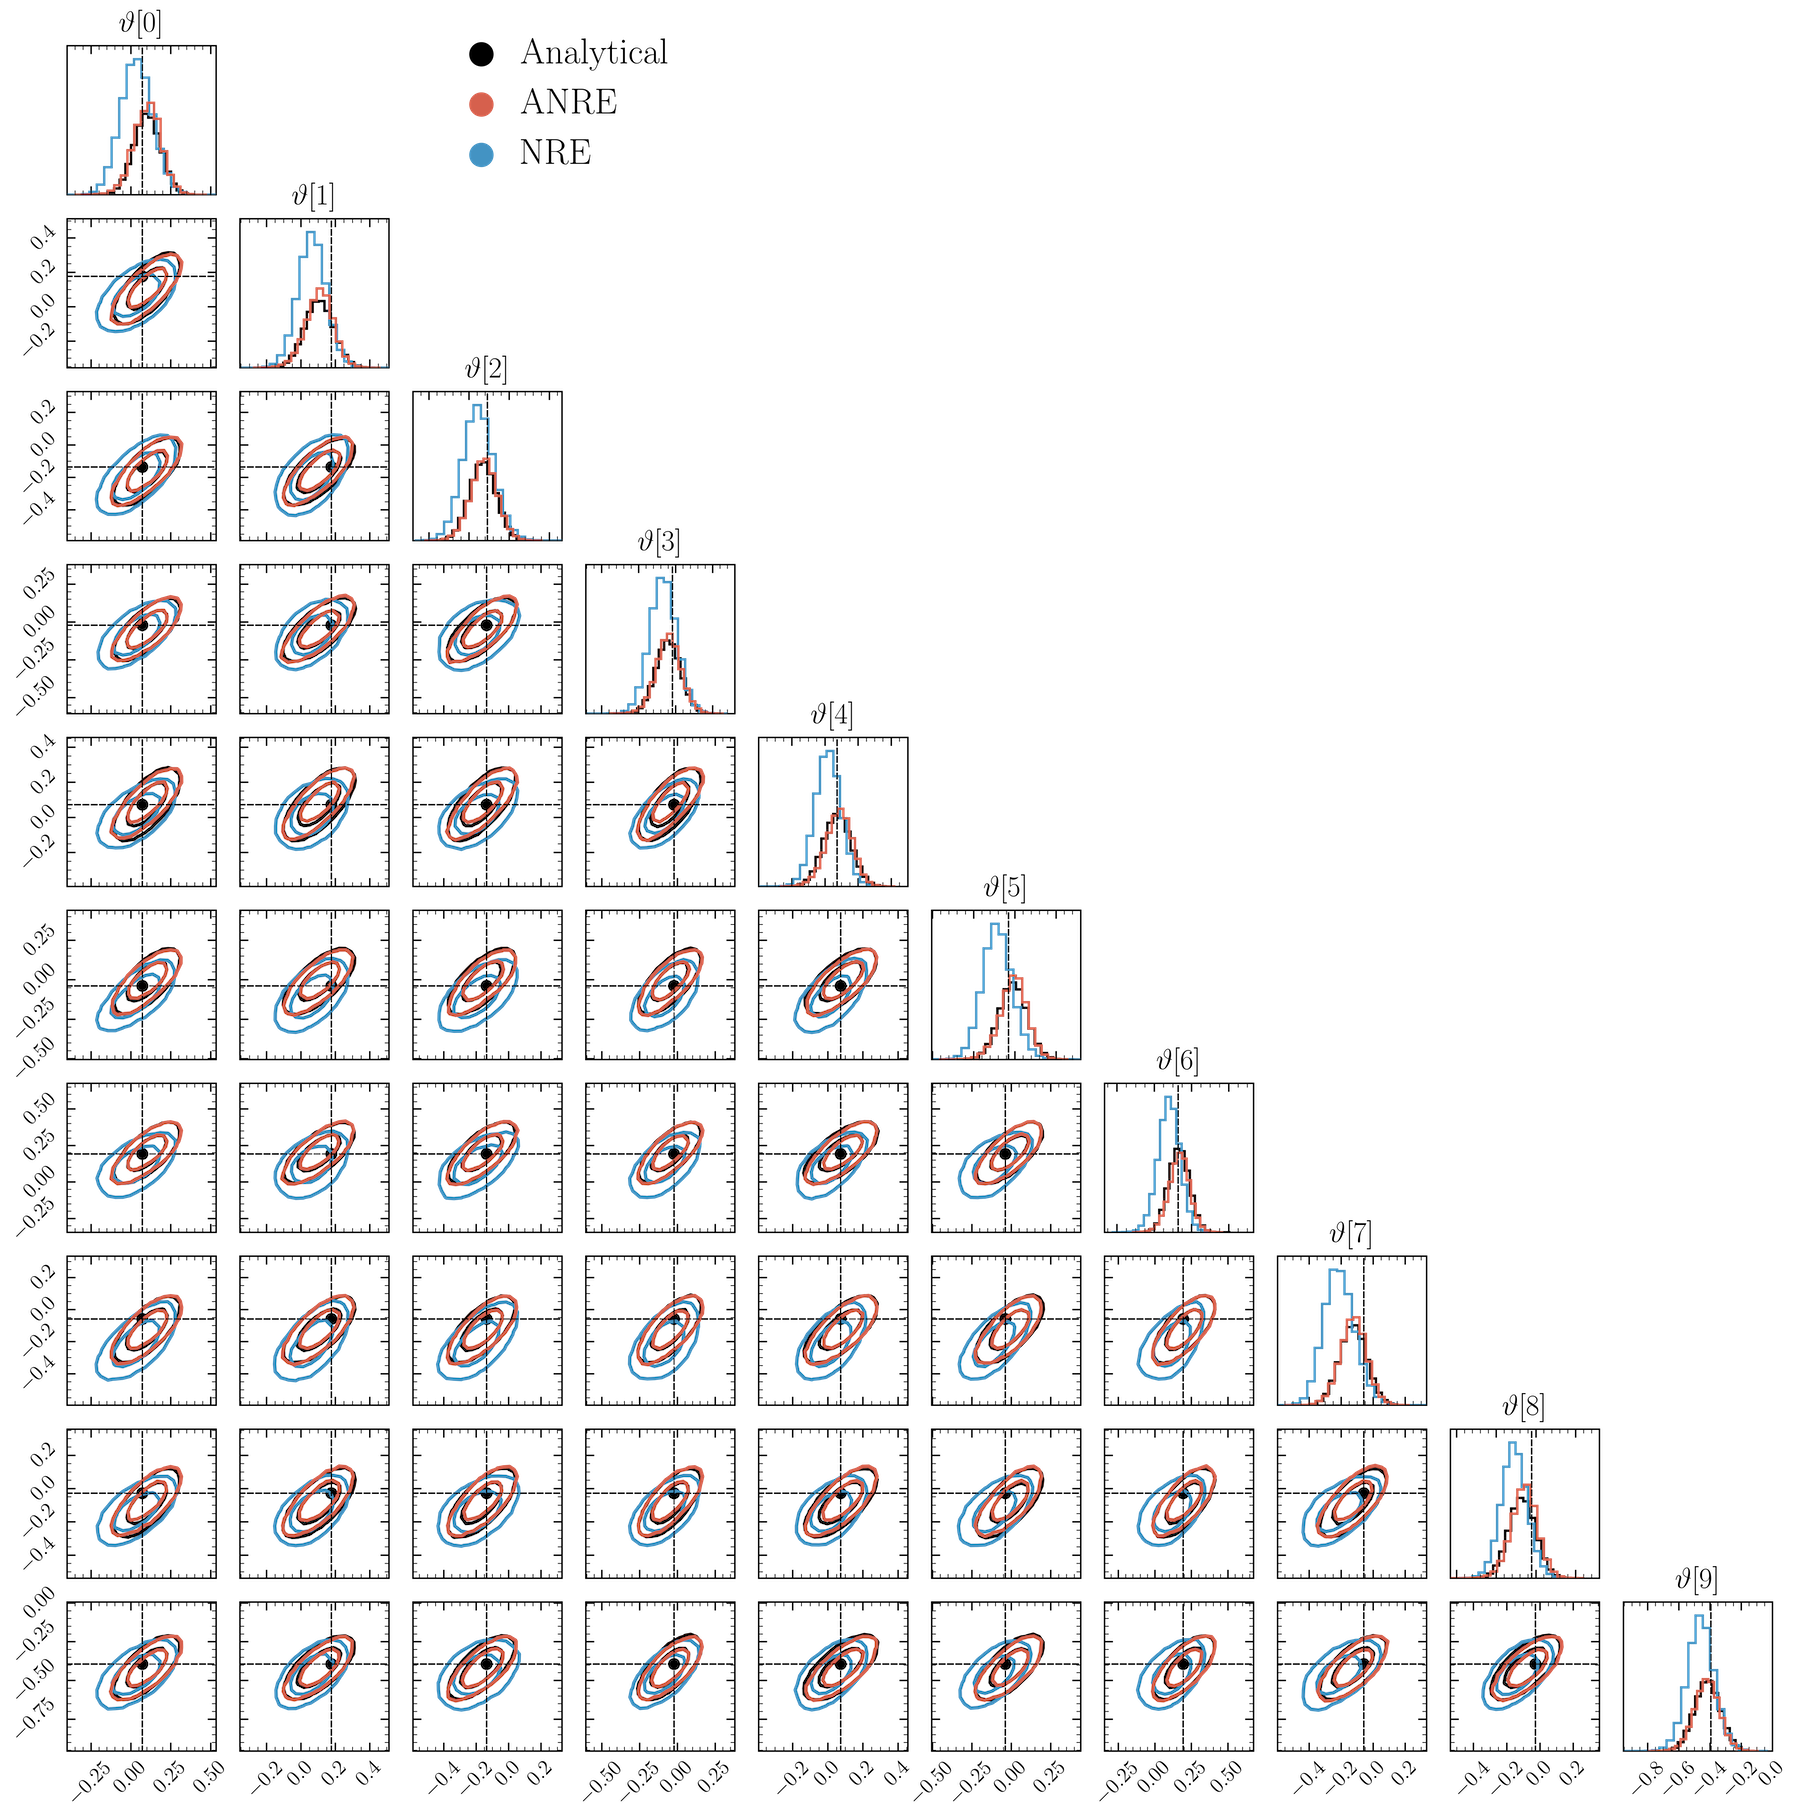
\includegraphics[width=\linewidth]{ANRE-toy_corner.png}
\caption{
 Multivariate Gaussian toy example results. Corner plot highlighting the agreement between the analytic and estimated posteriors for the $d = 10$ Gaussian model described in \autoref{toy}.}
\label{fig:toy_corner}
\end{figure*}

\begin{figure*}
\centering
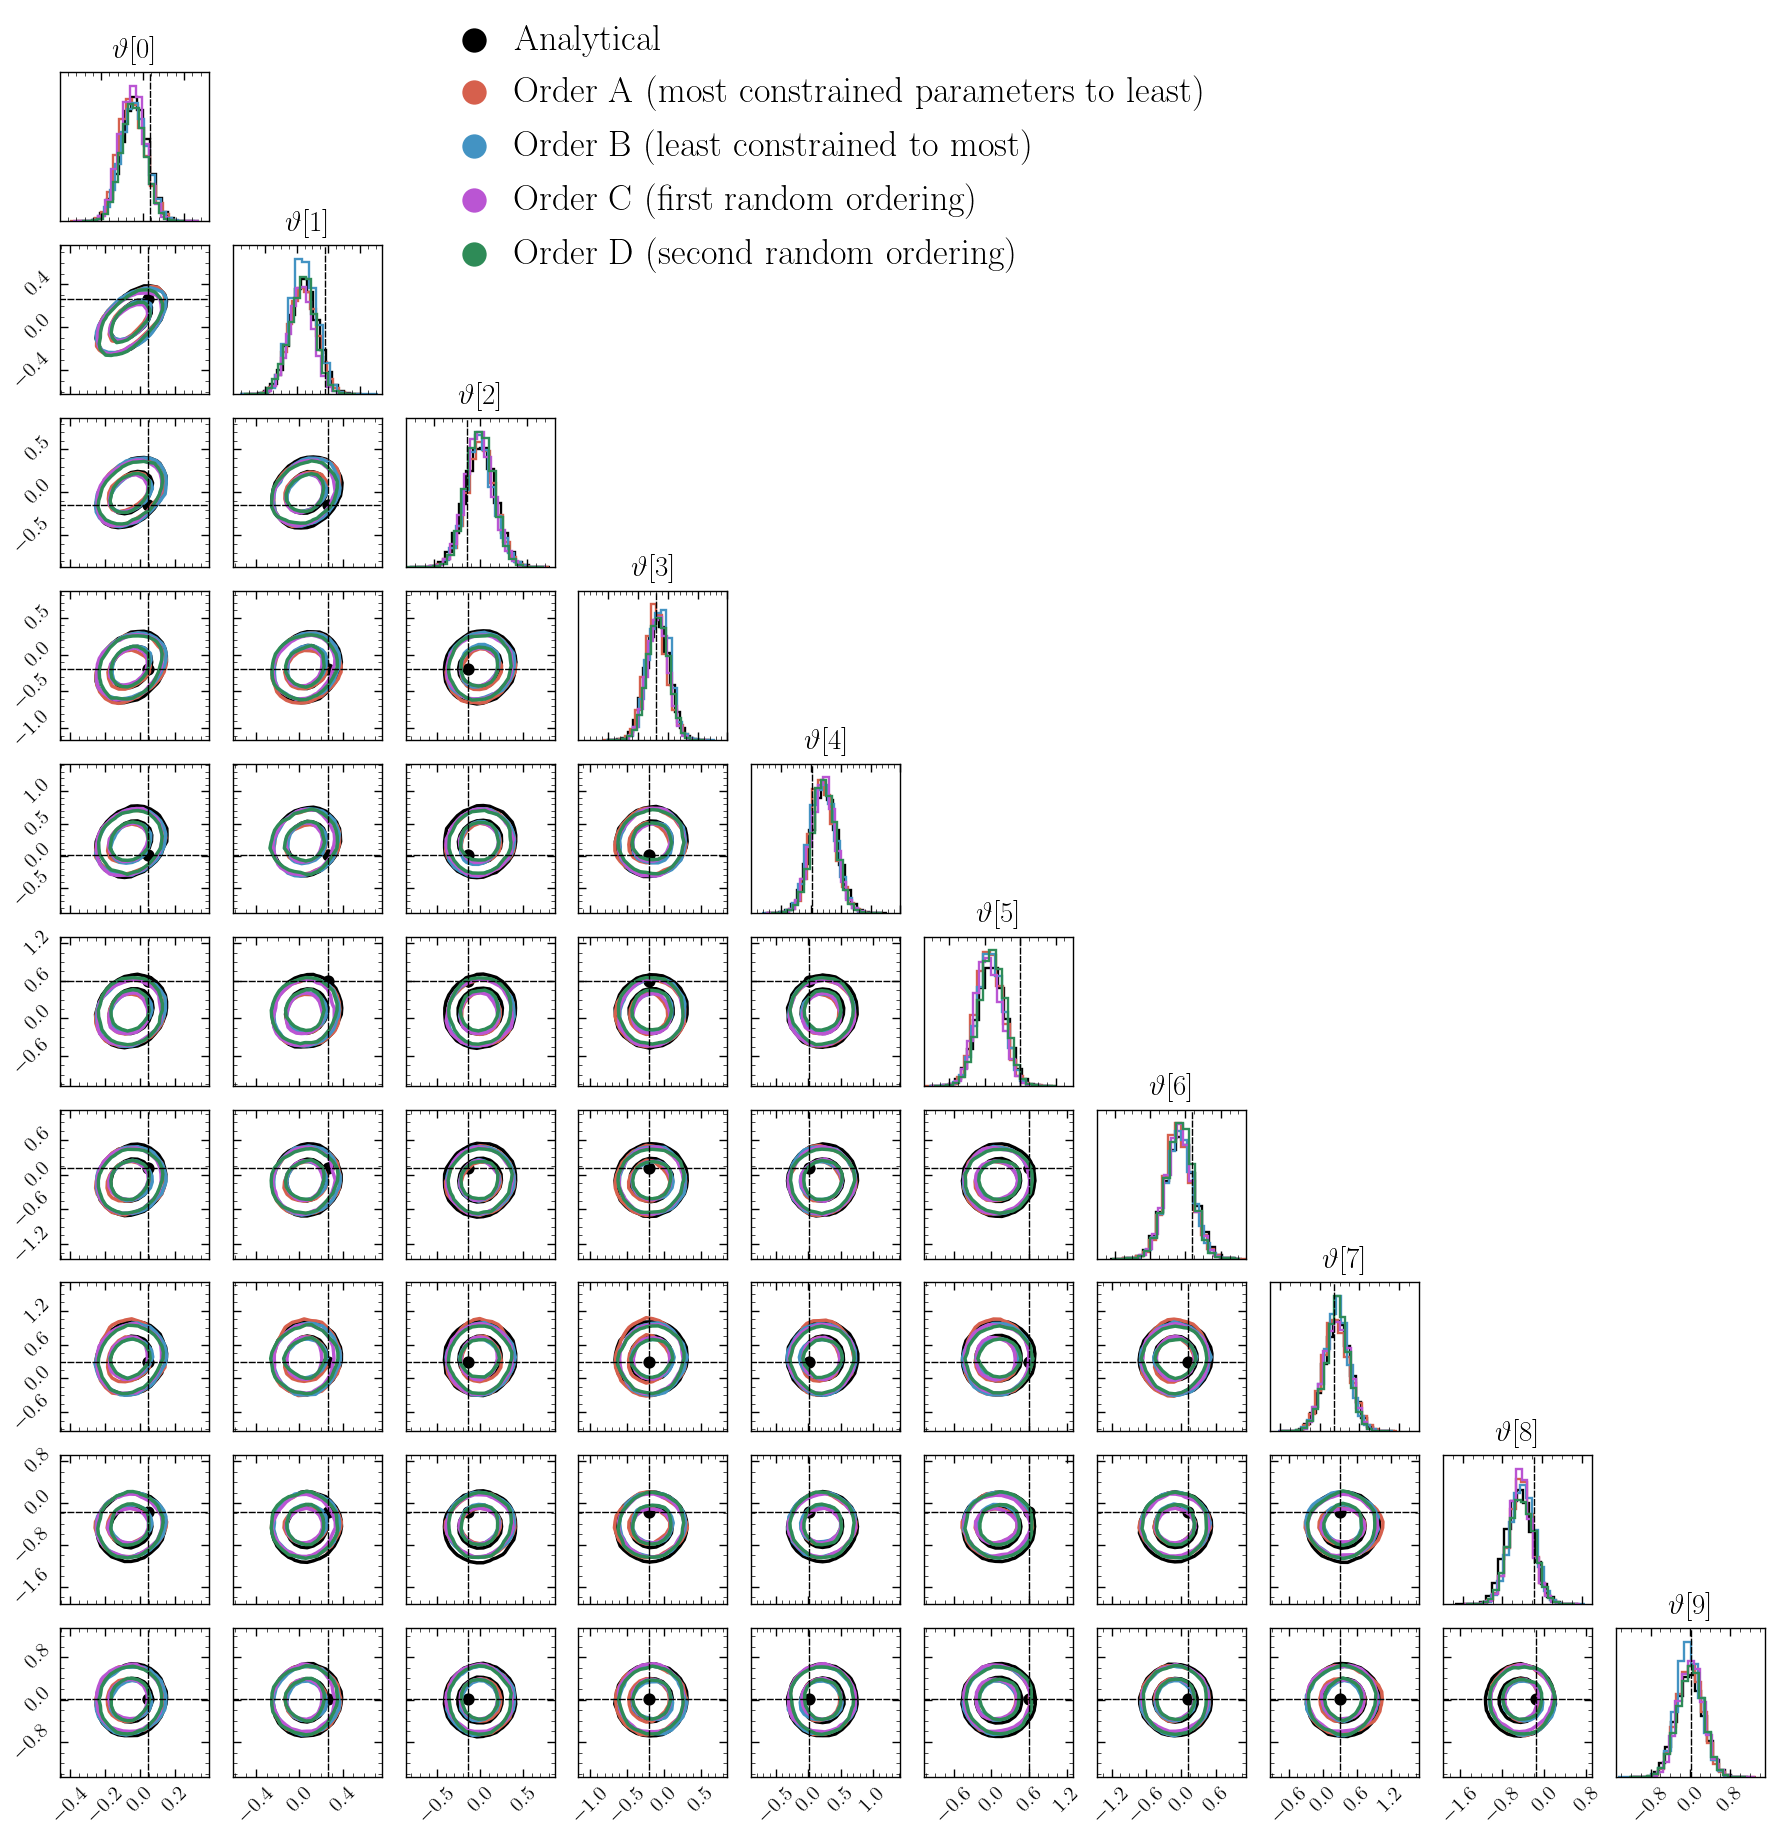
\includegraphics[width=\linewidth]{ANRE-toy_ordering.png}
\caption{
 Multivariate Gaussian toy example results. Corner plot highlighting the agreement between the analytic and estimated posteriors for the $d = 10$ Gaussian model described in \autoref{toy} and Appendix~\ref{apx:anre-toy}. For the estimated posteriors we have used four different orderings, as described in Appendix~\ref{apx:anre-toy}.}
\label{fig:toy_ordering}
\end{figure*}

\section{Stellar streams experiment}
\label{apx:anre-streams}

 In this short appendix we present the technical details relevant for the stellar streams experiment presented in Section~\ref{subsec:anre-stream}. There are a number of things directly analogous to the implementation described in Ref.~\cite{Alvey:2023pkx}. In particular, we use the stellar streams simulator, \texttt{sstrax} \cite{sstrax}, developed in this reference, as well as the \texttt{swyft}-based inference code \texttt{albatross} \cite{albatross}. In addition, we consider the same set of model parameters (described in Table~\ref{tab:anre-streams-params} and in detail in Ref.~\cite{Alvey:2023pkx}), the same injection parameters to generate the observation, and the same binning/observation scheme. The key difference with respect to this reference is in the inference network used. In particular, we replace the $1$-dimensional ratio estimation across all model parameters with the autoregressive method described in this work to model their joint distribution. In terms of network training details, we use the Adam optimiser with an initial learning rate of $10^{-6}$. In addition, we use a batch size of $512$ and a simulation budget of $3\times 10^5$ training examples. Finally, we use the following orderings (Order A and Order B referenced in the main text) for training the autoregressive ratio estimator: [$\sigma_v$, $x_c$, $y_c$, $z_c$, $v_{x,c}$, $v_{y, c}$, $v_{z, c}$, $t_\mathrm{age}$, $p_\mathrm{near}$, $\lambda_\mathrm{rel}$, $\lambda_{match}$, $\xi_0$, $\alpha$, $r_h$, $\bar{m}$, $\log(M_\mathrm{sat}/\mathrm{M}_\odot)$] (Order A), and [$\xi_0$, $\lambda_{match}$, $\lambda_\mathrm{rel}$, $\alpha$, $r_h$, $\bar{m}$, $\log(M_\mathrm{sat}/\mathrm{M}_\odot)$, $t_\mathrm{age}$, $\sigma_v$, $x_c$, $y_c$, $z_c$, $v_{x,c}$, $v_{y, c}$, $v_{z, c}$, $p_\mathrm{near}$] (Order B).

In Figure~\ref{fig:corner_streams_2}, we also show the results of a test with two additional random orderings. Specifically, the orderings shown are [$\alpha$, $\log(M_\mathrm{sat}/\mathrm{M}_\odot)$, $\lambda_\mathrm{rel}$, $\xi_0$, $v_{x,c}$, $\sigma_v$, $v_{z,c}$, $\bar{m}$, $t_\mathrm{age}$, $r_h$, $x_c$, $z_c$, $p_\mathrm{near}$, $\lambda_\mathrm{match}$, $y_c$, $v_{y,c}$] (first random order) and [$v_{z,c}$, $p_\mathrm{near}$, $\bar{m}$, $\sigma_v$, $v_{y,c}$, $\alpha$, $v_{x, c}$, $t_\mathrm{age}$, $\lambda_{\mathrm{rel}}$, $z_c$, $\lambda_\mathrm{match}$, $y_c$, $x_c$, $\xi_0$, $r_h$, $\log(M_\mathrm{sat}/\mathrm{M}_\odot)$] (second random order).

Furthermore, we performed an additional test in order to check when the loss for order B reaches the one for order A in Figure~\ref{fig:streams_loss} (see main text for definitions), by gradually increasing the simulation budget.
Figure~\ref{fig:anre-training} shows the loss for order B as a function of epochs, for different sizes of training dataset, with the biggest one (100\% in the figure) containing $6\times10^5$ simulations. From Figure~\ref{fig:anre-training}, we can see that the loss for order B reaches a plateau value of -6.1 (the one of the loss for order A in Figure~\ref{fig:streams_loss} when training on $3\times10^5$ simulations) for approximately between 60\% to 70\% of the total $6\times10^5$ simulations, so roughly for $4\times10^5$ simulations. In this specific example, this experimental check shows that a network trained with order B needs 25\% more simulations to plateau at the same loss as one trained for order A. This test further confirms our observation that the ‘penalty’ for choosing a non-optimal ordering is not severe, and can be easily circumvented, for example as in this case, by increasing the simulation budget. However, the important take away message is that the simulation computational budget can be reduced by choosing an optimal ordering. 

\begin{figure*}
    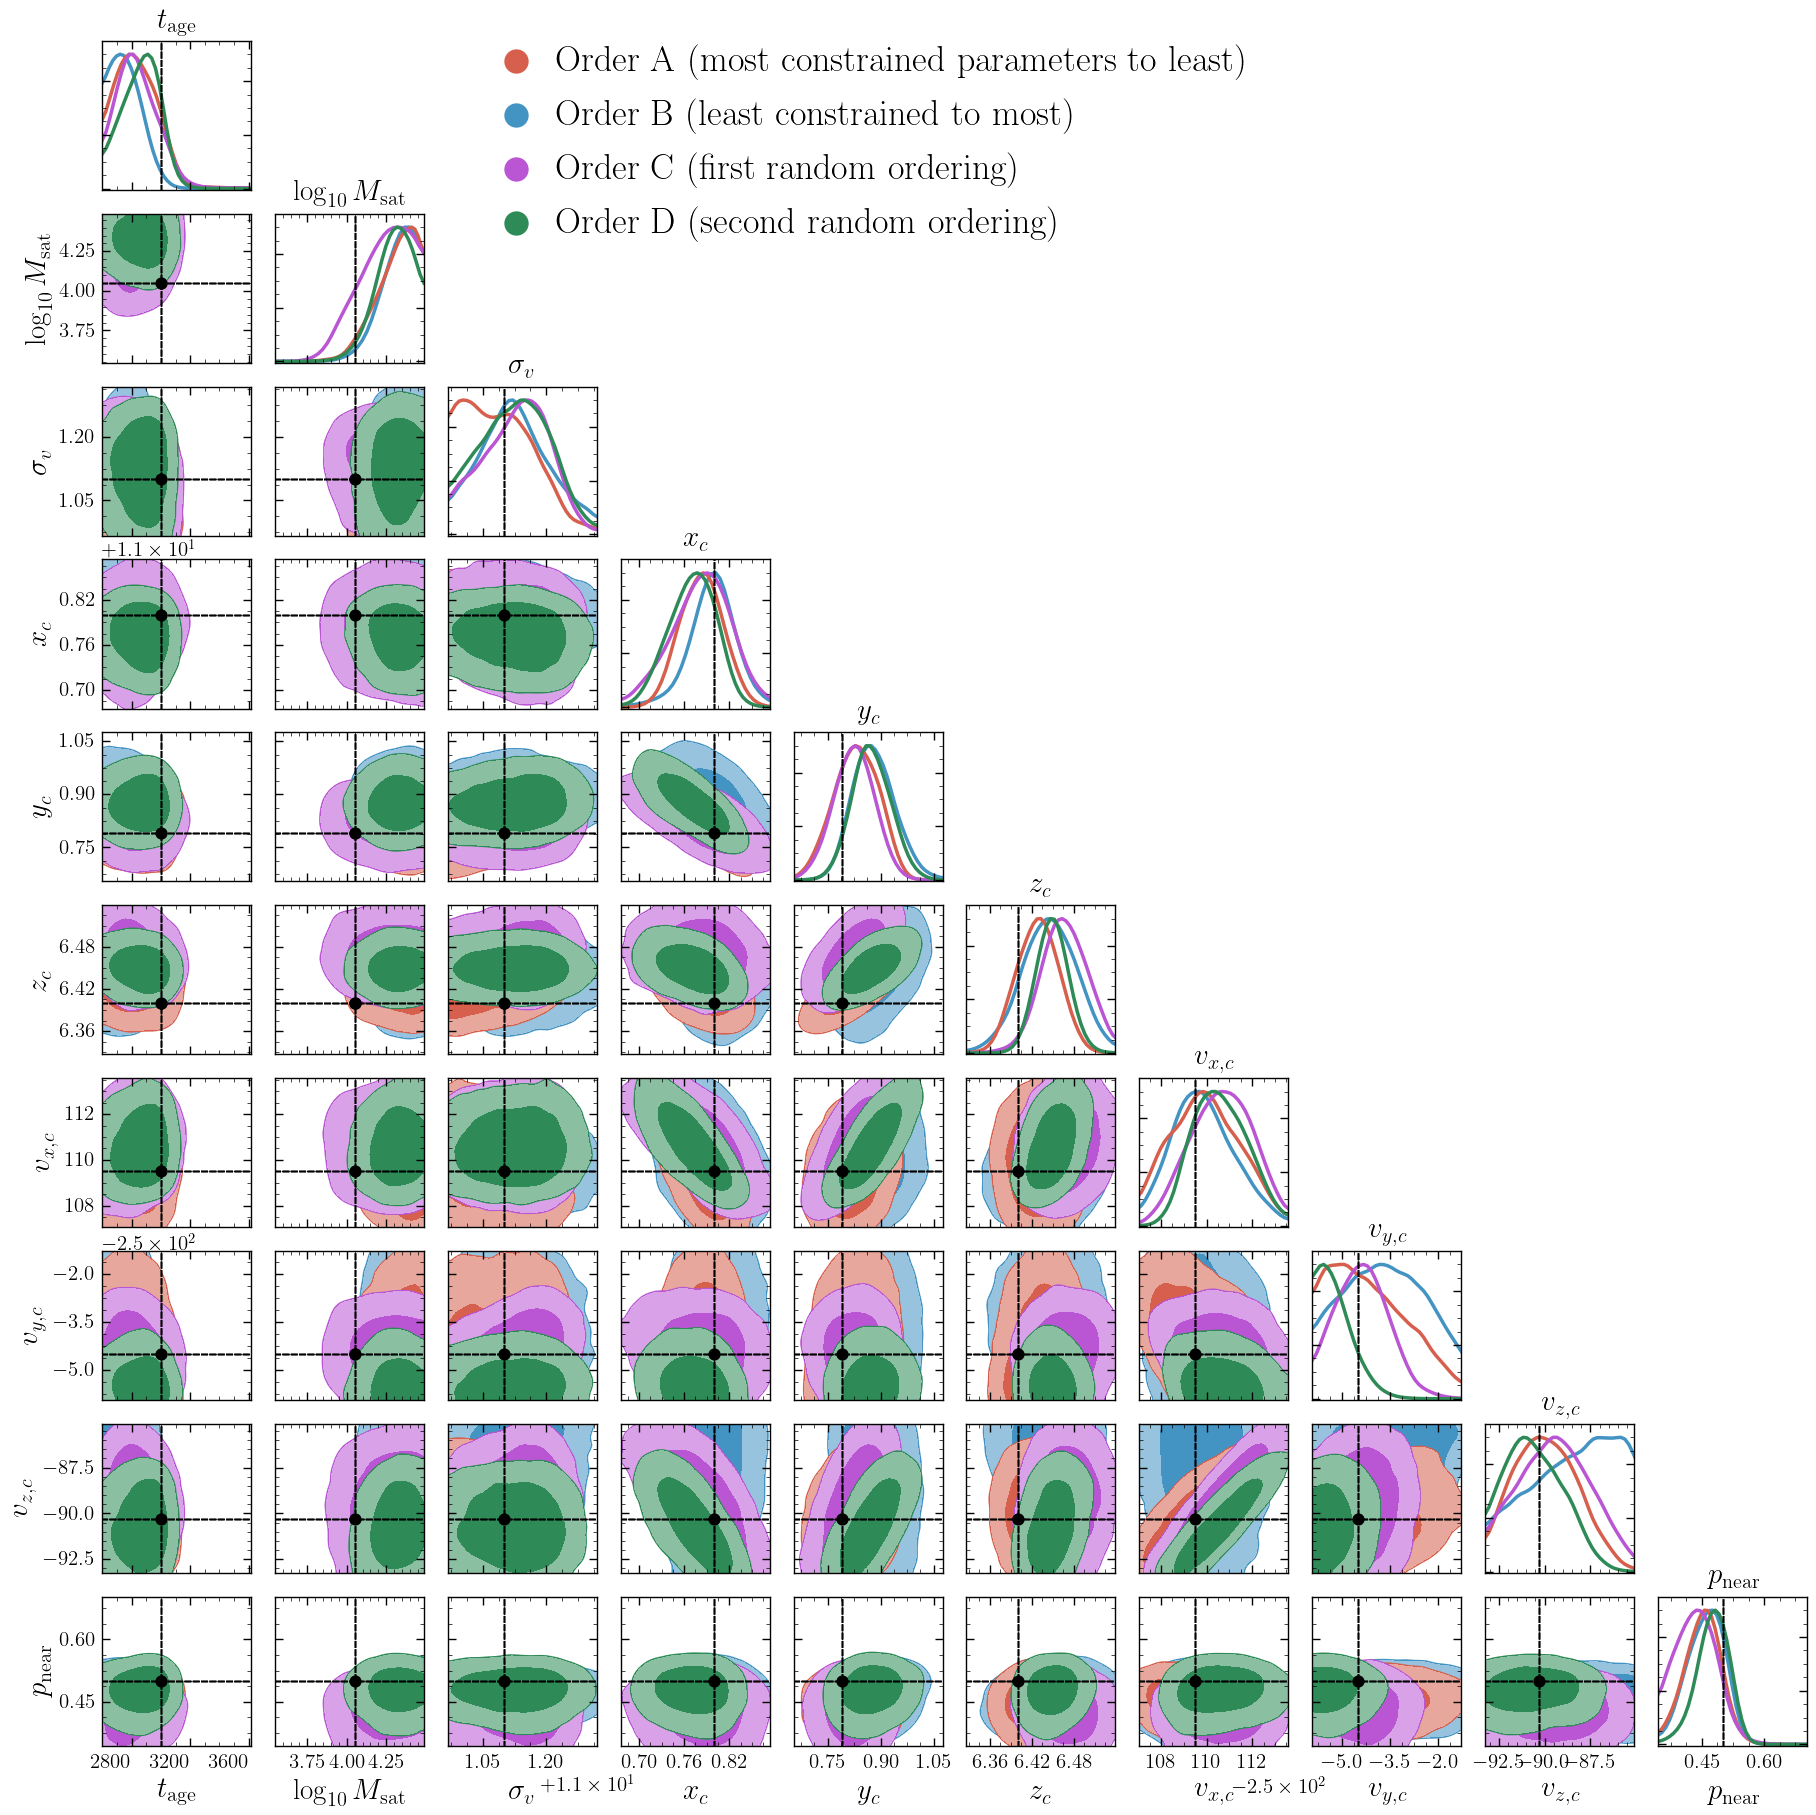
\includegraphics[width=\linewidth]{ANRE-corner_streams_2.png}
    \caption{Additional checks of the variable ordering conclusions given in Section~\ref{subsec:anre-stream}. Here, we overlay the results presented in the main text with inference results given two other random orderings.}
    \label{fig:corner_streams_2}
\end{figure*}

\begin{figure}
    \centering
    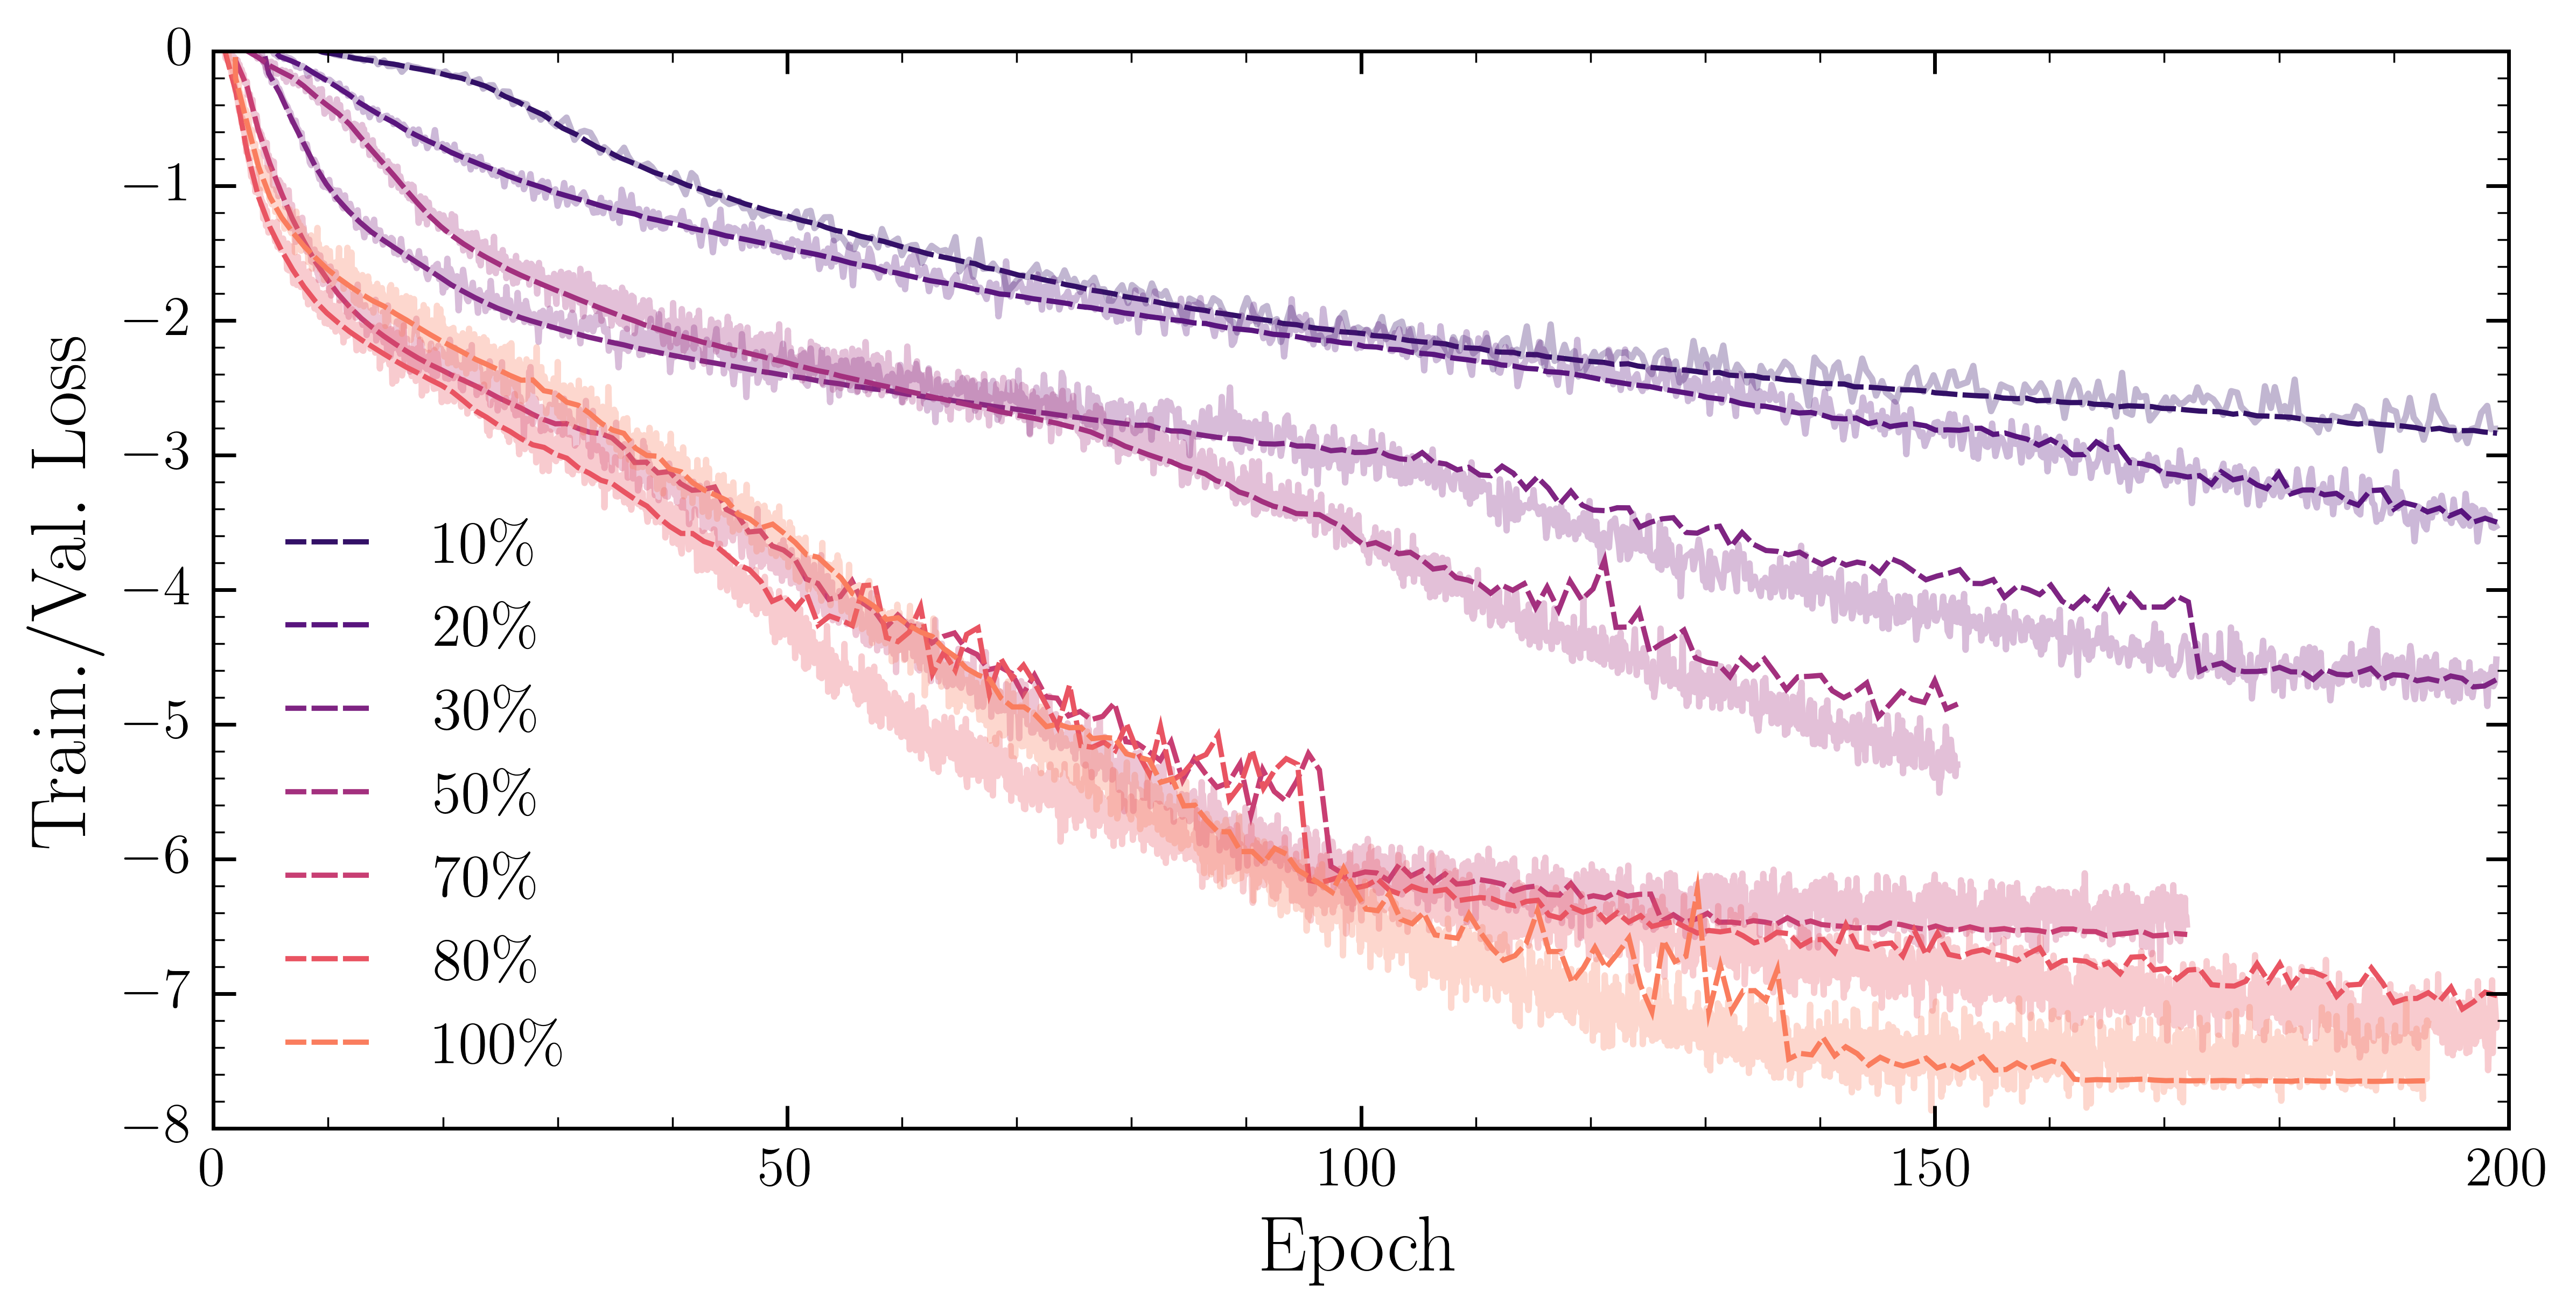
\includegraphics[width=\linewidth]{ANRE-loss_test.png}
    \caption{Training loss for order B (see Figure~\ref{fig:corner_streams_2} and Section~\ref{subsec:anre-stream} and Figure~\ref{fig:streams_loss} in the main text) as a function of epochs for different simulation budgets, with a maximum budget of $6\times 10^5$ simulations. The validation loss for each case is shown as a dashed line in the figure.}
    \label{fig:anre-training}
\end{figure}

\section{Gravitational lensing experiment}
\label{apx:anre-lensing}

 In this appendix we provide a more detailed account of the model adopted to generate the strong lensing simulations, the training details, and the employed neural networks to obtain the results presented in Section~\ref{subsec:lensing}.

\subsection{Simulator}

\begin{table}
    \centering
    \renewcommand{\arraystretch}{1.2}
    \begin{tabular}{c c c c c c c}
        \hline
        Component & Parameter & True value & Initial prior  \\
        \hline
        \parbox[t]{1mm}{\multirow{3}{*}{\rotatebox[origin=c]{90}{Subhalo}}}
        & $x_\mathrm{sub}\, ['']$ & -1.2 & $\mathcal{U}(-2.5, 2.5)$ \\
        & $y_\mathrm{sub}\, ['']$ & 1 & $\mathcal{U}(-2.5, 2.5)$ \\
        & $\log_{10} m_\mathrm{sub}\, [M_\odot]$ & $9.5$ & $\mathcal{U}(8, 11)$ \\
        \hline
        \parbox[t]{1mm}{\multirow{6}{*}{\rotatebox[origin=c]{90}{SPLE}}}
        & $x_\mathrm{lens}\, ['']$ & 0.1 & $\mathcal{U}(-0.2, 0.2)$  \\
        & $y_\mathrm{lens}\, ['']$ & 0.05 & $\mathcal{U}(-0.2, 0.2)$ \\
        & $\varphi_\mathrm{lens} \, [^\circ]$ & 0.3 & $\mathcal{U}(0, 1.5)$ \\
        & $q_\mathrm{lens}$ & 0.89 & $\mathcal{U}(0.1, 1)$ \\
        & $\gamma$ & 2 & $\mathcal{U}(1.8, 2.2)$ \\
        & $r_\mathrm{ein}\, ['']$ & 1.5 & $\mathcal{U}(1, 2)$ \\
        \hline
        \parbox[t]{1mm}{\multirow{2}{*}{\rotatebox[origin=c]{90}{Shear}}}
        & $\gamma_1$ & 0.01 & $\mathcal{U}(-0.05, 0.05)$  \\
        & $\gamma_2$ & -0.02 & $\mathcal{U}(-0.05, 0.05)$ \\
        \hline
        \parbox[t]{1mm}{\multirow{7}{*}{\rotatebox[origin=c]{90}{Lens light}}}
        & $x_\mathrm{light}\, ['']$ & 0.03 & $\mathcal{U}(-0.1, 0.1)$ \\
        & $y_\mathrm{light}\, ['']$ & 0.02 & $\mathcal{U}(-0.1, 0.1)$ \\
        & $\varphi_\mathrm{light} \, [^\circ]$ & 0.3 & $\mathcal{U}(0., 1.5)$ \\
        & $q_\mathrm{light}$ & 0.7 & $\mathcal{U}(0.1, 1)$ \\
        & $n$ & 1.58 & $\mathcal{U}(0.1, 4)$ \\
        & $r_e\, ['']$ & 2.1 & $\mathcal{U}(0.1, 3)$ \\
        & $I_e$ & 1.2 & $\mathcal{U}(0, 4)$ \\
        \hline
        \parbox[t]{1mm}{\multirow{7}{*}{\rotatebox[origin=c]{90}{Source light}}}
        & $x_\mathrm{src}\, ['']$ & 0.02 & $\mathcal{U}(-0.2, 0.2)$ \\
        & $y_\mathrm{src}\, ['']$ & 0.08 & $\mathcal{U}(-0.2, 0.2)$ \\
        & $\varphi_\mathrm{src} \, [^\circ]$ & 0.7 & $\mathcal{U}(0., 1.5)$ \\
        & $q_\mathrm{src}$ & 0.8 & $\mathcal{U}(0.1, 1)$ \\
        & $n$ & 1.5 & $\mathcal{U}(0.1, 4)$ \\
        & $r_e\, ['']$ & 1.4 & $\mathcal{U}(0.1, 3)$ \\
        & $I_e$ & 2.5 & $\mathcal{U}(0, 4)$ \\
        \hline
    \end{tabular}
    \caption{True subhalo and macro-model parameter values and priors used in the first \gls*{tmnre} inference round in the strong gravitational lensing application. This prior generates images with variance displayed in the first row of Figure~\ref{fig:targeted_data}.}
    \label{tab:anre-lensing-params}
\end{table}

We use the simulator adopted in Refs.~\cite{Coogan:2020yux, Coogan:2022cky, Montel:2022fhv}, and described in Section~\ref{sec:sl-model} to generate strong lensing image observations. To model the lens light and the source light flux we use a Sèrsic profile \cite{Sersic:1963aa}, parameterized by seven variables: position, position angle, axis ratio, index, effective radius, and surface intensity. We adopt a singular power-law ellipsoid (SPLE) \cite{Suyu:2008zp} for the main lens mass distribution, with a total of six parameters: position on the lens plane, position angle, axis ratio, slope, and Einstein radius. We consider two additional parameters to model the external shear. In total, there are twenty-two macro-model parameters. To model the density profile of the dark matter subhalo we adopt the smoothly truncated universal Navarro-Frenk-White mass density profile from Ref.~\cite{Baltz:2007vq}. We fix the truncation radius to $\tau=6$. The subhalo is then described by three parameters: virial mass $m_\mathrm{sub}$, and position on the lens plane $(x_\mathrm{sub}, y_\mathrm{sub})$. We adopt the concentration-mass relation from \cite{Correa:2015dva}. We show each parameter prior and the value with which we have generated our mock target observation in Table~\ref{tab:anre-lensing-params}.

Given this model, we generate $100 \times 100$ pixel$^2$ images with a resolution of $0.05"$ per pixel side, for a total field of view of $5" \times 5"$ in an image. The instrumental effects include a Gaussian point spread function with a full width at half maximum of $0.05"$ and Gaussian noise. We choose redshift $z_\mathrm{lens}=0.9$ for the lens and $z_\mathrm{source}=2$ for the source.

\subsection{Training details and neural networks}

\begin{table}
    \centering
    \begin{tabular}{c}
        \hline
        \texttt{Conv2d(1, 4, 3, 2, 1, bias=True)} \\
        \texttt{BatchNorm2d(4)} \\
        \texttt{ReLU} \\
        \hline
        \texttt{Conv2d(4, 8, 5, 2, 1, bias=True)} \\
        \texttt{BatchNorm2d(8)} \\
        \texttt{ReLU} \\
        \hline
        \texttt{Conv2d(8, 16, 5, 2, 1, bias=True)} \\
        \texttt{BatchNorm2d(16)} \\
        \texttt{ReLU} \\
        \hline
        \texttt{Conv2d(16, 32, 5, 2, 1, bias=True)} \\
        \texttt{BatchNorm2d(32)} \\
        \texttt{ReLU} \\
        \hline
        \texttt{Flatten()} \\
        \texttt{LazyLinear(256)} \\
        \hline
    \end{tabular}
    \caption{The convolutional compression network used in the macro-model parameter ratio estimator. The notation is taken from \texttt{PyTorch}: the arguments to \texttt{Conv2d} are the number of input channels, output channels, kernel size, stride and padding, respectively. The horizontal lines highlight where the number of channels changes. Note that we standardize the images before providing them to the convolutional networks.}
    \label{tab:anre-macro}
\end{table}
%
\begin{table}
    \centering
    \begin{tabular}{r l}
        \hline
        \texttt{image\_size} & \texttt{100} \\
        \texttt{n\_channels} & \texttt{1} \\
        \texttt{n\_classes} & \texttt{8}\\
        \texttt{s} & \texttt{1} \\
        \hline
    \end{tabular}
    \caption{The details of the UNet network used in the subhalo. We use the implementation from \url{https://github.com/milesial/Pytorch-UNet}, with arguments given in the table. The UNet output is then sampled at the positions of the subhalo contrastive examples to bring it to a lower dimensionality, and this feature vector is passed to the binary classifier.
    }
    \label{tab:anre-UNet}
\end{table}

 For all tasks we use the same general ratio estimator architecture. It consists of an initial compression network that maps the high-dimensional lensing observation $\data$ into a feature vector. This feature vector is concatenated to the parameters we want to infer. The vector is then passed to  \texttt{swyft} binary classifier which outputs an estimate of the likelihood-to-evidence ratio. The compressor architecture for the macro-model parameters is given in Table~\ref{tab:anre-macro}. This same compression is used when estimating 1-dimensional marginal ratio estimators, or the joint one with \gls*{nre} or autoregressive \gls*{nre}, as explained in Section~\ref{subsec:lensing}. The compressor architecture for the subhalo parameters is given in Table~\ref{tab:anre-UNet}.

We used the Adam optimizer with an initial learning rate of $10^{-3}$ for the macro-model ratio estimator and $8 \times 10^{-5}$ for the subhalo ratio estimator, and a batch size of $64$. The learning rate was reduced by a factor of $0.1$ whenever the validation loss plateaued for $2$ epochs. Training was run until the validation loss stopped improving for more than $5$ epochs. The results shown in Figure~\ref{fig:corner} are obtained using $2\times 10^5$ training samples. To run the inference, we use the model weights obtained at the lowest validation loss curve point.

\end{subappendices}

%\chapter{Simulation-based inference for cosmological initial conditions} \label{cha:cosmo}

Reconstructing astrophysical and cosmological fields from observations is challenging. It requires accounting for non-linear transformations, mixing of spatial structure, and noise. In contrast, forward simulators that map fields to observations are readily available for many applications. In this chapter, we present a versatile Bayesian field reconstruction algorithm rooted in \gls*{sbi} and  enhanced by autoregressive modeling. The proposed technique is applicable to generic (non-differentiable) forward simulators and allows sampling from the posterior for the underlying field. We show first promising results on a proof-of-concept application: the recovery of cosmological initial conditions from late-time density fields.

\textit{This chapter is based on work from \cite{List:2023aa}.}


\section{Introduction} \label{sec:cosmo-intro}

Recent developments in simulation-based machine learning are increasingly used for tackling difficult astrophysical and cosmological data analysis challenges~\cite[\eg,][]{Mishra-Sharma:2021oxe,
Cole:2021gwr, Alvey:2023npw, AnauMontel:2023stj, AnauMontel:2022ppb, Montel:2022fhv, Alsing:2017var, Alsing:2019dvb, Alsing:2019xrx, Makinen:2021nly, Modi:2023drt, Modi:2023llw, Barrue:2023ysk, Heinrich:2023bmt, Lin:2022ayr, Gagnon-Hartman:2023soa, Poh:2022ife, Lemos:2022kua, Brehmer:2019jyt, Alvey:2023naa, Bhardwaj:2023xph, Alvey:2023pkx, Karchev:2022xyn, Crisostomi:2023tle, Campeau-Poirier:2023kqd, Coogan:2022cky, Hahn:2022wgo, Jeffrey:2020aa, Saxena:2023tue}.
While \gls*{sbi} has primarily been employed to solve relatively low-dimensional ($\lesssim 50$-dimensional) parameter estimation tasks~\cite{AnauMontel:2023stj, Alvey:2023naa, Alsing:2019xrx}, it has yet to cover higher-dimensionality problems like image reconstruction, which are an essential component in astrophysical and cosmological data analysis. 

Here, we focus on the recovery of cosmological initial conditions from late-time density fields. This task is a challenging test case for new algorithms thanks to the non-linear, non-local mapping from the Gaussian target to the observation.  Cosmic inflation predicts the density in the early universe to be highly homogeneous, with tiny density fluctuations that are extremely well described as a Gaussian random field. These density perturbations then gradually grow over cosmic time due to gravity and eventually collapse into the non-Gaussian ``Cosmic Web'' structure observed today \cite{Bond:1995yt}. 
The reconstruction of the initial density field from late-time observations is an ill-posed problem (the early-to-late mapping is not injective on small scales, ~\cite[\eg,][]{Brenier:2003xs}). Therefore, there is an entire {\it distribution} of possible initial conditions consistent with a given late-time density field. 

\paragraph{Our contribution.}  We frame the task of field reconstruction (or, viewed from a non-physical point of view, image reconstruction) as a parameter inference problem.  We combine the power of \gls*{sbi} in solving parametric inverse problems together with the scalability offered by autoregressive models. Autoregressive models have established their versatility in tackling high-dimensional distribution estimation tasks by breaking down the joint distribution into a product of conditionals \cite{Papamakarios:2017tec, Uria:2016aa}, and have been successful in conditional image modeling \cite{van:2016pixel}. Additionally, we employ a Gibbs sampling algorithm based on exact data augmentation (GEDA) \cite{Marnissi:2019aa} to efficiently sample image parameter posteriors.
We will formulate our method in a generic way to emphasize its applicability to a wide range of field/image reconstruction problems. Importantly, our approach accommodates arbitrary \textit{non-differentiable} forward simulators.

\paragraph{Related work.} The problem of inferring cosmological initial conditions has been studied since the late 1980s (see \eg~Refs.~\cite{Croft:1996jw, Frisch:2001vw, Gramann:1993aa, Nusser:1992aa, Peebles:2020aa, Weinberg:1992aa} for classical papers), for instance by applying the least-action principle or using optimal transport. In the last decade, Bayesian models have been formulated for this task ~\cite[\eg,][]{Jasche:2012kq}, many of which rely on differentiable forward models \cite{Li:2022bsu, Modi:2020dyb}, in conjunction with Hamiltonian Monte Carlo sampling. 
Recently, machine learning methods such as convolutional neural networks \cite{Shallue:2022mhf, Chen:2023uup}, variational inference \cite{Modi:2022pzm}, recurrent inference machines \cite{Modi:2021acq}, and score-based modeling \cite{Legin:2023jxc} have also been explored in this context. 


\section{Methodology} \label{sec:cosmo-method}

We structure our methodology as follows. First, in Section~\ref{subsec:cosmo-setup}, we set up the problem in terms of a simple hierarchical field simulator. We then introduce this work's main contribution: autoregressive gaussian likelihood estimation (Section~\ref{subsec:cosmo-auto}) and high-dimensional gaussian posterior sampling through GEDA (Section~\ref{subsec:cosmo-geda}).


\subsection{Problem setup} \label{subsec:cosmo-setup}

%\subsection{Background and problem setup} 

%\Gls*{sbi} methods tackle statistical inverse problems by estimating posterior distributions from model-simulations. These methods do not require explicit modeling of the data likelihood, but instead access the information within the likelihood indirectly via a stochastic simulator, which maps input parameters to simulated data. Among various \gls*{sbi} algorithms (see Ref.~\cite{Cranmer:2019eaq} for a review and Ref.~\cite{Lueckmann:2021aa} for benchmarks), we will focus on \gls*{nre}, which rephrases posterior estimation into a binary classification problem \cite{Hermans:2019ioj, Miller:2021aa}.

Let us assume we have a simple hierarchical simulator
\begin{equation}
    p(\data| \interest)p(\interest)
\end{equation}
where $\data\in \mathbb{R}^{N \times N}$ is observed and $\interest\in \mathbb{R}^{N \times N}$ are image parameters (pixel values). Here, $p(\data|\interest)$ can include non-linear, non-local transformations and non-Gaussian noise, and it is only implicitly defined through a forward simulator. We will discuss how we can, for a given observation $\data_o$, estimate an approximate but computationally efficient Gaussian likelihood that locally resembles $p(\data_o|\interest)$ for a target observation $\data_o$. 
A fast surrogate can then be leveraged for downstream image analysis tasks.


\subsection{Autoregressive gaussian likelihood estimation} \label{subsec:cosmo-auto}

Firstly, in order to obtain locally optimal data summaries $\bm s(\data)$ for the image reconstruction task, we use \gls*{nre} to estimate the marginal, pixel-wise ratios\footnote{~In this work we use the following notation for ratio estimators $\hat r(a;b) = \frac{p(a,b)}{p(a)p(b)} = \frac{p(a|b)}{p(a)}$. If necessary, multiple variables are comma separated,
for example $\hat r(a; b, c)=\frac{p(a,b,c)}{p(a)p(b, c)}$.}
\begin{equation}
    \hat r(s_i(\data); \theta_i) \equiv \frac{p(s_i , \theta_i)}{p(s_i)p(\theta_i)} \;.
\end{equation}
We assume here that both the joint and marginal distributions can be approximated as Gaussians, whereas the mapping $s_i(\data)$ is an arbitrary learnable function (usually a neural network). 
Means and covariances are estimated on-the-fly during training (similarly to batch normalization \cite{Ioffe:2015ovl}) and are not represented as learnable parameters.
Secondly, in order to obtain an estimate of the joint likelihood $p(\data|\interest)$, we proceed as follows.  We split the problem auto-regressively along the observation axis, and we use \gls*{nre} to estimate
\begin{equation} \label{eq:cosmo-autoregressive}
\begin{split}
        \frac{p(\data| \interest)}{p(\data)} &\simeq \frac{p(\bm s(\data)| \interest)}{p(\bm s(\data))} = \prod_{i=1}^{N^2} \frac{p(s_i| \bm s_{1:i-1}, \interest)}{p(s_i| \bm s_{1:i-1})} \\
        &\simeq \prod_{i=1}^{N^2}  \hat r(s_i; l_i, \theta_i) = \prod_{i=1}^{N^2} \frac{p(s_i, l_i, \theta_i)}{p(s_i)p(l_i, \theta_i)} \;,
\end{split}
\end{equation}
where we have introduced $l_i = (\bm L(\bm s))_i$ with $\bm L$ a (generally non-linear) autoregressive function.
Again, we assume that the individual functions $p(s_i, l_i, \theta_i)$ are (three-dimensional multivariate) Gaussians.

By rewriting the above components (for a complete derivation and definitions of $\bm Q_{\text{like}}$ and $\bm b$ see Appendix~\ref{apx:info}), we can obtain the likelihood function in the so-called \emph{information form},
\begin{equation}\label{eq:cosmo-likelihood}
    \ln p(\data|\interest) = -\frac12 \interest^T \bm Q_{\text{like}} \interest + \bm b \interest + C(\bm s) \;.
\end{equation}
In this paper, we assume that the precision matrix $\bm Q_{\text{like}}$ is diagonal. However, correlations between data summaries $\bm s$ are accounted for through the autoregressive function mentioned above; also, each component $s_i(\data)$ of the data summary may depend on all components of $\data$ and thus accounts for cross-pixel information.

To enhance the robustness of Bayesian approaches in data analysis, frequently likelihood tempering techniques are employed that result in conservative estimates \cite{Holmes:2017aa, Jasche:2019aa}. 
Tempering the likelihood amounts to raising it to a fractional power $\gamma \in [0, 1]$, leading to progressively coarser posterior samples, with the extreme case of $\gamma=0$ ($\gamma = 1$) corresponding to samples drawn from the prior (posterior) distribution.


\subsection{High-dimensional gaussian posterior sampling} \label{subsec:cosmo-geda}
In our Bayesian framework and assuming Gaussian distributions, we combine the estimated likelihood with the known prior to derive the posterior in the information form
\begin{equation} \label{eq:cosmo-post}
    \ln p(\interest|\data) = -\frac12 \interest^T \underbrace{(\bm Q_{\text{like}}+\bm Q_{\text{prior}})}_{\bm Q_{\text{post}}} \interest + \bm b \interest + C'(\bm s) \;, 
\end{equation}
where we have assumed a zero-mean prior, consistent with the physical problem we study in Section~\ref{sec:cosmo-exp}.
We use the conjugate gradient (CG) algorithm\footnote{~We use a slightly modified implementation of the preconditioned CG algorithm from \url{https://github.com/sbarratt/torch_cg}.} 
to compute the maximum-a-posteriori (MAP) estimate $\interest_{\text{MAP}}$ of the image parameters $\interest$ by solving the linear system $\bm Q_{\text{post}} \interest = \bm b$.
The surrogate Gaussian posterior distribution is then given by $p(\interest | \data) = \mathcal{N}(\interest_{\text{MAP}}, \bm Q_{\text{post}}^{-1})$.
Once we have the posterior distribution in the above form, we simply have to sample from it.
Various techniques have been presented over time to tackle the problem of efficient sampling from a high-dimensional Gaussian distribution (for a recent review, see Ref.~\cite{Vono:2020aa}). 
To obtain the Gaussian posterior samples, we use a Gibbs sampler based on the generalized exact data augmentation algorithm 
(GEDA)~\cite{Marnissi:2019aa}. GEDA solves the problem of high-dimensional Gaussian sampling specifically for distributions whose precision matrix can be expressed as $\bm Q = \bm Q_1 + \bm Q_2$ by exploiting specific properties of $\bm Q_1$ and $\bm Q_2$. Crucially, $\bm Q_{\text{post}}$ satisfies these constraints.

In general, data augmentation approaches target precision matrices of the form $\bm Q = \bm Q_1 + \bm Q_2$, which naturally arise from the statistical model under investigation.  Taking advantage of potential specific structures of $\bm Q_1$ and $\bm Q_2$, data augmentation strategies introduce one (or several) auxiliary variable $\bm u \in \mathbb R^d$ such that the joint distribution of the pair $(\bm u, \interest)$ yields simple conditional distributions, thus sampling steps for a Gibbs sampler. One can recover the target distribution $\mathcal{N}(\bm \mu, \bm Q^{-1})$ via marginalization of the auxiliary variable $\bm u$, either exactly (as in exact data augmentation schemes, like GEDA) or in an asymptotic regime.

In GEDA, as described in Ref.~\cite{Marnissi:2019aa}, the underlying assumption is that the precision matrix $\bm Q$ can be split as follows:
\begin{equation}
\begin{split}
    & \bm Q = \bm Q_1 + \bm Q_2 \\
    & \bm Q_1 = \bm G_1^T \bm D_1 \bm G_1 \\
    & \bm Q_2 = \bm U_2^T \bm D_2 \bm U_2 \,,
\end{split}
\label{eq:cosmo-precision_split}
\end{equation}
where $\bm G_1$ is arbitrary, $\bm D_1$ is diagonal and positive definite, $\bm U_2$ is unitary, and  $\bm D_2$ is diagonal. 
GEDA introduces two auxiliary variables, $\bm u_1$ and $\bm u_2$, such that the joint distribution is
\begin{equation}
\begin{split}
    p(\interest, \bm u_1, \bm u_2) \propto & \exp\left(-\frac{1}{2}\left[(\interest-\bm\mu)^T \bm Q(\interest-\bm\mu) + (\bm u_1 - \interest)^T \bm R(\bm u_1 - \interest)\right] \right) \\
    &\times \exp\left( -\frac{1}{2}(\bm u_2-\bm G_1 \bm  u_1)^T \bm D_1(\bm u_2-\bm G_1 \bm  u_1)\right) \,,
\end{split}
\end{equation}
where $\bm R = \omega^{-1} \bm I_d - \bm Q_1$, and  $\omega$ is a positive hyper-parameter of the algorithm that must obey $1 < \omega < 1/ \lvert \bm Q_1 \rvert$, meaning that $1/\omega$ should be larger than the largest singular value of $\bm Q_1$. 

This joint distribution yields conditional Gaussian distributions with diagonal covariance matrices for both $\bm u_1$ and $\bm u_2$ that can be sampled efficiently by a Gibbs sampler with the following steps:
\begin{equation}
\begin{array}{ccl}
    1. & \bm u_2\sim\mathcal{N}(\bm \mu_{\bm u_2}, \bm Q^{-1}_{\bm u_2}) & \text{with } \bm \mu_{\bm u_2} = \bm G_1 \bm u_1 \text{ and }\bm Q_{\boldsymbol u_2} = \boldsymbol D_1, \\
    2.  & \bm u_1\sim\mathcal{N}(\bm \mu_{\bm u_1}, \bm Q^{-1}_{\bm u_1})  & \text{with } \bm \mu_{\bm u_1} = \interest - \omega(\bm Q_1 \interest - \bm G_1^T \bm D_1^{-1} \bm u_2) \text{ and } \bm Q_{\bm u_1} = \omega^{-1} \bm I_d, \\
    3.  & \bm u_1\sim\mathcal{N}(\bm \mu_{\bm u_1}, \bm Q^{-1}_{\bm u_1}) & \text{with }\bm \mu = \bm Q(\bm R \bm  u_1 + \bm  Q \bm \mu) \text{ and } \bm Q = \omega^{-1} \bm I_d + \bm Q_2 \;.
\end{array}
\end{equation}

In our setup the dimensionality is equivalent to the number of pixels $d=N^2$, the covariance matrix is $\bm Q = \bm Q_{\text{post}} = \bm Q_{\text{like}} + \bm Q_{\text{prior}}$, and $\bm G_1= \bm I$.


\section{Experiment} \label{sec:cosmo-exp}
\begin{figure}
    \centering
    \resizebox{0.8\textwidth}{!}{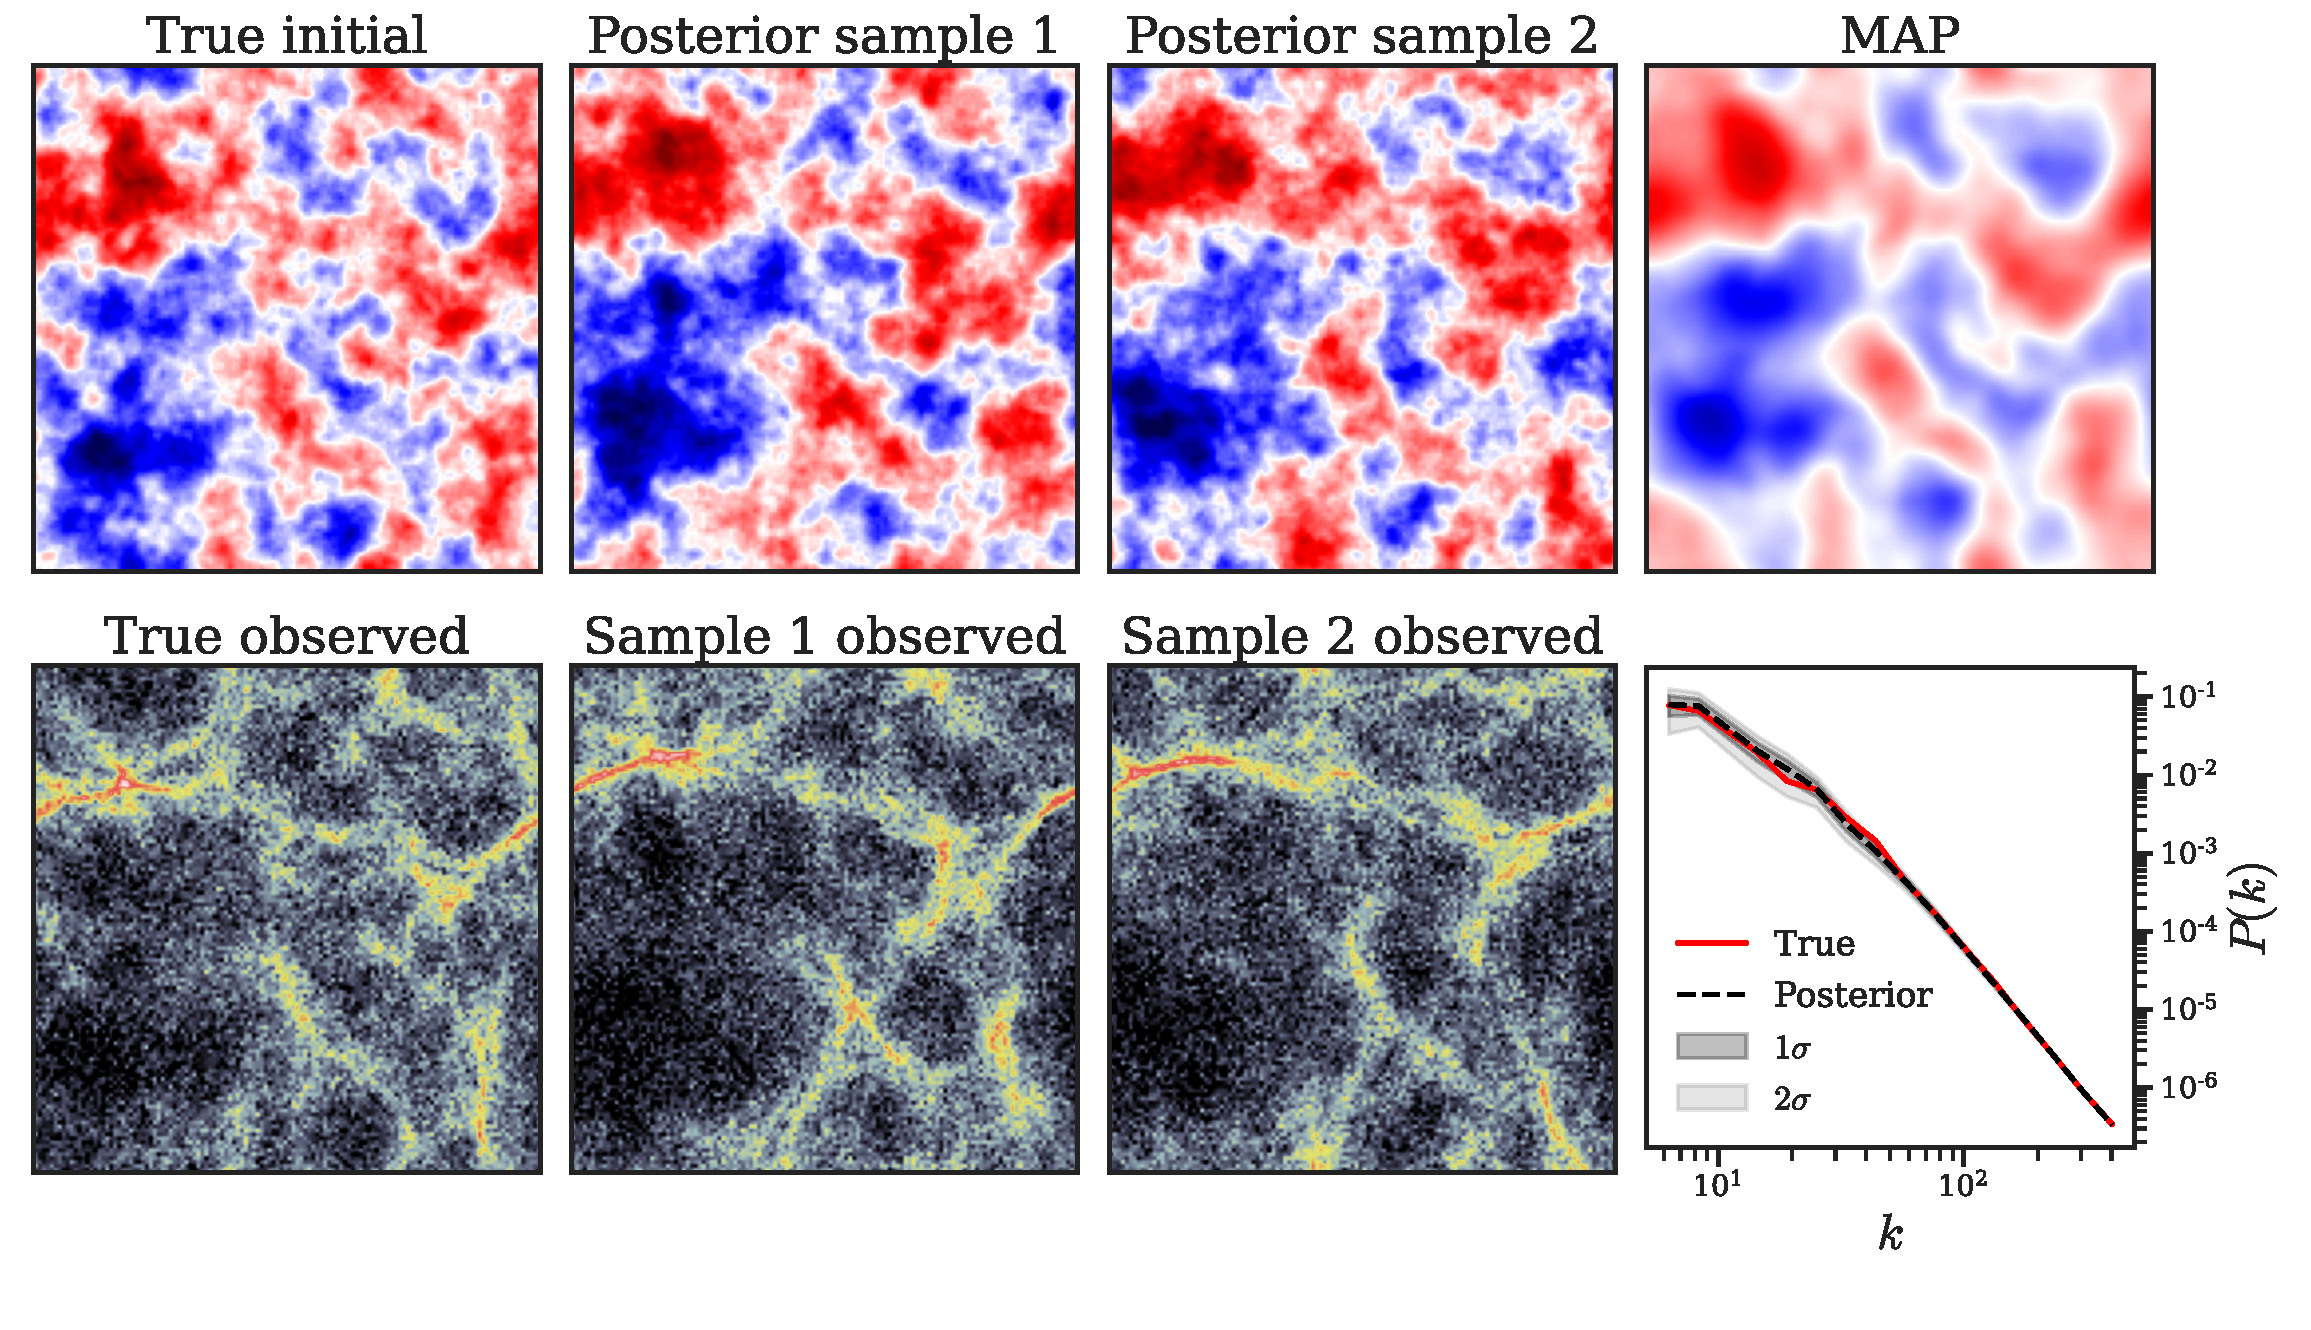
\includegraphics{ANRE-cosmo-result_with_2_samples.pdf}}
    \caption{Reconstruction of cosmological initial conditions in 2D. {\it Top left:} True initial density~${\interest}_o$. {\it Bottom left}: True observation ${\data}_o$, \ie\ the (logarithm of the) late-time density evolved from the initial conditions ${\interest}_o$, corrupted by uncorrelated Gaussian noise. {\it Top center:} Two samples drawn from the posterior $p(\interest | \bm {\data}_o)$. {\it Bottom center:} Observations computed from the posterior samples shown above. {\it Upper right:} Maximum-a-posteriori probability (MAP) estimate ${\interest}_{\text{MAP}}$ of the initial conditions. {\it Bottom right:} Distribution of the reconstructed initial power spectrum.}
    \label{fig:results}
\end{figure} 

To demonstrate the efficiency of our method, we apply it to the task of reconstructing the initial conditions of the universe. 

\paragraph{Forward model.} In this proof-of-concept study, we consider the two-dimensional case and assume Einstein--de Sitter cosmology (\ie\ non-relativistic, collisionless matter only). While our framework readily supports marginalizing over image parameters such as the power spectra of the target fields, we use a fixed power-law power spectrum for the initial density contrast $\interest = \bm \delta_{\mathrm{ini}} \in \mathbb{R}^{128 \times 128}$, which is the target of our inference.
As a forward model, we use second-order Lagrangian perturbation theory (2LPT, see Refs.~\cite{Bouchet:1992aa, Buchert:1993aa} and Appendix~\ref{apx:2lpt}) and evolve the initial density to a time when non-linear structures have formed. The observation is then given by $\data = \log_{10}[1.1 + {\bm \delta}_{\mathrm{final}}] + \bm \varepsilon$, where ${\bm \delta}_{\mathrm{final}}$ is the density contrast at final time, the logarithm is applied element-wise, and we add $\bm \varepsilon \sim \mathcal{N}(\bm 0, \sigma^2 \bm I)$ with $\sigma = 0.15$ as a simplistic model for observational noise.

\paragraph{Training strategy.}To obtain pixel-wise summaries $\bm{s}(\data)$, we use a standard U-Net \cite{ronneberger:2015u}. In our current implementation, we use an autoregressive convolution ~\cite[\eg,][]{van:2016pixel} as the autoregressive function $\bm L$. In our experiments, we observed that overly small or large kernel sizes result in somewhat biased posteriors. Interestingly, we obtain the best results with a physically motivated kernel size for the convolution, \ie\ when choosing it in such as way that the ``radius of influence'' of the autoregressive convolution (\ie\ roughly half the kernel size) matches the typical distance that particles (or fluid elements)
have traveled by the end time -- a quantity known as displacement. Specifically, the mean displacement in our case is $\sim 5$ pixels, so we take the kernel size to be $11 \times 11$ pixels. While we find this choice to be optimal, slight bias still occurs occasionally, potentially due to the spatial heterogeneity of the displacements. Therefore, to be conservative, we use a tempered likelihood with $\gamma = 0.5$, trading some of the statistical constraining power of our method for increased unbiasedness. The importance of the specific choice of $\bm L$ (and in particular its radius of influence) indicates that a locally adaptive or multi-scale approach for $\bm L$ is a promising avenue for future exploration. We train our model on 1000 $(\data, \interest)$-pairs for 15 epochs, which only takes $\sim 3$ minutes on a laptop GPU for this experiment. Obtaining the MAP estimate with the CG algorithm takes less than 3 seconds. To obtain posterior samples with GEDA, we perform 300 sampling steps, which takes $<$ 1 second per sample (and multiple samples can be drawn in batches).

\paragraph{Results.}The left column of Figure~\ref{fig:results} shows a target initial density contrast ${\interest}_o$ ({\it top}), together with a resulting noisy observation at late time ${\data}_o$ ({\it bottom}). In the two center panels, we plot samples drawn from the (tempered) posterior $p(\interest | {\data}_o)$, together with an observation of each sample. The upper right panel shows the MAP estimate ${\interest}_{\text{MAP}}$. The initial density field is faithfully reconstructed on large scales whereas, as expected, small-scale information remains unconstrained. Finally, the lower right panel shows that the power spectra of the posterior samples are consistent with the target field. The excellent agreement between reconstructed and true power spectra on small scales is aided by the fact that the power spectrum (which is fixed in our example) directly enters the GEDA sampling (see Equation~\ref{eq:cosmo-precision_split} in Section~\ref{subsec:cosmo-geda}, where the prior precision matrix ${\bm Q}_2$ is diagonalized by the Fourier transform, with the power spectrum on the diagonal of ${\bm D}_2$). We will present a detailed quantitative analysis of the results obtained with our framework in a separate publication.

\section{Discussion and conclusions} \label{sec:cosmo-conc}
We have introduced a framework for Bayesian field/image reconstruction by combining \gls*{sbi}, autoregressive modeling, and a Gibbs sampling algorithm based on exact data augmentation (GEDA). We presented promising results for a toy example related to reconstructing the initial conditions of the universe. In view of its \textit{remarkable speed, low simulation costs, and the fact that it works for general non-differentiable simulators}, we expect our method to be capable of handling significantly higher-dimensional problems, including 3D cosmological simulations.

There are multiple promising avenues to be explored in future work. For many applications---such as the reconstruction of cosmological initial conditions---formulating the problem in Fourier space can be expected to produce significantly tighter posteriors, as the input-to-output mapping is exactly invertible on large to intermediate scales, and the stochasticity of the reconstruction only affects small scales. Alternatively, wavelets ~\cite[\eg,][]{graps:1995introduction} or other multiscale techniques could be exploited.
In this context (but also more generally), other choices for the autoregressive function $\bm L$ are worthwhile exploring, which could, for instance, implement the hierarchy between the different scales. 
Another promising enhancement involves harnessing the sequential aspect of \gls*{sbi} techniques. In principle, a viable strategy is to employ an adaptive scheduler to control the value of $\gamma$ to draw new training samples for sequential inference rounds.
Moreover, being \gls*{sbi}-based, our proposed method is capable of marginalizing over cosmological parameters or, alternatively, infer them in addition to the phases of the initial random field.

Let us also comment on the current limitations of our method: while the assumption of Gaussianity for the prior is justified for reconstructing cosmological initial conditions, using a Gaussian likelihood is an approximation whose justification depends on the specific task at hand. We take cross-pixel information into account through the summary statistics and an autoregressive function, but we currently model the precision matrix of the likelihood as being diagonal. In addition, the susceptibility of our framework to issues encountered in the context of autoregressive models such as exposure bias \cite{bengio:2015scheduled} merits further investigation.

Finally, we remark that the forward model generating ``observations'' $\data$ does not necessarily need to be a physical one, and our framework also holds great promise for generic image reconstruction problems consisting in inferring one image from another.


%   \section*{Acknowledgments and Disclosure of Funding}
%    This work is part of a project that has received funding from the European Research Council (ERC) under the European Union’s Horizon 2020 research and innovation program (Grant agreement No. 864035 -- UnDark). FL thanks Oliver Hahn and Cornelius Rampf for many insightful discussions.


%%%%%%%%%%%%%%%%%%%%%%%%

\begin{subappendices}

\section{Derivation of the likelihood in the information form} \label{apx:info}

In this appendix we show how to derive the quadratic term $\bm Q_\text{like}$ and the linear term $\bm b$ of the likelihood in the information form (Equation~\ref{eq:cosmo-likelihood}) starting from Equation~\ref{eq:cosmo-autoregressive}. Having approximated $p(s_i, l_i, \theta_i)$ with a 3-dimensional Gaussian distribution, we can write the log-likelihood as
%
\begin{equation}
    \ln p(\bm s(\data)| \interest) = \sum_{i=1}^{N^2} \ln \frac{p(s_i, l_i, \theta_i)}{p(l_i, \theta_i)} = \sum_{i=1}^{N^2} \ln \frac{\mathcal{N}(\mu_{(s_i, l_i, \theta_i)}, \Sigma_{(s_i, l_i, \theta_i)})}{\mathcal{N}(\mu_{(l_i, \theta_i)}, \Sigma_{(l_i, \theta_i)})} \;.
\end{equation}
%
Let us consider just one element $i$ and drop the index $i$ for simplicity of notation. Expanding the above expression for one component, we obtain
%
\begin{equation}\label{eq:cosmo-matrix}
\begin{split}
    & -\frac12
    \begin{pmatrix}
    s-\mu_s \\
    l-\mu_l \\ 
    \theta-\mu_\theta \\
    \end{pmatrix}^T\hspace{-3mm}
    \underbrace{
    \begin{pmatrix}
    \Sigma_{ss} & \Sigma_{sl} & \Sigma_{s\theta} \\
    \Sigma_{ls} & \Sigma_{ll} & \Sigma_{l\theta} \\
    \Sigma_{\theta s} & \Sigma_{\theta l} & \Sigma_{\theta \theta}
    \end{pmatrix}^{-1}}_{
    \equiv Q' = 
    \begin{pmatrix}
    Q'_{ss} & Q'_{sl} & Q'_{s\theta} \\
    Q'_{ls} & Q'_{ll} & Q'_{l\theta} \\
    Q'_{\theta s} & Q'_{\theta l} & Q'_{\theta \theta}
    \end{pmatrix}
    }\hspace{-3mm}
    \begin{pmatrix}
    s-\mu_s \\
    l-\mu_l \\ 
    \theta-\mu_\theta 
    \end{pmatrix}
    +\frac12
    \begin{pmatrix}
    l-\mu_l \\ 
    \theta-\mu_\theta
    \end{pmatrix}^T\hspace{-3mm}
    \underbrace{\begin{pmatrix}
    \Sigma_{ll} & \Sigma_{l\theta} \\
    \Sigma_{\theta l} & \Sigma_{\theta \theta}
    \end{pmatrix}^{-1}}_{
    \equiv Q'' = 
        \begin{pmatrix}
    Q''_{ll} & Q''_{l\theta} \\
    Q''_{\theta l} & Q''_{\theta \theta}
    \end{pmatrix}\;
    }\hspace{-3mm}
    \begin{pmatrix}
    l-\mu_l \\ 
    \theta-\mu_\theta
    \end{pmatrix} 
    \;.
\end{split}
\end{equation}

For a specific observation $\data$ we can compute $\bm s$ and therefore $\bm l$, hence individual components $s$ and $l$ (where we have dropped the index $i$). We can then read off the expression in Equation~\ref{eq:cosmo-matrix} the terms that depend on $\theta$. We group the rest into an irrelevant constant $C(s)$.
In this way, the \textit{quadratic term} in $\theta$ in Equation~\ref{eq:cosmo-matrix} is
\begin{flalign*}
        -\frac12 Q_{\theta \theta}\theta^2 &\quad\text{with}\quad Q_{\theta \theta} \equiv Q'_{\theta \theta} - Q''_{\theta \theta} \;.
\end{flalign*}
Each $Q_{\theta \theta}$ is a diagonal entry of $\bm Q_\text{like}$ in Equation~\ref{eq:cosmo-likelihood}, while non-diagonal components are 0 by construction. In principle, correlations between pixels in the data $\data$ can be modeled and we plan to explore it in future work.
The \textit{linear term} in $\theta$ in Equation~\ref{eq:cosmo-matrix} is
\begin{equation}
    b  \equiv \left[-(s-\mu_s) Q'_{s\theta} -(l-\mu_l) Q_{l\theta} + \mu_\theta Q_{\theta \theta}\right] \;.
\end{equation}
Each component $b$ composes the likelihood linear term $\bm b$.
    
\section{Second-order Lagrangian perturbation theory (2LPT)}
\label{apx:2lpt}
Second-order Lagrangian perturbation theory (2LPT) describes the cosmological dynamics of a cold, collisionless medium. It is based on a fluid description of the Vlasov--Poisson system \cite[\eg][]{Peebles:2020aa} and therefore ceases to be valid as soon as particle trajectories cross (so-called ``shell-crossing''). Although the density fields we consider herein are well in the post-shell-crossing regime, 2LPT still serves as a suitable forward model for validating our image reconstruction method.

The central quantity in 2LPT is the displacement $\bm \psi(\bm q, a) = \bm p(\bm q, a) - \bm q$, \ie\ the vector pointing from each Lagrangian (``initial'') position $\bm q$ to the associated Eulerian position ${\bm p}({\bm q}, a)$ at scale-factor time $a$ on the characteristic curve originating at $\bm q$. LPT expands the displacement as a Taylor series w.r.t.\ $a$, with a purely space-dependent coefficient $\bm \psi^{(n)}(\bm q)$ at the $n$-th order. For 2LPT, this yields
\begin{equation}
    \bm \psi(\bm q, a) = a \bm \psi^{(1)}(\bm q) + a^2 \bm \psi^{(2)}(\bm q) \;,
\end{equation}
where 
\begin{subequations}
\begin{align}
    \bm \psi^{(1)} &= - \bm \nabla_{\bm q} \phi^0 \;, \\
    \bm \psi^{(2)} &= -\frac{3}{7} \bm \nabla_{\bm q} \, \Delta_{\bm q}^{-1} \left[(\partial_{q_1, q_1} \phi^0) \, (\partial_{q_2, q_2} \phi^0) - (\partial_{q_1, q_2} \phi^0)^2 \right] \;.
\end{align}
\end{subequations}
Here, $\phi^0$ is the initial gravitational potential, and the scale factor $a$ simply acts as a time variable and has no physical meaning in 2D.  Note that we consider Einstein--de Sitter cosmology ($\Omega_m = 1$); for extensions to the $\Lambda$CDM case and higher-order LPT, see \eg~Ref.~\cite{Rampf:2022tpg} and references therein.

Given the 2LPT displacement $\bm \psi$, the density contrast $\delta$ is given by
\begin{equation}
    1 + \delta(\bm p(\bm q, a)) = \int \delta_\text{D}(\bm p(\bm q, a) - \bm q - \bm \psi(\bm q, a)) \ \mathrm{d}^2q \;,
\end{equation}
where $\delta_\text{D}$ is the Dirac $\delta$-distribution. In practice, we use cloud-in-cell interpolation \cite[\eg][]{HockneyEastwood:1988} to compute the density contrast on a Cartesian grid. Finally, let us remark that since we view the discrete density contrast as an $N \times N$-dimensional image in the main part of this work, we use the bold symbol $\bm \delta$ in that context.

\end{subappendices}

%\chapter{Simulation-based inference for point sources} \label{cha:detection}

Statistical inference of population parameters of astrophysical sources is challenging. It requires accounting for selection effects, which stem from the artificial separation between bright detected and dim undetected sources that is introduced by the analysis pipeline itself. In this chapter, we show that these effects can be modeled self-consistently in the context of sequential \gls*{sbi}. Our approach couples source detection and catalog-based inference in a principled framework that derives from the \gls*{tmnre} algorithm. It relies on the realization that detection can be interpreted as prior truncation. We outline the algorithm, and show first promising results.

\textit{This chapter is based on work from \cite{AnauMontel:2022ppb}.}


\section{Introduction}
\label{sec:ps-intro}

Point sources detection is crucial for astronomical surveys, and is the cornerstone for the compilation of source catalogues. Those source catalogues are then typically the basis for the inference of physical parameters that describe the sources at the population level. Upcoming astronomical facilities, such as the Square Kilometer Array (SKA)~\citep{Weltman:2018zrl} and the Cherenkov Telescope Array (CTA)~\citep{CTAConsortium:2017dvg} will deliver large and complex datasets.  In order to leverage their full potential, it is urgent to develop robust and automated source detection and source population parameters inference algorithms.

Machine learning is a particularly promising tool to address this big data challenge. Recent developments in deep learning and more generally automatic differentiation frameworks~\citep{baydin2018automatic} are increasingly used for tackling difficult astronomical data analysis with the goal to extricate more information from the available data. The capability of deep learning techniques of point sources detection and population characterization has been demonstrated across different wavelengths surveys, \eg~in $\gamma$-ray data~\citep{Panes:2021zig, Caron:2017udl, List:2021aer, Mishra-Sharma:2021oxe}, radio data~\citep{VafaeiSadr:2018tac, Rezaei:2021aa, Lukic:2019aa, Tilley:2020aa} and cosmic microwave background data~\citep{Bonavera:2021aa}.
In particular simulation-based machine learning approaches can be highly flexible, allowing to tailor developed pipelines to specific telescopes and science cases. 
A range of \gls*{sbi} algorithms have been proposed in the literature (see Ref.~\cite{Cranmer:2019eaq} for a review). An appealing feature is that they generally allow to directly estimate marginal posteriors for parameters of interest~\citep{Miller:2020hua}. Furthermore, \textit{sequential} \gls*{sbi} approaches~\citep{Durkan:2018aa, Papamakarios:2016ctj, Papamakarios:2018aa} have been shown to be particularly simulation efficient.  Among those, \gls*{tmnre} \citep{Miller:2020hua, Miller:2021aa} is a sequential \gls*{sbi} approach 
based on \gls*{nre}~\citep{Hermans:2019ioj},  which particularly well composes with marginalization.

\paragraph{Our contribution.}  Here, we present a strategy for how to use \gls*{tmnre} to simultaneously perform source detection and population-level parameters inference. This enables to self-consistently combine information from both detected and sub-threshold sources, without being affected by detection biases. The key idea is to recast the traditional concept of \emph{source detection} in terms of \emph{prior truncation}.  This will allow us to \textit{distill} information of bright sources directly into the simulation model. Our proposed method is highly interpretable since it resembles components of traditional survey analysis workflows. 


\section{Methodology}
\label{sec:ps-method}

We structure our methodology as follows. First, we introduce the problem setup, phrasing simulating point source maps in terms of a Bayesian hierarchical forward model in Section~\ref{subsec:ps-sim}. Secondly, in Section~\ref{subsec:ps-detection}, we perform point sources detection and estimate the point sources sensitivity function of our method. We then show how to include our catalogue of detected point sources in the forward model, recasting source detection as prior truncation, in Section~\ref{subsec:ps-truncation}. Lastly, we illustrate how to self-consistently perform point sources population parameters inference, by combining information from both detected and sub-threshold sources, in Section~\ref{subsec:ps-pop}. A schematic overview of the inference framework is shown in Figure~\ref{fig:ps-graphic}.

%  \subsection{Background}
%  
%\Gls*{tmnre} (and \gls*{nre} in general) performs posterior estimation by solving a binary classification problem. Given a model $p(x, z) = p(x\mid z) p(z)$, where $x$ is data, and $z$ a set of parameters of interest, one trains a network to distinguish joined samples $x, z \sim p(x, z)$ from marginal samples $x, z\sim p(x) p(z)$.  The networks learns to estimate the likelihood-to-evidence ratio $r(z; x)=p(x\mid z)/p(x)$
%  
%  which we can use to obtain weighted samples from the posterior $p(z \mid  x) = r(z; x) p(z)$.
%  %
%  %A key strength of \gls*{tmnre} is its scalability: the method targets only low-dimensional marginal posteriors, not joint, which are indispensable in likelihood-based inference (\eg~Markov chain Monte Carlo and variational simulation-based inference techniques).
%  %
%  In order to improve the network's learning and maximise the simulator efficiency, TMNRE concentrates in stages the regions in parameter space from which training examples are drawn based on a target observation. Hence, this truncation scheme restricts the prior distribution's support without modifying its shape, as opposed to other sequential methods that employ a posterior estimate as proposal distribution for generating simulations for the next round~\citep{Durkan:2018aa}.

\subsection{Problem setup} \label{subsec:ps-sim}

We consider here a simple Bayesian hierarchical source model,
  \begin{equation} \label{eq:ps-model}
    p(\data, \vec{\boldsymbol{s}}, \interest) = p(\data \mid  \vec{\boldsymbol{s}}) p(\interest) \prod_{i=1}^N p(\boldsymbol{s}_i\mid \interest)\;,
\end{equation}
where $\data$ is the observed sky map, $\boldsymbol{s}_i \equiv (F_i, \Omega_i)$ denotes the flux $F_i$ and position $\Omega_i$ of point source $i$, and $\interest \equiv \{N, \Sigma, h\}$ collects source population parameters, namely the number of sources $N$, and the parameters $\Sigma$ and $h$ that control the flux and spatial distributions respectively. To generate an observation, first, we sample point sources population parameters $\interest \equiv \{N, \Sigma, h\}$ from their priors, given in Table~\ref{tab:ps-model}. Then, for each point source, we draw its flux $F$ and position on the map $\Omega\equiv(l, b)$ from the priors given in Table~\ref{tab:ps-model}. We then generate a $128 \times 128$ pixels map. To model instrumental effects, we add a \gls*{psf} with Gaussian kernel standard deviation $\epsilon=1.5$ and Poisson noise, obtaining the final simulated map $\data$. We show examples of our simulated maps in the top row of the right panel of Figure~\ref{fig:ps-data}.
  
\begin{table}
  \centering
  \begin{tabular}{l l l }
    \toprule
        Parameter & & Prior \\
    \midrule
        Population parameters & & \\
            \quad number of point sources & $N$ & $\mathcal{U}(10, 500)$ \\
            \quad flux distribution parameter & $\Sigma$ & $\mathcal{U}(1, 3)$ \\
            \quad spatial distribution parameter & $h$ & $\mathcal{U}(1, 20)$ \\
    \midrule
        Point source parameters & & \\
            \quad flux & $F$ & $\mathcal{\log N}(1, \Sigma)$ \\
            \quad position & $\Omega\equiv(l, b)$ & ($\mathcal{N}(0, 20)$, $\mathcal{N}(0, h)$) \\
    \bottomrule
  \end{tabular}
  \caption{Point source simulation model parameters and priors.}
   \label{tab:ps-model}
\end{table}


\subsection{Source detection} \label{subsec:ps-detection}
For source detection we consider the following likelihood-to-evidence ratio,\footnote{
    \ In the following sections we will use the notation 
    $r(a; b\mid c) = \frac{p(a,b\mid c)}{p(a\mid c)p(b\mid c)}$, 
    where with `$\mid $' we refer to conditioning on specific variables for all factors in the ratio definition. If necessary, multiple variables are comma separated, for example $r(a, b; c\mid  d) = \frac{p(a, b, c\mid d)}{p(a, b\mid d)p(c\mid d)}$. Training conditional ratios is a straight-forward extension of \gls*{nre}, as seen in Section~\ref{subsec:anre-anre}.
}
\begin{equation}
    { r_1(\Omega, F_{th}; \data)} 
    \equiv \frac{
    p(\mathbb{I}_{\data}(F \geq F_{th})=1, \Omega\mid \data)
    }{
    p(\mathbb{I}_{\data}(F \geq F_{th})=1, \Omega)
    }\;.
    \label{eq:ps-rFth}
\end{equation}

Here, the denominator corresponds to the prior probability of having a source at position $\Omega$ with a flux $F\geq F_{th}$ that exceeds some threshold flux $F_{th}$.  The numerator is the corresponding posterior. We model the source detection ratio estimator in Equation~\eqref{eq:ps-rFth} as an image-to-image neural network that solves a binary classification problem in each image pixel. 
For simulated data, we call a simulated source $\boldsymbol{s}_i$ `detected' when there is a corresponding compact region as function of $\Omega$ where the detection significance is above threshold, ${ r_1(\Omega, F_{th}; \data)} > 5$. This effectively leads to a split between sources that are clearly identifiable and `sub-threshold' sources that are difficult to detect as individual instances.
Below, we assign the detection label $d_i = 1$ ($d_i = 0$) to detected (undetected) sources.

In order to characterize the split between detected and sub-threshold sources, we introduce a source-sensitivity function, $S(F, \Omega)$, which provides the probability that a source with flux $F$ and at position $\Omega$ would be detected by the ratio estimator in Equation~\eqref{eq:ps-rFth}.  This function can be estimated by training the ratio estimator
\begin{equation}
    { r_2(d;F, \Omega, \data)}
    \equiv \frac{p(d\mid  F, \Omega, \data)}
    {p(d)}
    \label{eq:ps-rd}
\end{equation}
which is marginalised over all other sources and source parameters. By omitting the dependence on the map, $\data$, which is then effectively marginalized, the ratio estimator can then simply be modeled as a $\mathbb{R}^3 \to \mathbb{R}$ \gls*{mlp}. The source-sensitivity function can then be estimated as 
\begin{equation}
S(F, \Omega) = \sigma\left(\log \left(\frac{p(d=1\mid F, \Omega)}{p(d=0\mid F, \Omega)}\right)\right),
\end{equation}
where we have introduced the sigmoid function $\sigma(y) \equiv 1 / (1 + e^{-y})$. 

Once we know the sensitivity function $S(F, \Omega)$, we can make the concept of source detection part of our model as follows.  In a random realization, each source $i$ will be either detected, $d_i= 1$ (with probability $S(F_i, \Omega_i)$), or not detected, $d_i=0$ (with probability $1-S(F_i, \Omega_i)$).  To keep notation simple, we omit $d_i$ and instead group detected and non-detected (sub-treshold) sources together in vectors with corresponding subscripts, and write $\vec{\boldsymbol{s}} \equiv (\vec{\boldsymbol{s}}_{det}, \vec{\boldsymbol{s}}_{sub})$.
Taking into consideration this split, our model becomes
\begin{equation}
    p(\data, \vec{\boldsymbol{s}}_{det}, \vec{\boldsymbol{s}}_{sub}, \interest) = p(\data\mid  \vec{\boldsymbol{s}}_{det}, \vec{\boldsymbol{s}}_{sub})
    p(\vec{\boldsymbol{s}}_{det}\mid \interest) 
    p(\vec{\boldsymbol{s}}_{sub}\mid \interest) 
    p(\interest)\;.
    \label{eq:ps-splitmodel}
\end{equation}

Importantly, although $p(\vec{\boldsymbol{s}}_{det/sub}\mid \interest)$ depends on the sensitivity function $S(F_i, \Omega_i)$, the distribution of all sources $p(\vec{\boldsymbol{s}}\mid \interest)$ is the same as in Equation~\eqref{eq:ps-model}.


\subsection{Detection as truncation} \label{subsec:ps-truncation}

Finally, we introduce our truncation scheme. 
Truncating source priors in Equation~\eqref{eq:ps-model} is difficult due to the the label switching problem ($\data$ is invariant under relabeling sources). However, once specific sources are detected, they can be labeled and ordered arbitrarily. Let us assume that $N_{det}$ sources were detected by the ratio estimator in Equation~\eqref{eq:ps-rFth} in the regions $\mathcal{R}_i$ with $i = 1, \dots, N_{det}$ for a given observation of reference $\data_o$.  Our ansatz for the indicator function, which selects a specific prior region, is
\begin{equation}
    \mathbb{I}_{\data_o}(\vec{\boldsymbol{s}}_{det}) = \prod_{i=1}^{N_{det}}
    \mathbb{I}_{\data_o}(\Omega_i \in \mathcal{R}_i)
    \mathbb{I}_{\data_o}(F_i \geq F_{th})\;.
    \label{eq:ps-I}
\end{equation}

Our truncation strategy is now to focus on the parameter space where $\mathbb{I}_{\data_o}(\vec{\boldsymbol{s}}_{det})=1$ for our data of interest $\data_o$, in order to reduce training data variance. 
We can then write our truncated model as 
\begin{equation}\label{eq:ps-truncatedmodel}
  \centering
\begin{split}
    p(\data, &\vec{\boldsymbol{s}}_{det}, \vec{\boldsymbol{s}}_{sub}, \interest,
    \mathbb{I}_{\data_o}(\vec{\boldsymbol{s}}_{det}))  \\ 
    &= p(\data\mid  \vec{\boldsymbol{s}}_{det}, \vec{\boldsymbol{s}}_{sub})
    p(\vec{\boldsymbol{s}}_{det}\mid \interest,\mathbb{I}_{\data_o}(\vec{\boldsymbol{s}}_{det}))
    p(\vec{\boldsymbol{s}}_{sub}\mid \interest) 
    p(\interest)
    p(\mathbb{I}_{\data_o}(\vec{\boldsymbol{s}}_{det})\mid \interest) \; ,
\end{split}
\end{equation}
where detected sources $p(\vec{\boldsymbol{s}}_{det})$ can be sampled only in the relevant parameter space  $\mathbb{I}_{\data_o}(\vec{\boldsymbol{s}}_{det})=1$ .

\subsection{Population parameters inference with truncation}  \label{subsec:ps-pop}
Given some observation $\data_o$, we want to estimate the posterior $p(\interest\mid \data_o)$. Since the truncation affects parameters $\vec{\boldsymbol{s}}_{det}$ whose prior depends on population parameters $\interest$, the truncation volume is not a constant factor, and the procedure requires extra care. We can estimate the posterior $p(\interest\mid \data)$ by considering the ratio
\begin{equation}\label{eq:ps-posterior}
\centering
\begin{split}
    r(\interest; \data) &= \cfrac{p(\interest\mid \data)}{p(\interest)} \simeq \cfrac{p(\interest\mid \data, \mathbb{I}_{\data_o}(\vec{\boldsymbol{s}}_{det})=1)}{p(\interest)} \\
    &= 
    \underbrace{\frac{p(\interest\mid \data, \mathbb{I}_{\data_o}(\vec{\boldsymbol{s}}_{det})=1)}{p(\interest\mid \mathbb{I}_{\data_o}(\vec{\boldsymbol{s}}_{det})=1)}}_{\equiv { r_3(\interest; \data\mid \mathbb{I}_{\data_o}(\vec{\boldsymbol{s}}_{det})=1)}}
    \underbrace{\frac{p(\interest\mid \mathbb{I}_{\data_o}(\vec{\boldsymbol{s}}_{det})=1)}{p(\interest)}}_{\equiv
    r(\interest; \mathbb{I}_{\data_o}(\vec{\boldsymbol{s}}_{det})=1)}\;.
\end{split}
\end{equation}

The second step in Equation~\eqref{eq:ps-posterior} corresponds to the truncation approximation. It is exact (in the sense of leaving $p(\interest\mid \data_o)$ unaffected) in the limit where $p(\data_o\mid \mathbb{I}_{\data_o}(\vec{\boldsymbol{s}}_{det})=0) \to 0$. It exploits the fact that $\mathbb{I}_{\data_o}(\vec{\boldsymbol{s}}_{det}) = 1$ does not add information beyond what is already known from $\data_o$.  
Training that ratio estimator directly with \gls*{tmnre} would be challenging since $\mathbb{I}_{\data_o}(\vec{\boldsymbol{s}}_{det})=1$ has very small support in the training data.  Instead, we split the ratio into two computationally feasible ratios (this is in spirit similar to the telescoping ratio estimation approach presented in Ref.~\cite{Rhodes:2020aa}).

The first ratio, $ r_3(\interest; \data\mid \mathbb{I}_{\data_o}(\vec{\boldsymbol{s}}_{det})=1)$, can be estimated by training a peak-count network~\citep{Cholakkal:2019aa, Ranjan:2021aa, Kilic:2021aa} on targeted data, that is truncated to $\mathbb{I}_{\data_o}(\vec{\boldsymbol{s}}_{det})=1$. The second ratio can be estimated as
\begin{equation}\label{eq:ps-average}
\begin{split}
    r(\interest; \mathbb{I}_{\data_o}(\vec{\boldsymbol{s}}_{det})=1)
    &= \frac{p(\interest\mid \mathbb{I}_{\data_o}(\vec{\boldsymbol{s}}_{det})=1)}{p(\interest)}
    = \frac{p(\mathbb{I}_{\data_o}(\vec{\boldsymbol{s}}_{det})=1\mid \interest)}{p(\mathbb{I}_{\data_o}(\vec{\boldsymbol{s}}_{det})=1)}\\
    &= \int d\vec{\boldsymbol{s}}_{det} \frac{p(\vec{\boldsymbol{s}}_{det}\mid \interest)} {p(\vec{\boldsymbol{s}}_{det})}
    \frac{p(\vec{\boldsymbol{s}}_{det})\mathbb{I}_{\data_o}(\vec{\boldsymbol{s}}_{det})}{p(\mathbb{I}_{\data_o}(\vec{\boldsymbol{s}}_{det})=1)} \\
    &= \int d\vec{\boldsymbol{s}}_{det} 
    \underbrace{\frac{p(\vec{\boldsymbol{s}}_{det}\mid \interest)} {p(\vec{\boldsymbol{s}}_{det})}}_{
    \equiv {r_4(\vec{\boldsymbol{s}}_{det};\interest)}}
    p(\vec{\boldsymbol{s}}_{det}\mid \mathbb{I}_{\data_o}(\vec{\boldsymbol{s}}_{det})= 1) \; ,
\end{split}
\end{equation}
so it can be estimated by training a network on detected sources lists on un-truncated training data.
In practice, we generate weighted samples from the full posterior $p(\interest\mid \data)$ by sampling $\interest, \vec{\boldsymbol{s}}_{det} \sim p(\interest)p(\vec{\boldsymbol{s}}_{det}\mid \mathbb{I}_{\data_o}(\vec{\boldsymbol{s}}_{det})=1)$
with weights
$w = { r_3(\interest; \data\mid \mathbb{I}_{\data_o}(\vec{\boldsymbol{s}}_{det})=1)}\cdot
r(\interest; \mathbb{I}_{\data_o}(\vec{\boldsymbol{s}}_{det})=1)
%{ r_4(\vec{\boldsymbol{s}}_{det}; \interest)}
$.  

In the process, we trained four ratio estimation networks that are directly connected with traditional source analysis pipeline components: $ r_1(\Omega, F_{th}; \data)$ performs source detection; $r_2(d; F, \Omega, \data)$ is the source sensitivity function; $ r_3(\interest; \data\mid \mathbb{I}_{\data_o}(\vec{\boldsymbol{s}}_{det})=1)$ constraints $\interest$ based on sub-threshold sources (because detected sources are assumed to be fixed in the parameter space where $\mathbb{I}_{\data_o}(\vec{\boldsymbol{s}}_{det})=1$); and $r_4(\vec{\boldsymbol{s}}_{det}; \interest)$ constraints $\interest$ using the detected sources catalog.
We show a schematic overview of the inference framework used in this work in Figure~\ref{fig:ps-graphic}.

\begin{figure}
    \centering
    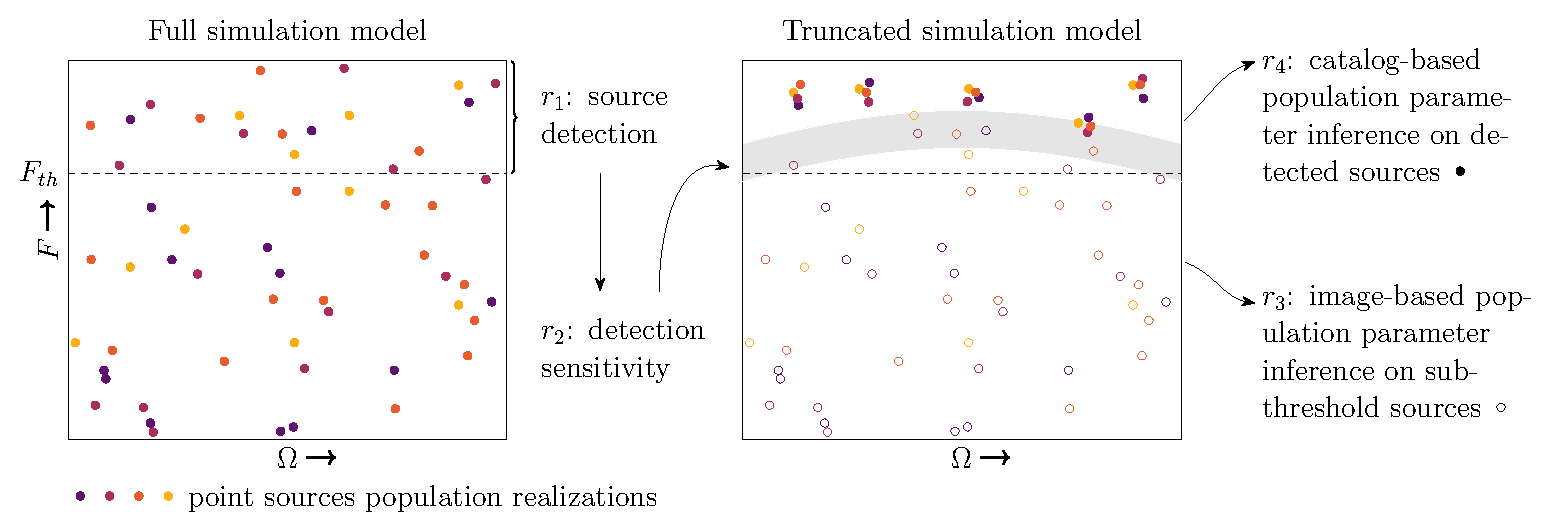
\includegraphics[width=\linewidth]{PS-graphic.pdf}
    \caption{Illustration of our inference framework (see Section~\ref{sec:ps-method} for details). \textit{Left panel}: A source detection network $r_1$ and the corresponding sensitivity network $r_2$ are trained based on the full simulation model. \textit{Right panel}: Bright sources are constrained in the truncated simulation model, while sub-threshold sources vary freely.  Two inference networks are trained to capture information from sub-threshold sources ($r_3$) and detected sources ($r_4$).
    }
    \label{fig:ps-graphic}
\end{figure}


\section{Experiment}
\label{sec:ps-results}

\begin{figure}
    \centering
    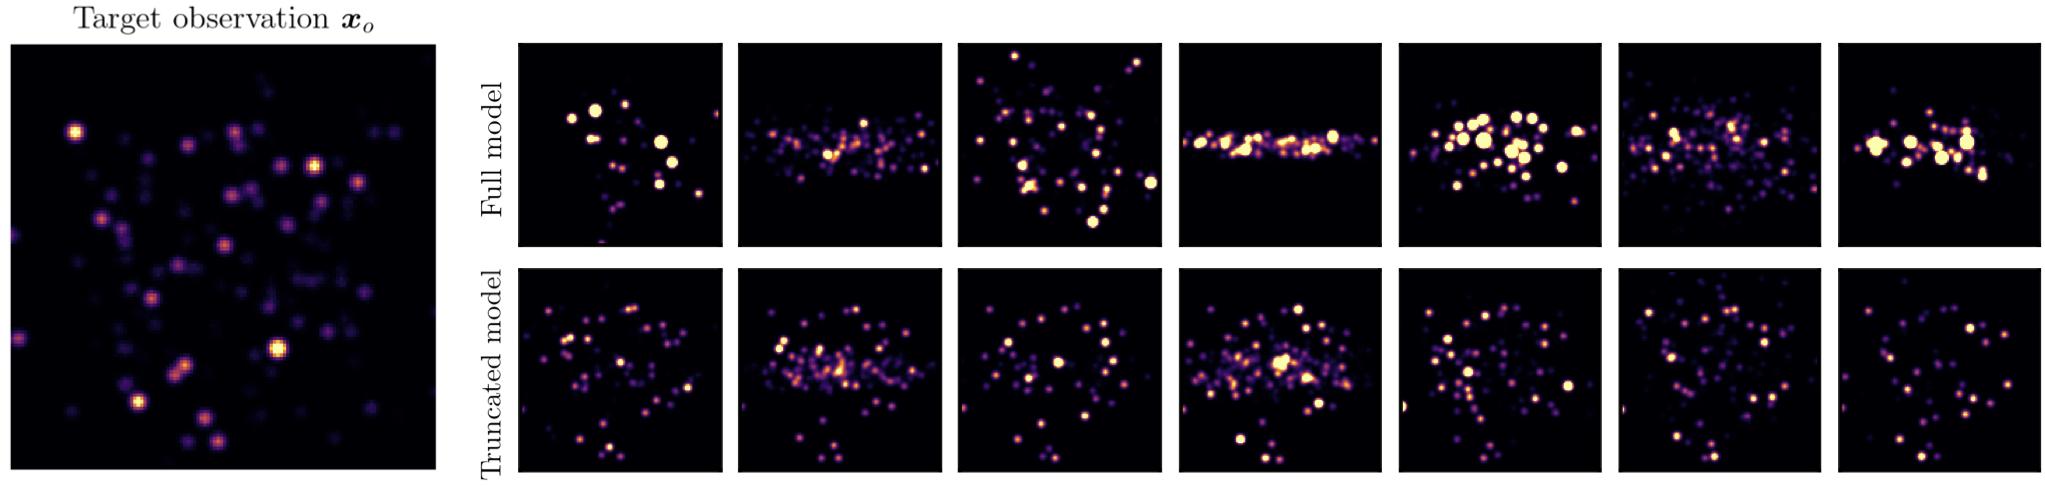
\includegraphics[width=\linewidth, clip=true, trim = 0mm 0mm 16cm 0mm]{PS-data.jpg}
    \caption{
      \textit{Left:} Observation of reference $\data_o$. 
      \textit{Right:} In the first row we show samples from our full simulation model. In the second row we show targeted samples from the truncated model. Targeted data are visually more close to $\data_o$, the main dissimilarities are due to different sub-threshold sources and instrumental effects realizations.
    }
    \label{fig:ps-data}
\end{figure}

\begin{figure}
    \centering
    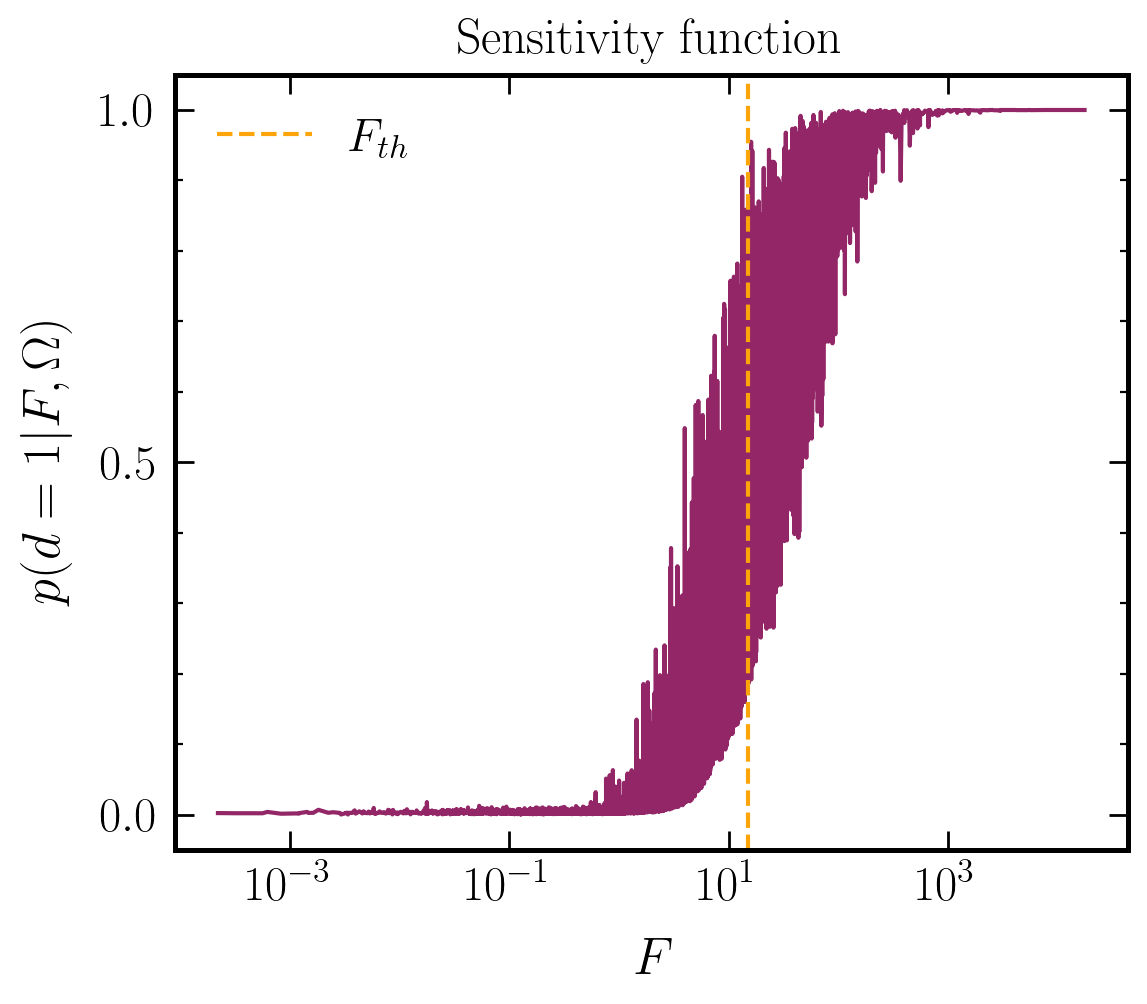
\includegraphics[width=0.6\linewidth]{PS-sensitivity.png}
    \caption{Point source sensitivity function $S(F, \Omega)$ as a function of flux $F$. The function characterizes the split between detected and sub-threshold sources by the source detection network $r_1$, providing the probability that a source with flux $F$ and at position $\Omega$ would be detected by the ratio estimator in Equation~\eqref{eq:ps-rFth}.  
    }
    \label{fig:ps-sensitivity}
\end{figure}

\begin{figure}
\centering
      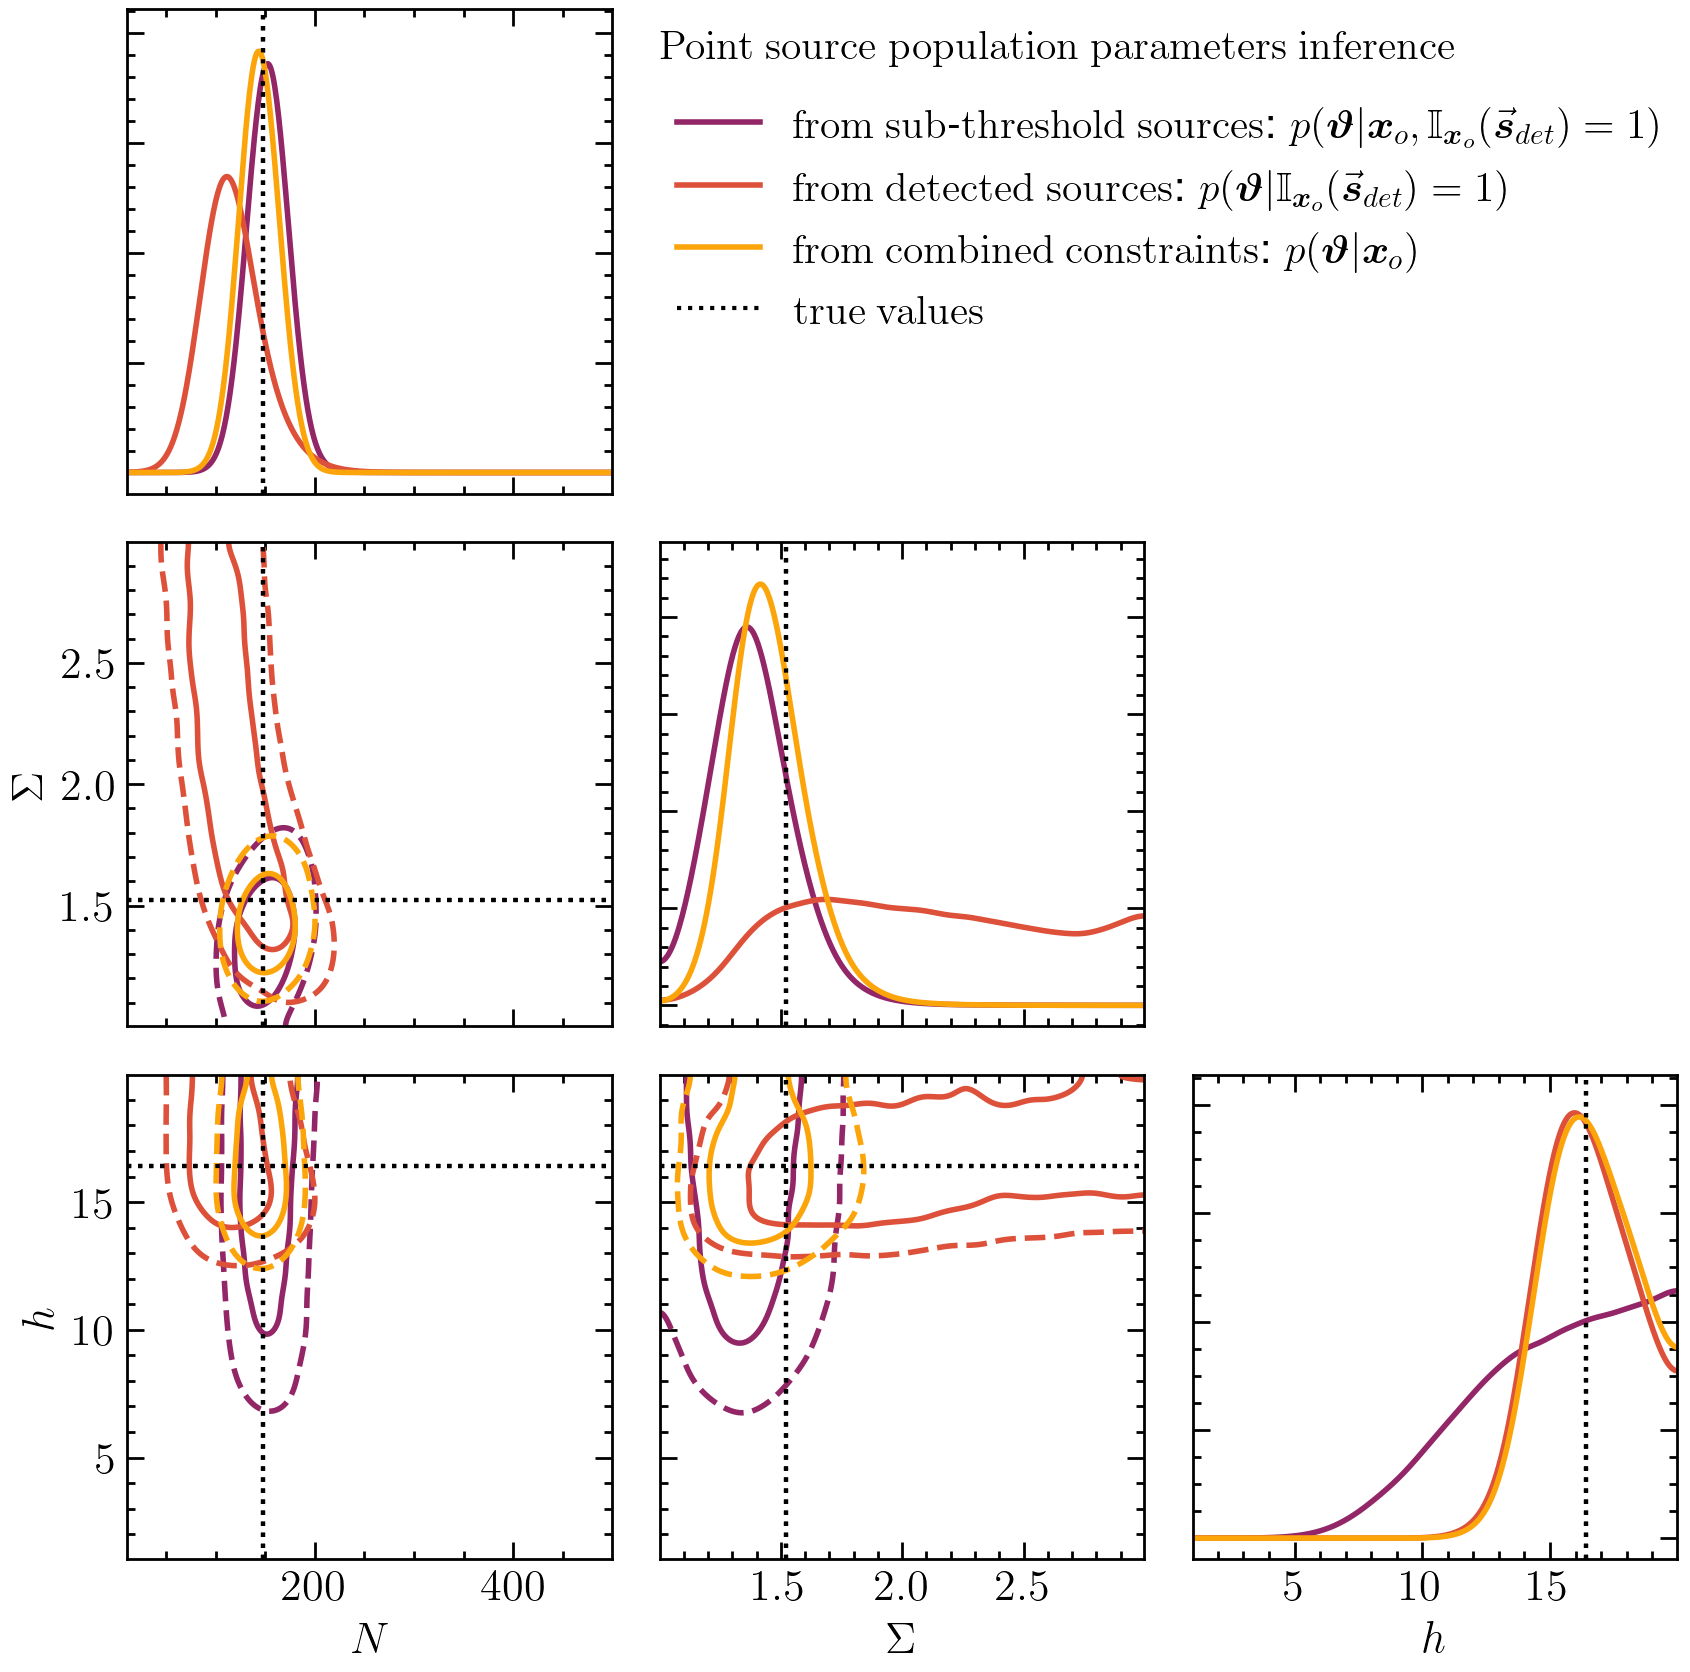
\includegraphics[width=0.75\linewidth]{PS-results.jpg}
    \caption{Marginal posteriors inferred by \gls*{tmnre} on target observation $\data_o$ for population parameters $\interest$. We show constraints from sub-threshold sources (violet), detected sources (orange), and combined results (yellow). In the 2D marginal posterior we indicate the $68\%$ and $95\%$ credible regions with solid and dashed lines respectively. For more details see Section~\ref{sec:ps-results}.
}
\label{fig:ps-results}
\end{figure}

We apply the proposed methodology to the simulated target observation $\data_o$ shown in Figure~\ref{fig:ps-data}. 

\paragraph{Training strategy.} We first train the source detection ratio estimator in Equation~\eqref{eq:ps-rFth} on data simulated from the full model shown in Equation~\eqref{eq:ps-model}, and then apply it to $\data_o$ to obtain a detection map. From the detection map we derive a catalog of detected sources $\vec{\boldsymbol{s}}_{det}$, and define a truncated parameter space of interest, where $\mathbb{I}_{\data_o}(\vec{\boldsymbol{s}}_{det})=1$. In order to make source detection part of our model, we train the sensitivity ratio estimator in Equation~\eqref{eq:ps-rd} to estimate the sensitivity function $S(F, \Omega)$, illustrated in Figure~\ref{fig:ps-sensitivity}. We then generate targeted training data from our truncated simulation model in Equation~\eqref{eq:ps-truncatedmodel}. We show samples from the full model and the truncated one in Figure~\ref{fig:ps-data}. Finally, we train two inference networks to capture information regarding population parameters from sub-threshold and detected sources, as explained in Section~\ref{sec:ps-method}. 
The four neural networks were trained on a NVIDIA GeForce RTX 3080 Ti GPU, the total computational time cost to obtain the results shown in Figure~\ref{fig:ps-results} is $\sim 2$ hours. 

\paragraph{Results.} We show the constraints on population parameters $\interest$  from sub-threshold sources, detected ones, and their combination in Figure~\ref{fig:ps-results}. The different posteriors are consistent with each other, indicating that the proposed inference framework automatically accounts for detection biases. We see that different constraints are dominated by different neural networks, \eg~the number $N$ of point source is better constrained by sub-threshold ones, whereas the spatial distribution parameter $h$ by detected ones. The weaker constraint on the flux parameter $\Sigma$ inferred from detected sources is due to the fact that in Equation~\eqref{eq:ps-average} we average over different detected sources realisations, always re-sampling the parameter $\Sigma$ (see Section~\ref{subsec:ps-sim} for the hierarchical model details).


\section{Discussion and conclusions}
\label{sec:ps-conclusions}

We have introduced a novel method to self-consistently perform point sources detection and source population parameters inference using \gls*{tmnre}. The key realization underlying this methodology is that point source detection is equivalent to prior truncation and essential to reduce training data variance. With this approach, we can exploit information of detected as well as sub-threshold sources for population-level parameter inference. Detection biases are automatically accounted for in our approach. Exemplary results of our approach are presented in Figure~\ref{fig:ps-results}, where we show inference results on source population parameters from both detected point sources and sub-threshold sources separately, as well as their combination. 

Since the proposed method is essentially a specific implementation of  \gls*{tmnre}, we expect that it inherits its positive properties in terms of simulation-efficiency and scalability \cite{Miller:2021aa}. A possible shortcoming of this approach is that multiple neural networks need to be trained self-consistently, which on the other hand have a clear interpretation in terms of traditional analysis pipeline components. A potential application beyond those directly intended is to detectable and sub-threshold substructures in strong gravitational lenses.


%  \paragraph{Broader Impact}
%  \label{par:impact}
%  This work is focusing on the analysis of astronomical surveys that contain point sources population via TMNRE. Variants of the presented approach could find application in other areas of the physical sciences. We do not expect any negative societal impact of the presented methods. However, we recommend the usual caution in inferring scientific conclusions based on a complex methodology.

  
%  \section*{Acknowledgments and Disclosure of Funding}
%  
%  This work is part of a project that has received funding from the European Research Council (ERC) under the European Union’s Horizon 2020 research and innovation program (Grant agreement No. 864035 -- Undark).
%  
%  We acknowledge the use of the \texttt{python} \citep{python} modules, \texttt{matplotlib} \citep{Hunter:2007ouj}, \texttt{numpy} \citep{Harris:2020xlr},  \texttt{scipy} \citep{Virtanen:2019joe}, \texttt{PyTorch} \citep{pytorch}, \texttt{tqdm} \citep{tqdm}, and \texttt{jupyter} \citep{jupyter}.

  

\chapter{Conclusions and Outlook} \label{cha:conclusions}

The primary goal of this thesis is to enable new physics searches by addressing the statistical and computational challenges that arise in the fields of astrophysics and cosmology. 
The analysis of complex data described by intricate models is challenging due to computational limitations. Traditional methods in modern astrophysical and cosmological data analysis are sampling-based inference techniques like Markov-chain Monte Carlo and nested sampling methods. However, these approaches frequently rely on approximate likelihoods and suffer from a significant drawback: the time required to achieve convergence scales poorly with the dimensionality of the explored parameter space. This thesis contributes to develop and establish an alternative approach based on novel \gls*{sbi} techniques, that have seen a remarkable development in recent years. 
%These techniques offer a qualitative shift in our approach to statistical inference and a promising avenue to fully exploit the data potential. 

\subsection*{Summary}

We began in Chapter~\ref{cha:sbi} by describing how \gls*{sbi} approaches achieve robust Bayesian inference given an implicit representation of the likelihood through a generative model. Thanks to their unique properties, one can coherently segment the analysis into manageable tasks (\eg~parameter inference, object detection, image reconstruction) that target distinct lower-dimensional parts, or “blocks”, of a large model. The inference carried out on each block will take into account the uncertainties coming from the other blocks, thus correctly propagating uncertainties between model components. This approach flexibly modularizes the analysis of large models and then coherently synthesizes it for a comprehensive understanding. It enables one to draw conclusions based on the full model, ultimately making the analysis statistically sound, simulation efficient, and versatile. 

Initially, we focused on the analysis of strong lensing images as a dark matter probe (Chapter~\ref{cha:lensing}). This is a primary example of applicability of \gls*{sbi} to a large forward model. Our results demonstrated that a sequential \gls*{sbi} technique called \gls*{tmnre} enables precise marginal and targeted inference, overcoming traditional computational challenges. We further showed the application of hierarchical inference to extract the dark matter cutoff mass signal from a dataset of lenses.

We then tackled the inverse problem that goes from non-linear, non-local mappings of late-time density fields to Gaussian cosmological initial conditions. To this end, we employed autoregressive Gaussian likelihood estimation to model the conditional dependencies between pixels in the density field. Posterior sampling is achieved through a Gibbs sampling algorithm based on exact data augmentation, ensuring efficient exploration of high-dimensional parameter spaces. The proposed approach combines computational efficiency with applicability to generic, non-differentiable forward simulators, making it suitable for broader astrophysical and cosmological data analysis tasks.

Finally, we turned towards the problem of point source detection and population parameter inference in sky-maps. In Chapter~\ref{cha:detection}, we developed a highly interpretable (since it resembles components of traditional survey analysis workflows) \gls*{sbi} framework that allows, for the first time to the authors' knowledge, to perform consistently point source detection and population parameters inference, from both detected and sub-threshold. This was possible by defining source detection as a novel and high-dimensional form of prior truncation to incorporate detected sources into the simulation model.

Overall, this thesis aimed to highlight the potential of \gls*{sbi} for astrophysical data analysis, positioning this framework as an essential part of the modern physics data analysis toolkit.


\subsection*{Outlook}

We are already witnessing a widespread adoption and advancement of simulation-based inference techniques for cosmological and astrophysical data analysis. However, these techniques have yet to realize their full potential, and numerous challenges remain open. Key questions include: Can the selection of optimal neural networks architectures be automatized? How to handle situations with high volume data? What is the most efficient way to sample from constrained likelihood regions in very high dimensions for sequential inference? How to reliably perform goodness-of-fit tests and identify model misspecification? Crucially, the further development of these techniques must be accompanied by the development of robust performance tests and diagnostics. All these open threads, and possibly more, are active areas of research within the community.

Our pursuit to develop powerful, fast, and robust analysis techniques is especially urgent because of the ever-increasing influx and quality of data from current and forthcoming observatories.
The potential for using these observations to uncover new physics in the dark sector are therefore very bright. Now is absolutely an opportune time to explore innovative ways of maximizing the discovery potentials of these datasets. While the approaches presented in this thesis are far from the only interesting avenues for analyzing this wealth of data for new physics searches, they represent concrete steps towards fully exploiting these measurements to refine our understanding of physical laws.
%to search for physics beyond the Standard Model and novel astrophysical phenomena in the scientific feedback-loop.

\todo{Not sure about including this or stop at the paragraph above:}
Indeed, \gls*{sbi} provides approximate solutions for the comparison of complex models with high-quality data, making it a powerful tool when exact methods fall short. While exact methods might offer precise results, they often do so at the cost of oversimplifying the model, which is particularly risky when dealing with detailed data. By embracing the approximate nature of \gls*{sbi}, we can tackle the right questions with the complexity they deserve, yielding more meaningful insights with accurately quantified uncertainty.

%“[...] as emphasized in Rubin (1984), one of the great scientific advantages of simulation analysis of Bayesian methods is the freedom it gives the researcher to formulate appropriate models rather than be overly interested in analytically neat but scientifically inappropriate models.” (Gelman, 1996)
%
%“Far better an approximate answer to the right question, which is often vague, than an exact answer to the wrong question, which can always be made precise. ” (John Tuckey, 1962)






% ======== Backmatter ========
\backmatter
\selectlanguage{english}
\summary{Summary / Samenvatting}{
%In this chapter, we introduced a novel approach using \gls*{tmnre} to analyze strong gravitational lensing systems for dark matter science. Beginning with an overview of strong lensing and its potential to probe dark matter substructures, we developed a pipeline integrating \gls*{tmnre} to infer the cutoff mass in the dark matter halo mass function directly from simulated observations. We discussed the modeling complexities involved, including lens and source parameter uncertainties, substructure effects, and the validation of our methodology. Our results demonstrated that \gls*{tmnre} enables precise marginal and targeted inference, overcoming traditional computational challenges. We further showed the application of hierarchical inference to extract the dark matter cutoff mass signal from a population of substructures, paving the way for future advancements in dark matter characterization using strong lensing observations.
%

\newpage




\textit{Vertaald door Dion Noordhuis.}
}
\acknowledgements{Acknowledgements}{% Acknowledgements ============================================================

\todo{
	\begin{itemize}
		\item Christoph
		\item GRAPPA: Shin'ichiro, Gianfranco, Samaya, Philipp, Jacco, Ben
		\item Secretariat: Jirina...
		\item Gimmy 
		\item Dion, Uddipta, Fabian, Mathis
		\item Oleg, Youyou, Alex, Huyfang, Kate 
		\item Ariane and Banafshe
		\item James
		\item Pippa, Guillermo, Sam, Camila, Malte
		\item Adam and Kosio
		\item Florian
		\item Annecy: Francesca and Christopher
		\item Friends who visited
		\item Fra
		\item Ma e Pa
		\item Gio
	\end{itemize}
}

\vskip 2pt


%I am also very grateful to Rafael Porto, who in many ways took on an informal role as my second advisor. He had been influential in encouraging me to venture into gravitational-wave physics, and I have since learned a lot from him about the field. Rafael's excitement about physics is always palpable during our discussions. He would never hesitate to provide me the most candid of advices when I needed them, which is something that I have always appreciated.  
%
%\vskip 2pt
%
%I must thank my wonderful collaborator, John Stout, for his significant contributions to this thesis. Among his many strengths, John's patience, depth of thought, and Mathematica wizardry never cease to amaze me. We discussed physics from day to (mid)night, through which I have learned a lot from him. Though I occasionally regret his irreversible influence on me into compulsive daily-intake of coffee, I am glad to have known him as a great friend.
%
%
%\vskip 2pt
%
%Halfway through my PhD, Samaya Nissanke joined the university as a new faculty member. She has since become the light that brightens up the department through her compassion and openness to scientific research. Samaya's arrival has also attracted a large influx of experts in gravitational-wave physics to the department, many whom I have interacted regularly. Above all, I am grateful for her continuous support and encouragement.
%
%
%\newpage
%
%
%I'd also like to thank Asimina Arvanitaki and Savas Dimopoulos for sharing their insights in particle physics and inspiring me with their scientific creativity. Their insistences on me to provide numbers and do quick checks on the observability of an idea have certainly had an impact on the way I do science. 
%
%\vskip 2pt
%
%To my collaborators: Christoffel Doorman, Thomas Edwards, Tanja Hinderer, and Lotte ter Haar -- thank you all for the enjoyable times we have had doing science together. I have learned a lot from all of you.
%
%
%\vskip 2pt
%
%For stimulating physics discussions, I'd also like to thank Mustafa Amin, Masha Baryakhtar, Gianfranco Bertone, Diego Blas, Beatrice Bonga, Katy Clough, David Cyncynates, Liang Dai, Sam Dolan, Will East, Marcos Garcia, Tudor Giurgic$\check{a}$-Tiron, Daniel Green, Junwu Huang, Badri Krishnan, Robert Lasenby, Eugene Lim, Krista Lynne, David Nichols, Roberto Oliveri, Frans Pretorius, Bob Wagoner, Dan Wilkins, Helvi Witek, Huan Yang, Matias Zaldarriaga, Jun Zhang, and Aaron Zimmerman. 
%
%\vskip 2pt
%
%
%Many other people have made my time in Amsterdam a great pleasure. To the cosmology group members: Matteo Biagetti, Carlos Duaso Pueyo,  Garrett Goon, Austin Joyce, Hayden Lee, Guilherme Pimentel, and  Benjamin Wallisch; thank you all for the great friendships. Group lunches and speakers' dinners will always be memorable times of my PhD. I'd also like to thank my fellow graduate students, to name a few: Gr\'egoire Mathys, Antonio Rotundo, Ka Wa Tsang, and Dong-Gang Wang, for making my graduate experience far more enjoyable.
%
%\vskip 2pt
%
%My graduate experience had been greatly enriched by my extended visits to the Henri Poincar\'e Institute, Perimeter Institute, and the Stanford Institute for Theoretical Physics. I thank these institutes for their kind hospitality and for providing intellectually-stimulating environments. Special thanks to King's College London for always offering me a desk during my visits to London.  
%
%\vskip 2pt
%
%As an engineering freshman eight years ago, I could not had foreseen myself switching to physics, let alone pursuing a doctorate in this field. For this I am grateful to Andrew Jardine and Matthew Wingate for supporting my transitions to the Cavendish Laboratory and DAMTP at Cambridge. %
%
%\vskip 2pt
%
%My family has played a pivotal role in my personal growth and development. A career in academic research is uncommon in our culture, yet they have shown unwavering support in my choices. To my mother, Audrey Chin, thank you for your unconditional love and for being my pillar of support. It is hard to overstate how important you have been to my upbringing. To my siblings, Shin Miin Chia and Shin Li Chia, thank you for all the memorable times we have spent together. 
%
%\newpage
%
%To my fianc\'ee, Zhao Feng Ooi, thank you for your love and emotional support throughout these years. Your infectious cheerfulness and optimism are my eternal source of joy. You have made me a better person. I look forward to our adventure ahead and spending the rest of my life with you.
%
%
%\vskip 2pt
%
%More than anyone else, I am indebted to my late father, Ming Chew Chia, without whom none of the opportunities I have had would be possible. His perseverance against all odds has always been my source of inspiration. I cannot thank him enough for the love and care he had provided to our family.

}

% ======== Bibliography ========
\newpage
\phantomsection
\bibliographystyle{utphys}
\bibliography{thesis}
\end{document}



